\documentclass{article}\usepackage[]{graphicx}\usepackage[]{color}
%% maxwidth is the original width if it is less than linewidth
%% otherwise use linewidth (to make sure the graphics do not exceed the margin)
\makeatletter
\def\maxwidth{ %
  \ifdim\Gin@nat@width>\linewidth
    \linewidth
  \else
    \Gin@nat@width
  \fi
}
\makeatother

\definecolor{fgcolor}{rgb}{0.345, 0.345, 0.345}
\newcommand{\hlnum}[1]{\textcolor[rgb]{0.686,0.059,0.569}{#1}}%
\newcommand{\hlstr}[1]{\textcolor[rgb]{0.192,0.494,0.8}{#1}}%
\newcommand{\hlcom}[1]{\textcolor[rgb]{0.678,0.584,0.686}{\textit{#1}}}%
\newcommand{\hlopt}[1]{\textcolor[rgb]{0,0,0}{#1}}%
\newcommand{\hlstd}[1]{\textcolor[rgb]{0.345,0.345,0.345}{#1}}%
\newcommand{\hlkwa}[1]{\textcolor[rgb]{0.161,0.373,0.58}{\textbf{#1}}}%
\newcommand{\hlkwb}[1]{\textcolor[rgb]{0.69,0.353,0.396}{#1}}%
\newcommand{\hlkwc}[1]{\textcolor[rgb]{0.333,0.667,0.333}{#1}}%
\newcommand{\hlkwd}[1]{\textcolor[rgb]{0.737,0.353,0.396}{\textbf{#1}}}%
\let\hlipl\hlkwb

\usepackage{framed}
\makeatletter
\newenvironment{kframe}{%
 \def\at@end@of@kframe{}%
 \ifinner\ifhmode%
  \def\at@end@of@kframe{\end{minipage}}%
  \begin{minipage}{\columnwidth}%
 \fi\fi%
 \def\FrameCommand##1{\hskip\@totalleftmargin \hskip-\fboxsep
 \colorbox{shadecolor}{##1}\hskip-\fboxsep
     % There is no \\@totalrightmargin, so:
     \hskip-\linewidth \hskip-\@totalleftmargin \hskip\columnwidth}%
 \MakeFramed {\advance\hsize-\width
   \@totalleftmargin\z@ \linewidth\hsize
   \@setminipage}}%
 {\par\unskip\endMakeFramed%
 \at@end@of@kframe}
\makeatother

\definecolor{shadecolor}{rgb}{.97, .97, .97}
\definecolor{messagecolor}{rgb}{0, 0, 0}
\definecolor{warningcolor}{rgb}{1, 0, 1}
\definecolor{errorcolor}{rgb}{1, 0, 0}
\newenvironment{knitrout}{}{} % an empty environment to be redefined in TeX

\usepackage{alltt}
\usepackage{authblk}
\usepackage{float}
\usepackage{multirow}
\usepackage[utf8]{inputenc}
\IfFileExists{upquote.sty}{\usepackage{upquote}}{}
\begin{document}
\title{}
\author{}
\maketitle




\section{Description}



\section{Overview}


\begin{knitrout}
\definecolor{shadecolor}{rgb}{0.969, 0.969, 0.969}\color{fgcolor}
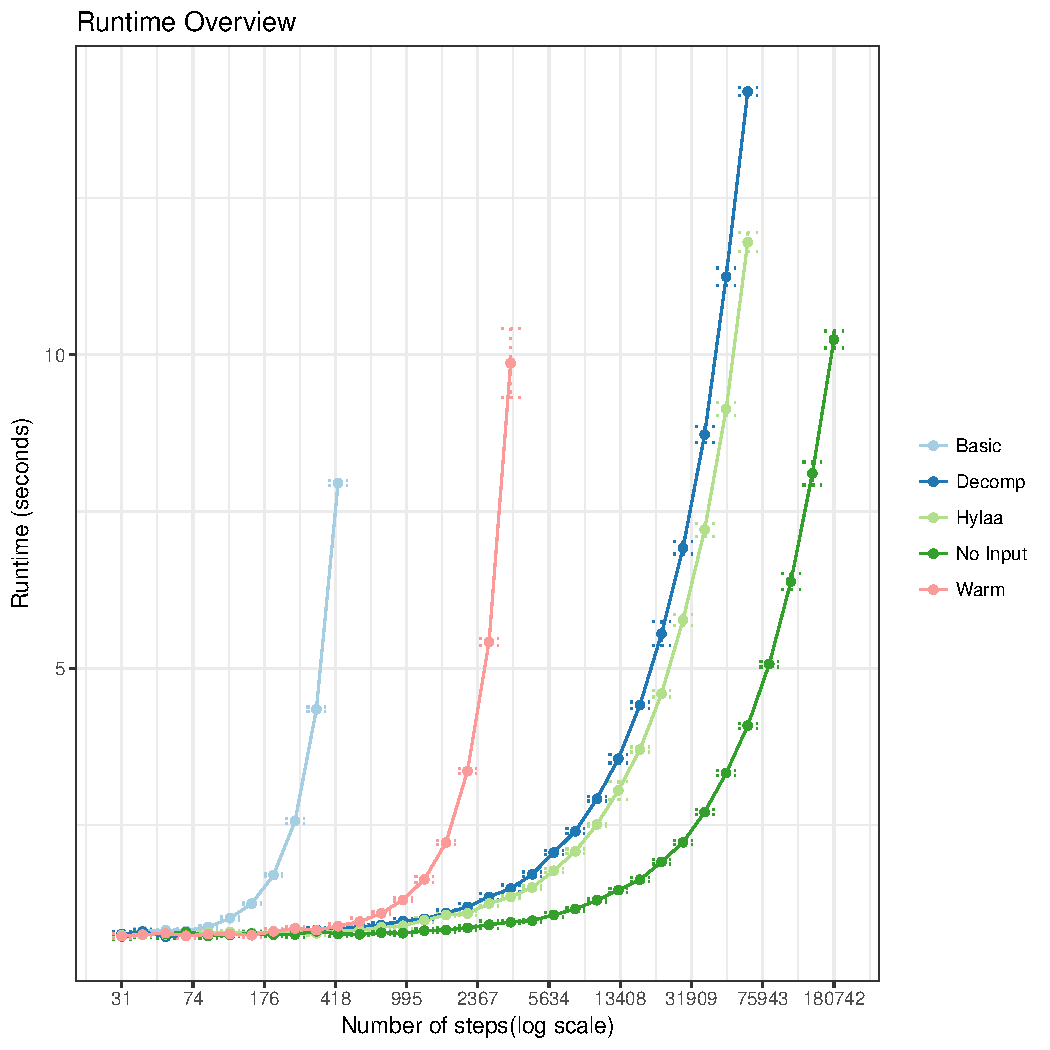
\includegraphics[width=\maxwidth]{figure/overview_time-1} 

\end{knitrout}



\subsection{Objects Overview}
\subsubsection{Overview for 31 steps}
\begin{knitrout}
\definecolor{shadecolor}{rgb}{0.969, 0.969, 0.969}\color{fgcolor}
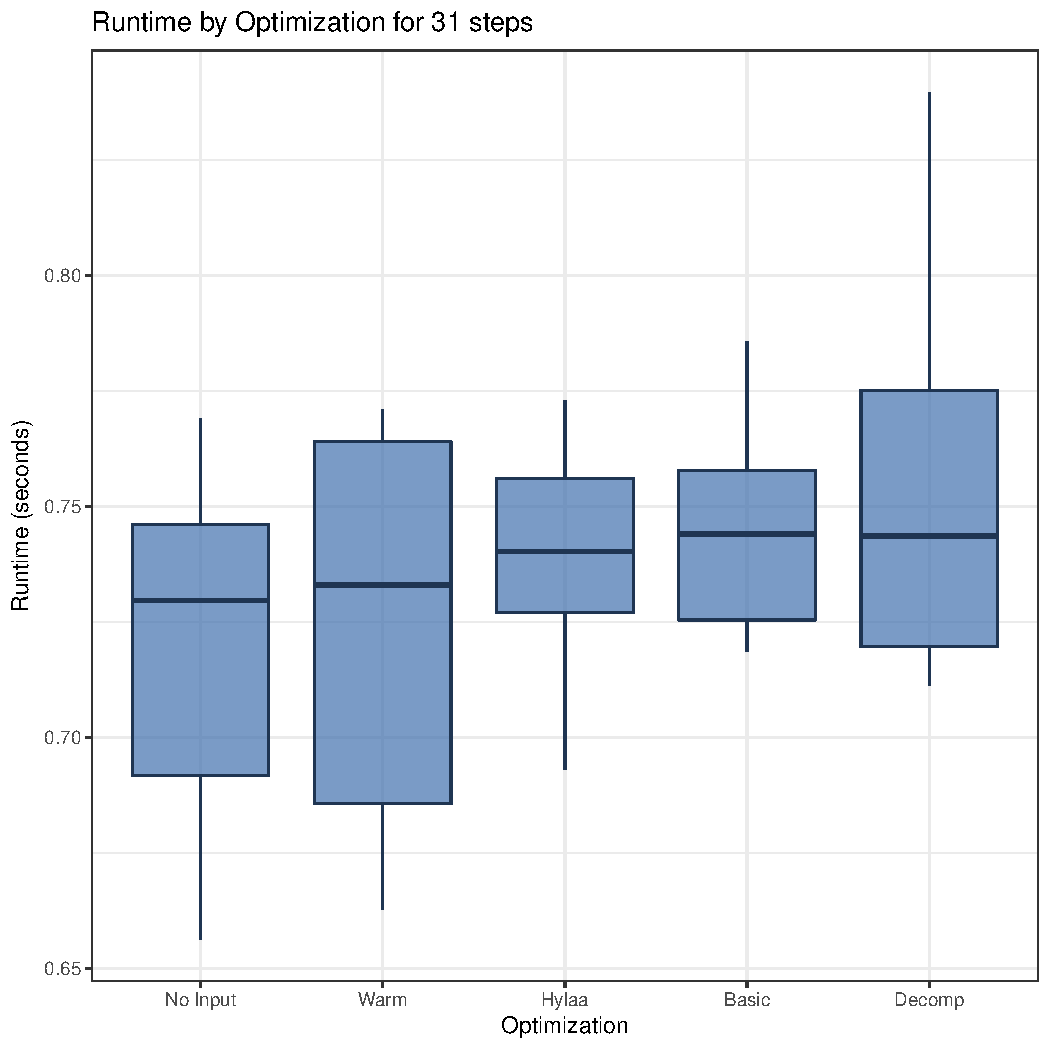
\includegraphics[width=\maxwidth]{figure/steps31-1} 

\end{knitrout}
\subsubsection{Overview for 40 steps}
\begin{knitrout}
\definecolor{shadecolor}{rgb}{0.969, 0.969, 0.969}\color{fgcolor}
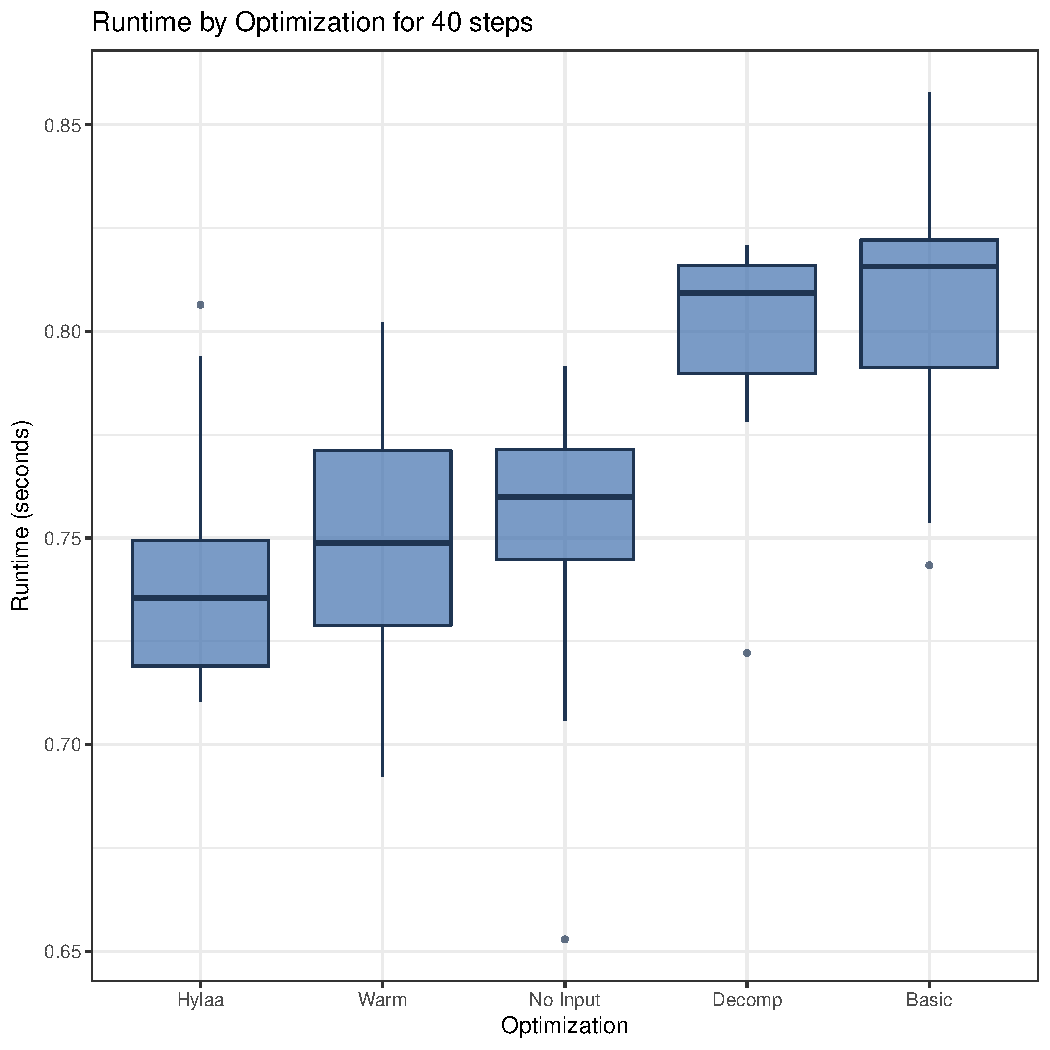
\includegraphics[width=\maxwidth]{figure/steps40-1} 

\end{knitrout}
\subsubsection{Overview for 53 steps}
\begin{knitrout}
\definecolor{shadecolor}{rgb}{0.969, 0.969, 0.969}\color{fgcolor}
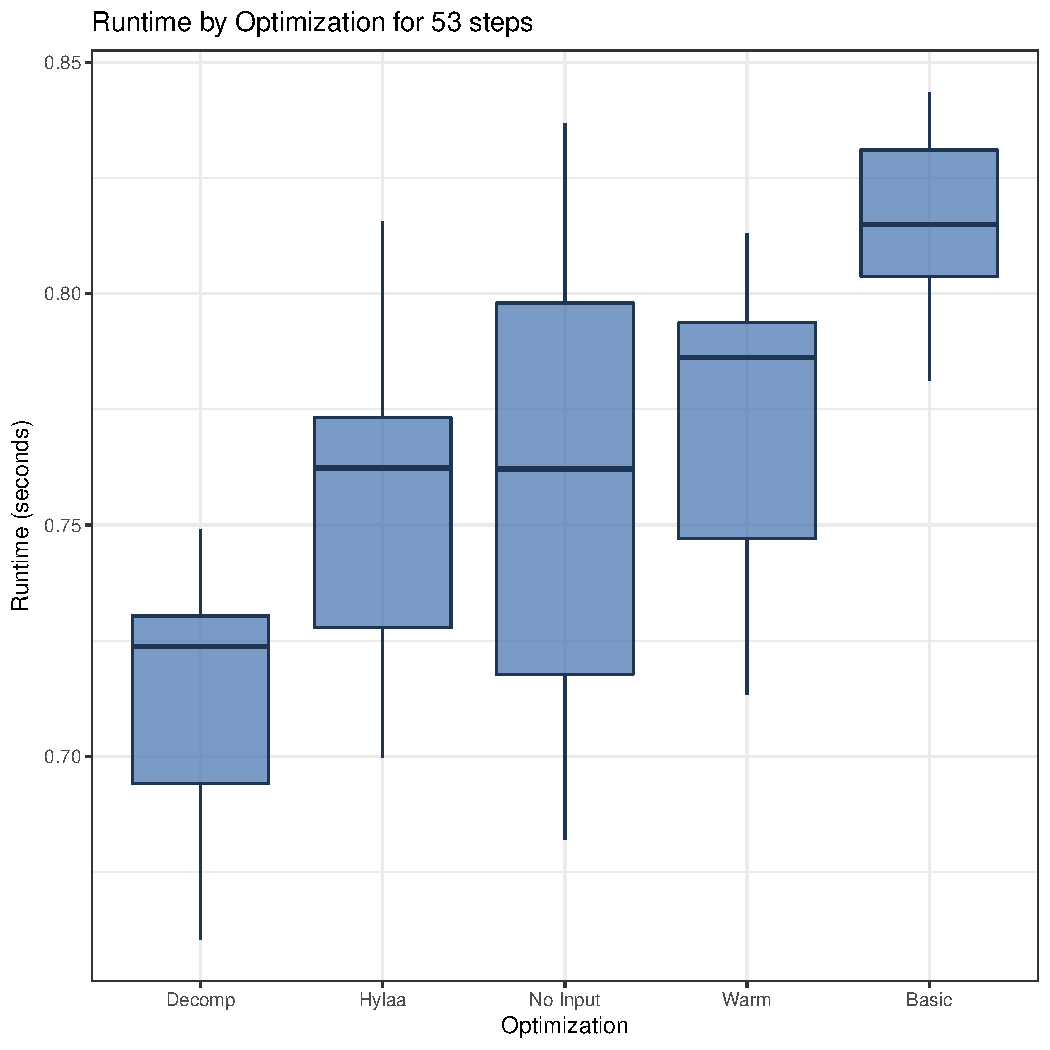
\includegraphics[width=\maxwidth]{figure/steps53-1} 

\end{knitrout}
\subsubsection{Overview for 68 steps}
\begin{knitrout}
\definecolor{shadecolor}{rgb}{0.969, 0.969, 0.969}\color{fgcolor}
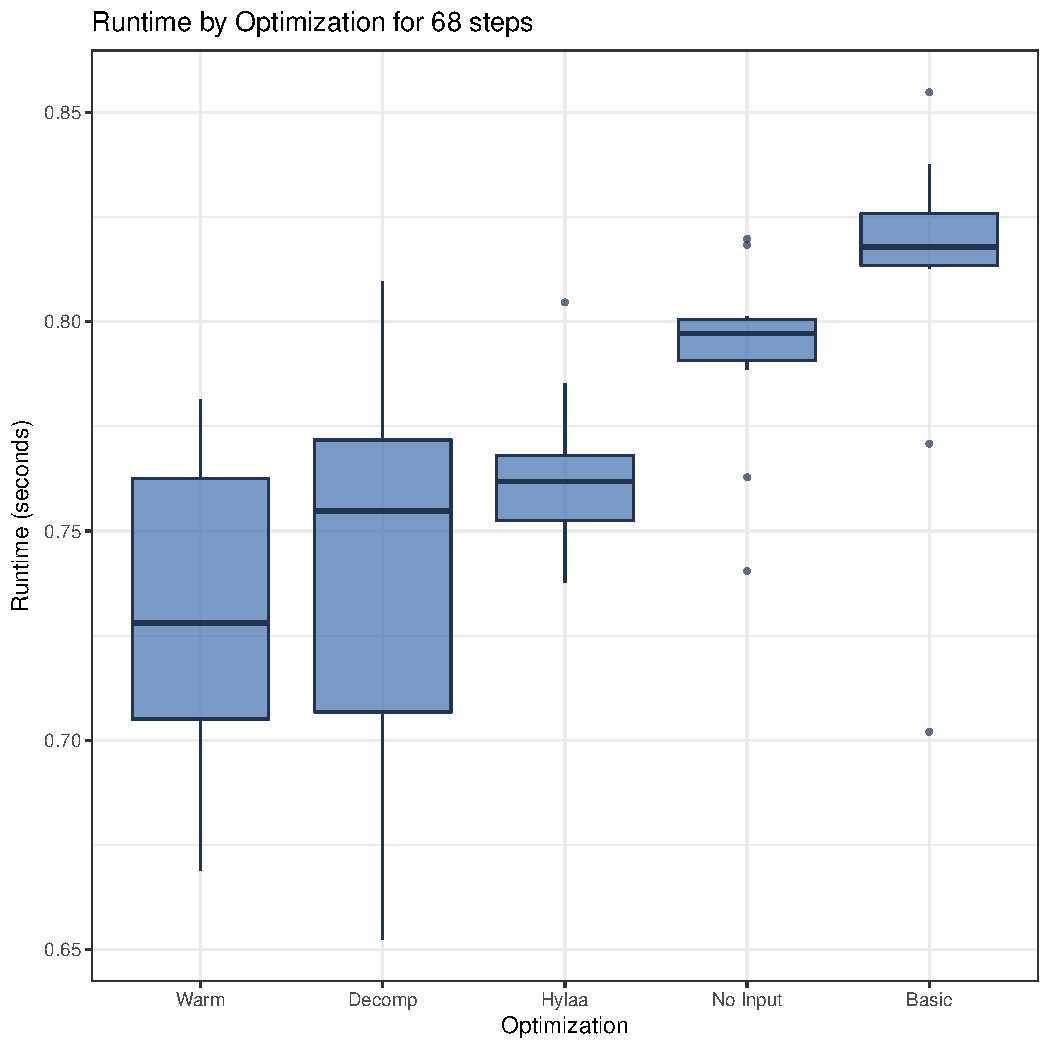
\includegraphics[width=\maxwidth]{figure/steps68-1} 

\end{knitrout}
\subsubsection{Overview for 89 steps}
\begin{knitrout}
\definecolor{shadecolor}{rgb}{0.969, 0.969, 0.969}\color{fgcolor}
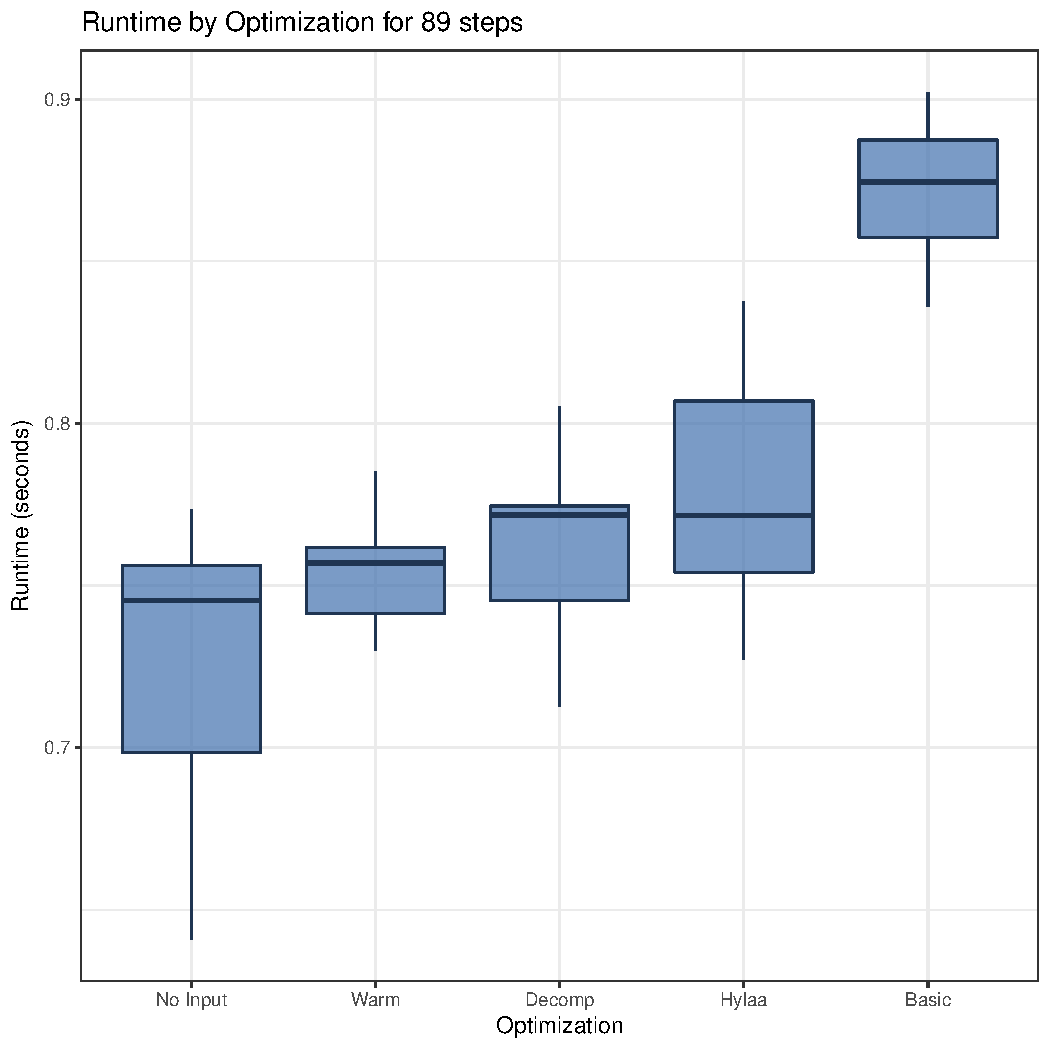
\includegraphics[width=\maxwidth]{figure/steps89-1} 

\end{knitrout}
\subsubsection{Overview for 116 steps}
\begin{knitrout}
\definecolor{shadecolor}{rgb}{0.969, 0.969, 0.969}\color{fgcolor}
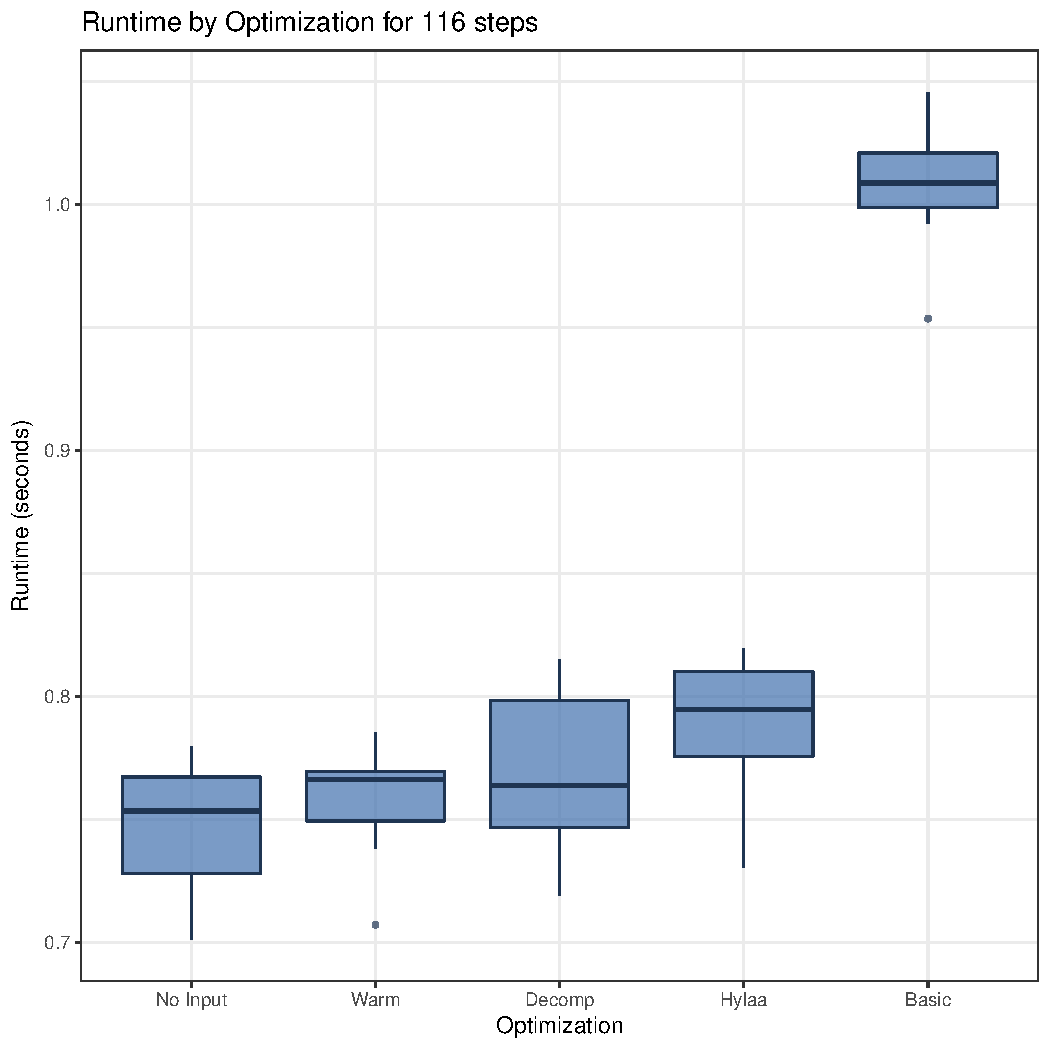
\includegraphics[width=\maxwidth]{figure/steps116-1} 

\end{knitrout}
\subsubsection{Overview for 151 steps}
\begin{knitrout}
\definecolor{shadecolor}{rgb}{0.969, 0.969, 0.969}\color{fgcolor}
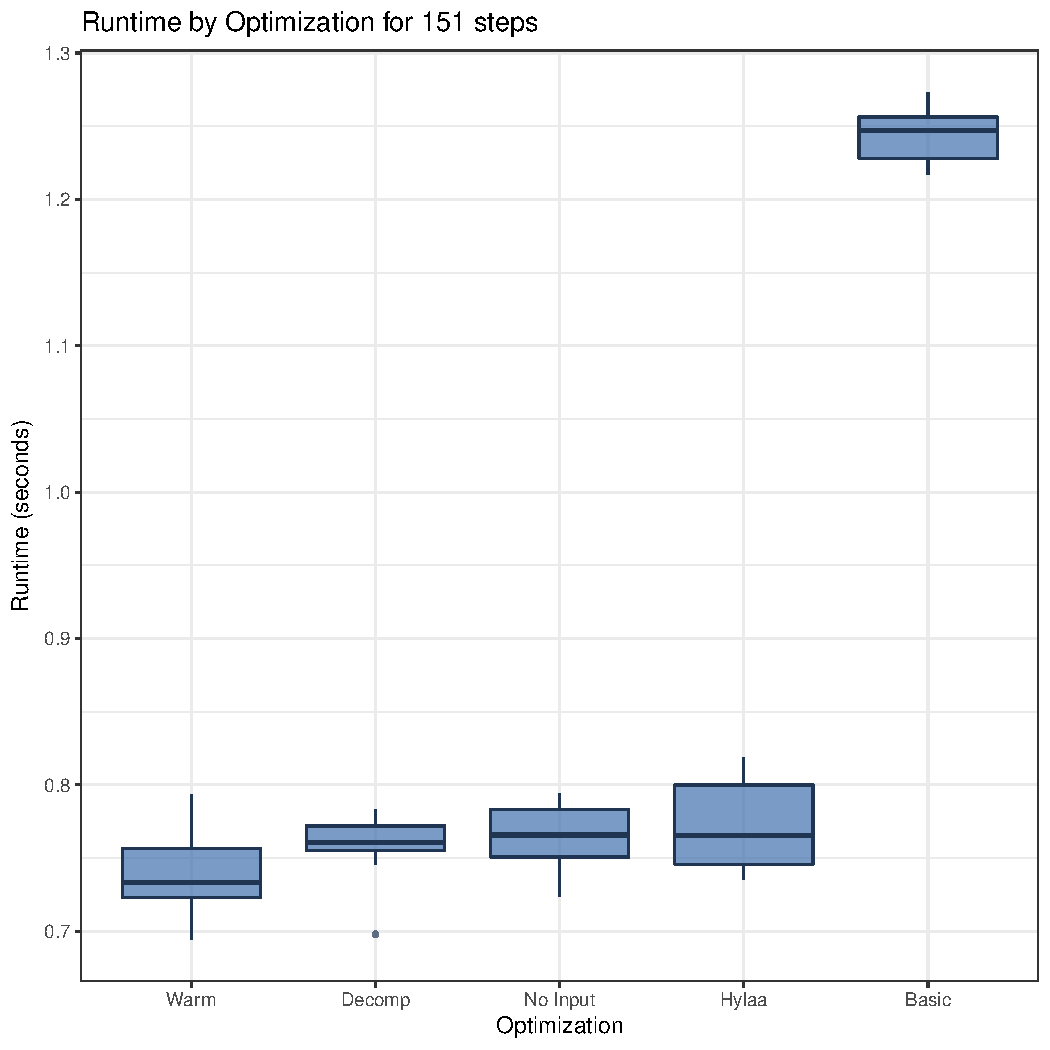
\includegraphics[width=\maxwidth]{figure/steps151-1} 

\end{knitrout}
\subsubsection{Overview for 197 steps}
\begin{knitrout}
\definecolor{shadecolor}{rgb}{0.969, 0.969, 0.969}\color{fgcolor}
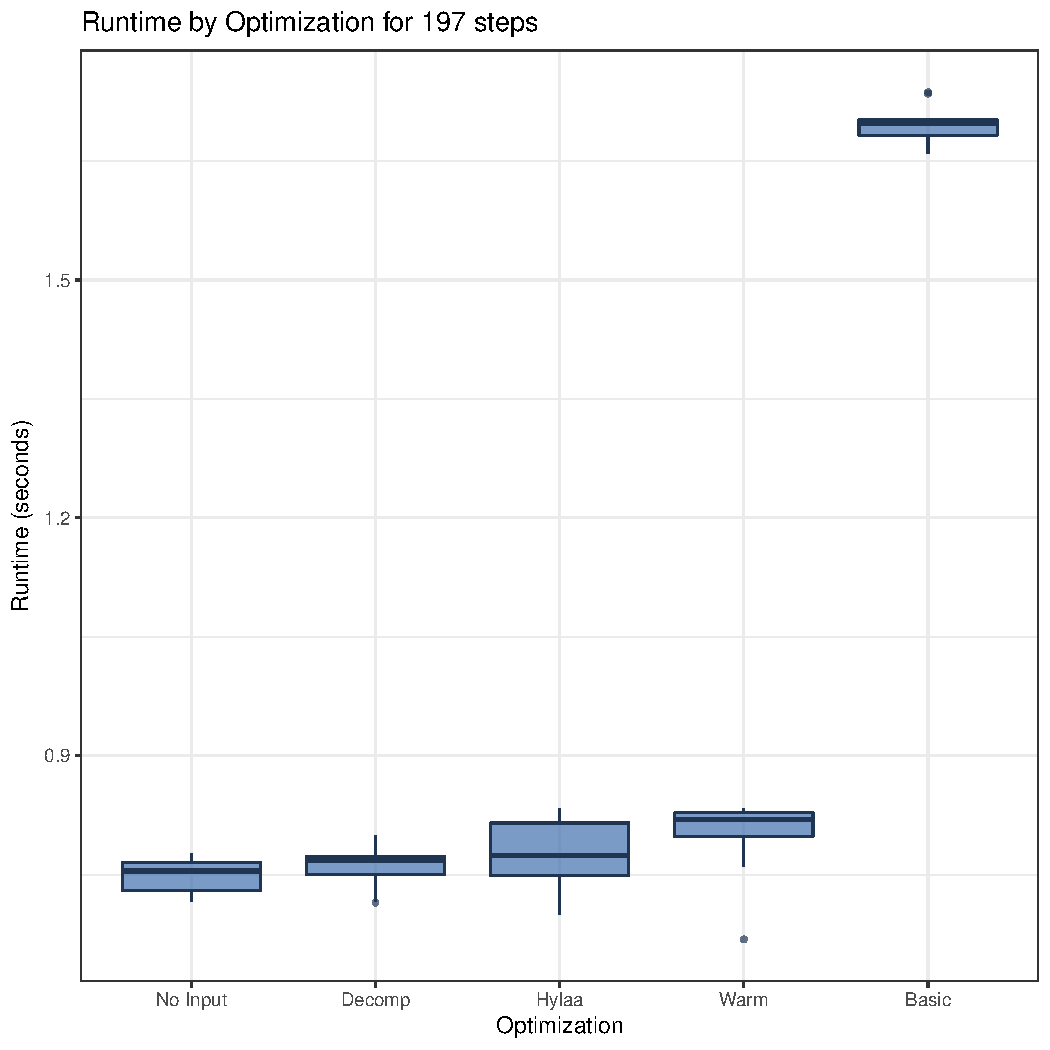
\includegraphics[width=\maxwidth]{figure/steps197-1} 

\end{knitrout}
\subsubsection{Overview for 256 steps}
\begin{knitrout}
\definecolor{shadecolor}{rgb}{0.969, 0.969, 0.969}\color{fgcolor}
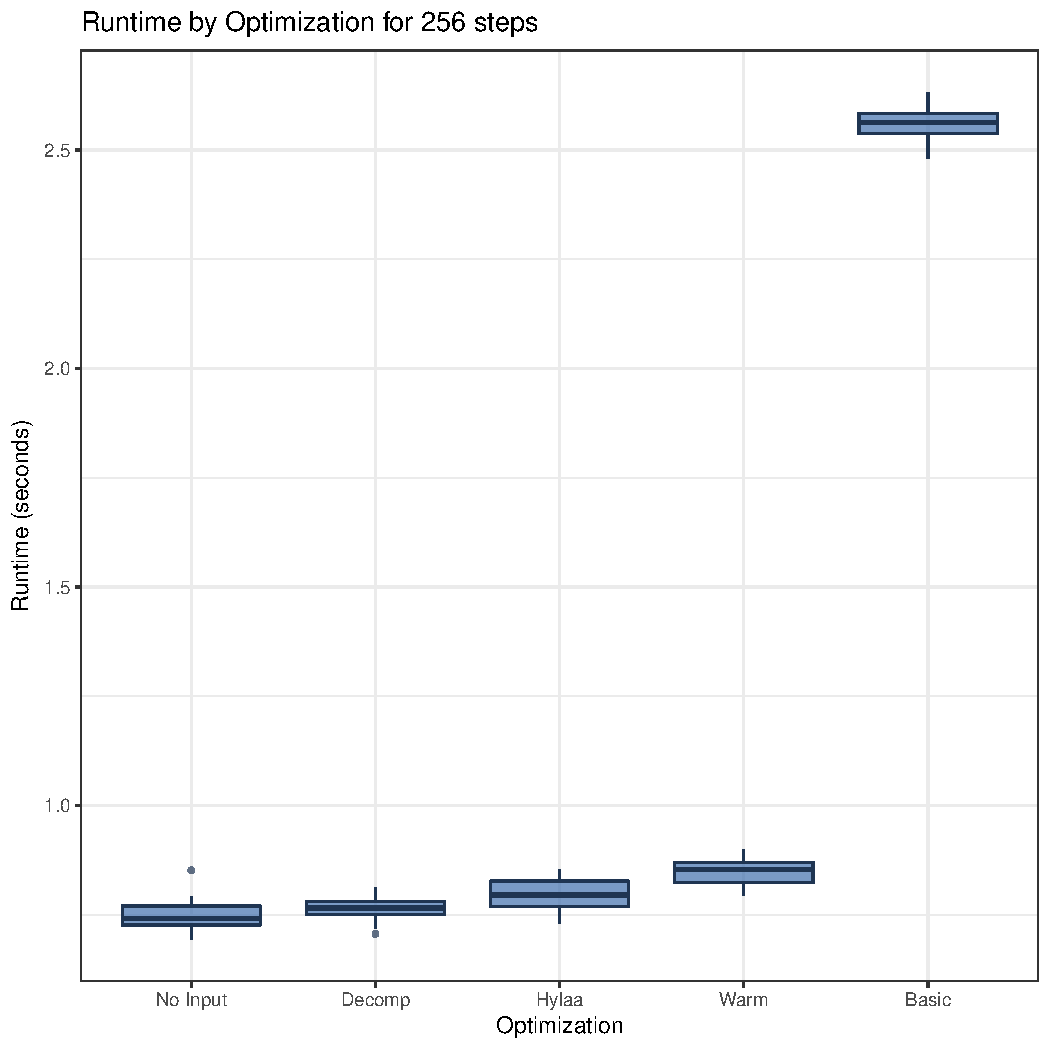
\includegraphics[width=\maxwidth]{figure/steps256-1} 

\end{knitrout}
\subsubsection{Overview for 332 steps}
\begin{knitrout}
\definecolor{shadecolor}{rgb}{0.969, 0.969, 0.969}\color{fgcolor}
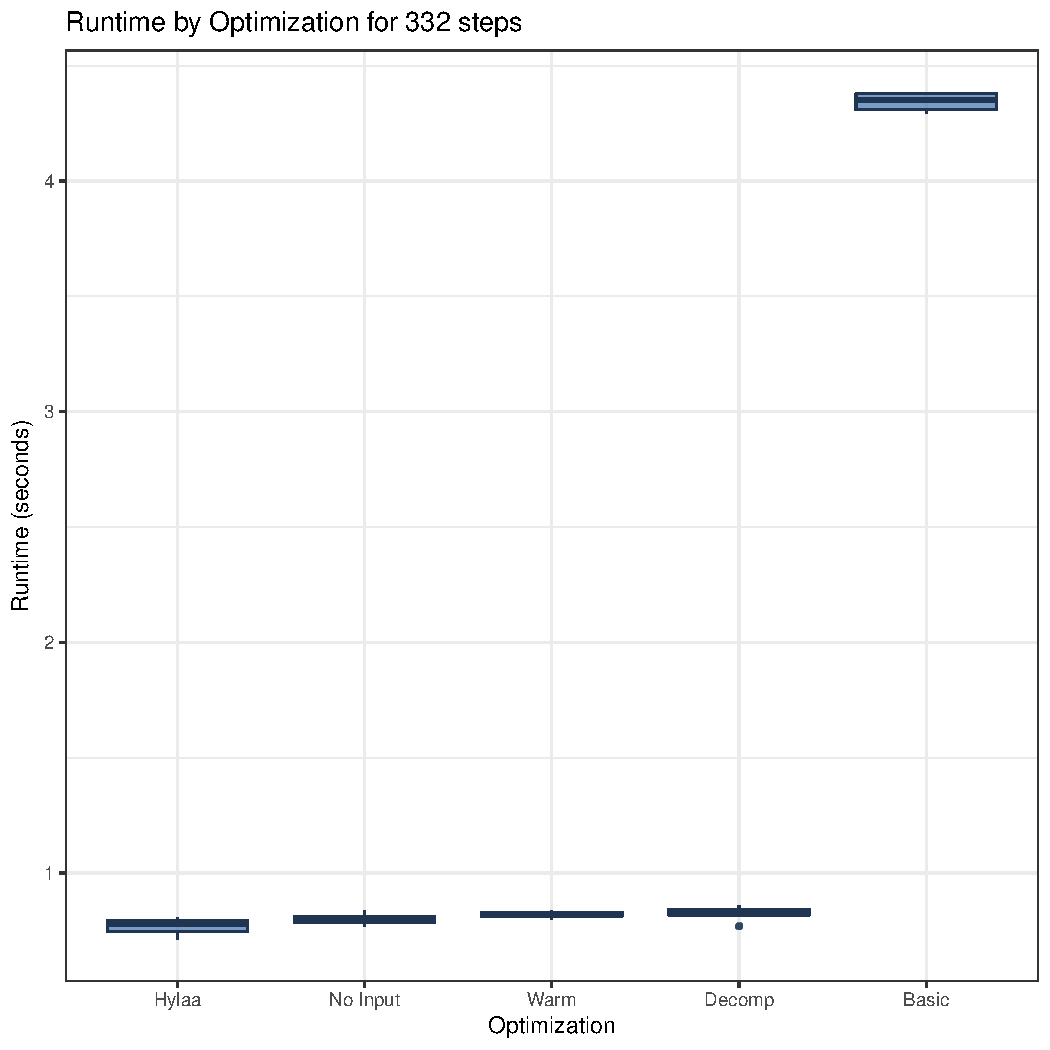
\includegraphics[width=\maxwidth]{figure/steps332-1} 

\end{knitrout}
\subsubsection{Overview for 432 steps}
\begin{knitrout}
\definecolor{shadecolor}{rgb}{0.969, 0.969, 0.969}\color{fgcolor}
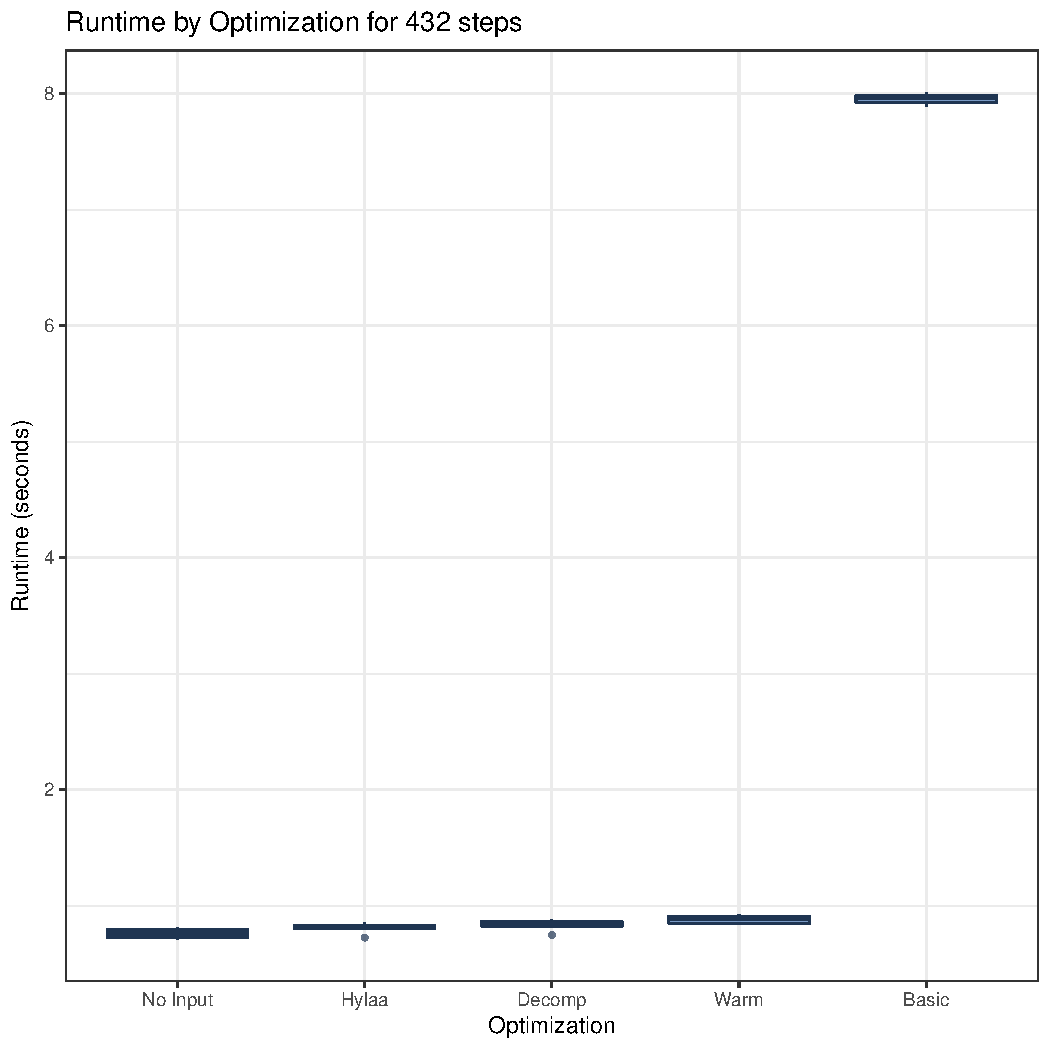
\includegraphics[width=\maxwidth]{figure/steps432-1} 

\end{knitrout}
\subsubsection{Overview for 562 steps}
\begin{knitrout}
\definecolor{shadecolor}{rgb}{0.969, 0.969, 0.969}\color{fgcolor}
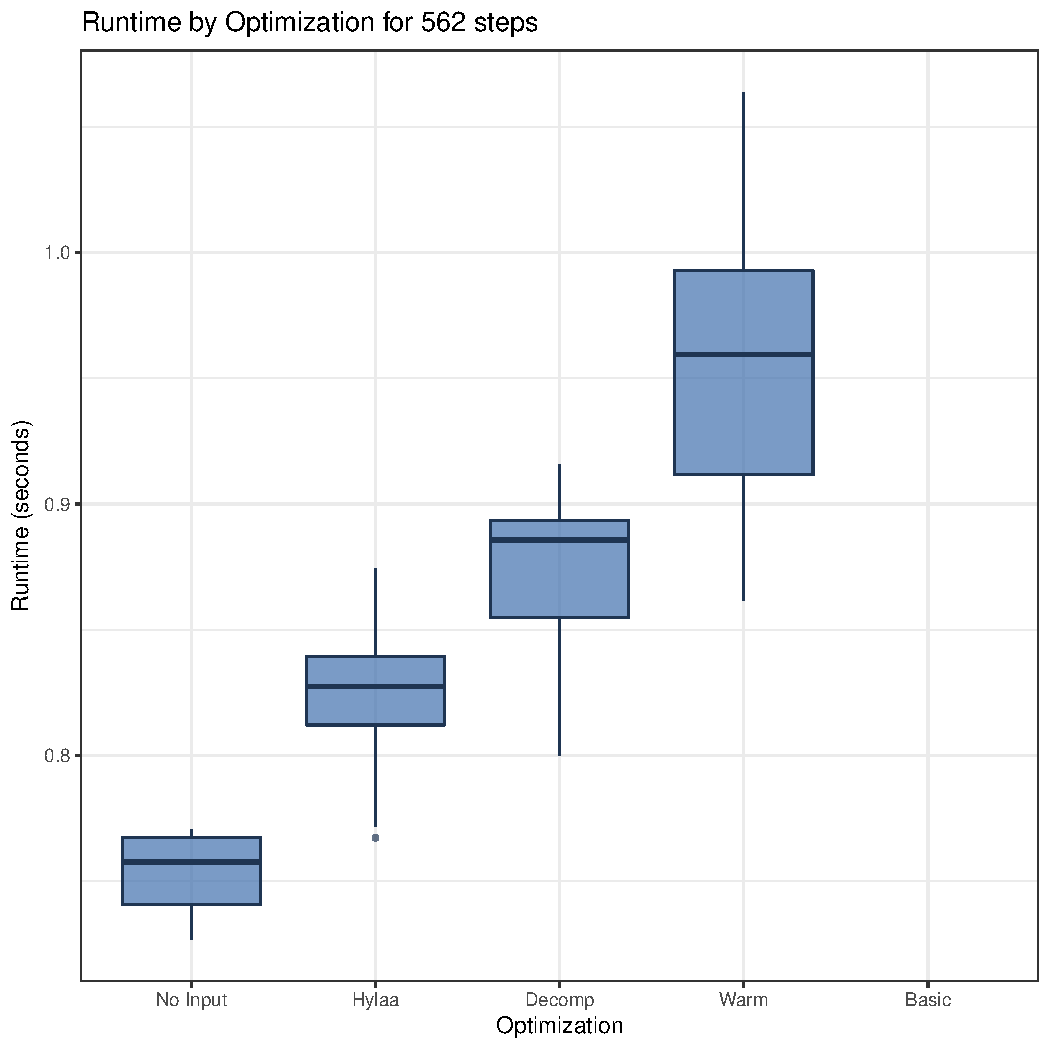
\includegraphics[width=\maxwidth]{figure/steps562-1} 

\end{knitrout}
\subsubsection{Overview for 731 steps}
\begin{knitrout}
\definecolor{shadecolor}{rgb}{0.969, 0.969, 0.969}\color{fgcolor}
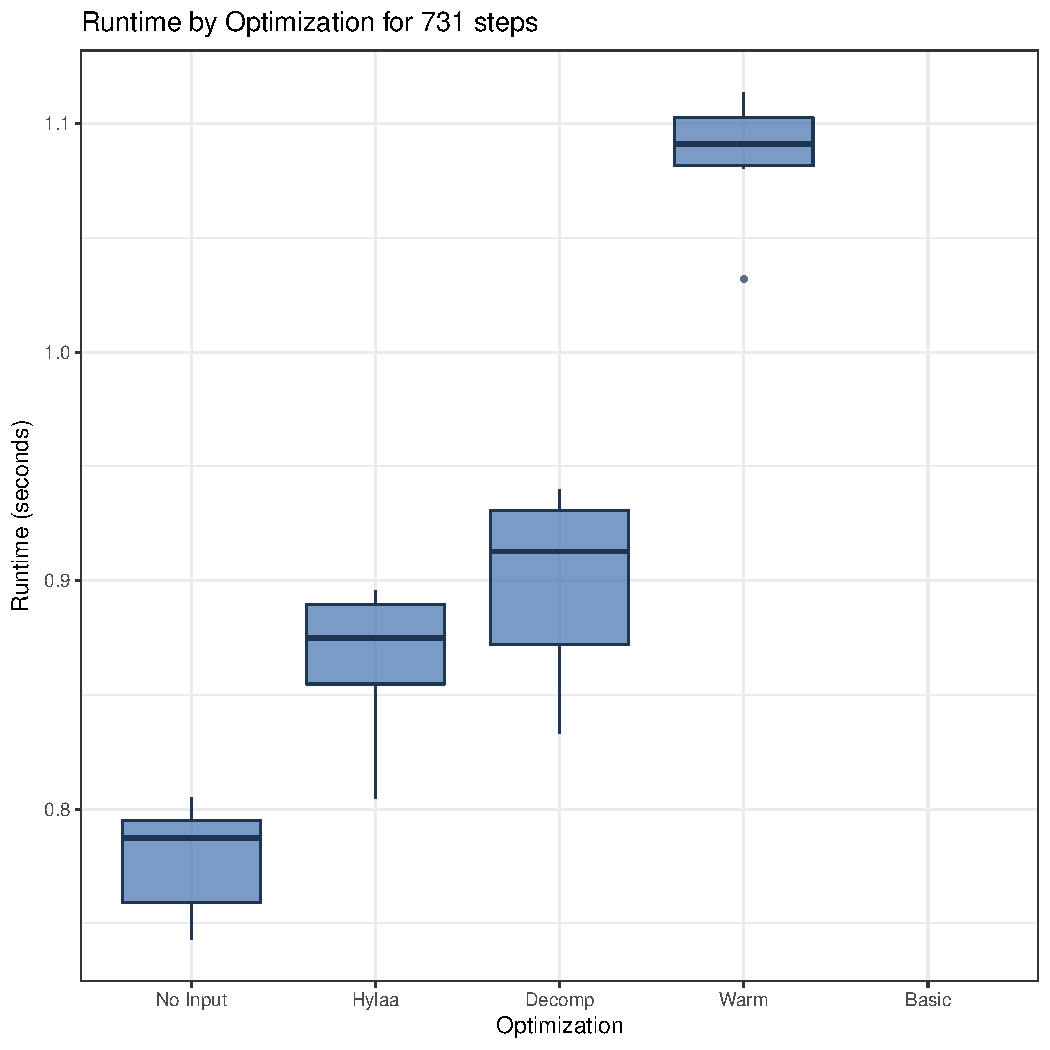
\includegraphics[width=\maxwidth]{figure/steps731-1} 

\end{knitrout}
\subsubsection{Overview for 951 steps}
\begin{knitrout}
\definecolor{shadecolor}{rgb}{0.969, 0.969, 0.969}\color{fgcolor}
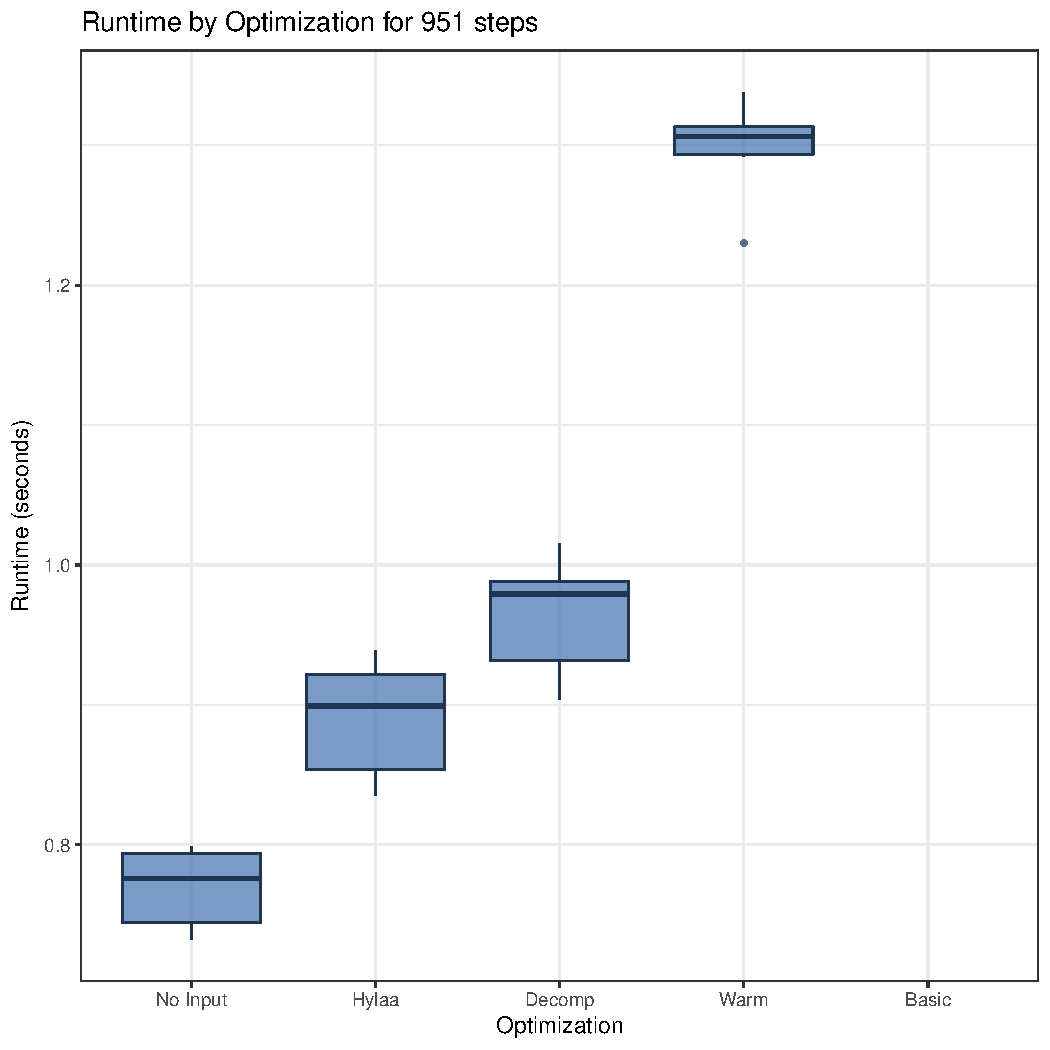
\includegraphics[width=\maxwidth]{figure/steps951-1} 

\end{knitrout}
\subsubsection{Overview for 1236 steps}
\begin{knitrout}
\definecolor{shadecolor}{rgb}{0.969, 0.969, 0.969}\color{fgcolor}
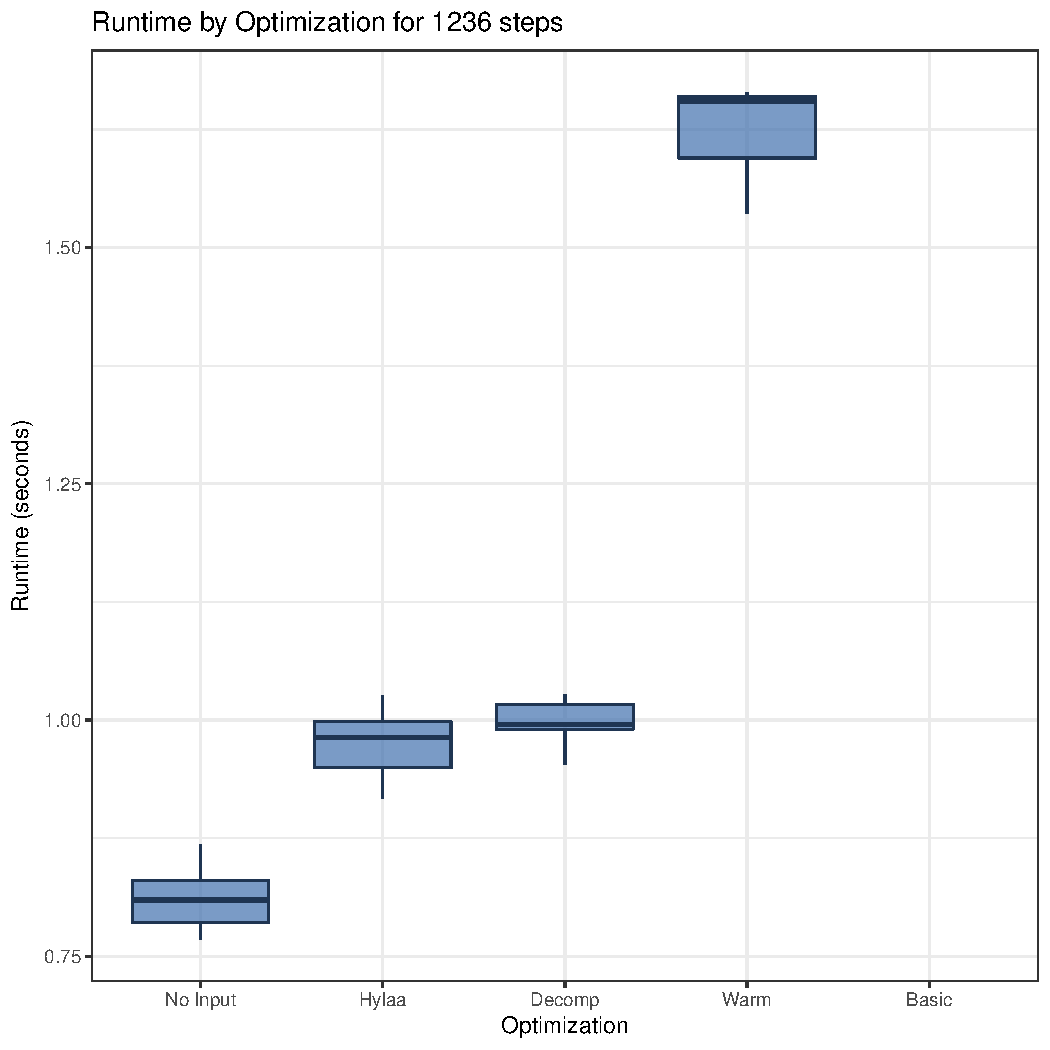
\includegraphics[width=\maxwidth]{figure/steps1236-1} 

\end{knitrout}
\subsubsection{Overview for 1607 steps}
\begin{knitrout}
\definecolor{shadecolor}{rgb}{0.969, 0.969, 0.969}\color{fgcolor}
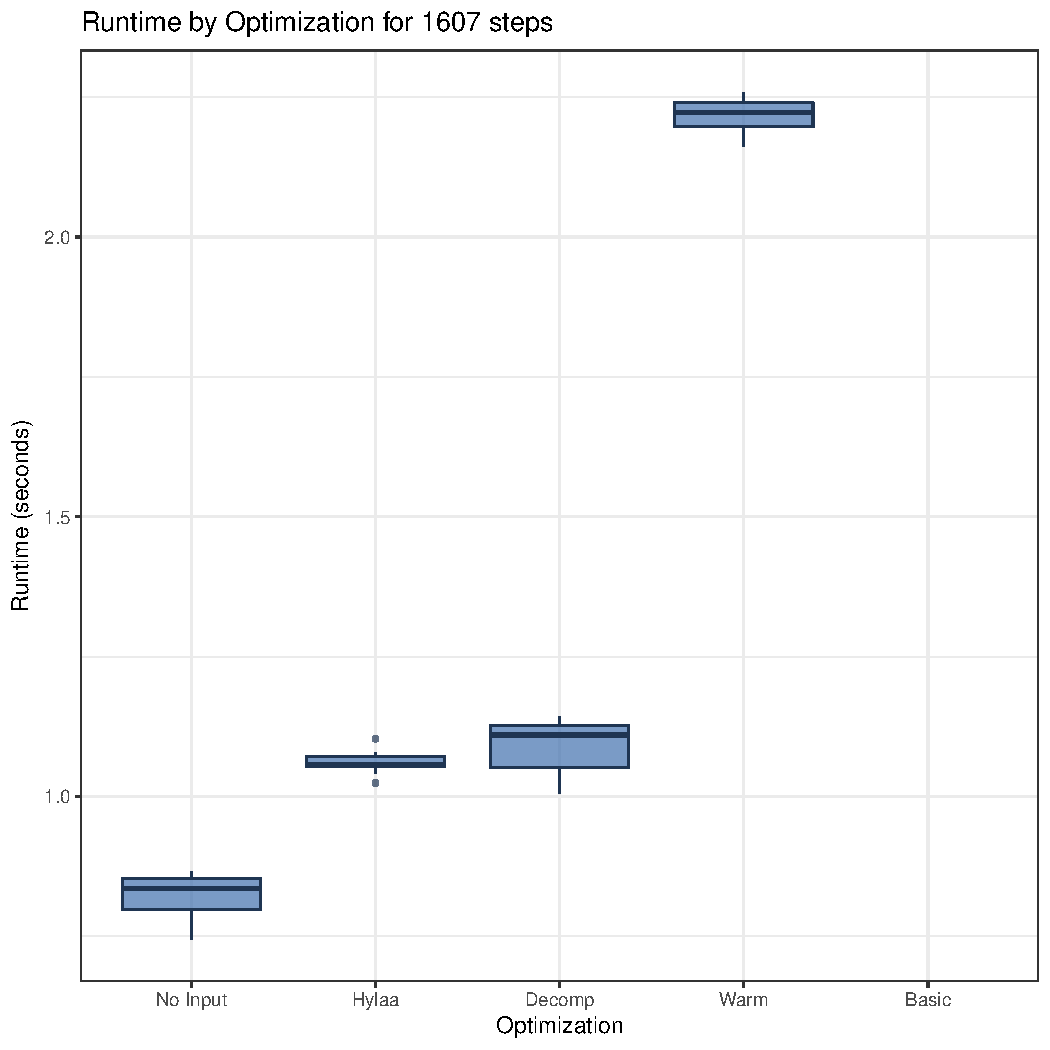
\includegraphics[width=\maxwidth]{figure/steps1607-1} 

\end{knitrout}
\subsubsection{Overview for 2089 steps}
\begin{knitrout}
\definecolor{shadecolor}{rgb}{0.969, 0.969, 0.969}\color{fgcolor}
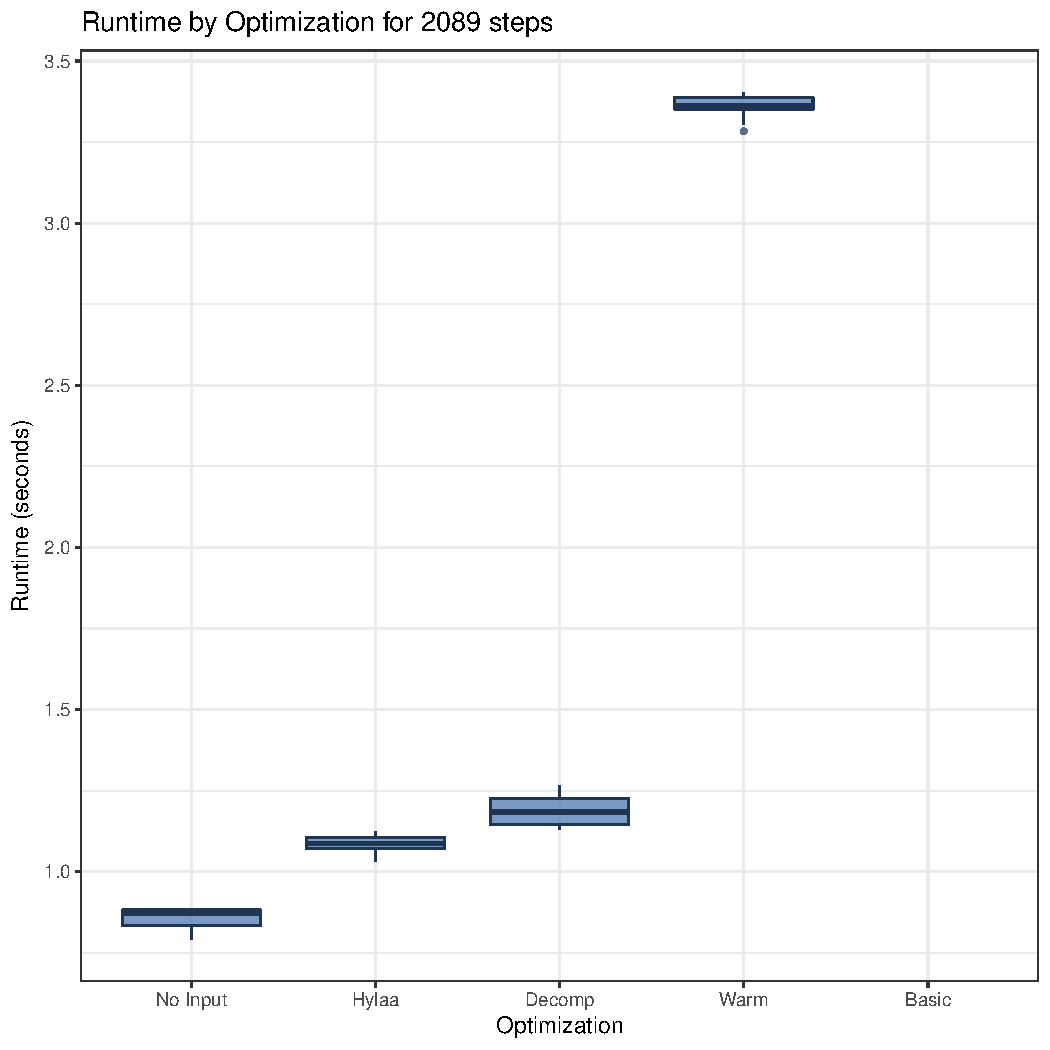
\includegraphics[width=\maxwidth]{figure/steps2089-1} 

\end{knitrout}
\subsubsection{Overview for 2716 steps}
\begin{knitrout}
\definecolor{shadecolor}{rgb}{0.969, 0.969, 0.969}\color{fgcolor}
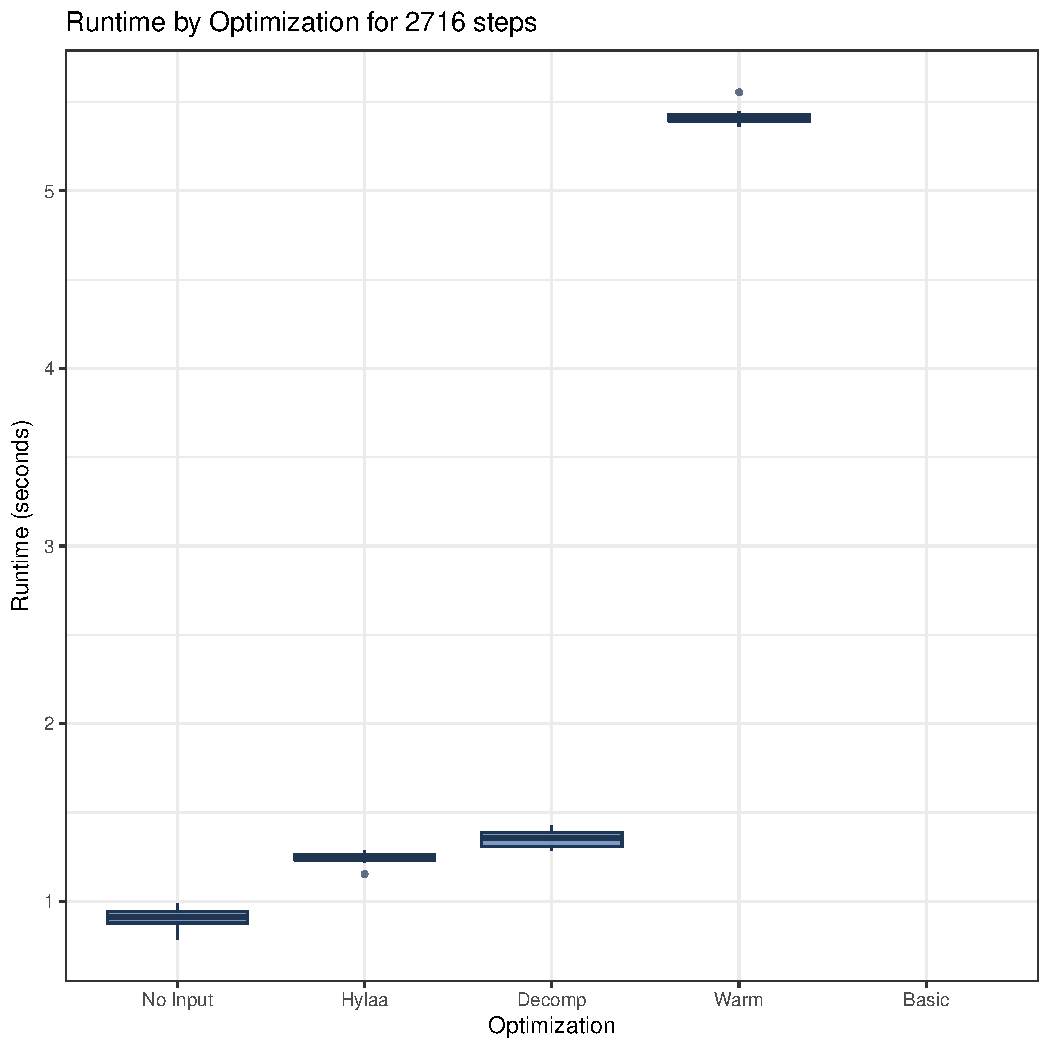
\includegraphics[width=\maxwidth]{figure/steps2716-1} 

\end{knitrout}
\subsubsection{Overview for 3531 steps}
\begin{knitrout}
\definecolor{shadecolor}{rgb}{0.969, 0.969, 0.969}\color{fgcolor}
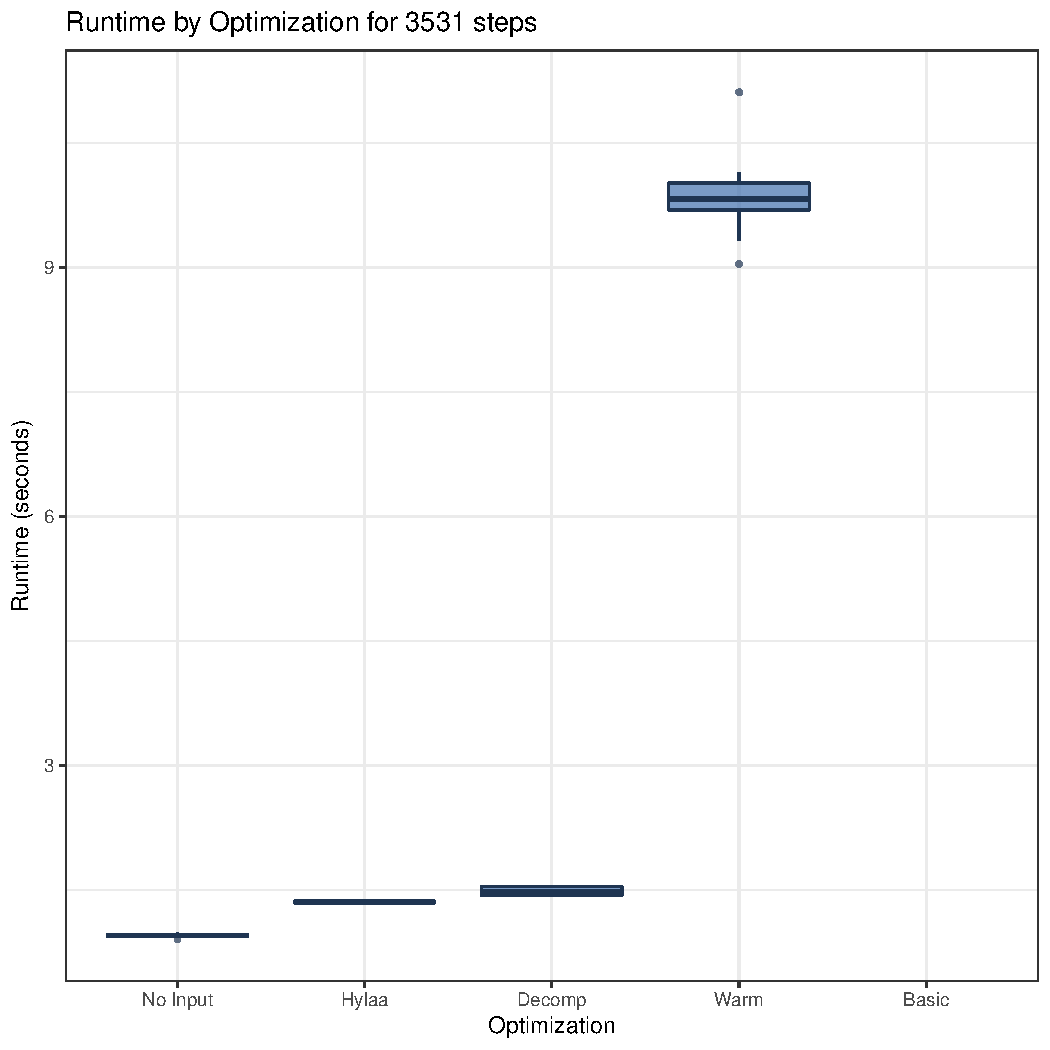
\includegraphics[width=\maxwidth]{figure/steps3531-1} 

\end{knitrout}
\subsubsection{Overview for 4590 steps}
\begin{knitrout}
\definecolor{shadecolor}{rgb}{0.969, 0.969, 0.969}\color{fgcolor}
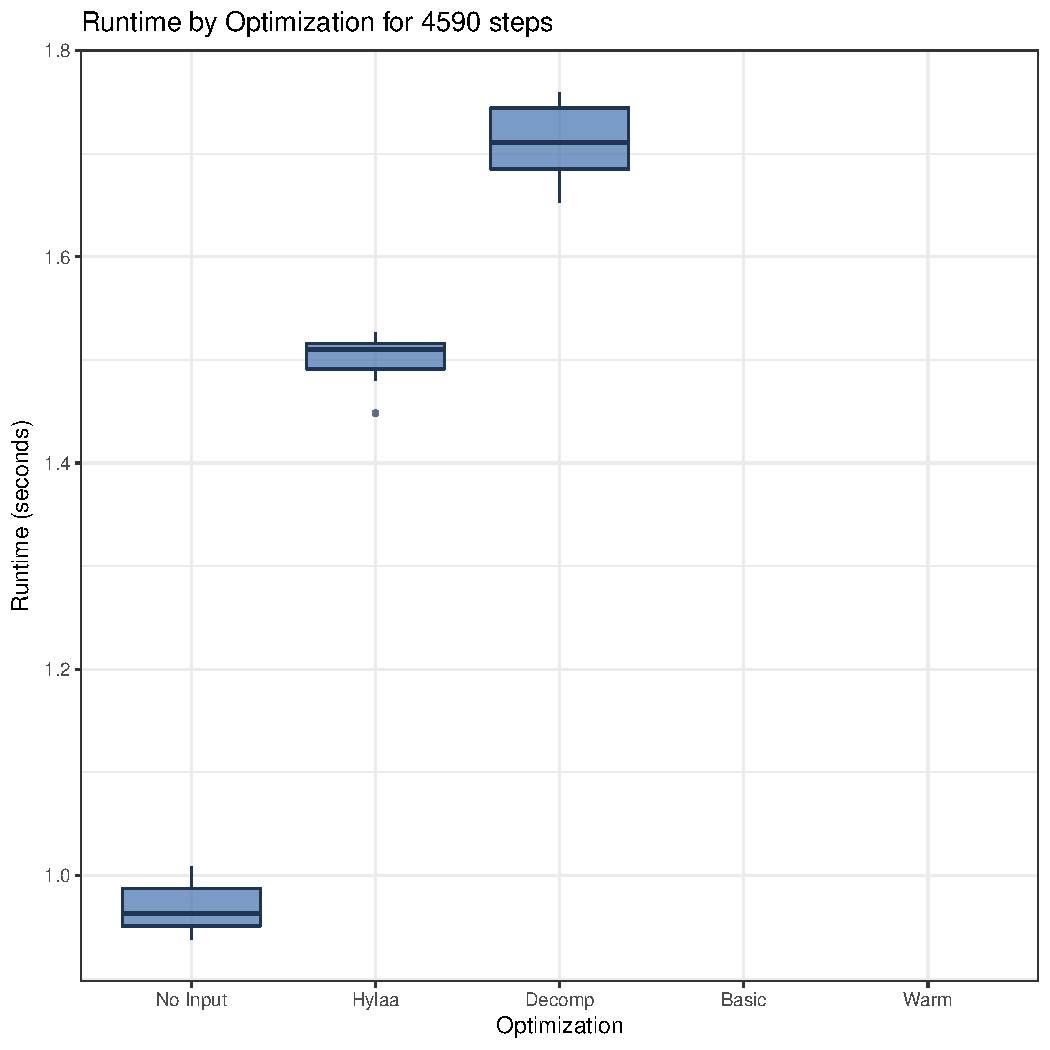
\includegraphics[width=\maxwidth]{figure/steps4590-1} 

\end{knitrout}
\subsubsection{Overview for 5967 steps}
\begin{knitrout}
\definecolor{shadecolor}{rgb}{0.969, 0.969, 0.969}\color{fgcolor}
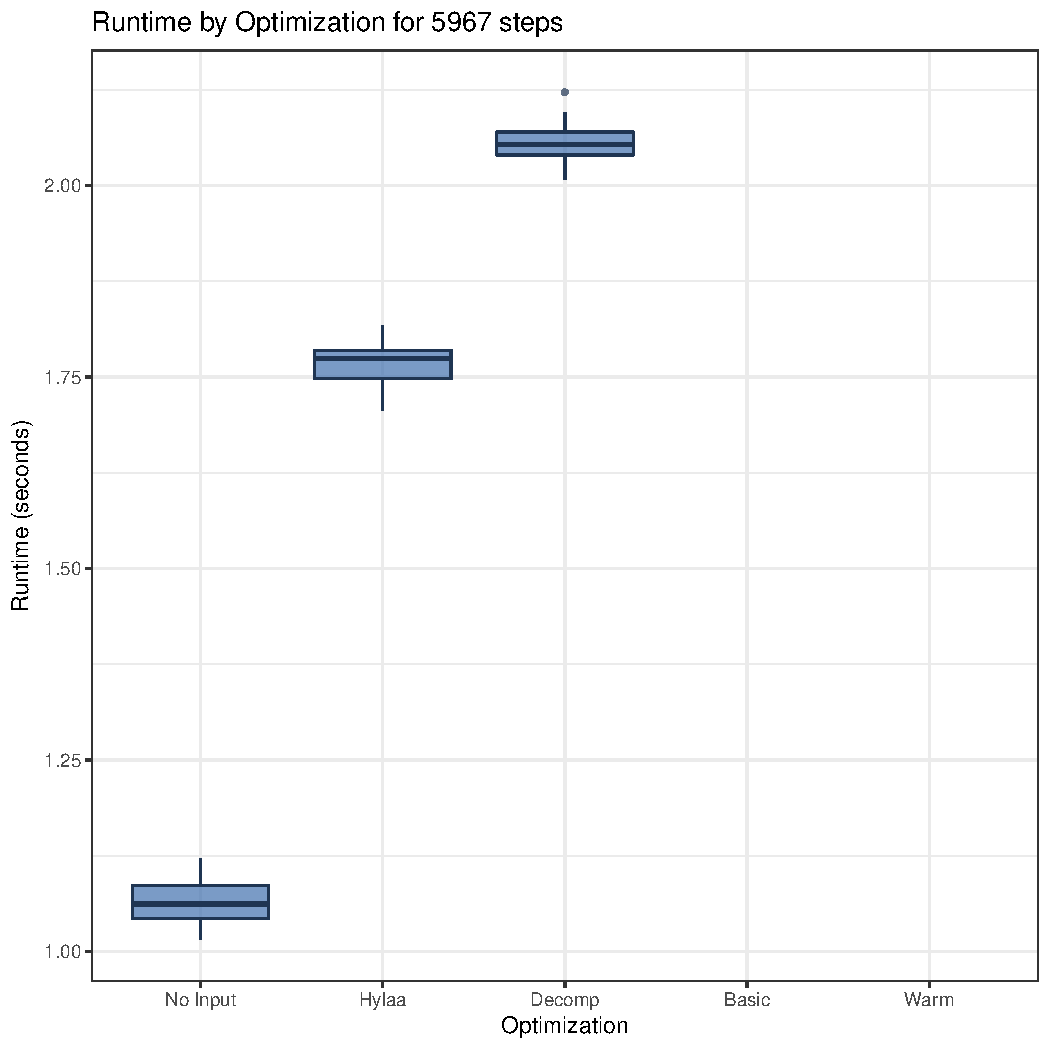
\includegraphics[width=\maxwidth]{figure/steps5967-1} 

\end{knitrout}
\subsubsection{Overview for 7757 steps}
\begin{knitrout}
\definecolor{shadecolor}{rgb}{0.969, 0.969, 0.969}\color{fgcolor}
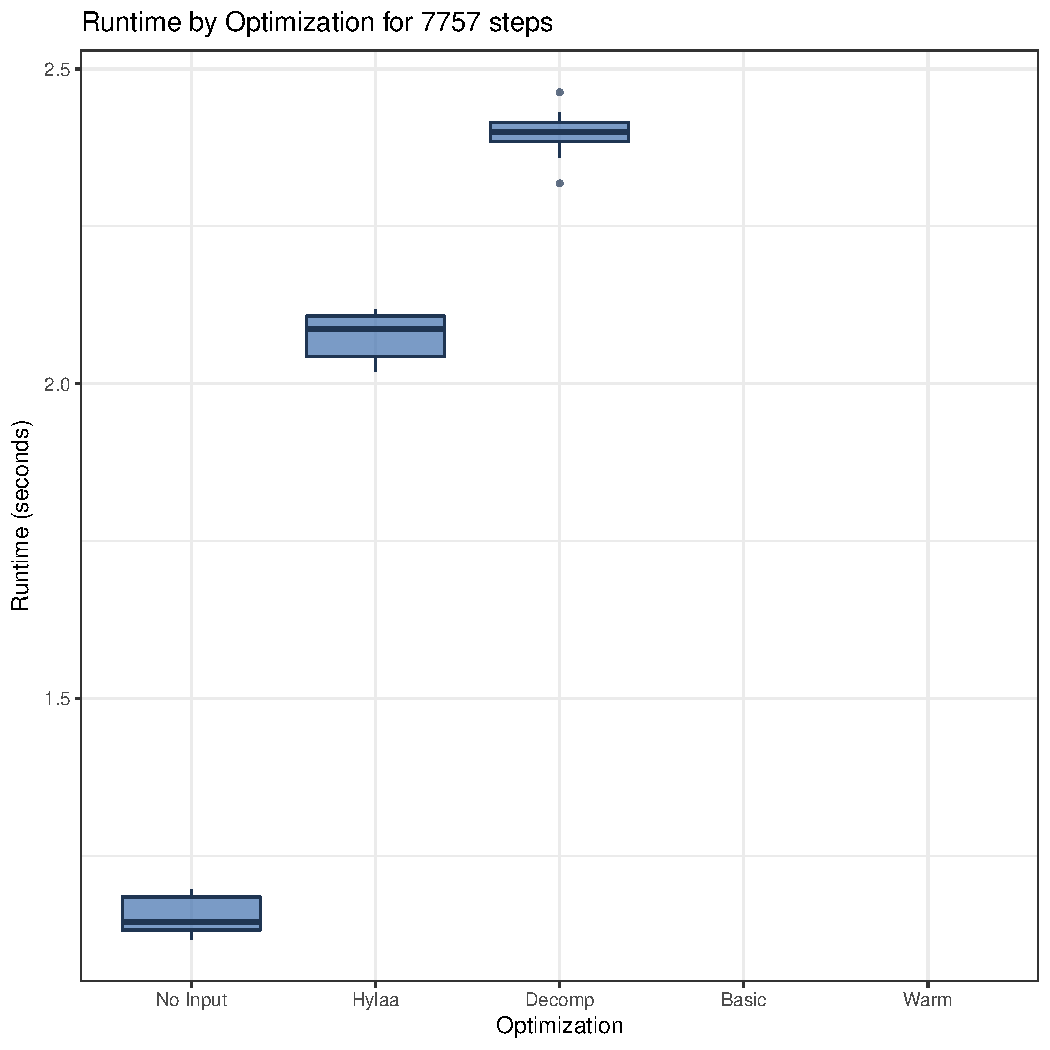
\includegraphics[width=\maxwidth]{figure/steps7757-1} 

\end{knitrout}
\subsubsection{Overview for 10085 steps}
\begin{knitrout}
\definecolor{shadecolor}{rgb}{0.969, 0.969, 0.969}\color{fgcolor}
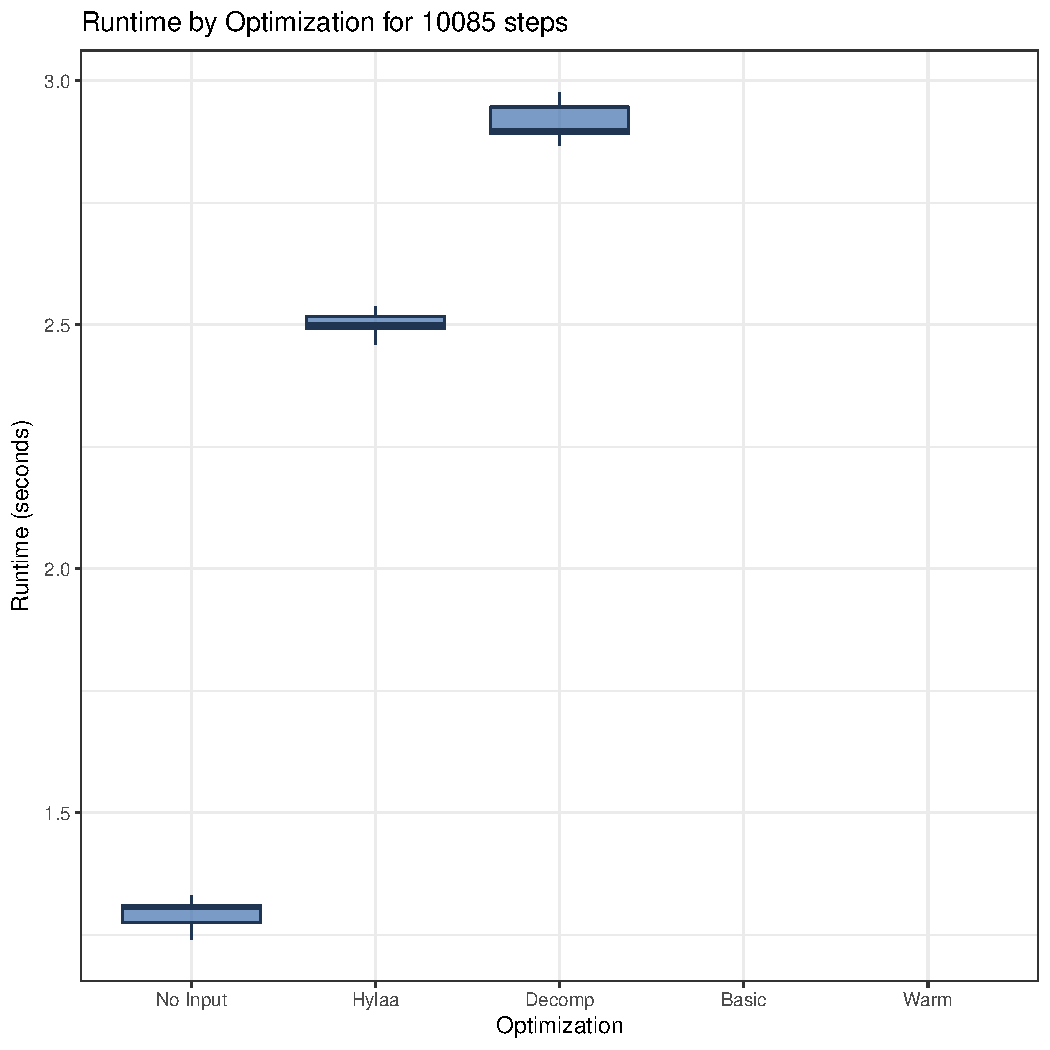
\includegraphics[width=\maxwidth]{figure/steps10085-1} 

\end{knitrout}
\subsubsection{Overview for 13110 steps}
\begin{knitrout}
\definecolor{shadecolor}{rgb}{0.969, 0.969, 0.969}\color{fgcolor}
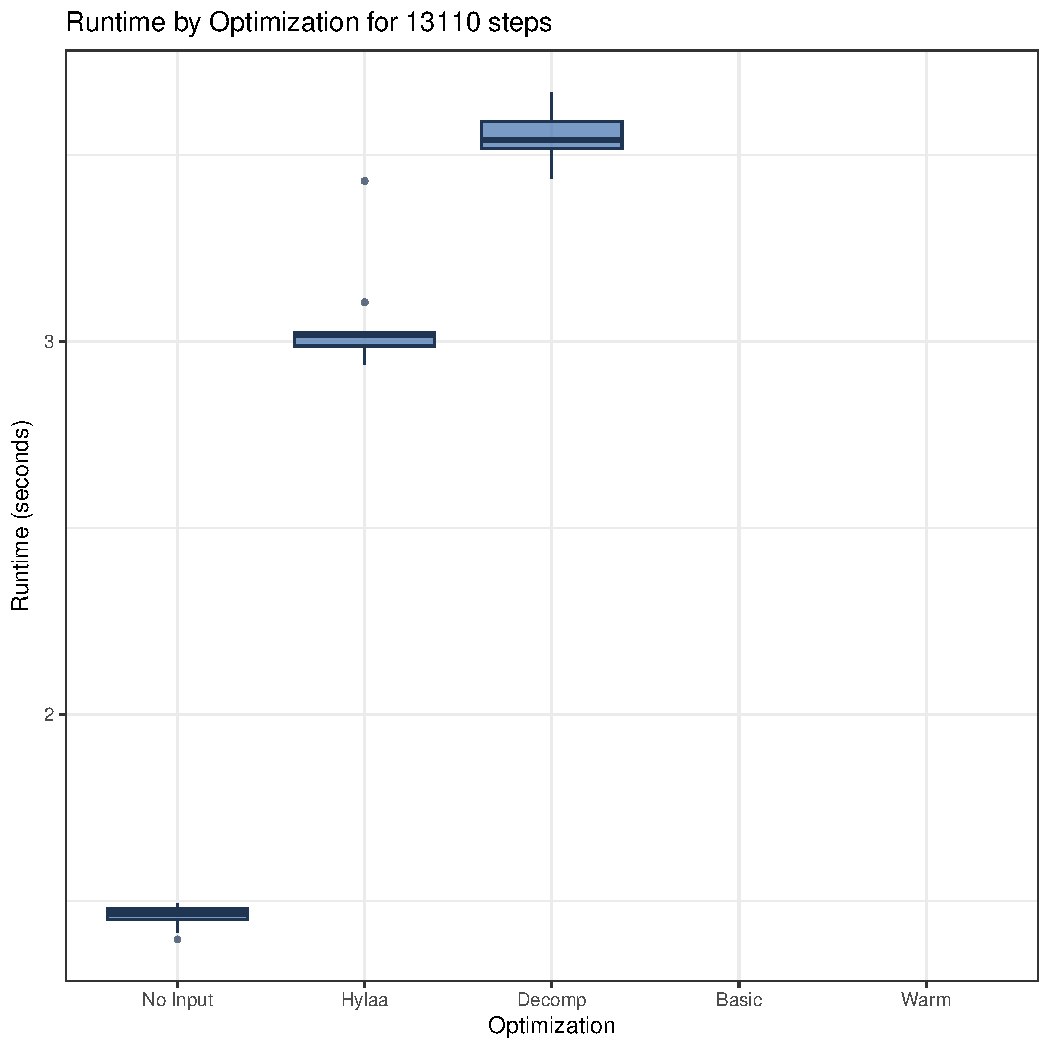
\includegraphics[width=\maxwidth]{figure/steps13110-1} 

\end{knitrout}
\subsubsection{Overview for 17043 steps}
\begin{knitrout}
\definecolor{shadecolor}{rgb}{0.969, 0.969, 0.969}\color{fgcolor}
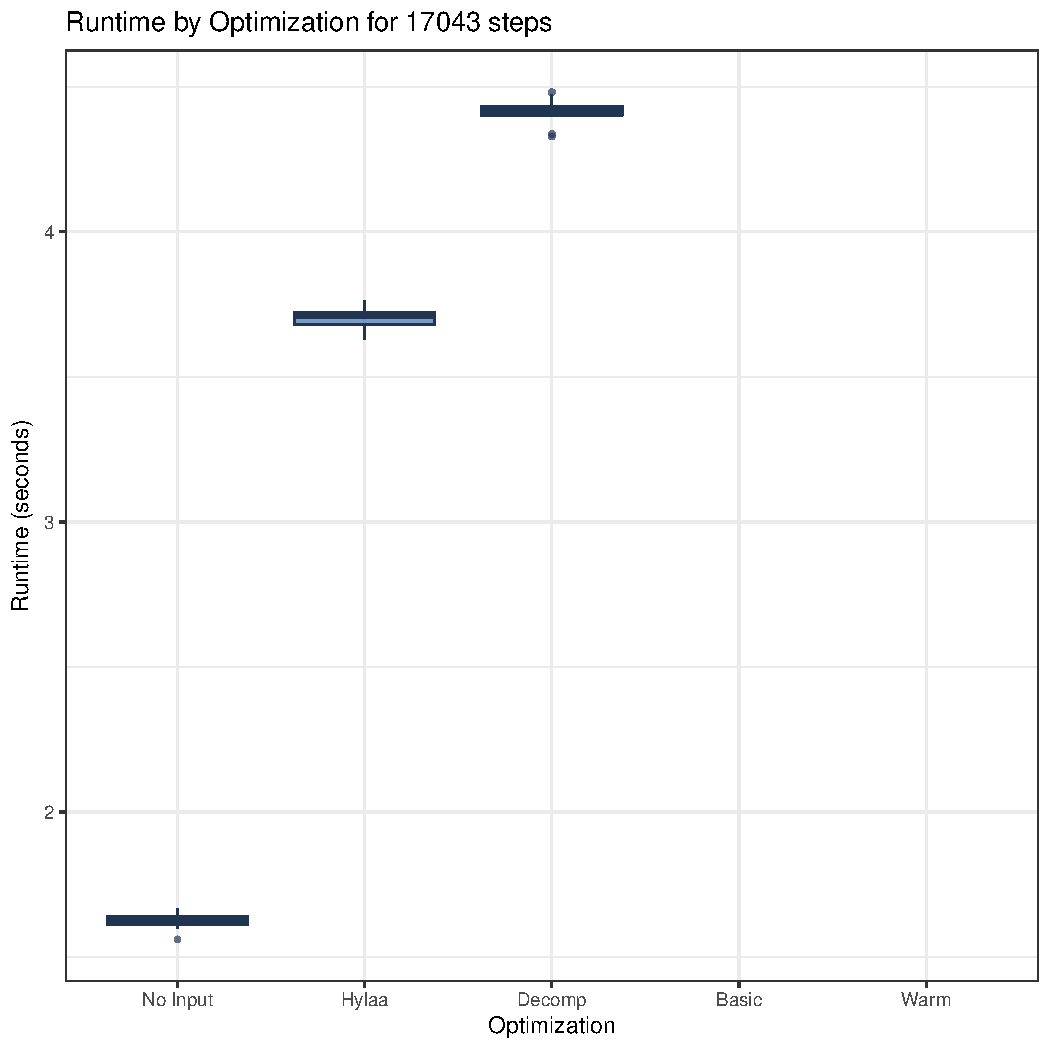
\includegraphics[width=\maxwidth]{figure/steps17043-1} 

\end{knitrout}
\subsubsection{Overview for 22157 steps}
\begin{knitrout}
\definecolor{shadecolor}{rgb}{0.969, 0.969, 0.969}\color{fgcolor}
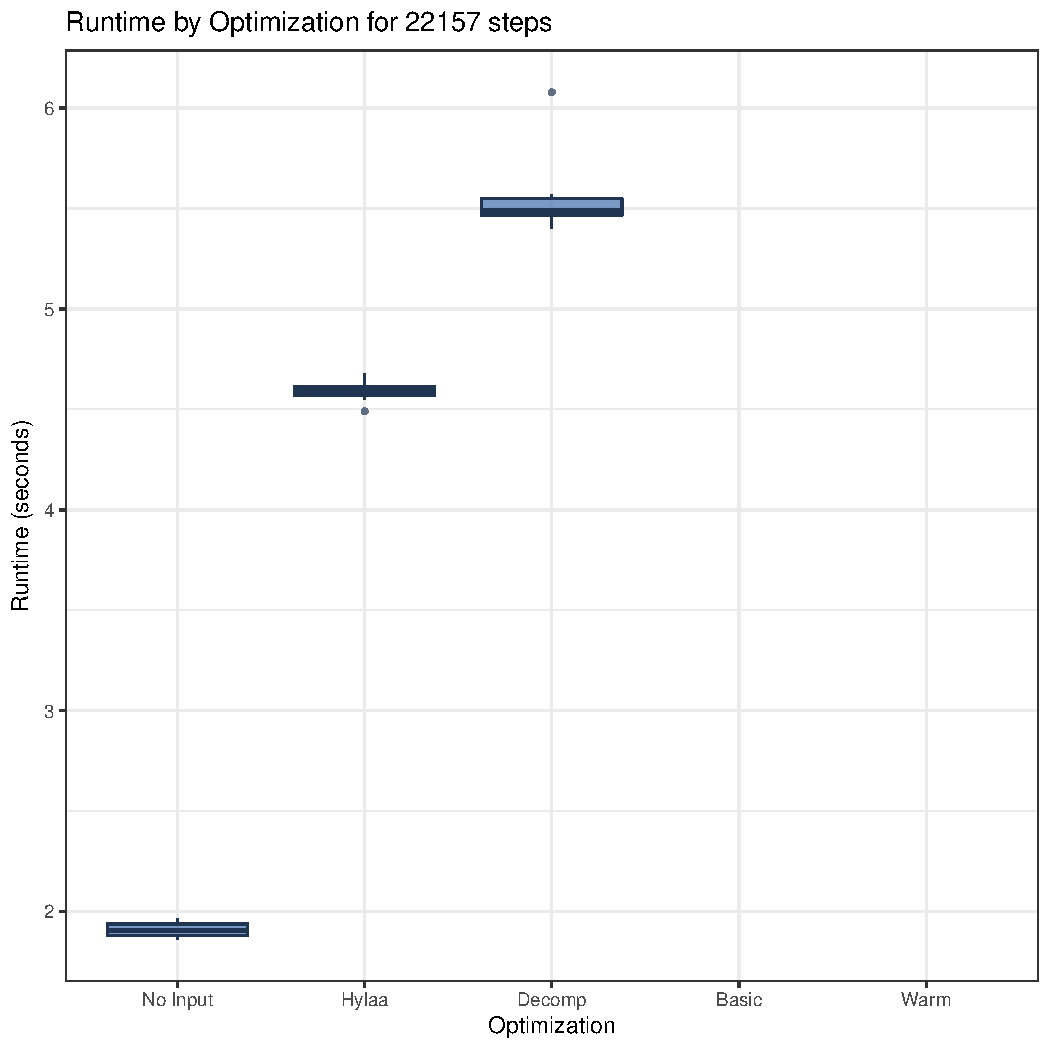
\includegraphics[width=\maxwidth]{figure/steps22157-1} 

\end{knitrout}
\subsubsection{Overview for 28804 steps}
\begin{knitrout}
\definecolor{shadecolor}{rgb}{0.969, 0.969, 0.969}\color{fgcolor}
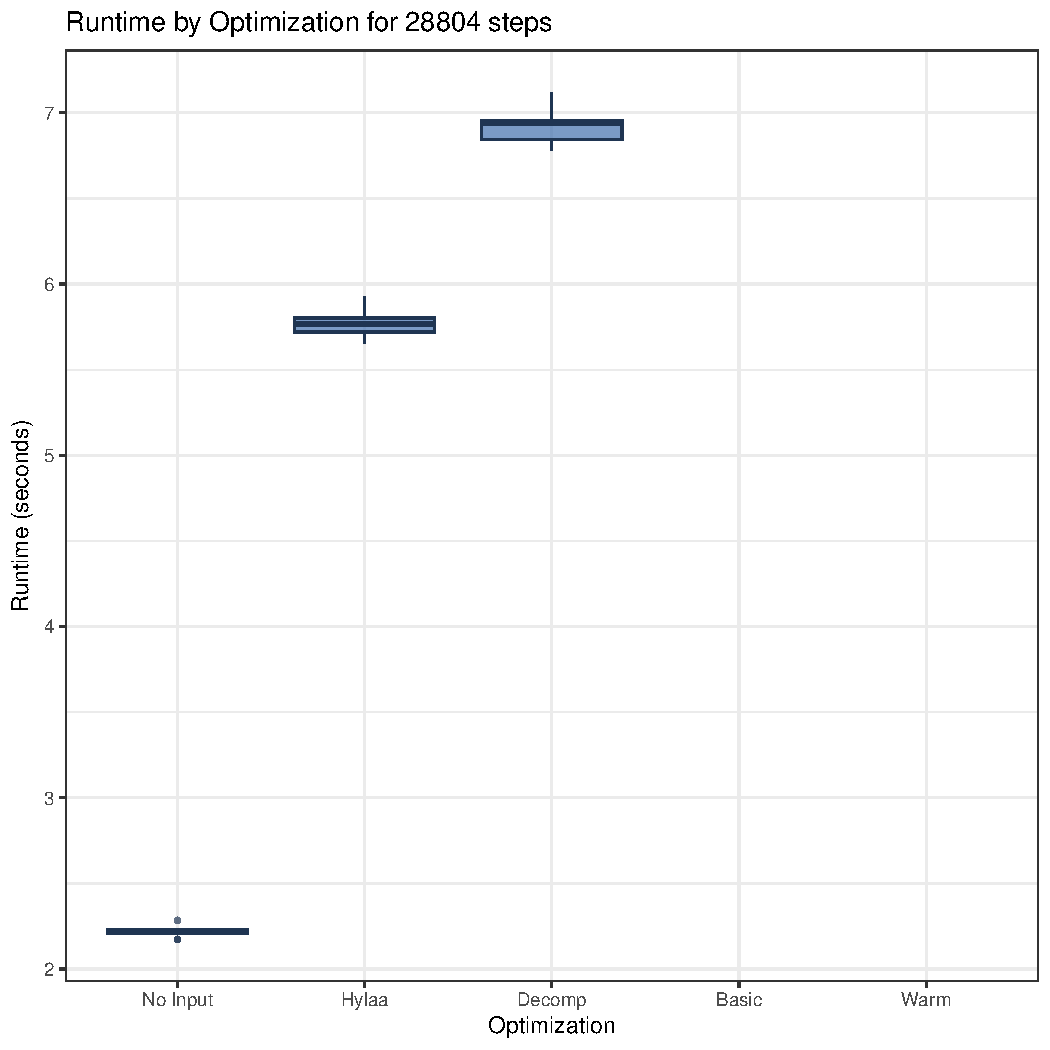
\includegraphics[width=\maxwidth]{figure/steps28804-1} 

\end{knitrout}
\subsubsection{Overview for 37445 steps}
\begin{knitrout}
\definecolor{shadecolor}{rgb}{0.969, 0.969, 0.969}\color{fgcolor}
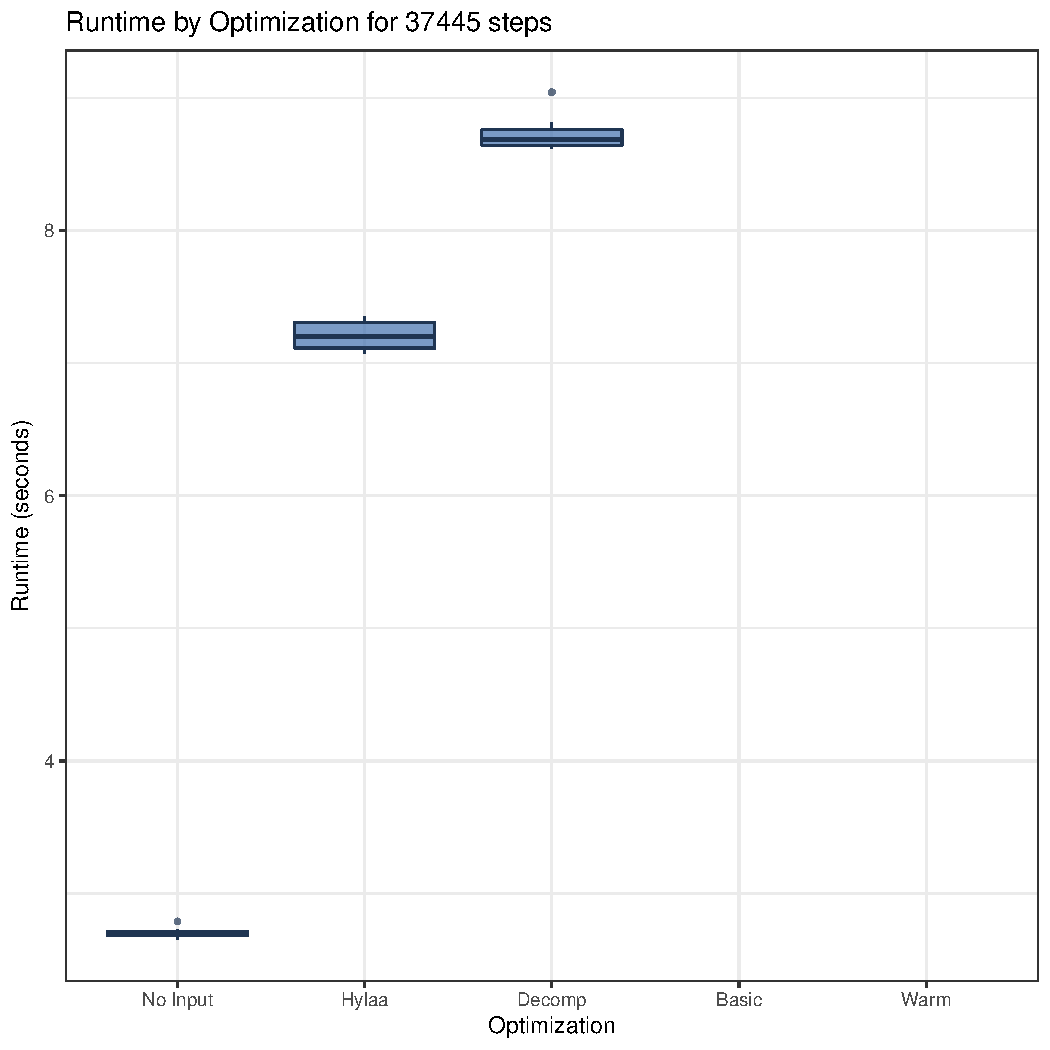
\includegraphics[width=\maxwidth]{figure/steps37445-1} 

\end{knitrout}
\subsubsection{Overview for 48679 steps}
\begin{knitrout}
\definecolor{shadecolor}{rgb}{0.969, 0.969, 0.969}\color{fgcolor}
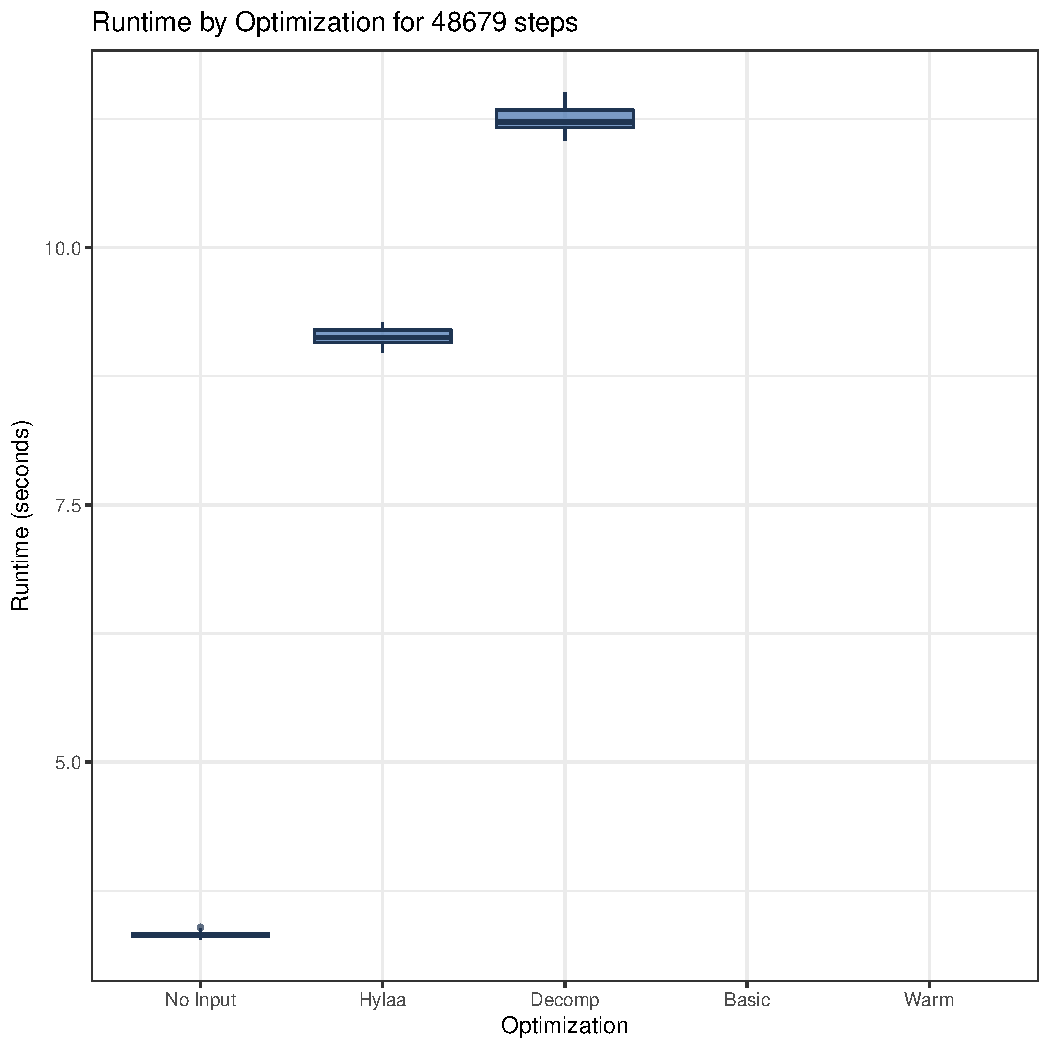
\includegraphics[width=\maxwidth]{figure/steps48679-1} 

\end{knitrout}
\subsubsection{Overview for 63282 steps}
\begin{knitrout}
\definecolor{shadecolor}{rgb}{0.969, 0.969, 0.969}\color{fgcolor}
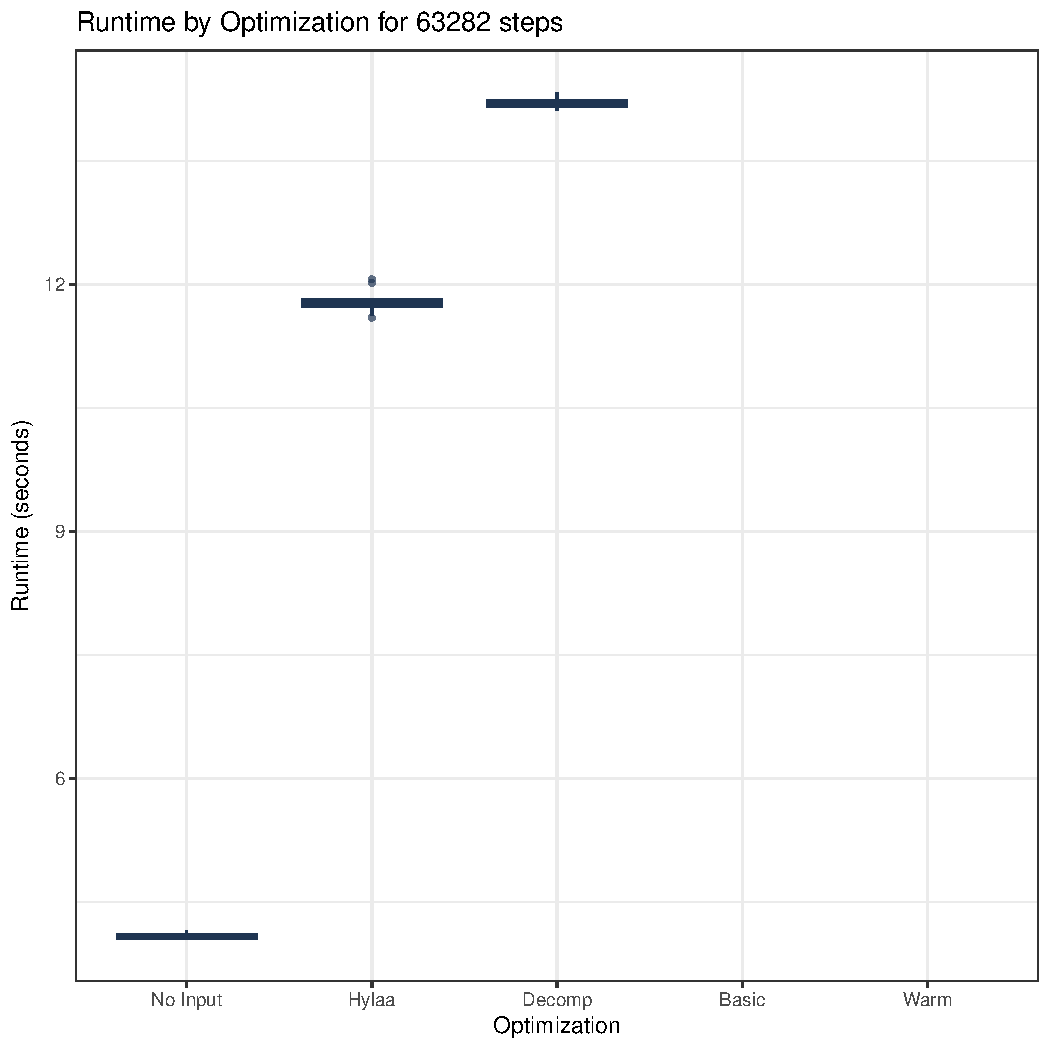
\includegraphics[width=\maxwidth]{figure/steps63282-1} 

\end{knitrout}
\subsubsection{Overview for 82267 steps}
\begin{knitrout}
\definecolor{shadecolor}{rgb}{0.969, 0.969, 0.969}\color{fgcolor}
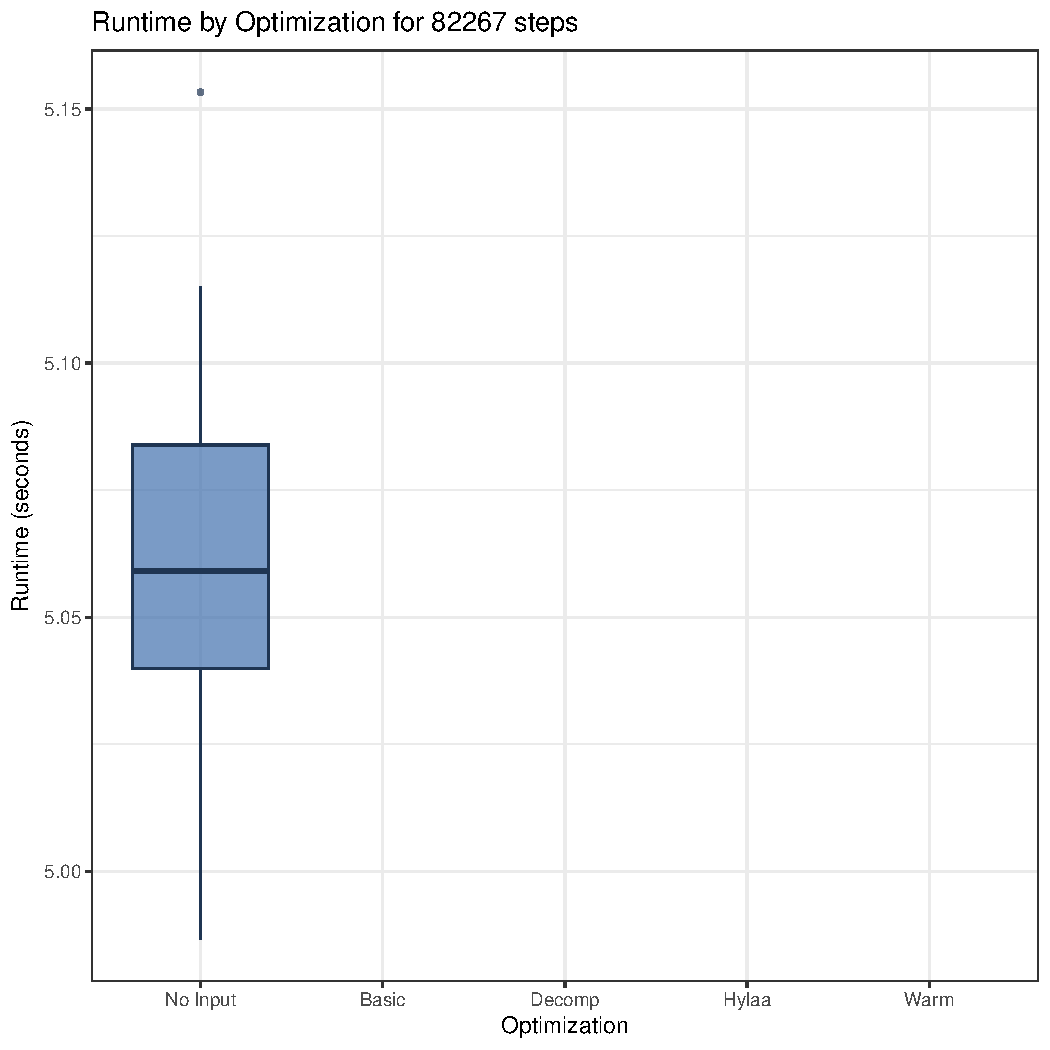
\includegraphics[width=\maxwidth]{figure/steps82267-1} 

\end{knitrout}
\subsubsection{Overview for 106948 steps}
\begin{knitrout}
\definecolor{shadecolor}{rgb}{0.969, 0.969, 0.969}\color{fgcolor}
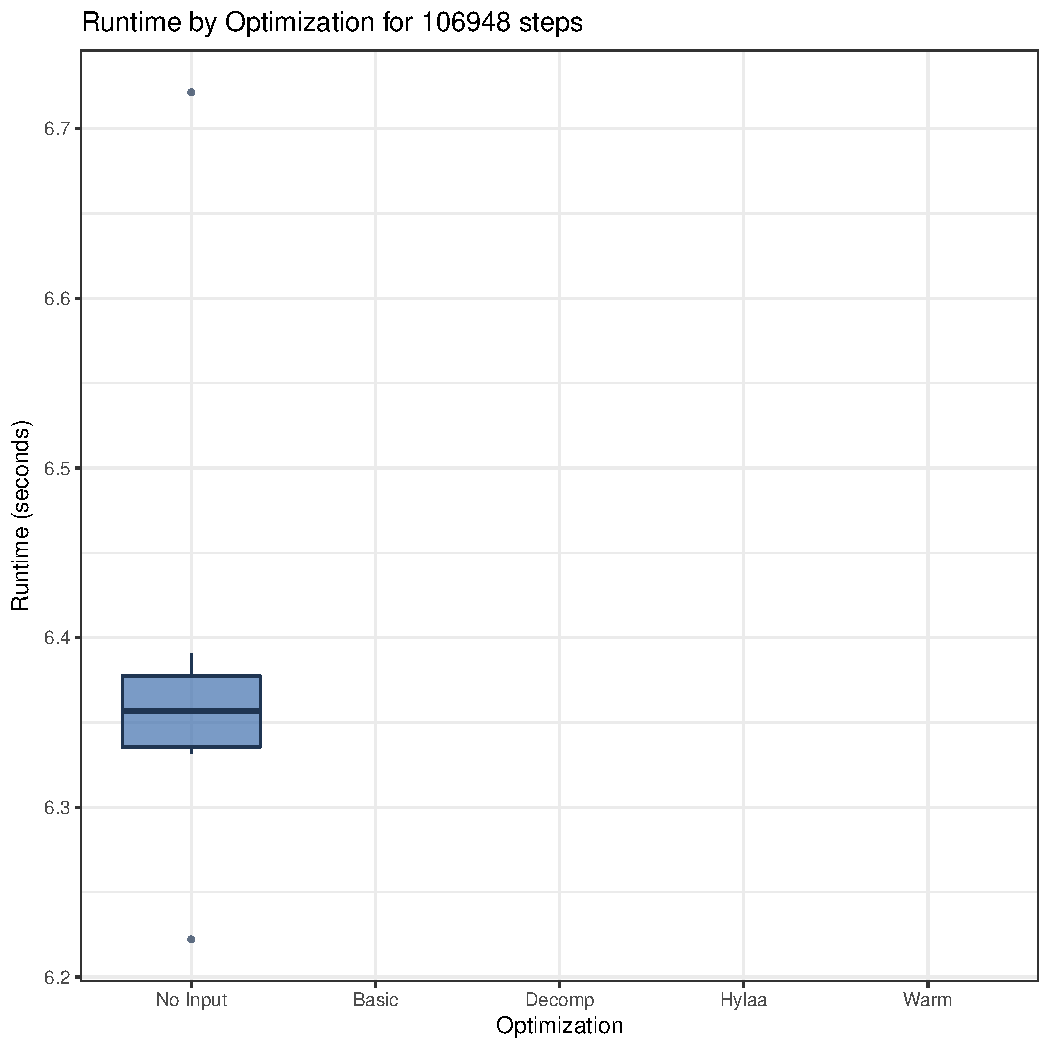
\includegraphics[width=\maxwidth]{figure/steps106948-1} 

\end{knitrout}
\subsubsection{Overview for 139032 steps}
\begin{knitrout}
\definecolor{shadecolor}{rgb}{0.969, 0.969, 0.969}\color{fgcolor}
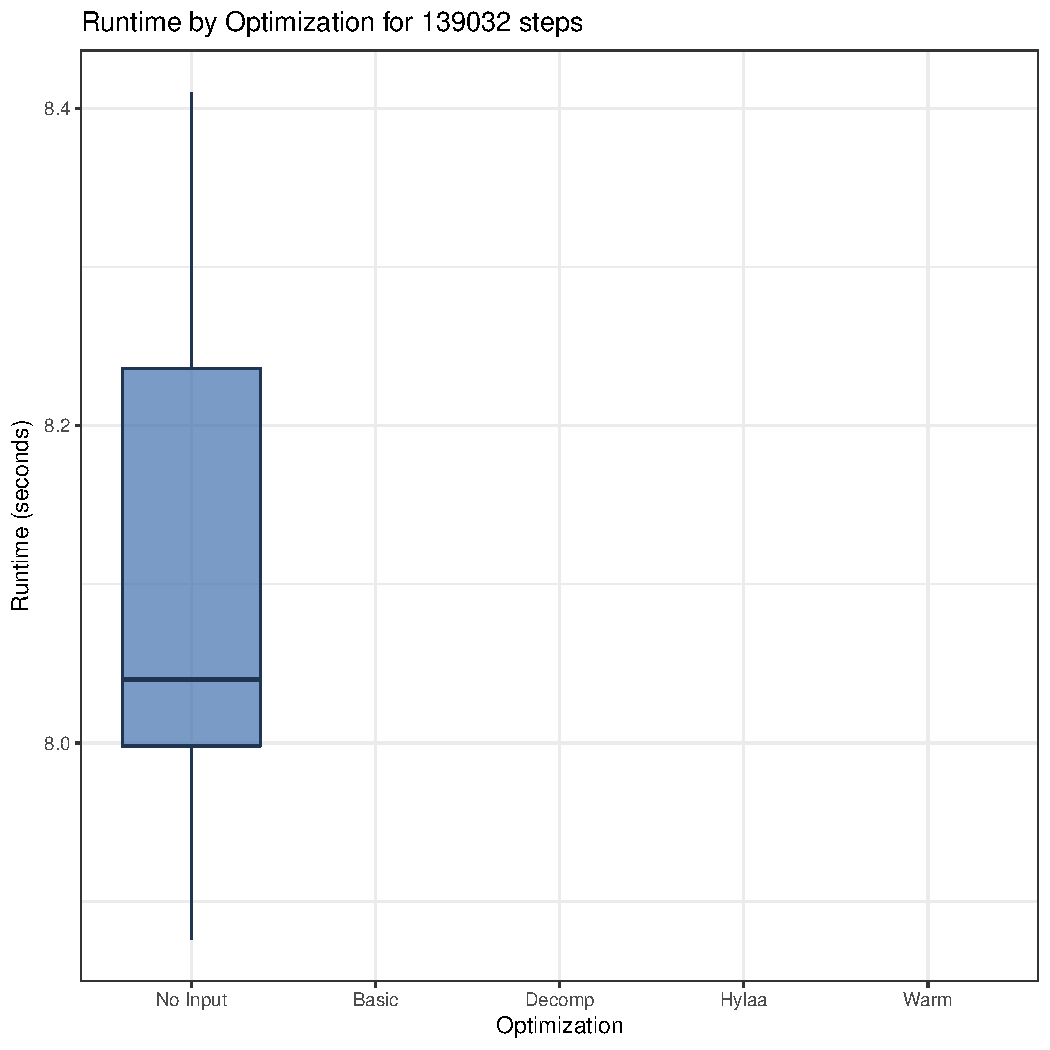
\includegraphics[width=\maxwidth]{figure/steps139032-1} 

\end{knitrout}
\subsubsection{Overview for 180742 steps}
\begin{knitrout}
\definecolor{shadecolor}{rgb}{0.969, 0.969, 0.969}\color{fgcolor}
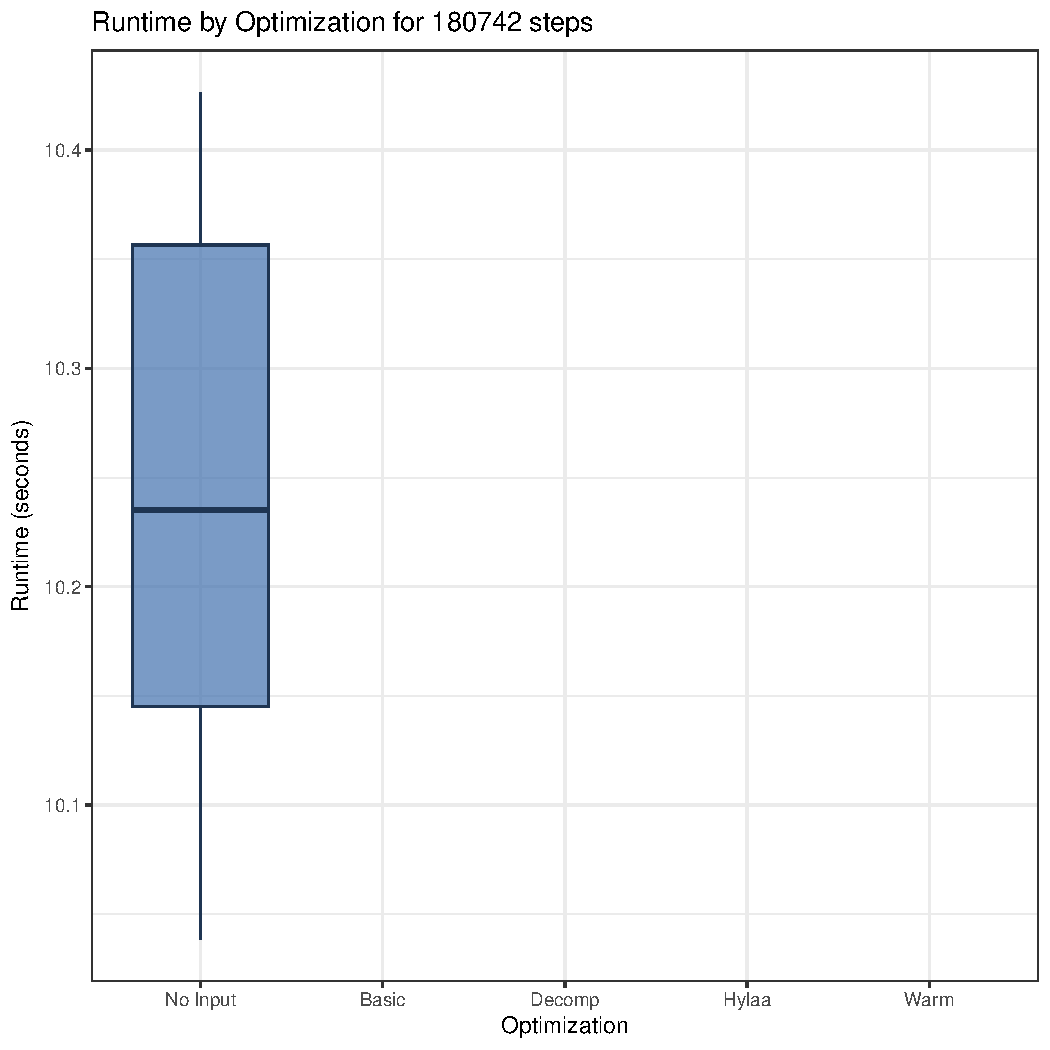
\includegraphics[width=\maxwidth]{figure/steps180742-1} 

\end{knitrout}

\section{Research Hypotheses}

\subsection{RH1: Runtime time for Hylaa is equals than runtime time for Warm}


 
\begin{knitrout}
\definecolor{shadecolor}{rgb}{0.969, 0.969, 0.969}\color{fgcolor}
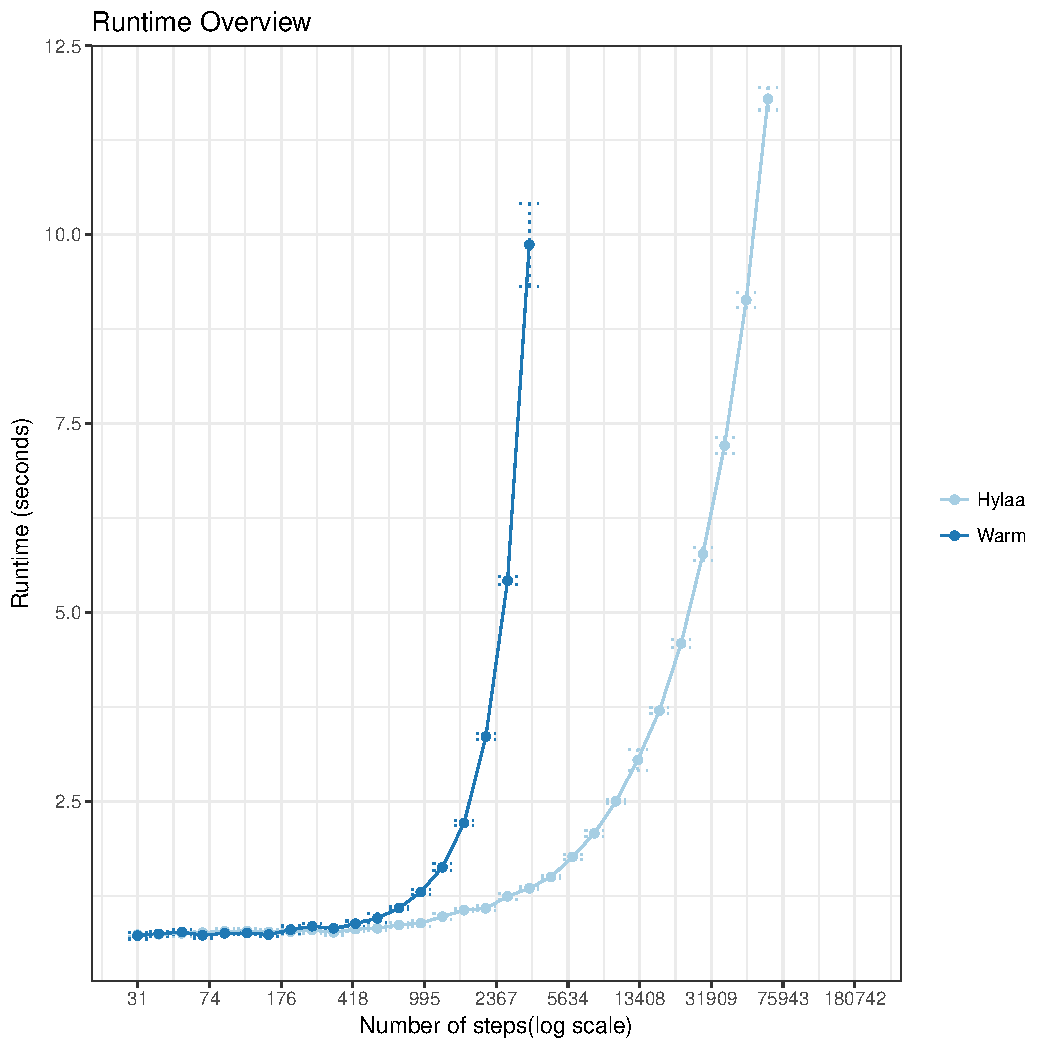
\includegraphics[width=\maxwidth]{figure/overview_RH1-1} 

\end{knitrout}
 	

\subsubsection{RH1.1: Object 31 steps}

 \textbf{Runtime for Hylaa}
\begin{knitrout}
\definecolor{shadecolor}{rgb}{0.969, 0.969, 0.969}\color{fgcolor}\begin{kframe}
\begin{verbatim}
## [1] "Sample size:  10"
##    Min. 1st Qu.  Median    Mean 3rd Qu.    Max. 
##  0.6929  0.7270  0.7402  0.7371  0.7560  0.7729
\end{verbatim}
\end{kframe}
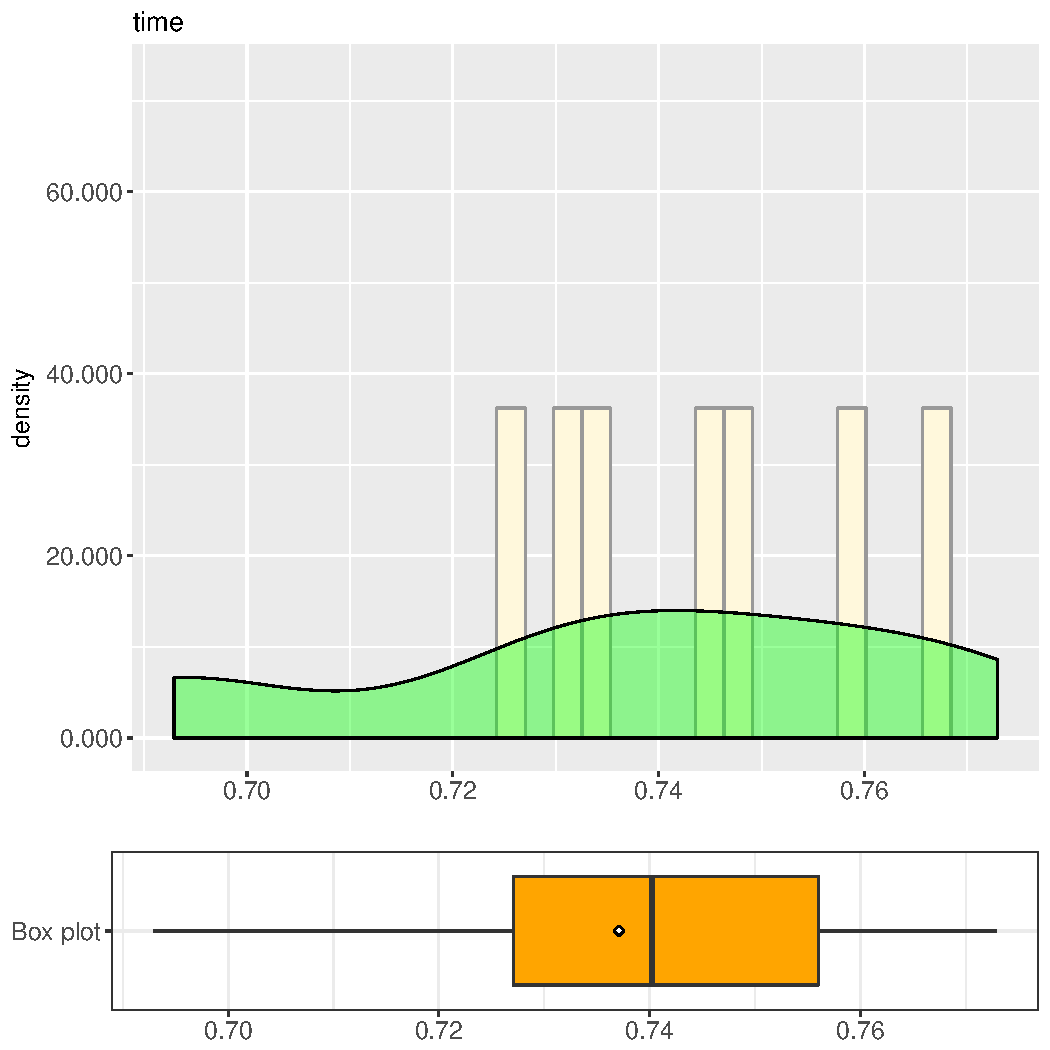
\includegraphics[width=\maxwidth]{figure/RH1_Hylaa_steps31-1} 
\begin{kframe}\begin{verbatim}
## 
## 	Shapiro-Wilk normality test
## 
## data:  subset(json_data, treatment == "Hylaa" & object == "steps31")$time
## W = 0.92348, p-value = 0.3869
## 
## [1] "Shapiro test: Null Hypothesis (normality) not rejected. P-value: 0.386919454155626"
\end{verbatim}
\end{kframe}
\end{knitrout}
 \textbf{Runtime for Warm}
\begin{knitrout}
\definecolor{shadecolor}{rgb}{0.969, 0.969, 0.969}\color{fgcolor}\begin{kframe}
\begin{verbatim}
## [1] "Sample size:  10"
##    Min. 1st Qu.  Median    Mean 3rd Qu.    Max. 
##  0.6628  0.6856  0.7329  0.7237  0.7640  0.7709
\end{verbatim}
\end{kframe}
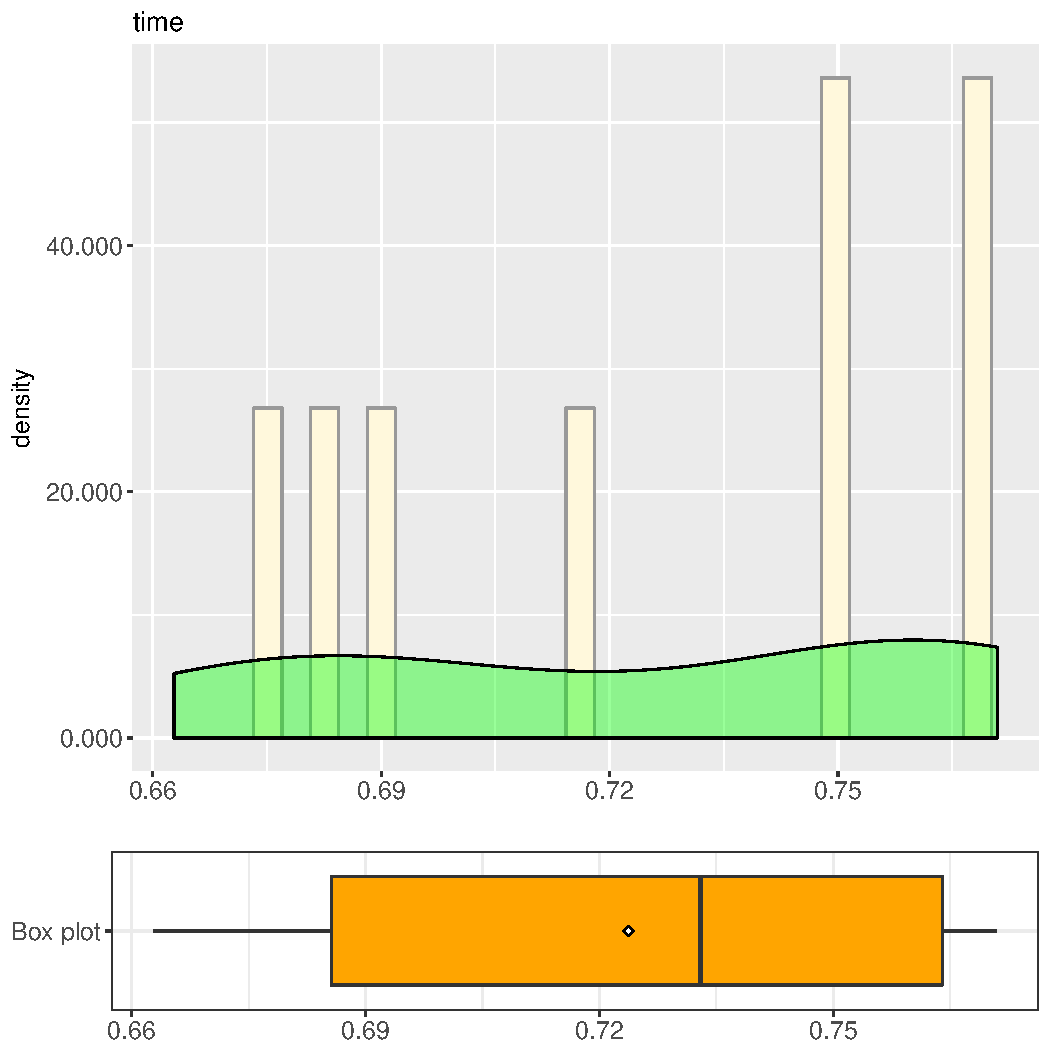
\includegraphics[width=\maxwidth]{figure/RH1_Warm_steps31-1} 
\begin{kframe}\begin{verbatim}
## 
## 	Shapiro-Wilk normality test
## 
## data:  subset(json_data, treatment == "Warm" & object == "steps31")$time
## W = 0.86528, p-value = 0.08804
## 
## [1] "Shapiro test: Null Hypothesis (normality) not rejected. P-value: 0.0880390766774588"
\end{verbatim}
\end{kframe}
\end{knitrout}
  
 \textbf{Comparison}
  
\begin{knitrout}
\definecolor{shadecolor}{rgb}{0.969, 0.969, 0.969}\color{fgcolor}
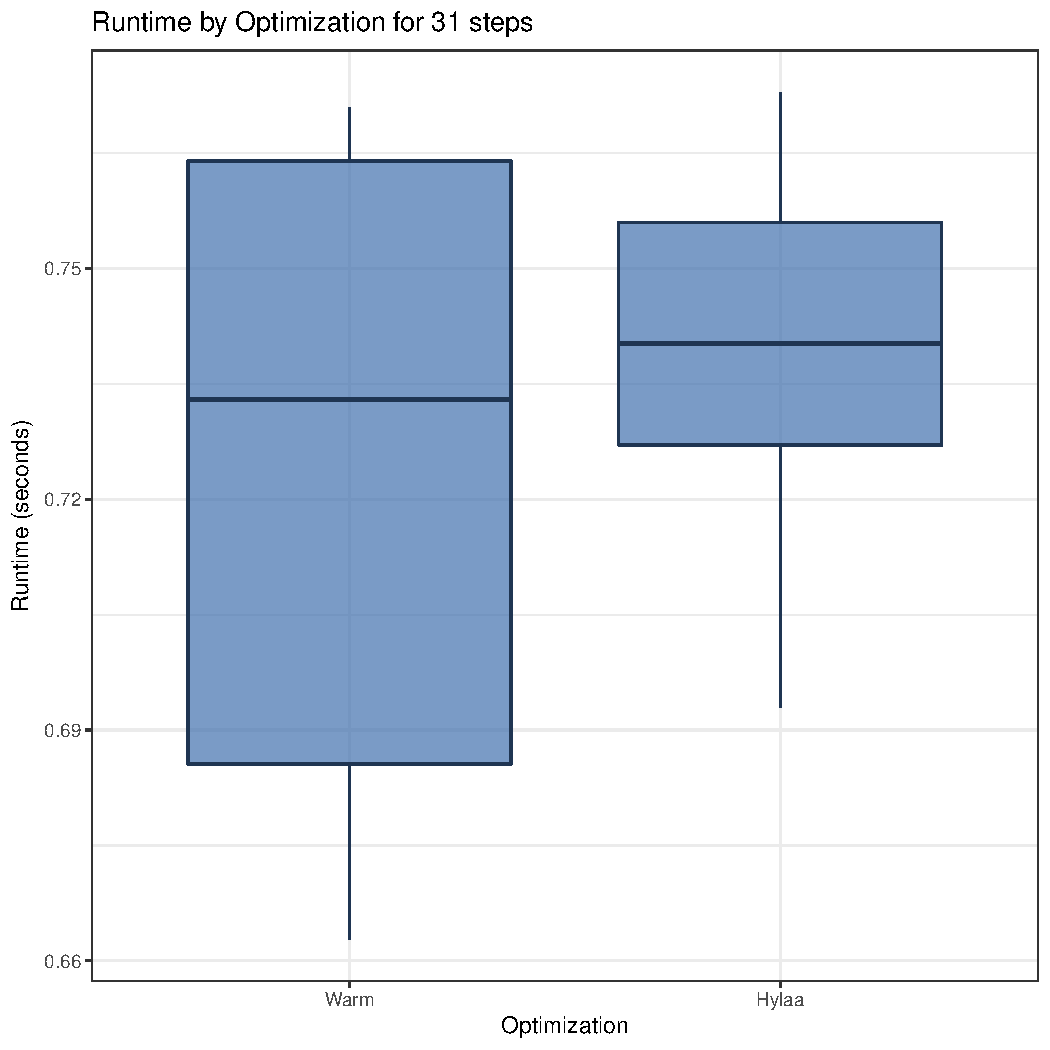
\includegraphics[width=\maxwidth]{figure/RH1_steps31-1} 
\begin{kframe}\begin{verbatim}
## [1] "Fisher's F-test to verify the homoskedasticity (homogeneity of variances)"
## 
## 	F test to compare two variances
## 
## data:  subset(json_data, treatment == "Hylaa" & object == "steps31")$time and subset(json_data, treatment == "Warm" & object == "steps31")$time
## F = 0.41659, num df = 9, denom df = 9, p-value = 0.2082
## alternative hypothesis: true ratio of variances is not equal to 1
## 95 percent confidence interval:
##  0.1034749 1.6771870
## sample estimates:
## ratio of variances 
##          0.4165895 
## 
## [1] "Homogeneity of variances: TRUE. P-value: 0.208187552120455"
## [1] "Assuming that the two samples are taken from populations that follow a Gaussian distribution (if we cannot assume that, we must solve this problem using the non-parametric test called Wilcoxon-Mann-Whitney test)"
## 
## 	Two Sample t-test
## 
## data:  subset(json_data, treatment == "Hylaa" & object == "steps31")$time and subset(json_data, treatment == "Warm" & object == "steps31")$time
## t = 0.82637, df = 18, p-value = 0.4194
## alternative hypothesis: true difference in means is not equal to 0
## 95 percent confidence interval:
##  -0.02062869  0.04737840
## sample estimates:
## mean of x mean of y 
## 0.7370949 0.7237201 
## 
## [1] "T-test: Null Hypothesis not rejected. P-value: 0.419413568997939"
## [1] ""
## [1] "Means comparison"
## [1] "Mean Runtime for Hylaa:  0.7370949268343"
## [1] "Mean Runtime for Warm:  0.7237200736998"
## [1] "Absolute difference:  0.0133748531345"
## Runtime for Hylaa is  1.8480699403742 % greater than 
##  Runtime for Warm
\end{verbatim}
\end{kframe}
\end{knitrout}


\subsubsection{RH1.2: Object 40 steps}

 \textbf{Runtime for Hylaa}
\begin{knitrout}
\definecolor{shadecolor}{rgb}{0.969, 0.969, 0.969}\color{fgcolor}\begin{kframe}
\begin{verbatim}
## [1] "Sample size:  10"
##    Min. 1st Qu.  Median    Mean 3rd Qu.    Max. 
##  0.7104  0.7190  0.7355  0.7432  0.7493  0.8064
\end{verbatim}
\end{kframe}
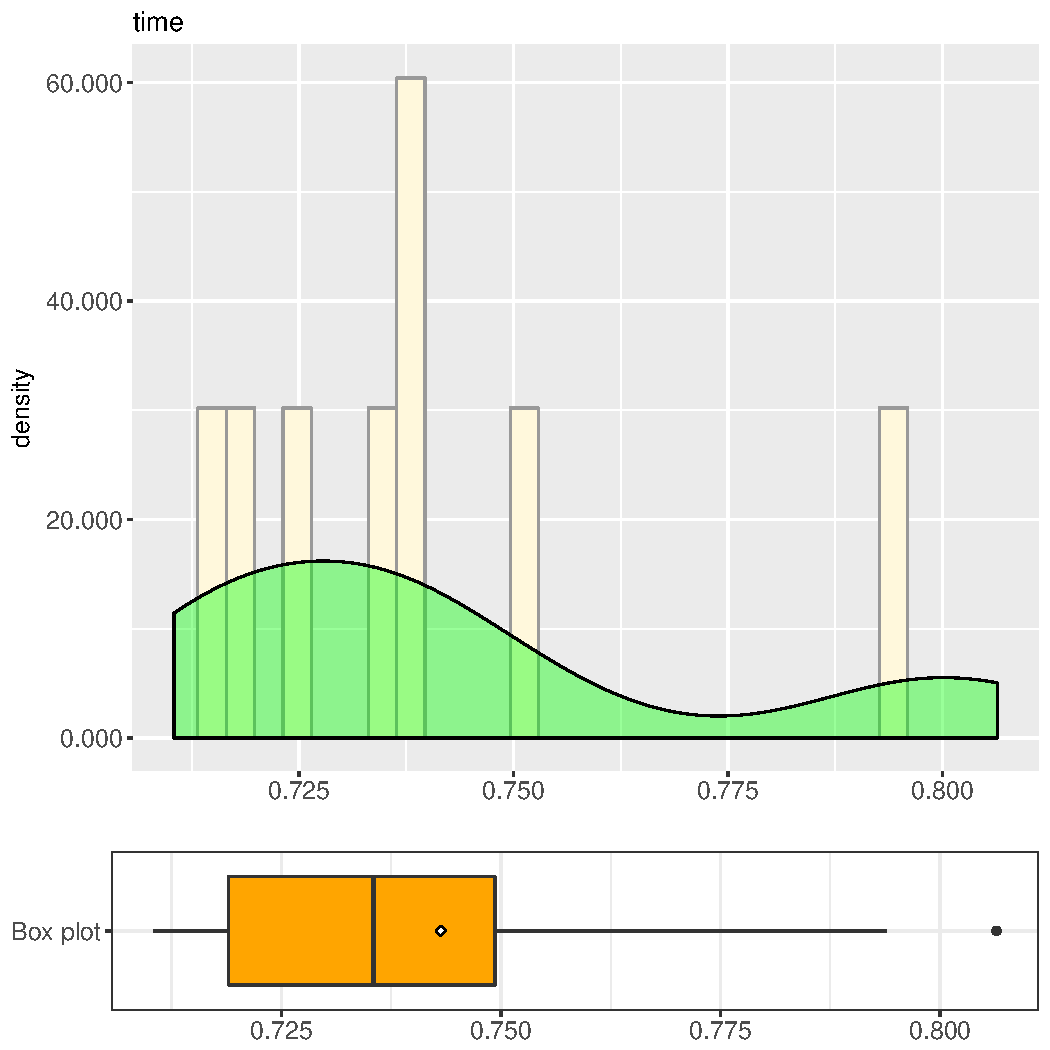
\includegraphics[width=\maxwidth]{figure/RH1_Hylaa_steps40-1} 
\begin{kframe}\begin{verbatim}
## 
## 	Shapiro-Wilk normality test
## 
## data:  subset(json_data, treatment == "Hylaa" & object == "steps40")$time
## W = 0.84556, p-value = 0.05142
## 
## [1] "Shapiro test: Null Hypothesis (normality) not rejected. P-value: 0.0514195741817329"
\end{verbatim}
\end{kframe}
\end{knitrout}
 \textbf{Runtime for Warm}
\begin{knitrout}
\definecolor{shadecolor}{rgb}{0.969, 0.969, 0.969}\color{fgcolor}\begin{kframe}
\begin{verbatim}
## [1] "Sample size:  10"
##    Min. 1st Qu.  Median    Mean 3rd Qu.    Max. 
##  0.6924  0.7288  0.7488  0.7476  0.7711  0.8021
\end{verbatim}
\end{kframe}
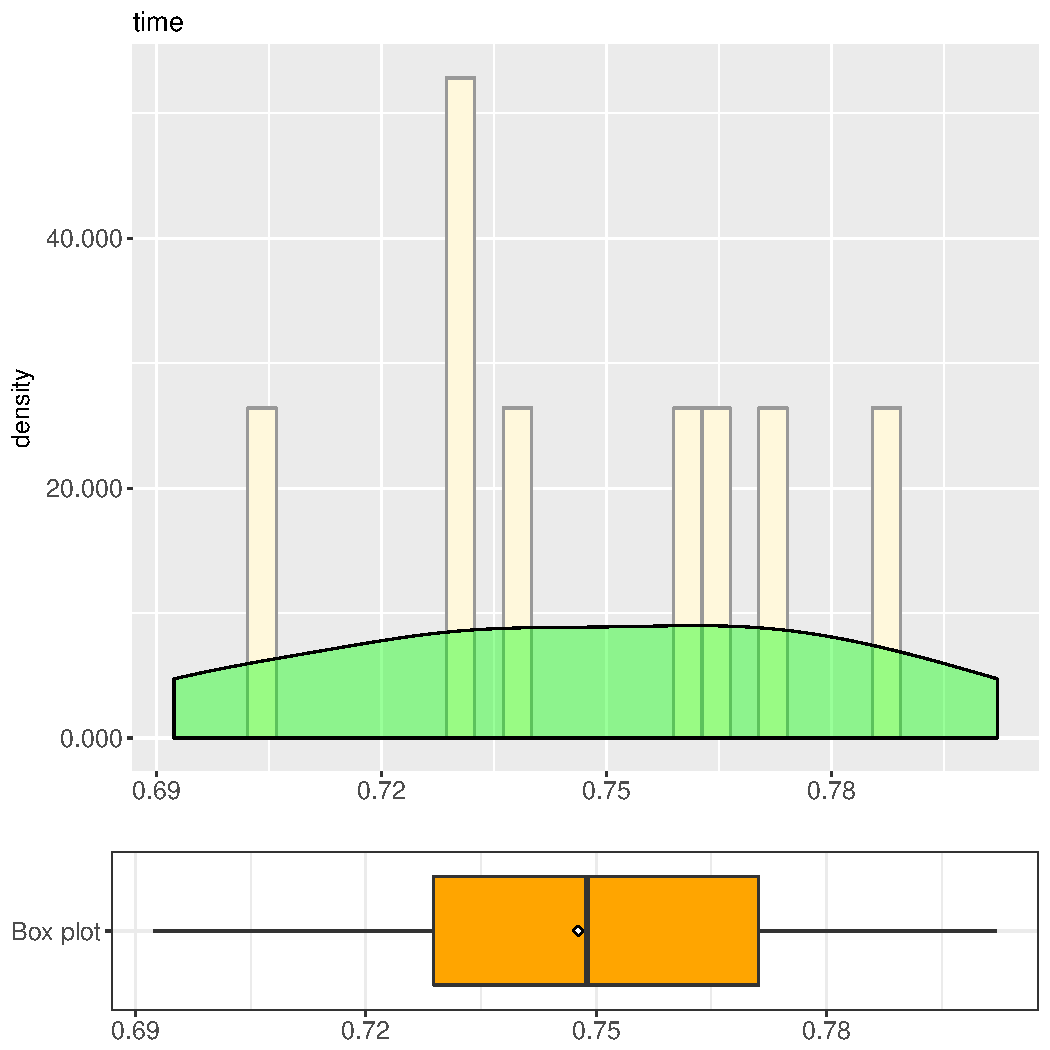
\includegraphics[width=\maxwidth]{figure/RH1_Warm_steps40-1} 
\begin{kframe}\begin{verbatim}
## 
## 	Shapiro-Wilk normality test
## 
## data:  subset(json_data, treatment == "Warm" & object == "steps40")$time
## W = 0.96969, p-value = 0.888
## 
## [1] "Shapiro test: Null Hypothesis (normality) not rejected. P-value: 0.887960927324343"
\end{verbatim}
\end{kframe}
\end{knitrout}
  
 \textbf{Comparison}
  
\begin{knitrout}
\definecolor{shadecolor}{rgb}{0.969, 0.969, 0.969}\color{fgcolor}
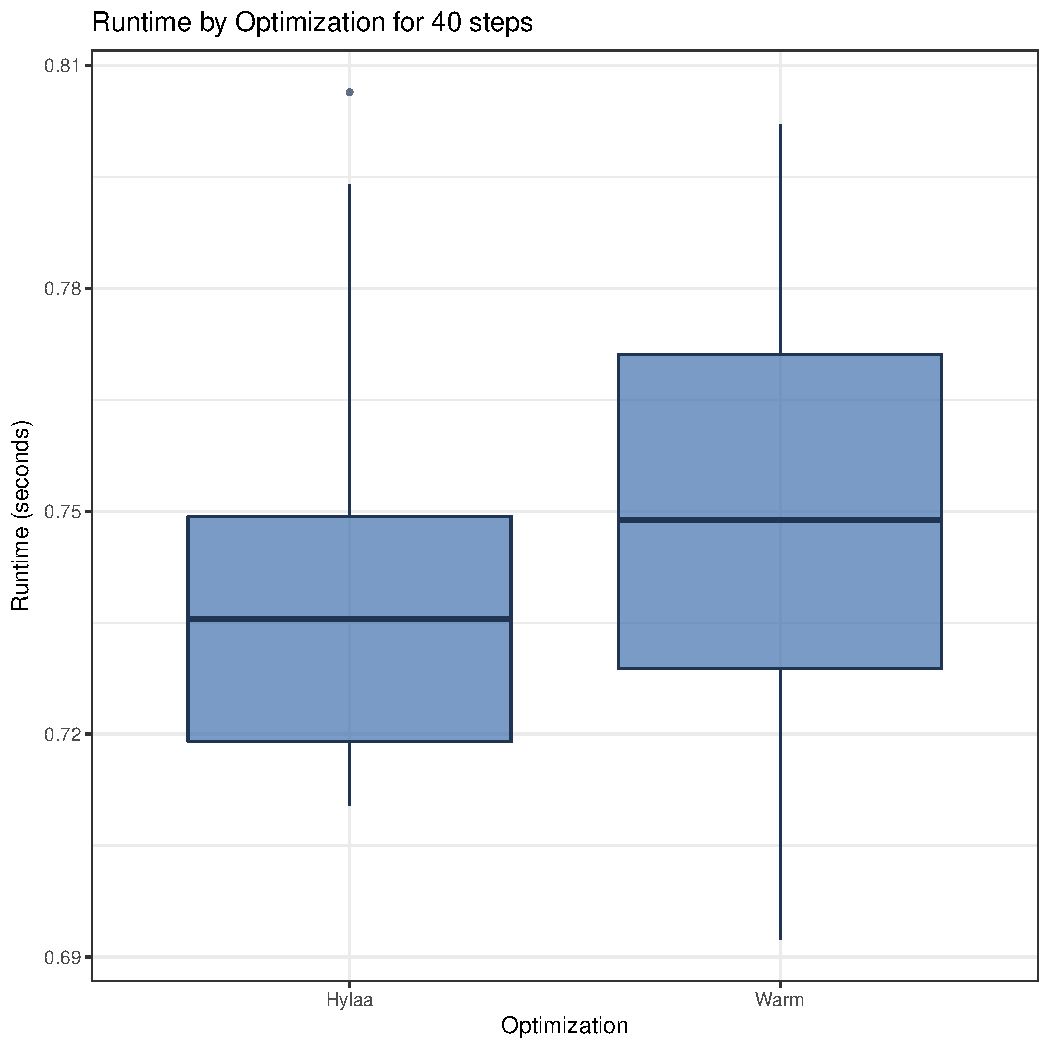
\includegraphics[width=\maxwidth]{figure/RH1_steps40-1} 
\begin{kframe}\begin{verbatim}
## [1] "Fisher's F-test to verify the homoskedasticity (homogeneity of variances)"
## 
## 	F test to compare two variances
## 
## data:  subset(json_data, treatment == "Hylaa" & object == "steps40")$time and subset(json_data, treatment == "Warm" & object == "steps40")$time
## F = 0.84799, num df = 9, denom df = 9, p-value = 0.81
## alternative hypothesis: true ratio of variances is not equal to 1
## 95 percent confidence interval:
##  0.2106286 3.4140009
## sample estimates:
## ratio of variances 
##          0.8479895 
## 
## [1] "Homogeneity of variances: TRUE. P-value: 0.80999212614282"
## [1] "Assuming that the two samples are taken from populations that follow a Gaussian distribution (if we cannot assume that, we must solve this problem using the non-parametric test called Wilcoxon-Mann-Whitney test)"
## 
## 	Two Sample t-test
## 
## data:  subset(json_data, treatment == "Hylaa" & object == "steps40")$time and subset(json_data, treatment == "Warm" & object == "steps40")$time
## t = -0.293, df = 18, p-value = 0.7729
## alternative hypothesis: true difference in means is not equal to 0
## 95 percent confidence interval:
##  -0.03658369  0.02762840
## sample estimates:
## mean of x mean of y 
## 0.7431680 0.7476457 
## 
## [1] "T-test: Null Hypothesis not rejected. P-value: 0.772870604957377"
## [1] ""
## [1] "Means comparison"
## [1] "Mean Runtime for Hylaa:  0.7431680440903"
## [1] "Mean Runtime for Warm:  0.7476456880569"
## [1] "Absolute difference:  0.0044776439666"
## Runtime for Warm is  0.60250760271602 % greater than 
## Runtime for Hylaa
\end{verbatim}
\end{kframe}
\end{knitrout}


\subsubsection{RH1.3: Object 53 steps}

 \textbf{Runtime for Hylaa}
\begin{knitrout}
\definecolor{shadecolor}{rgb}{0.969, 0.969, 0.969}\color{fgcolor}\begin{kframe}
\begin{verbatim}
## [1] "Sample size:  10"
##    Min. 1st Qu.  Median    Mean 3rd Qu.    Max. 
##  0.6997  0.7278  0.7623  0.7544  0.7732  0.8157
\end{verbatim}
\end{kframe}
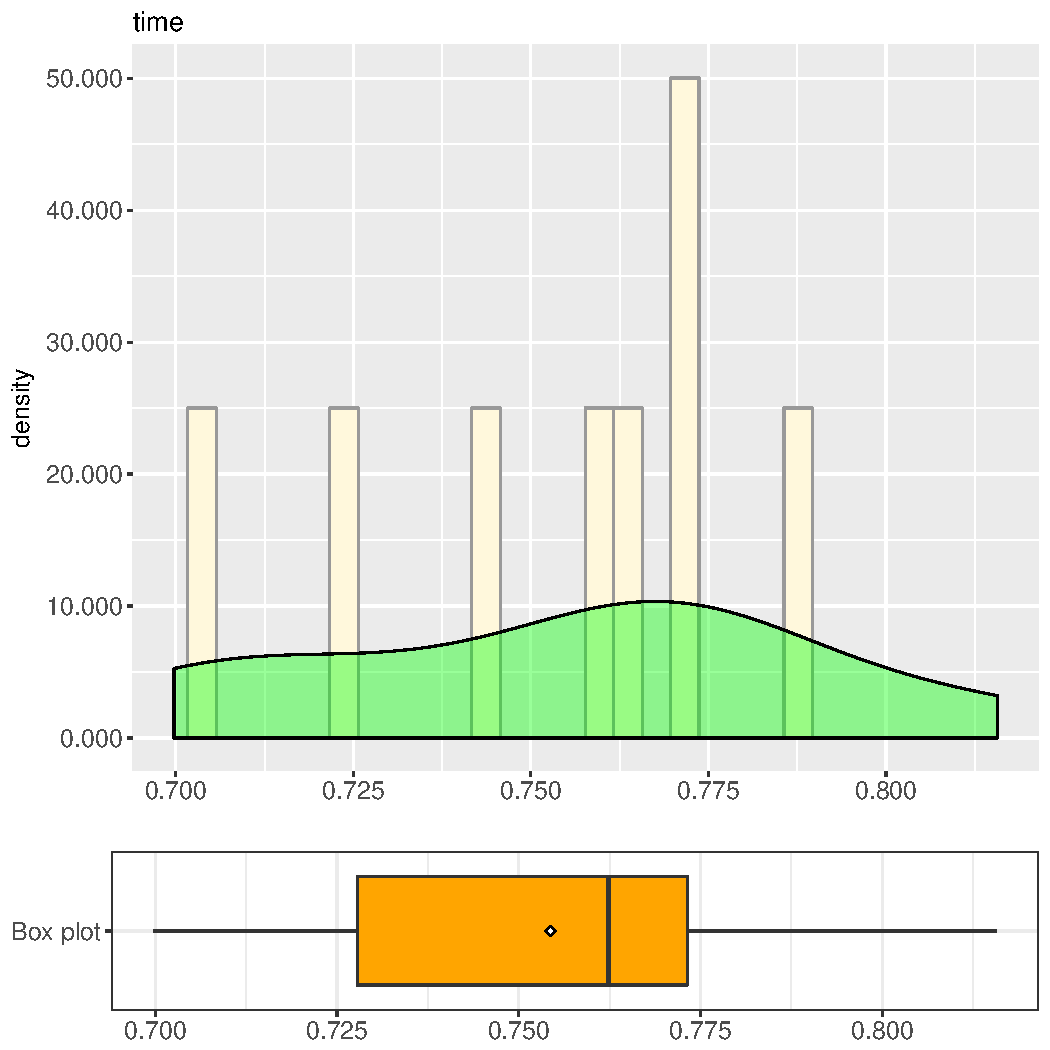
\includegraphics[width=\maxwidth]{figure/RH1_Hylaa_steps53-1} 
\begin{kframe}\begin{verbatim}
## 
## 	Shapiro-Wilk normality test
## 
## data:  subset(json_data, treatment == "Hylaa" & object == "steps53")$time
## W = 0.95914, p-value = 0.776
## 
## [1] "Shapiro test: Null Hypothesis (normality) not rejected. P-value: 0.776029544672673"
\end{verbatim}
\end{kframe}
\end{knitrout}
 \textbf{Runtime for Warm}
\begin{knitrout}
\definecolor{shadecolor}{rgb}{0.969, 0.969, 0.969}\color{fgcolor}\begin{kframe}
\begin{verbatim}
## [1] "Sample size:  10"
##    Min. 1st Qu.  Median    Mean 3rd Qu.    Max. 
##  0.7133  0.7471  0.7863  0.7712  0.7937  0.8130
\end{verbatim}
\end{kframe}
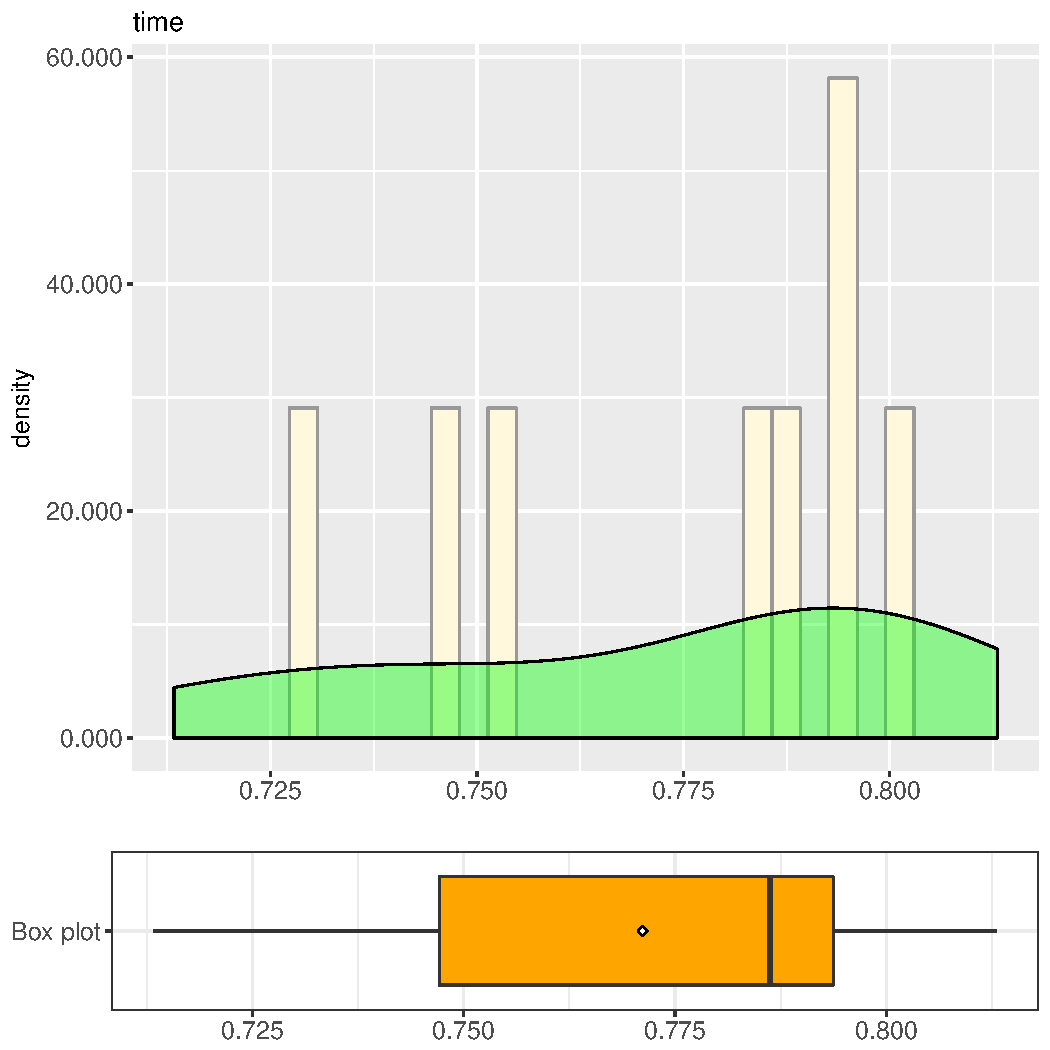
\includegraphics[width=\maxwidth]{figure/RH1_Warm_steps53-1} 
\begin{kframe}\begin{verbatim}
## 
## 	Shapiro-Wilk normality test
## 
## data:  subset(json_data, treatment == "Warm" & object == "steps53")$time
## W = 0.90652, p-value = 0.2579
## 
## [1] "Shapiro test: Null Hypothesis (normality) not rejected. P-value: 0.257924554875211"
\end{verbatim}
\end{kframe}
\end{knitrout}
  
 \textbf{Comparison}
  
\begin{knitrout}
\definecolor{shadecolor}{rgb}{0.969, 0.969, 0.969}\color{fgcolor}
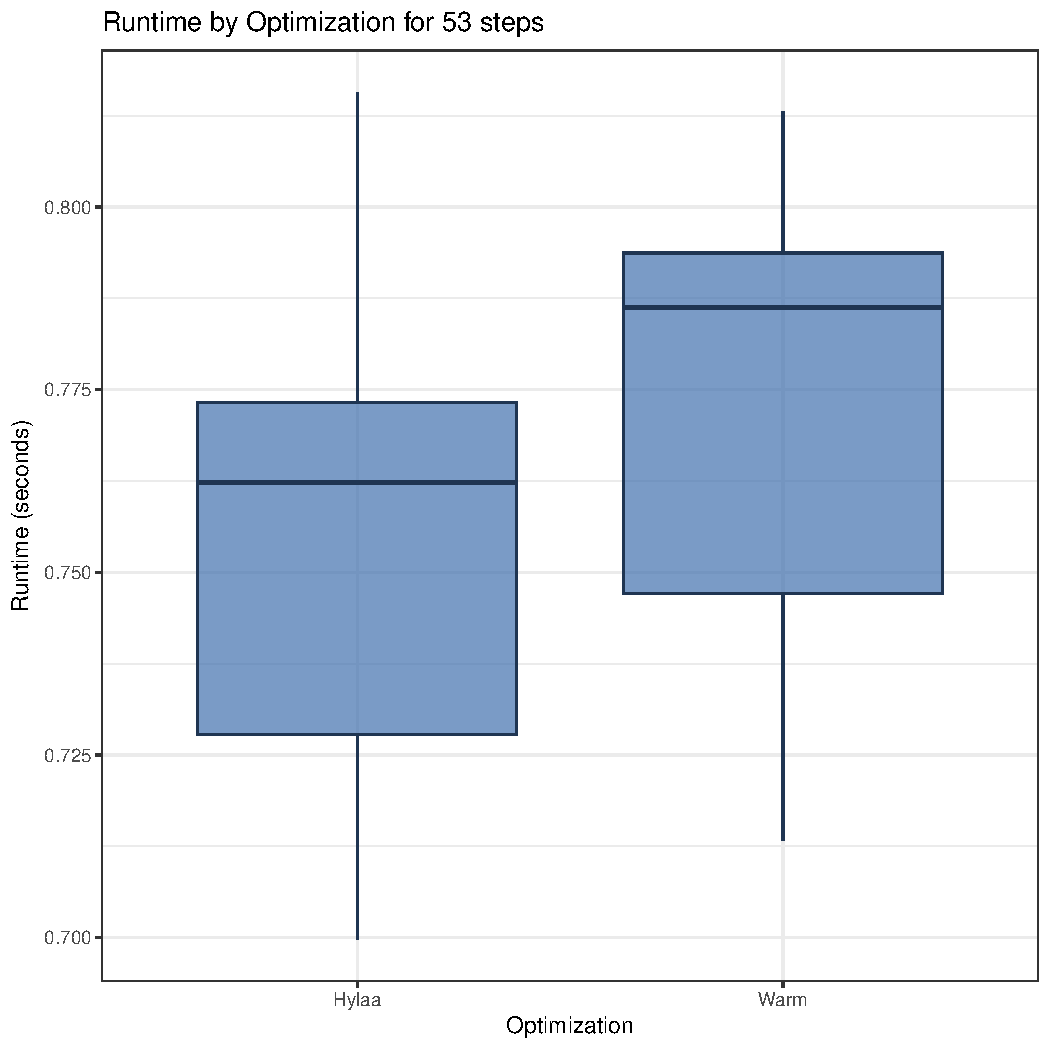
\includegraphics[width=\maxwidth]{figure/RH1_steps53-1} 
\begin{kframe}\begin{verbatim}
## [1] "Fisher's F-test to verify the homoskedasticity (homogeneity of variances)"
## 
## 	F test to compare two variances
## 
## data:  subset(json_data, treatment == "Hylaa" & object == "steps53")$time and subset(json_data, treatment == "Warm" & object == "steps53")$time
## F = 1.1697, num df = 9, denom df = 9, p-value = 0.8192
## alternative hypothesis: true ratio of variances is not equal to 1
## 95 percent confidence interval:
##  0.2905437 4.7093146
## sample estimates:
## ratio of variances 
##           1.169727 
## 
## [1] "Homogeneity of variances: TRUE. P-value: 0.819169805244097"
## [1] "Assuming that the two samples are taken from populations that follow a Gaussian distribution (if we cannot assume that, we must solve this problem using the non-parametric test called Wilcoxon-Mann-Whitney test)"
## 
## 	Two Sample t-test
## 
## data:  subset(json_data, treatment == "Hylaa" & object == "steps53")$time and subset(json_data, treatment == "Warm" & object == "steps53")$time
## t = -1.0624, df = 18, p-value = 0.3021
## alternative hypothesis: true difference in means is not equal to 0
## 95 percent confidence interval:
##  -0.05003068  0.01642558
## sample estimates:
## mean of x mean of y 
## 0.7543800 0.7711825 
## 
## [1] "T-test: Null Hypothesis not rejected. P-value: 0.302110336252165"
## [1] ""
## [1] "Means comparison"
## [1] "Mean Runtime for Hylaa:  0.7543799638747"
## [1] "Mean Runtime for Warm:  0.7711825132371"
## [1] "Absolute difference:  0.0168025493624"
## Runtime for Warm is  2.22733240104861 % greater than 
## Runtime for Hylaa
\end{verbatim}
\end{kframe}
\end{knitrout}


\subsubsection{RH1.4: Object 68 steps}

 \textbf{Runtime for Hylaa}
\begin{knitrout}
\definecolor{shadecolor}{rgb}{0.969, 0.969, 0.969}\color{fgcolor}\begin{kframe}
\begin{verbatim}
## [1] "Sample size:  10"
##    Min. 1st Qu.  Median    Mean 3rd Qu.    Max. 
##  0.7376  0.7525  0.7618  0.7645  0.7681  0.8046
\end{verbatim}
\end{kframe}
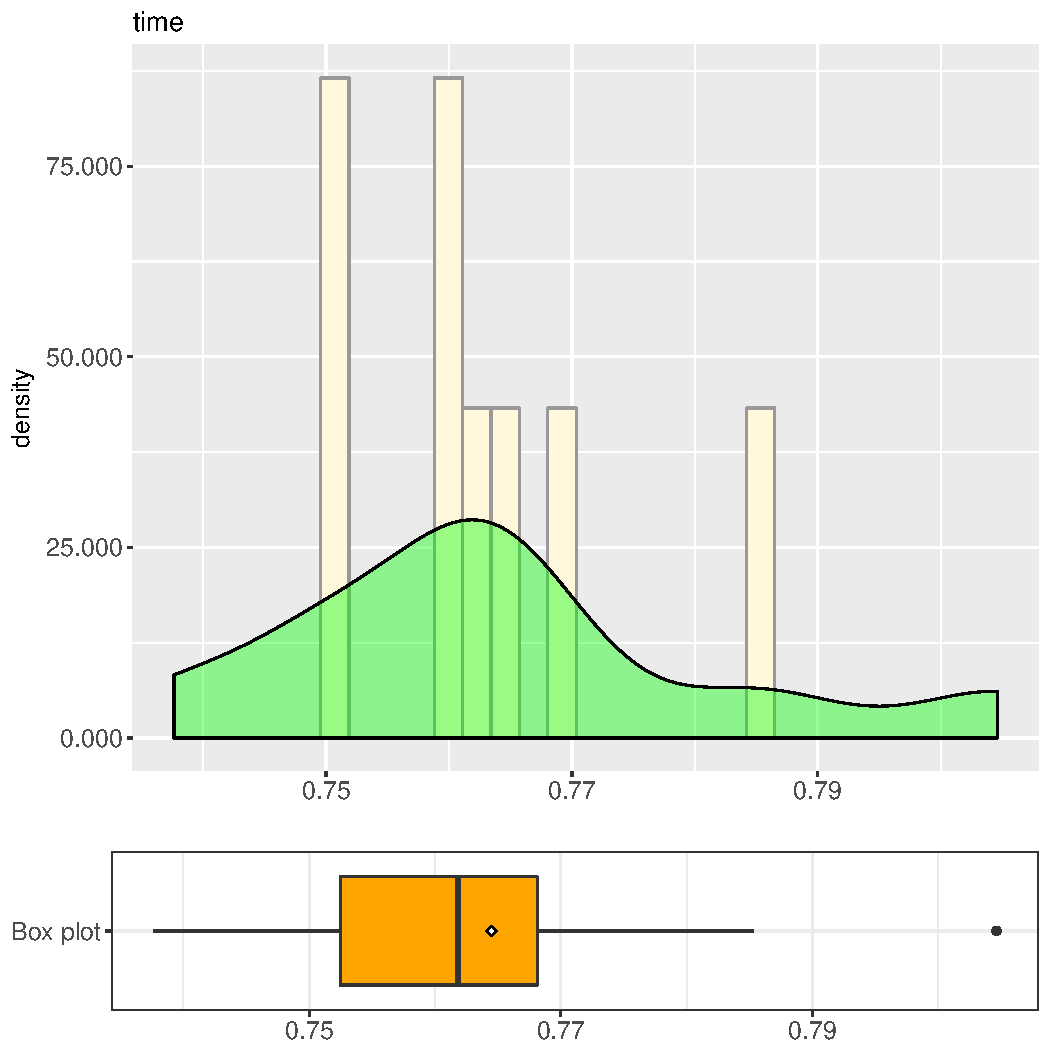
\includegraphics[width=\maxwidth]{figure/RH1_Hylaa_steps68-1} 
\begin{kframe}\begin{verbatim}
## 
## 	Shapiro-Wilk normality test
## 
## data:  subset(json_data, treatment == "Hylaa" & object == "steps68")$time
## W = 0.92932, p-value = 0.4412
## 
## [1] "Shapiro test: Null Hypothesis (normality) not rejected. P-value: 0.44123425938003"
\end{verbatim}
\end{kframe}
\end{knitrout}
 \textbf{Runtime for Warm}
\begin{knitrout}
\definecolor{shadecolor}{rgb}{0.969, 0.969, 0.969}\color{fgcolor}\begin{kframe}
\begin{verbatim}
## [1] "Sample size:  10"
##    Min. 1st Qu.  Median    Mean 3rd Qu.    Max. 
##  0.6689  0.7051  0.7280  0.7296  0.7625  0.7815
\end{verbatim}
\end{kframe}
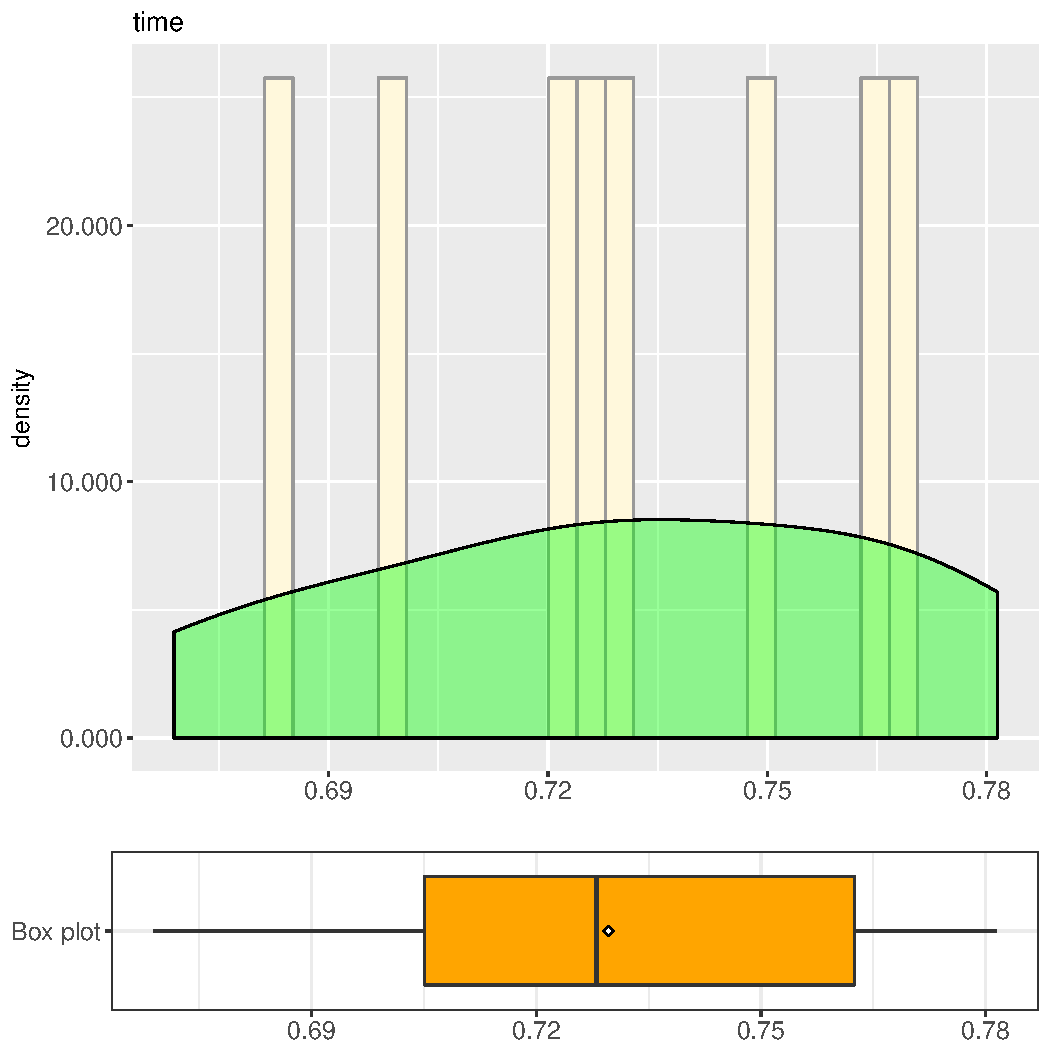
\includegraphics[width=\maxwidth]{figure/RH1_Warm_steps68-1} 
\begin{kframe}\begin{verbatim}
## 
## 	Shapiro-Wilk normality test
## 
## data:  subset(json_data, treatment == "Warm" & object == "steps68")$time
## W = 0.95718, p-value = 0.7533
## 
## [1] "Shapiro test: Null Hypothesis (normality) not rejected. P-value: 0.753294225891065"
\end{verbatim}
\end{kframe}
\end{knitrout}
  
 \textbf{Comparison}
  
\begin{knitrout}
\definecolor{shadecolor}{rgb}{0.969, 0.969, 0.969}\color{fgcolor}
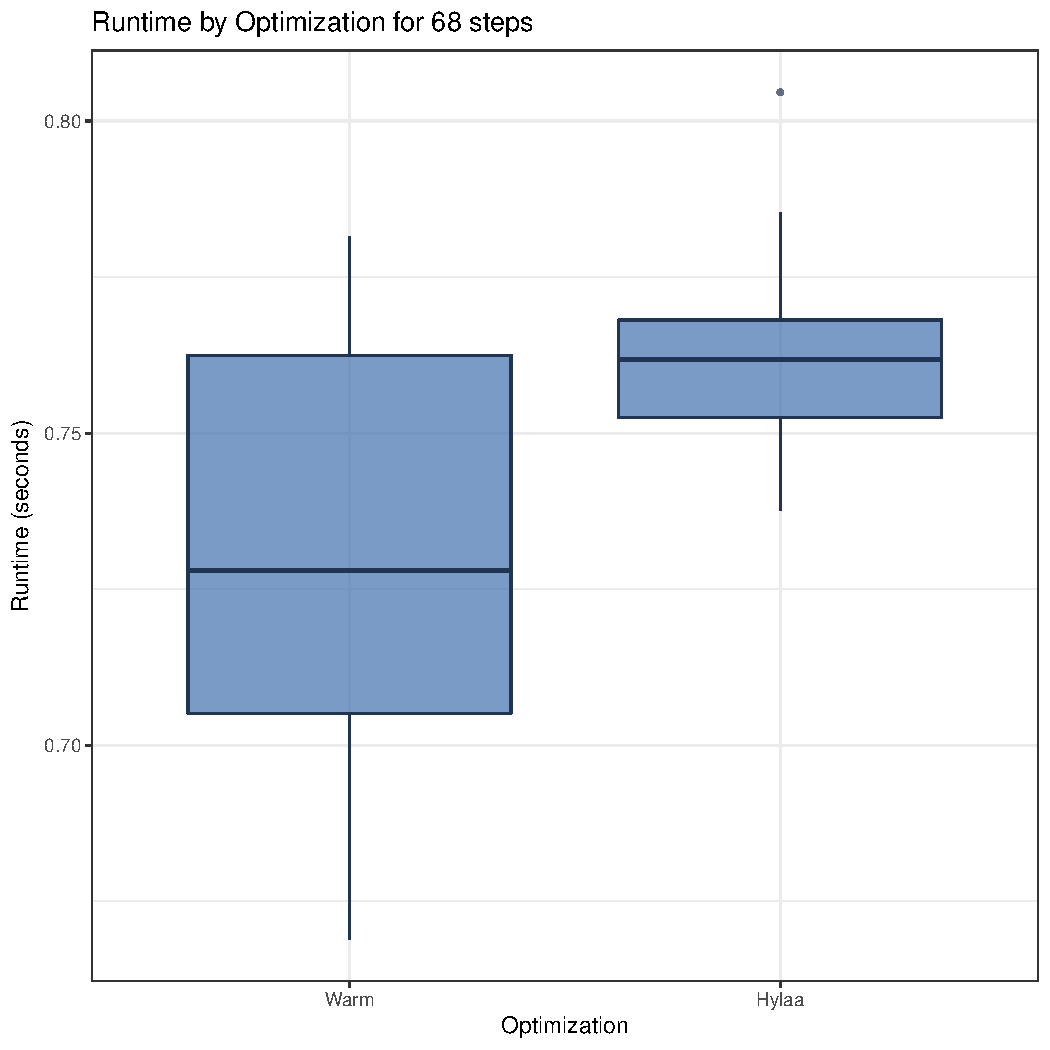
\includegraphics[width=\maxwidth]{figure/RH1_steps68-1} 
\begin{kframe}\begin{verbatim}
## [1] "Fisher's F-test to verify the homoskedasticity (homogeneity of variances)"
## 
## 	F test to compare two variances
## 
## data:  subset(json_data, treatment == "Hylaa" & object == "steps68")$time and subset(json_data, treatment == "Warm" & object == "steps68")$time
## F = 0.25801, num df = 9, denom df = 9, p-value = 0.05614
## alternative hypothesis: true ratio of variances is not equal to 1
## 95 percent confidence interval:
##  0.06408574 1.03874195
## sample estimates:
## ratio of variances 
##          0.2580088 
## 
## [1] "Homogeneity of variances: TRUE. P-value: 0.0561446074554752"
## [1] "Assuming that the two samples are taken from populations that follow a Gaussian distribution (if we cannot assume that, we must solve this problem using the non-parametric test called Wilcoxon-Mann-Whitney test)"
## 
## 	Two Sample t-test
## 
## data:  subset(json_data, treatment == "Hylaa" & object == "steps68")$time and subset(json_data, treatment == "Warm" & object == "steps68")$time
## t = 2.6236, df = 18, p-value = 0.01722
## alternative hypothesis: true difference in means is not equal to 0
## 95 percent confidence interval:
##  0.006940516 0.062738744
## sample estimates:
## mean of x mean of y 
## 0.7644785 0.7296388 
## 
## [1] "T-test: Null Hypothesis rejected. P-value: 0.0172232044414237"
## [1] ""
## [1] "Means comparison"
## [1] "Mean Runtime for Hylaa:  0.7644784688949"
## [1] "Mean Runtime for Warm:  0.7296388387681"
## [1] "Absolute difference:  0.0348396301268"
## Runtime for Hylaa is  4.77491442007421 % greater than 
##  Runtime for Warm
\end{verbatim}
\end{kframe}
\end{knitrout}


\subsubsection{RH1.5: Object 89 steps}

 \textbf{Runtime for Hylaa}
\begin{knitrout}
\definecolor{shadecolor}{rgb}{0.969, 0.969, 0.969}\color{fgcolor}\begin{kframe}
\begin{verbatim}
## [1] "Sample size:  10"
##    Min. 1st Qu.  Median    Mean 3rd Qu.    Max. 
##  0.7273  0.7541  0.7716  0.7796  0.8069  0.8377
\end{verbatim}
\end{kframe}
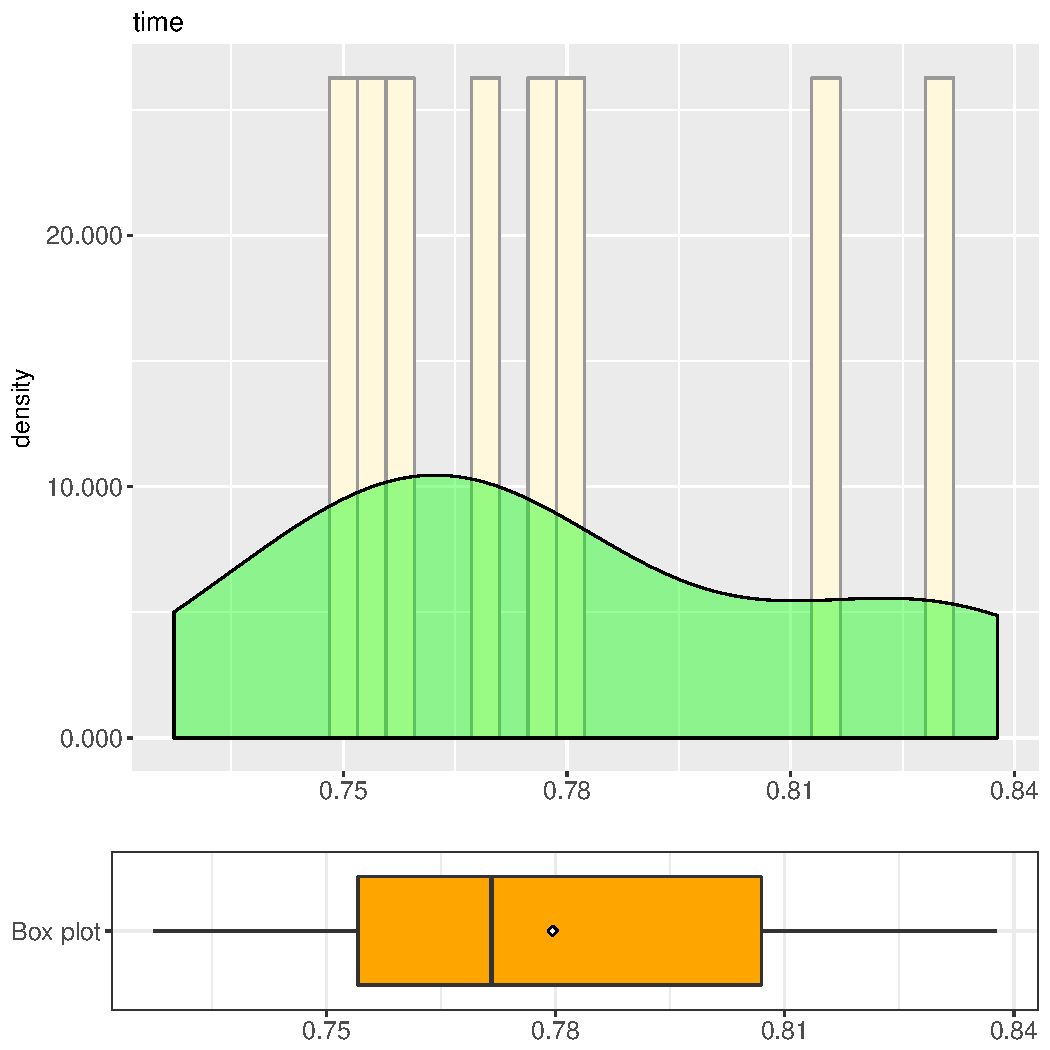
\includegraphics[width=\maxwidth]{figure/RH1_Hylaa_steps89-1} 
\begin{kframe}\begin{verbatim}
## 
## 	Shapiro-Wilk normality test
## 
## data:  subset(json_data, treatment == "Hylaa" & object == "steps89")$time
## W = 0.92836, p-value = 0.4319
## 
## [1] "Shapiro test: Null Hypothesis (normality) not rejected. P-value: 0.431928741976726"
\end{verbatim}
\end{kframe}
\end{knitrout}
 \textbf{Runtime for Warm}
\begin{knitrout}
\definecolor{shadecolor}{rgb}{0.969, 0.969, 0.969}\color{fgcolor}\begin{kframe}
\begin{verbatim}
## [1] "Sample size:  10"
##    Min. 1st Qu.  Median    Mean 3rd Qu.    Max. 
##  0.7299  0.7413  0.7570  0.7551  0.7618  0.7850
\end{verbatim}
\end{kframe}
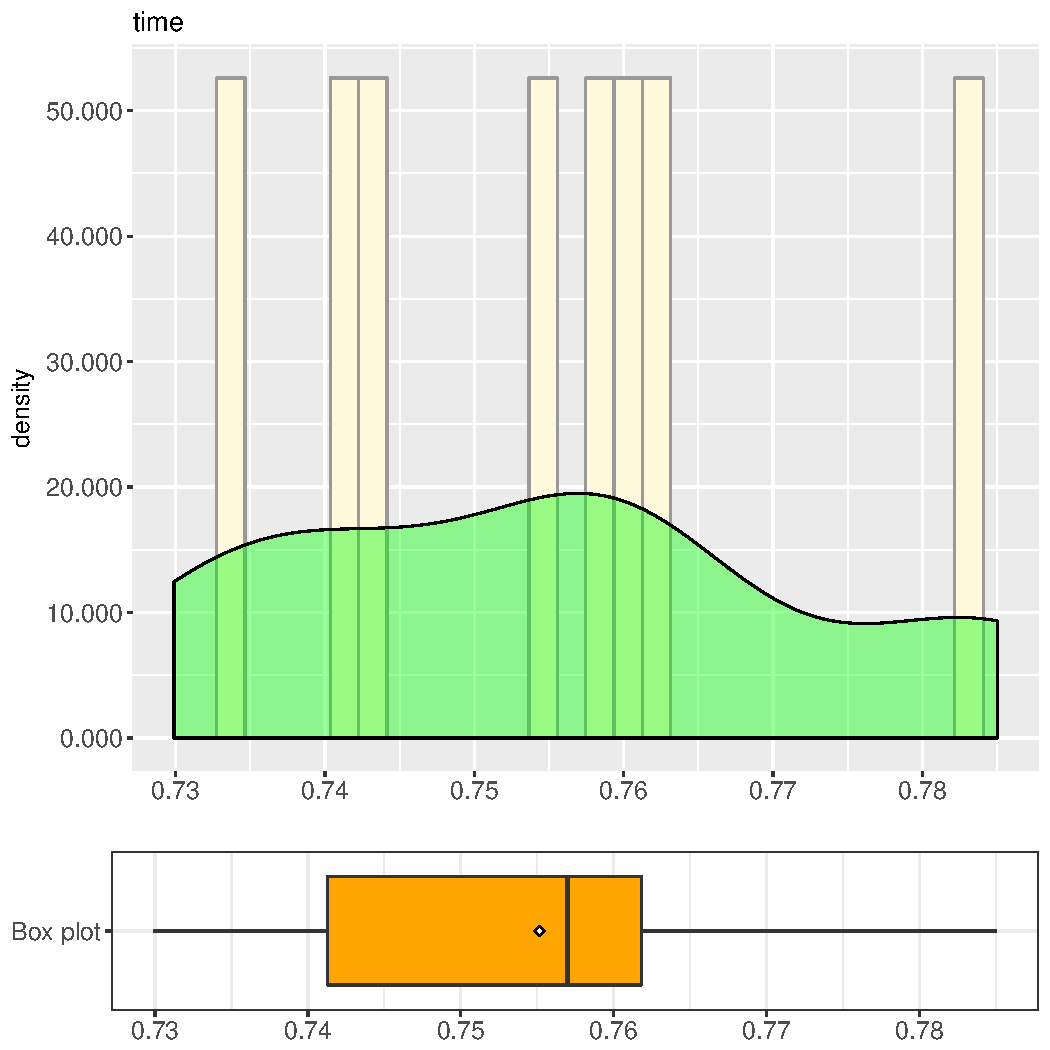
\includegraphics[width=\maxwidth]{figure/RH1_Warm_steps89-1} 
\begin{kframe}\begin{verbatim}
## 
## 	Shapiro-Wilk normality test
## 
## data:  subset(json_data, treatment == "Warm" & object == "steps89")$time
## W = 0.93381, p-value = 0.4864
## 
## [1] "Shapiro test: Null Hypothesis (normality) not rejected. P-value: 0.48644486648755"
\end{verbatim}
\end{kframe}
\end{knitrout}
  
 \textbf{Comparison}
  
\begin{knitrout}
\definecolor{shadecolor}{rgb}{0.969, 0.969, 0.969}\color{fgcolor}
\includegraphics[width=\maxwidth]{figure/RH1_steps89-1} 
\begin{kframe}\begin{verbatim}
## [1] "Fisher's F-test to verify the homoskedasticity (homogeneity of variances)"
## 
## 	F test to compare two variances
## 
## data:  subset(json_data, treatment == "Hylaa" & object == "steps89")$time and subset(json_data, treatment == "Warm" & object == "steps89")$time
## F = 3.7978, num df = 9, denom df = 9, p-value = 0.0597
## alternative hypothesis: true ratio of variances is not equal to 1
## 95 percent confidence interval:
##   0.9433294 15.2900768
## sample estimates:
## ratio of variances 
##           3.797839 
## 
## [1] "Homogeneity of variances: TRUE. P-value: 0.0596953035873224"
## [1] "Assuming that the two samples are taken from populations that follow a Gaussian distribution (if we cannot assume that, we must solve this problem using the non-parametric test called Wilcoxon-Mann-Whitney test)"
## 
## 	Two Sample t-test
## 
## data:  subset(json_data, treatment == "Hylaa" & object == "steps89")$time and subset(json_data, treatment == "Warm" & object == "steps89")$time
## t = 1.8721, df = 18, p-value = 0.07753
## alternative hypothesis: true difference in means is not equal to 0
## 95 percent confidence interval:
##  -0.002991089  0.051935323
## sample estimates:
## mean of x mean of y 
## 0.7796074 0.7551353 
## 
## [1] "T-test: Null Hypothesis not rejected. P-value: 0.0775319544685017"
## [1] ""
## [1] "Means comparison"
## [1] "Mean Runtime for Hylaa:  0.7796074151993"
## [1] "Mean Runtime for Warm:  0.7551352977755"
## [1] "Absolute difference:  0.0244721174238"
## Runtime for Hylaa is  3.24075930444394 % greater than 
##  Runtime for Warm
\end{verbatim}
\end{kframe}
\end{knitrout}


\subsubsection{RH1.6: Object 116 steps}

 \textbf{Runtime for Hylaa}
\begin{knitrout}
\definecolor{shadecolor}{rgb}{0.969, 0.969, 0.969}\color{fgcolor}\begin{kframe}
\begin{verbatim}
## [1] "Sample size:  10"
##    Min. 1st Qu.  Median    Mean 3rd Qu.    Max. 
##  0.7306  0.7757  0.7947  0.7856  0.8101  0.8193
\end{verbatim}
\end{kframe}
\includegraphics[width=\maxwidth]{figure/RH1_Hylaa_steps116-1} 
\begin{kframe}\begin{verbatim}
## 
## 	Shapiro-Wilk normality test
## 
## data:  subset(json_data, treatment == "Hylaa" & object == "steps116")$time
## W = 0.86307, p-value = 0.08294
## 
## [1] "Shapiro test: Null Hypothesis (normality) not rejected. P-value: 0.0829366496429817"
\end{verbatim}
\end{kframe}
\end{knitrout}
 \textbf{Runtime for Warm}
\begin{knitrout}
\definecolor{shadecolor}{rgb}{0.969, 0.969, 0.969}\color{fgcolor}\begin{kframe}
\begin{verbatim}
## [1] "Sample size:  10"
##    Min. 1st Qu.  Median    Mean 3rd Qu.    Max. 
##  0.7072  0.7494  0.7662  0.7585  0.7697  0.7853
\end{verbatim}
\end{kframe}
\includegraphics[width=\maxwidth]{figure/RH1_Warm_steps116-1} 
\begin{kframe}\begin{verbatim}
## 
## 	Shapiro-Wilk normality test
## 
## data:  subset(json_data, treatment == "Warm" & object == "steps116")$time
## W = 0.9028, p-value = 0.2351
## 
## [1] "Shapiro test: Null Hypothesis (normality) not rejected. P-value: 0.235105043492915"
\end{verbatim}
\end{kframe}
\end{knitrout}
  
 \textbf{Comparison}
  
\begin{knitrout}
\definecolor{shadecolor}{rgb}{0.969, 0.969, 0.969}\color{fgcolor}
\includegraphics[width=\maxwidth]{figure/RH1_steps116-1} 
\begin{kframe}\begin{verbatim}
## [1] "Fisher's F-test to verify the homoskedasticity (homogeneity of variances)"
## 
## 	F test to compare two variances
## 
## data:  subset(json_data, treatment == "Hylaa" & object == "steps116")$time and subset(json_data, treatment == "Warm" & object == "steps116")$time
## F = 1.921, num df = 9, denom df = 9, p-value = 0.3449
## alternative hypothesis: true ratio of variances is not equal to 1
## 95 percent confidence interval:
##  0.4771615 7.7341344
## sample estimates:
## ratio of variances 
##            1.92105 
## 
## [1] "Homogeneity of variances: TRUE. P-value: 0.34490839218464"
## [1] "Assuming that the two samples are taken from populations that follow a Gaussian distribution (if we cannot assume that, we must solve this problem using the non-parametric test called Wilcoxon-Mann-Whitney test)"
## 
## 	Two Sample t-test
## 
## data:  subset(json_data, treatment == "Hylaa" & object == "steps116")$time and subset(json_data, treatment == "Warm" & object == "steps116")$time
## t = 2.1608, df = 18, p-value = 0.04443
## alternative hypothesis: true difference in means is not equal to 0
## 95 percent confidence interval:
##  0.0007511088 0.0534294656
## sample estimates:
## mean of x mean of y 
## 0.7855974 0.7585071 
## 
## [1] "T-test: Null Hypothesis rejected. P-value: 0.0444344497096994"
## [1] ""
## [1] "Means comparison"
## [1] "Mean Runtime for Hylaa:  0.7855973720549"
## [1] "Mean Runtime for Warm:  0.7585070848467"
## [1] "Absolute difference:  0.0270902872081999"
## Runtime for Hylaa is  3.57152724732625 % greater than 
##  Runtime for Warm
\end{verbatim}
\end{kframe}
\end{knitrout}


\subsubsection{RH1.7: Object 151 steps}

 \textbf{Runtime for Hylaa}
\begin{knitrout}
\definecolor{shadecolor}{rgb}{0.969, 0.969, 0.969}\color{fgcolor}\begin{kframe}
\begin{verbatim}
## [1] "Sample size:  10"
##    Min. 1st Qu.  Median    Mean 3rd Qu.    Max. 
##  0.7351  0.7457  0.7654  0.7718  0.7998  0.8188
\end{verbatim}
\end{kframe}
\includegraphics[width=\maxwidth]{figure/RH1_Hylaa_steps151-1} 
\begin{kframe}\begin{verbatim}
## 
## 	Shapiro-Wilk normality test
## 
## data:  subset(json_data, treatment == "Hylaa" & object == "steps151")$time
## W = 0.8855, p-value = 0.1508
## 
## [1] "Shapiro test: Null Hypothesis (normality) not rejected. P-value: 0.15083040609515"
\end{verbatim}
\end{kframe}
\end{knitrout}
 \textbf{Runtime for Warm}
\begin{knitrout}
\definecolor{shadecolor}{rgb}{0.969, 0.969, 0.969}\color{fgcolor}\begin{kframe}
\begin{verbatim}
## [1] "Sample size:  10"
##    Min. 1st Qu.  Median    Mean 3rd Qu.    Max. 
##  0.6943  0.7228  0.7333  0.7388  0.7562  0.7936
\end{verbatim}
\end{kframe}
\includegraphics[width=\maxwidth]{figure/RH1_Warm_steps151-1} 
\begin{kframe}\begin{verbatim}
## 
## 	Shapiro-Wilk normality test
## 
## data:  subset(json_data, treatment == "Warm" & object == "steps151")$time
## W = 0.97251, p-value = 0.9131
## 
## [1] "Shapiro test: Null Hypothesis (normality) not rejected. P-value: 0.913118876153724"
\end{verbatim}
\end{kframe}
\end{knitrout}
  
 \textbf{Comparison}
  
\begin{knitrout}
\definecolor{shadecolor}{rgb}{0.969, 0.969, 0.969}\color{fgcolor}
\includegraphics[width=\maxwidth]{figure/RH1_steps151-1} 
\begin{kframe}\begin{verbatim}
## [1] "Fisher's F-test to verify the homoskedasticity (homogeneity of variances)"
## 
## 	F test to compare two variances
## 
## data:  subset(json_data, treatment == "Hylaa" & object == "steps151")$time and subset(json_data, treatment == "Warm" & object == "steps151")$time
## F = 1.3273, num df = 9, denom df = 9, p-value = 0.68
## alternative hypothesis: true ratio of variances is not equal to 1
## 95 percent confidence interval:
##  0.3296822 5.3436964
## sample estimates:
## ratio of variances 
##           1.327299 
## 
## [1] "Homogeneity of variances: TRUE. P-value: 0.680017210850041"
## [1] "Assuming that the two samples are taken from populations that follow a Gaussian distribution (if we cannot assume that, we must solve this problem using the non-parametric test called Wilcoxon-Mann-Whitney test)"
## 
## 	Two Sample t-test
## 
## data:  subset(json_data, treatment == "Hylaa" & object == "steps151")$time and subset(json_data, treatment == "Warm" & object == "steps151")$time
## t = 2.4293, df = 18, p-value = 0.02583
## alternative hypothesis: true difference in means is not equal to 0
## 95 percent confidence interval:
##  0.004463071 0.061578399
## sample estimates:
## mean of x mean of y 
## 0.7718092 0.7387885 
## 
## [1] "T-test: Null Hypothesis rejected. P-value: 0.0258252063294328"
## [1] ""
## [1] "Means comparison"
## [1] "Mean Runtime for Hylaa:  0.7718092203141"
## [1] "Mean Runtime for Warm:  0.7387884855271"
## [1] "Absolute difference:  0.0330207347870001"
## Runtime for Hylaa is  4.46957897069023 % greater than 
##  Runtime for Warm
\end{verbatim}
\end{kframe}
\end{knitrout}


\subsubsection{RH1.8: Object 197 steps}

 \textbf{Runtime for Hylaa}
\begin{knitrout}
\definecolor{shadecolor}{rgb}{0.969, 0.969, 0.969}\color{fgcolor}\begin{kframe}
\begin{verbatim}
## [1] "Sample size:  10"
##    Min. 1st Qu.  Median    Mean 3rd Qu.    Max. 
##  0.6995  0.7490  0.7739  0.7777  0.8150  0.8338
\end{verbatim}
\end{kframe}
\includegraphics[width=\maxwidth]{figure/RH1_Hylaa_steps197-1} 
\begin{kframe}\begin{verbatim}
## 
## 	Shapiro-Wilk normality test
## 
## data:  subset(json_data, treatment == "Hylaa" & object == "steps197")$time
## W = 0.94142, p-value = 0.569
## 
## [1] "Shapiro test: Null Hypothesis (normality) not rejected. P-value: 0.568954856828926"
\end{verbatim}
\end{kframe}
\end{knitrout}
 \textbf{Runtime for Warm}
\begin{knitrout}
\definecolor{shadecolor}{rgb}{0.969, 0.969, 0.969}\color{fgcolor}\begin{kframe}
\begin{verbatim}
## [1] "Sample size:  10"
##    Min. 1st Qu.  Median    Mean 3rd Qu.    Max. 
##  0.6681  0.7978  0.8192  0.7995  0.8279  0.8340
\end{verbatim}
\end{kframe}
\includegraphics[width=\maxwidth]{figure/RH1_Warm_steps197-1} 
\begin{kframe}\begin{verbatim}
## 
## 	Shapiro-Wilk normality test
## 
## data:  subset(json_data, treatment == "Warm" & object == "steps197")$time
## W = 0.68753, p-value = 0.0006223
## 
## [1] "Shapiro test: Null Hypothesis (normality) rejected. P-value: 0.000622303170797109"
\end{verbatim}
\end{kframe}
\end{knitrout}
  
 \textbf{Comparison}
  
\begin{knitrout}
\definecolor{shadecolor}{rgb}{0.969, 0.969, 0.969}\color{fgcolor}
\includegraphics[width=\maxwidth]{figure/RH1_steps197-1} 
\begin{kframe}\begin{verbatim}
## 
## 	Wilcoxon rank sum test
## 
## data:  time by treatment
## W = 27, p-value = 0.08921
## alternative hypothesis: true location shift is not equal to 0
## 
## [1] "Wilcoxon-Mann-Whitney test: Null Hypothesis not rejected. P-value: 0.0892095520578493"
## [1] ""
## [1] "Means comparison"
## [1] "Mean Runtime for Hylaa:  0.777667427063"
## [1] "Mean Runtime for Warm:  0.799469780922"
## [1] "Absolute difference:  0.021802353859"
## Runtime for Warm is  2.80355754918789 % greater than 
## Runtime for Hylaa
\end{verbatim}
\end{kframe}
\end{knitrout}


\subsubsection{RH1.9: Object 256 steps}

 \textbf{Runtime for Hylaa}
\begin{knitrout}
\definecolor{shadecolor}{rgb}{0.969, 0.969, 0.969}\color{fgcolor}\begin{kframe}
\begin{verbatim}
## [1] "Sample size:  10"
##    Min. 1st Qu.  Median    Mean 3rd Qu.    Max. 
##  0.7300  0.7691  0.7957  0.7970  0.8271  0.8542
\end{verbatim}
\end{kframe}
\includegraphics[width=\maxwidth]{figure/RH1_Hylaa_steps256-1} 
\begin{kframe}\begin{verbatim}
## 
## 	Shapiro-Wilk normality test
## 
## data:  subset(json_data, treatment == "Hylaa" & object == "steps256")$time
## W = 0.964, p-value = 0.8303
## 
## [1] "Shapiro test: Null Hypothesis (normality) not rejected. P-value: 0.830310406698625"
\end{verbatim}
\end{kframe}
\end{knitrout}
 \textbf{Runtime for Warm}
\begin{knitrout}
\definecolor{shadecolor}{rgb}{0.969, 0.969, 0.969}\color{fgcolor}\begin{kframe}
\begin{verbatim}
## [1] "Sample size:  10"
##    Min. 1st Qu.  Median    Mean 3rd Qu.    Max. 
##  0.7946  0.8232  0.8536  0.8482  0.8703  0.9003
\end{verbatim}
\end{kframe}
\includegraphics[width=\maxwidth]{figure/RH1_Warm_steps256-1} 
\begin{kframe}\begin{verbatim}
## 
## 	Shapiro-Wilk normality test
## 
## data:  subset(json_data, treatment == "Warm" & object == "steps256")$time
## W = 0.97206, p-value = 0.9092
## 
## [1] "Shapiro test: Null Hypothesis (normality) not rejected. P-value: 0.909224489734146"
\end{verbatim}
\end{kframe}
\end{knitrout}
  
 \textbf{Comparison}
  
\begin{knitrout}
\definecolor{shadecolor}{rgb}{0.969, 0.969, 0.969}\color{fgcolor}
\includegraphics[width=\maxwidth]{figure/RH1_steps256-1} 
\begin{kframe}\begin{verbatim}
## [1] "Fisher's F-test to verify the homoskedasticity (homogeneity of variances)"
## 
## 	F test to compare two variances
## 
## data:  subset(json_data, treatment == "Hylaa" & object == "steps256")$time and subset(json_data, treatment == "Warm" & object == "steps256")$time
## F = 1.4142, num df = 9, denom df = 9, p-value = 0.614
## alternative hypothesis: true ratio of variances is not equal to 1
## 95 percent confidence interval:
##  0.3512696 5.6935994
## sample estimates:
## ratio of variances 
##            1.41421 
## 
## [1] "Homogeneity of variances: TRUE. P-value: 0.613964351705911"
## [1] "Assuming that the two samples are taken from populations that follow a Gaussian distribution (if we cannot assume that, we must solve this problem using the non-parametric test called Wilcoxon-Mann-Whitney test)"
## 
## 	Two Sample t-test
## 
## data:  subset(json_data, treatment == "Hylaa" & object == "steps256")$time and subset(json_data, treatment == "Warm" & object == "steps256")$time
## t = -3.1826, df = 18, p-value = 0.005156
## alternative hypothesis: true difference in means is not equal to 0
## 95 percent confidence interval:
##  -0.08489653 -0.01738104
## sample estimates:
## mean of x mean of y 
## 0.7970330 0.8481718 
## 
## [1] "T-test: Null Hypothesis rejected. P-value: 0.00515550553759939"
## [1] ""
## [1] "Means comparison"
## [1] "Mean Runtime for Hylaa:  0.7970329999924"
## [1] "Mean Runtime for Warm:  0.8481717824937"
## [1] "Absolute difference:  0.0511387825013001"
## Runtime for Warm is  6.4161436856175 % greater than 
## Runtime for Hylaa
\end{verbatim}
\end{kframe}
\end{knitrout}


\subsubsection{RH1.10: Object 332 steps}

 \textbf{Runtime for Hylaa}
\begin{knitrout}
\definecolor{shadecolor}{rgb}{0.969, 0.969, 0.969}\color{fgcolor}\begin{kframe}
\begin{verbatim}
## [1] "Sample size:  10"
##    Min. 1st Qu.  Median    Mean 3rd Qu.    Max. 
##  0.7116  0.7462  0.7788  0.7682  0.7952  0.8058
\end{verbatim}
\end{kframe}
\includegraphics[width=\maxwidth]{figure/RH1_Hylaa_steps332-1} 
\begin{kframe}\begin{verbatim}
## 
## 	Shapiro-Wilk normality test
## 
## data:  subset(json_data, treatment == "Hylaa" & object == "steps332")$time
## W = 0.87995, p-value = 0.1303
## 
## [1] "Shapiro test: Null Hypothesis (normality) not rejected. P-value: 0.130315495202675"
\end{verbatim}
\end{kframe}
\end{knitrout}
 \textbf{Runtime for Warm}
\begin{knitrout}
\definecolor{shadecolor}{rgb}{0.969, 0.969, 0.969}\color{fgcolor}\begin{kframe}
\begin{verbatim}
## [1] "Sample size:  10"
##    Min. 1st Qu.  Median    Mean 3rd Qu.    Max. 
##  0.7992  0.8122  0.8202  0.8199  0.8297  0.8375
\end{verbatim}
\end{kframe}
\includegraphics[width=\maxwidth]{figure/RH1_Warm_steps332-1} 
\begin{kframe}\begin{verbatim}
## 
## 	Shapiro-Wilk normality test
## 
## data:  subset(json_data, treatment == "Warm" & object == "steps332")$time
## W = 0.96673, p-value = 0.859
## 
## [1] "Shapiro test: Null Hypothesis (normality) not rejected. P-value: 0.858987863455774"
\end{verbatim}
\end{kframe}
\end{knitrout}
  
 \textbf{Comparison}
  
\begin{knitrout}
\definecolor{shadecolor}{rgb}{0.969, 0.969, 0.969}\color{fgcolor}
\includegraphics[width=\maxwidth]{figure/RH1_steps332-1} 
\begin{kframe}\begin{verbatim}
## [1] "Fisher's F-test to verify the homoskedasticity (homogeneity of variances)"
## 
## 	F test to compare two variances
## 
## data:  subset(json_data, treatment == "Hylaa" & object == "steps332")$time and subset(json_data, treatment == "Warm" & object == "steps332")$time
## F = 8.1607, num df = 9, denom df = 9, p-value = 0.004485
## alternative hypothesis: true ratio of variances is not equal to 1
## 95 percent confidence interval:
##   2.027007 32.855000
## sample estimates:
## ratio of variances 
##           8.160717 
## 
## [1] "Homogeneity of variances: FALSE. P-value: 0.00448525981497427"
## [1] "Assuming that the two samples are taken from populations that follow a Gaussian distribution (if we cannot assume that, we must solve this problem using the non-parametric test called Wilcoxon-Mann-Whitney test)"
## 
## 	Welch Two Sample t-test
## 
## data:  subset(json_data, treatment == "Hylaa" & object == "steps332")$time and subset(json_data, treatment == "Warm" & object == "steps332")$time
## t = -4.4321, df = 11.173, p-value = 0.0009709
## alternative hypothesis: true difference in means is not equal to 0
## 95 percent confidence interval:
##  -0.07727876 -0.02605801
## sample estimates:
## mean of x mean of y 
## 0.7681974 0.8198658 
## 
## [1] "T-test: Null Hypothesis rejected. P-value: 0.000970941286228814"
## [1] ""
## [1] "Means comparison"
## [1] "Mean Runtime for Hylaa:  0.7681974172593"
## [1] "Mean Runtime for Warm:  0.8198657989502"
## [1] "Absolute difference:  0.0516683816908999"
## Runtime for Warm is  6.72592494195533 % greater than 
## Runtime for Hylaa
\end{verbatim}
\end{kframe}
\end{knitrout}


\subsubsection{RH1.11: Object 432 steps}

 \textbf{Runtime for Hylaa}
\begin{knitrout}
\definecolor{shadecolor}{rgb}{0.969, 0.969, 0.969}\color{fgcolor}\begin{kframe}
\begin{verbatim}
## [1] "Sample size:  10"
##    Min. 1st Qu.  Median    Mean 3rd Qu.    Max. 
##  0.7247  0.8047  0.8112  0.8107  0.8280  0.8544
\end{verbatim}
\end{kframe}
\includegraphics[width=\maxwidth]{figure/RH1_Hylaa_steps432-1} 
\begin{kframe}\begin{verbatim}
## 
## 	Shapiro-Wilk normality test
## 
## data:  subset(json_data, treatment == "Hylaa" & object == "steps432")$time
## W = 0.82468, p-value = 0.02887
## 
## [1] "Shapiro test: Null Hypothesis (normality) rejected. P-value: 0.0288658654097958"
\end{verbatim}
\end{kframe}
\end{knitrout}
 \textbf{Runtime for Warm}
\begin{knitrout}
\definecolor{shadecolor}{rgb}{0.969, 0.969, 0.969}\color{fgcolor}\begin{kframe}
\begin{verbatim}
## [1] "Sample size:  10"
##    Min. 1st Qu.  Median    Mean 3rd Qu.    Max. 
##  0.8355  0.8482  0.8939  0.8827  0.9070  0.9255
\end{verbatim}
\end{kframe}
\includegraphics[width=\maxwidth]{figure/RH1_Warm_steps432-1} 
\begin{kframe}\begin{verbatim}
## 
## 	Shapiro-Wilk normality test
## 
## data:  subset(json_data, treatment == "Warm" & object == "steps432")$time
## W = 0.886, p-value = 0.1528
## 
## [1] "Shapiro test: Null Hypothesis (normality) not rejected. P-value: 0.152792850523887"
\end{verbatim}
\end{kframe}
\end{knitrout}
  
 \textbf{Comparison}
  
\begin{knitrout}
\definecolor{shadecolor}{rgb}{0.969, 0.969, 0.969}\color{fgcolor}
\includegraphics[width=\maxwidth]{figure/RH1_steps432-1} 
\begin{kframe}\begin{verbatim}
## 
## 	Wilcoxon rank sum test
## 
## data:  time by treatment
## W = 4, p-value = 0.0001299
## alternative hypothesis: true location shift is not equal to 0
## 
## [1] "Wilcoxon-Mann-Whitney test: Null Hypothesis rejected. P-value: 0.000129901058693628"
## [1] ""
## [1] "Means comparison"
## [1] "Mean Runtime for Hylaa:  0.8107497930526"
## [1] "Mean Runtime for Warm:  0.8827400207519"
## [1] "Absolute difference:  0.0719902276993001"
## Runtime for Warm is  8.87946297565438 % greater than 
## Runtime for Hylaa
\end{verbatim}
\end{kframe}
\end{knitrout}


\subsubsection{RH1.12: Object 562 steps}

 \textbf{Runtime for Hylaa}
\begin{knitrout}
\definecolor{shadecolor}{rgb}{0.969, 0.969, 0.969}\color{fgcolor}\begin{kframe}
\begin{verbatim}
## [1] "Sample size:  10"
##    Min. 1st Qu.  Median    Mean 3rd Qu.    Max. 
##  0.7673  0.8121  0.8273  0.8211  0.8393  0.8746
\end{verbatim}
\end{kframe}
\includegraphics[width=\maxwidth]{figure/RH1_Hylaa_steps562-1} 
\begin{kframe}\begin{verbatim}
## 
## 	Shapiro-Wilk normality test
## 
## data:  subset(json_data, treatment == "Hylaa" & object == "steps562")$time
## W = 0.93601, p-value = 0.5095
## 
## [1] "Shapiro test: Null Hypothesis (normality) not rejected. P-value: 0.509497615860695"
\end{verbatim}
\end{kframe}
\end{knitrout}
 \textbf{Runtime for Warm}
\begin{knitrout}
\definecolor{shadecolor}{rgb}{0.969, 0.969, 0.969}\color{fgcolor}\begin{kframe}
\begin{verbatim}
## [1] "Sample size:  10"
##    Min. 1st Qu.  Median    Mean 3rd Qu.    Max. 
##  0.8617  0.9117  0.9595  0.9538  0.9929  1.0640
\end{verbatim}
\end{kframe}
\includegraphics[width=\maxwidth]{figure/RH1_Warm_steps562-1} 
\begin{kframe}\begin{verbatim}
## 
## 	Shapiro-Wilk normality test
## 
## data:  subset(json_data, treatment == "Warm" & object == "steps562")$time
## W = 0.98206, p-value = 0.9752
## 
## [1] "Shapiro test: Null Hypothesis (normality) not rejected. P-value: 0.97524131457127"
\end{verbatim}
\end{kframe}
\end{knitrout}
  
 \textbf{Comparison}
  
\begin{knitrout}
\definecolor{shadecolor}{rgb}{0.969, 0.969, 0.969}\color{fgcolor}
\includegraphics[width=\maxwidth]{figure/RH1_steps562-1} 
\begin{kframe}\begin{verbatim}
## [1] "Fisher's F-test to verify the homoskedasticity (homogeneity of variances)"
## 
## 	F test to compare two variances
## 
## data:  subset(json_data, treatment == "Hylaa" & object == "steps562")$time and subset(json_data, treatment == "Warm" & object == "steps562")$time
## F = 0.28648, num df = 9, denom df = 9, p-value = 0.0766
## alternative hypothesis: true ratio of variances is not equal to 1
## 95 percent confidence interval:
##  0.07115856 1.15338276
## sample estimates:
## ratio of variances 
##           0.286484 
## 
## [1] "Homogeneity of variances: TRUE. P-value: 0.0766012347568488"
## [1] "Assuming that the two samples are taken from populations that follow a Gaussian distribution (if we cannot assume that, we must solve this problem using the non-parametric test called Wilcoxon-Mann-Whitney test)"
## 
## 	Two Sample t-test
## 
## data:  subset(json_data, treatment == "Hylaa" & object == "steps562")$time and subset(json_data, treatment == "Warm" & object == "steps562")$time
## t = -6.09, df = 18, p-value = 9.377e-06
## alternative hypothesis: true difference in means is not equal to 0
## 95 percent confidence interval:
##  -0.17854537 -0.08695398
## sample estimates:
## mean of x mean of y 
## 0.8210984 0.9538481 
## 
## [1] "T-test: Null Hypothesis rejected. P-value: 9.37740126068088e-06"
## [1] ""
## [1] "Means comparison"
## [1] "Mean Runtime for Hylaa:  0.8210983753205"
## [1] "Mean Runtime for Warm:  0.9538480520249"
## [1] "Absolute difference:  0.1327496767044"
## Runtime for Warm is  16.1673291160251 % greater than 
## Runtime for Hylaa
\end{verbatim}
\end{kframe}
\end{knitrout}


\subsubsection{RH1.13: Object 731 steps}

 \textbf{Runtime for Hylaa}
\begin{knitrout}
\definecolor{shadecolor}{rgb}{0.969, 0.969, 0.969}\color{fgcolor}\begin{kframe}
\begin{verbatim}
## [1] "Sample size:  10"
##    Min. 1st Qu.  Median    Mean 3rd Qu.    Max. 
##  0.8045  0.8548  0.8749  0.8668  0.8896  0.8956
\end{verbatim}
\end{kframe}
\includegraphics[width=\maxwidth]{figure/RH1_Hylaa_steps731-1} 
\begin{kframe}\begin{verbatim}
## 
## 	Shapiro-Wilk normality test
## 
## data:  subset(json_data, treatment == "Hylaa" & object == "steps731")$time
## W = 0.86638, p-value = 0.09069
## 
## [1] "Shapiro test: Null Hypothesis (normality) not rejected. P-value: 0.0906925091728528"
\end{verbatim}
\end{kframe}
\end{knitrout}
 \textbf{Runtime for Warm}
\begin{knitrout}
\definecolor{shadecolor}{rgb}{0.969, 0.969, 0.969}\color{fgcolor}\begin{kframe}
\begin{verbatim}
## [1] "Sample size:  10"
##    Min. 1st Qu.  Median    Mean 3rd Qu.    Max. 
##   1.032   1.082   1.091   1.088   1.103   1.114
\end{verbatim}
\end{kframe}
\includegraphics[width=\maxwidth]{figure/RH1_Warm_steps731-1} 
\begin{kframe}\begin{verbatim}
## 
## 	Shapiro-Wilk normality test
## 
## data:  subset(json_data, treatment == "Warm" & object == "steps731")$time
## W = 0.83997, p-value = 0.04409
## 
## [1] "Shapiro test: Null Hypothesis (normality) rejected. P-value: 0.0440854589795451"
\end{verbatim}
\end{kframe}
\end{knitrout}
  
 \textbf{Comparison}
  
\begin{knitrout}
\definecolor{shadecolor}{rgb}{0.969, 0.969, 0.969}\color{fgcolor}
\includegraphics[width=\maxwidth]{figure/RH1_steps731-1} 
\begin{kframe}\begin{verbatim}
## 
## 	Wilcoxon rank sum test
## 
## data:  time by treatment
## W = 0, p-value = 1.083e-05
## alternative hypothesis: true location shift is not equal to 0
## 
## [1] "Wilcoxon-Mann-Whitney test: Null Hypothesis rejected. P-value: 1.0825088224469e-05"
## [1] ""
## [1] "Means comparison"
## [1] "Mean Runtime for Hylaa:  0.8668062448501"
## [1] "Mean Runtime for Warm:  1.088253617287"
## [1] "Absolute difference:  0.2214473724369"
## Runtime for Warm is  25.5475054261054 % greater than 
## Runtime for Hylaa
\end{verbatim}
\end{kframe}
\end{knitrout}


\subsubsection{RH1.14: Object 951 steps}

 \textbf{Runtime for Hylaa}
\begin{knitrout}
\definecolor{shadecolor}{rgb}{0.969, 0.969, 0.969}\color{fgcolor}\begin{kframe}
\begin{verbatim}
## [1] "Sample size:  10"
##    Min. 1st Qu.  Median    Mean 3rd Qu.    Max. 
##  0.8356  0.8536  0.8991  0.8888  0.9216  0.9388
\end{verbatim}
\end{kframe}
\includegraphics[width=\maxwidth]{figure/RH1_Hylaa_steps951-1} 
\begin{kframe}\begin{verbatim}
## 
## 	Shapiro-Wilk normality test
## 
## data:  subset(json_data, treatment == "Hylaa" & object == "steps951")$time
## W = 0.90483, p-value = 0.2474
## 
## [1] "Shapiro test: Null Hypothesis (normality) not rejected. P-value: 0.247358608075924"
\end{verbatim}
\end{kframe}
\end{knitrout}
 \textbf{Runtime for Warm}
\begin{knitrout}
\definecolor{shadecolor}{rgb}{0.969, 0.969, 0.969}\color{fgcolor}\begin{kframe}
\begin{verbatim}
## [1] "Sample size:  10"
##    Min. 1st Qu.  Median    Mean 3rd Qu.    Max. 
##   1.230   1.294   1.306   1.302   1.313   1.338
\end{verbatim}
\end{kframe}
\includegraphics[width=\maxwidth]{figure/RH1_Warm_steps951-1} 
\begin{kframe}\begin{verbatim}
## 
## 	Shapiro-Wilk normality test
## 
## data:  subset(json_data, treatment == "Warm" & object == "steps951")$time
## W = 0.84474, p-value = 0.05027
## 
## [1] "Shapiro test: Null Hypothesis (normality) not rejected. P-value: 0.0502723510901298"
\end{verbatim}
\end{kframe}
\end{knitrout}
  
 \textbf{Comparison}
  
\begin{knitrout}
\definecolor{shadecolor}{rgb}{0.969, 0.969, 0.969}\color{fgcolor}
\includegraphics[width=\maxwidth]{figure/RH1_steps951-1} 
\begin{kframe}\begin{verbatim}
## [1] "Fisher's F-test to verify the homoskedasticity (homogeneity of variances)"
## 
## 	F test to compare two variances
## 
## data:  subset(json_data, treatment == "Hylaa" & object == "steps951")$time and subset(json_data, treatment == "Warm" & object == "steps951")$time
## F = 1.7784, num df = 9, denom df = 9, p-value = 0.404
## alternative hypothesis: true ratio of variances is not equal to 1
## 95 percent confidence interval:
##  0.4417271 7.1597900
## sample estimates:
## ratio of variances 
##           1.778391 
## 
## [1] "Homogeneity of variances: TRUE. P-value: 0.404041921624122"
## [1] "Assuming that the two samples are taken from populations that follow a Gaussian distribution (if we cannot assume that, we must solve this problem using the non-parametric test called Wilcoxon-Mann-Whitney test)"
## 
## 	Two Sample t-test
## 
## data:  subset(json_data, treatment == "Hylaa" & object == "steps951")$time and subset(json_data, treatment == "Warm" & object == "steps951")$time
## t = -26.866, df = 18, p-value = 5.606e-16
## alternative hypothesis: true difference in means is not equal to 0
## 95 percent confidence interval:
##  -0.4451837 -0.3806062
## sample estimates:
## mean of x mean of y 
## 0.8888239 1.3017189 
## 
## [1] "T-test: Null Hypothesis rejected. P-value: 5.606416837992e-16"
## [1] ""
## [1] "Means comparison"
## [1] "Mean Runtime for Hylaa:  0.8888238906861"
## [1] "Mean Runtime for Warm:  1.301718878745"
## [1] "Absolute difference:  0.4128949880589"
## Runtime for Warm is  46.4540830175231 % greater than 
## Runtime for Hylaa
\end{verbatim}
\end{kframe}
\end{knitrout}


\subsubsection{RH1.15: Object 1236 steps}

 \textbf{Runtime for Hylaa}
\begin{knitrout}
\definecolor{shadecolor}{rgb}{0.969, 0.969, 0.969}\color{fgcolor}\begin{kframe}
\begin{verbatim}
## [1] "Sample size:  10"
##    Min. 1st Qu.  Median    Mean 3rd Qu.    Max. 
##  0.9166  0.9495  0.9814  0.9762  0.9983  1.0260
\end{verbatim}
\end{kframe}
\includegraphics[width=\maxwidth]{figure/RH1_Hylaa_steps1236-1} 
\begin{kframe}\begin{verbatim}
## 
## 	Shapiro-Wilk normality test
## 
## data:  subset(json_data, treatment == "Hylaa" & object == "steps1236")$time
## W = 0.94652, p-value = 0.6275
## 
## [1] "Shapiro test: Null Hypothesis (normality) not rejected. P-value: 0.627527133287823"
\end{verbatim}
\end{kframe}
\end{knitrout}
 \textbf{Runtime for Warm}
\begin{knitrout}
\definecolor{shadecolor}{rgb}{0.969, 0.969, 0.969}\color{fgcolor}\begin{kframe}
\begin{verbatim}
## [1] "Sample size:  10"
##    Min. 1st Qu.  Median    Mean 3rd Qu.    Max. 
##   1.536   1.595   1.655   1.629   1.660   1.664
\end{verbatim}
\end{kframe}
\includegraphics[width=\maxwidth]{figure/RH1_Warm_steps1236-1} 
\begin{kframe}\begin{verbatim}
## 
## 	Shapiro-Wilk normality test
## 
## data:  subset(json_data, treatment == "Warm" & object == "steps1236")$time
## W = 0.76803, p-value = 0.005917
## 
## [1] "Shapiro test: Null Hypothesis (normality) rejected. P-value: 0.00591727401564559"
\end{verbatim}
\end{kframe}
\end{knitrout}
  
 \textbf{Comparison}
  
\begin{knitrout}
\definecolor{shadecolor}{rgb}{0.969, 0.969, 0.969}\color{fgcolor}
\includegraphics[width=\maxwidth]{figure/RH1_steps1236-1} 
\begin{kframe}\begin{verbatim}
## 
## 	Wilcoxon rank sum test
## 
## data:  time by treatment
## W = 0, p-value = 1.083e-05
## alternative hypothesis: true location shift is not equal to 0
## 
## [1] "Wilcoxon-Mann-Whitney test: Null Hypothesis rejected. P-value: 1.0825088224469e-05"
## [1] ""
## [1] "Means comparison"
## [1] "Mean Runtime for Hylaa:  0.9761788368224"
## [1] "Mean Runtime for Warm:  1.628886413575"
## [1] "Absolute difference:  0.6527075767526"
## Runtime for Warm is  66.8635246055175 % greater than 
## Runtime for Hylaa
\end{verbatim}
\end{kframe}
\end{knitrout}


\subsubsection{RH1.16: Object 1607 steps}

 \textbf{Runtime for Hylaa}
\begin{knitrout}
\definecolor{shadecolor}{rgb}{0.969, 0.969, 0.969}\color{fgcolor}\begin{kframe}
\begin{verbatim}
## [1] "Sample size:  10"
##    Min. 1st Qu.  Median    Mean 3rd Qu.    Max. 
##   1.024   1.054   1.057   1.060   1.071   1.103
\end{verbatim}
\end{kframe}
\includegraphics[width=\maxwidth]{figure/RH1_Hylaa_steps1607-1} 
\begin{kframe}\begin{verbatim}
## 
## 	Shapiro-Wilk normality test
## 
## data:  subset(json_data, treatment == "Hylaa" & object == "steps1607")$time
## W = 0.9449, p-value = 0.6087
## 
## [1] "Shapiro test: Null Hypothesis (normality) not rejected. P-value: 0.608652897163905"
\end{verbatim}
\end{kframe}
\end{knitrout}
 \textbf{Runtime for Warm}
\begin{knitrout}
\definecolor{shadecolor}{rgb}{0.969, 0.969, 0.969}\color{fgcolor}\begin{kframe}
\begin{verbatim}
## [1] "Sample size:  10"
##    Min. 1st Qu.  Median    Mean 3rd Qu.    Max. 
##   2.163   2.197   2.222   2.217   2.240   2.259
\end{verbatim}
\end{kframe}
\includegraphics[width=\maxwidth]{figure/RH1_Warm_steps1607-1} 
\begin{kframe}\begin{verbatim}
## 
## 	Shapiro-Wilk normality test
## 
## data:  subset(json_data, treatment == "Warm" & object == "steps1607")$time
## W = 0.95354, p-value = 0.7104
## 
## [1] "Shapiro test: Null Hypothesis (normality) not rejected. P-value: 0.710439408056453"
\end{verbatim}
\end{kframe}
\end{knitrout}
  
 \textbf{Comparison}
  
\begin{knitrout}
\definecolor{shadecolor}{rgb}{0.969, 0.969, 0.969}\color{fgcolor}
\includegraphics[width=\maxwidth]{figure/RH1_steps1607-1} 
\begin{kframe}\begin{verbatim}
## [1] "Fisher's F-test to verify the homoskedasticity (homogeneity of variances)"
## 
## 	F test to compare two variances
## 
## data:  subset(json_data, treatment == "Hylaa" & object == "steps1607")$time and subset(json_data, treatment == "Warm" & object == "steps1607")$time
## F = 0.4755, num df = 9, denom df = 9, p-value = 0.2833
## alternative hypothesis: true ratio of variances is not equal to 1
## 95 percent confidence interval:
##  0.1181066 1.9143464
## sample estimates:
## ratio of variances 
##          0.4754966 
## 
## [1] "Homogeneity of variances: TRUE. P-value: 0.283340876904901"
## [1] "Assuming that the two samples are taken from populations that follow a Gaussian distribution (if we cannot assume that, we must solve this problem using the non-parametric test called Wilcoxon-Mann-Whitney test)"
## 
## 	Two Sample t-test
## 
## data:  subset(json_data, treatment == "Hylaa" & object == "steps1607")$time and subset(json_data, treatment == "Warm" & object == "steps1607")$time
## t = -96.424, df = 18, p-value < 2.2e-16
## alternative hypothesis: true difference in means is not equal to 0
## 95 percent confidence interval:
##  -1.181473 -1.131086
## sample estimates:
## mean of x mean of y 
##  1.060442  2.216722 
## 
## [1] "T-test: Null Hypothesis rejected. P-value: 6.97024301271417e-26"
## [1] ""
## [1] "Means comparison"
## [1] "Mean Runtime for Hylaa:  1.060442185402"
## [1] "Mean Runtime for Warm:  2.216721510887"
## [1] "Absolute difference:  1.156279325485"
## Runtime for Warm is  109.037469595447 % greater than 
## Runtime for Hylaa
\end{verbatim}
\end{kframe}
\end{knitrout}


\subsubsection{RH1.17: Object 2089 steps}

 \textbf{Runtime for Hylaa}
\begin{knitrout}
\definecolor{shadecolor}{rgb}{0.969, 0.969, 0.969}\color{fgcolor}\begin{kframe}
\begin{verbatim}
## [1] "Sample size:  10"
##    Min. 1st Qu.  Median    Mean 3rd Qu.    Max. 
##   1.032   1.072   1.087   1.085   1.104   1.125
\end{verbatim}
\end{kframe}
\includegraphics[width=\maxwidth]{figure/RH1_Hylaa_steps2089-1} 
\begin{kframe}\begin{verbatim}
## 
## 	Shapiro-Wilk normality test
## 
## data:  subset(json_data, treatment == "Hylaa" & object == "steps2089")$time
## W = 0.96099, p-value = 0.7971
## 
## [1] "Shapiro test: Null Hypothesis (normality) not rejected. P-value: 0.797065263315739"
\end{verbatim}
\end{kframe}
\end{knitrout}
 \textbf{Runtime for Warm}
\begin{knitrout}
\definecolor{shadecolor}{rgb}{0.969, 0.969, 0.969}\color{fgcolor}\begin{kframe}
\begin{verbatim}
## [1] "Sample size:  10"
##    Min. 1st Qu.  Median    Mean 3rd Qu.    Max. 
##   3.284   3.352   3.362   3.358   3.388   3.404
\end{verbatim}
\end{kframe}
\includegraphics[width=\maxwidth]{figure/RH1_Warm_steps2089-1} 
\begin{kframe}\begin{verbatim}
## 
## 	Shapiro-Wilk normality test
## 
## data:  subset(json_data, treatment == "Warm" & object == "steps2089")$time
## W = 0.90037, p-value = 0.2212
## 
## [1] "Shapiro test: Null Hypothesis (normality) not rejected. P-value: 0.221178709949945"
\end{verbatim}
\end{kframe}
\end{knitrout}
  
 \textbf{Comparison}
  
\begin{knitrout}
\definecolor{shadecolor}{rgb}{0.969, 0.969, 0.969}\color{fgcolor}
\includegraphics[width=\maxwidth]{figure/RH1_steps2089-1} 
\begin{kframe}\begin{verbatim}
## [1] "Fisher's F-test to verify the homoskedasticity (homogeneity of variances)"
## 
## 	F test to compare two variances
## 
## data:  subset(json_data, treatment == "Hylaa" & object == "steps2089")$time and subset(json_data, treatment == "Warm" & object == "steps2089")$time
## F = 0.56761, num df = 9, denom df = 9, p-value = 0.4116
## alternative hypothesis: true ratio of variances is not equal to 1
## 95 percent confidence interval:
##  0.1409856 2.2851830
## sample estimates:
## ratio of variances 
##          0.5676071 
## 
## [1] "Homogeneity of variances: TRUE. P-value: 0.411647724417158"
## [1] "Assuming that the two samples are taken from populations that follow a Gaussian distribution (if we cannot assume that, we must solve this problem using the non-parametric test called Wilcoxon-Mann-Whitney test)"
## 
## 	Two Sample t-test
## 
## data:  subset(json_data, treatment == "Hylaa" & object == "steps2089")$time and subset(json_data, treatment == "Warm" & object == "steps2089")$time
## t = -146.37, df = 18, p-value < 2.2e-16
## alternative hypothesis: true difference in means is not equal to 0
## 95 percent confidence interval:
##  -2.305652 -2.240401
## sample estimates:
## mean of x mean of y 
##  1.085403  3.358430 
## 
## [1] "T-test: Null Hypothesis rejected. P-value: 3.84104938317838e-29"
## [1] ""
## [1] "Means comparison"
## [1] "Mean Runtime for Hylaa:  1.085403156281"
## [1] "Mean Runtime for Warm:  3.358429694177"
## [1] "Absolute difference:  2.273026537896"
## Runtime for Warm is  209.417719558163 % greater than 
## Runtime for Hylaa
\end{verbatim}
\end{kframe}
\end{knitrout}


\subsubsection{RH1.18: Object 2716 steps}

 \textbf{Runtime for Hylaa}
\begin{knitrout}
\definecolor{shadecolor}{rgb}{0.969, 0.969, 0.969}\color{fgcolor}\begin{kframe}
\begin{verbatim}
## [1] "Sample size:  10"
##    Min. 1st Qu.  Median    Mean 3rd Qu.    Max. 
##   1.153   1.233   1.251   1.244   1.263   1.287
\end{verbatim}
\end{kframe}
\includegraphics[width=\maxwidth]{figure/RH1_Hylaa_steps2716-1} 
\begin{kframe}\begin{verbatim}
## 
## 	Shapiro-Wilk normality test
## 
## data:  subset(json_data, treatment == "Hylaa" & object == "steps2716")$time
## W = 0.87909, p-value = 0.1274
## 
## [1] "Shapiro test: Null Hypothesis (normality) not rejected. P-value: 0.12738118267151"
\end{verbatim}
\end{kframe}
\end{knitrout}
 \textbf{Runtime for Warm}
\begin{knitrout}
\definecolor{shadecolor}{rgb}{0.969, 0.969, 0.969}\color{fgcolor}\begin{kframe}
\begin{verbatim}
## [1] "Sample size:  10"
##    Min. 1st Qu.  Median    Mean 3rd Qu.    Max. 
##   5.363   5.391   5.407   5.421   5.431   5.555
\end{verbatim}
\end{kframe}
\includegraphics[width=\maxwidth]{figure/RH1_Warm_steps2716-1} 
\begin{kframe}\begin{verbatim}
## 
## 	Shapiro-Wilk normality test
## 
## data:  subset(json_data, treatment == "Warm" & object == "steps2716")$time
## W = 0.81793, p-value = 0.02392
## 
## [1] "Shapiro test: Null Hypothesis (normality) rejected. P-value: 0.0239209631124515"
\end{verbatim}
\end{kframe}
\end{knitrout}
  
 \textbf{Comparison}
  
\begin{knitrout}
\definecolor{shadecolor}{rgb}{0.969, 0.969, 0.969}\color{fgcolor}
\includegraphics[width=\maxwidth]{figure/RH1_steps2716-1} 
\begin{kframe}\begin{verbatim}
## 
## 	Wilcoxon rank sum test
## 
## data:  time by treatment
## W = 0, p-value = 1.083e-05
## alternative hypothesis: true location shift is not equal to 0
## 
## [1] "Wilcoxon-Mann-Whitney test: Null Hypothesis rejected. P-value: 1.0825088224469e-05"
## [1] ""
## [1] "Means comparison"
## [1] "Mean Runtime for Hylaa:  1.243748641014"
## [1] "Mean Runtime for Warm:  5.420654869079"
## [1] "Absolute difference:  4.176906228065"
## Runtime for Warm is  335.832023475392 % greater than 
## Runtime for Hylaa
\end{verbatim}
\end{kframe}
\end{knitrout}


\subsubsection{RH1.19: Object 3531 steps}

 \textbf{Runtime for Hylaa}
\begin{knitrout}
\definecolor{shadecolor}{rgb}{0.969, 0.969, 0.969}\color{fgcolor}\begin{kframe}
\begin{verbatim}
## [1] "Sample size:  10"
##    Min. 1st Qu.  Median    Mean 3rd Qu.    Max. 
##   1.319   1.340   1.350   1.350   1.359   1.382
\end{verbatim}
\end{kframe}
\includegraphics[width=\maxwidth]{figure/RH1_Hylaa_steps3531-1} 
\begin{kframe}\begin{verbatim}
## 
## 	Shapiro-Wilk normality test
## 
## data:  subset(json_data, treatment == "Hylaa" & object == "steps3531")$time
## W = 0.98776, p-value = 0.9933
## 
## [1] "Shapiro test: Null Hypothesis (normality) not rejected. P-value: 0.993277943776764"
\end{verbatim}
\end{kframe}
\end{knitrout}
 \textbf{Runtime for Warm}
\begin{knitrout}
\definecolor{shadecolor}{rgb}{0.969, 0.969, 0.969}\color{fgcolor}\begin{kframe}
\begin{verbatim}
## [1] "Sample size:  10"
##    Min. 1st Qu.  Median    Mean 3rd Qu.    Max. 
##   9.041   9.693   9.828   9.869  10.020  11.110
\end{verbatim}
\end{kframe}
\includegraphics[width=\maxwidth]{figure/RH1_Warm_steps3531-1} 
\begin{kframe}\begin{verbatim}
## 
## 	Shapiro-Wilk normality test
## 
## data:  subset(json_data, treatment == "Warm" & object == "steps3531")$time
## W = 0.90929, p-value = 0.2761
## 
## [1] "Shapiro test: Null Hypothesis (normality) not rejected. P-value: 0.276148745026355"
\end{verbatim}
\end{kframe}
\end{knitrout}
  
 \textbf{Comparison}
  
\begin{knitrout}
\definecolor{shadecolor}{rgb}{0.969, 0.969, 0.969}\color{fgcolor}
\includegraphics[width=\maxwidth]{figure/RH1_steps3531-1} 
\begin{kframe}\begin{verbatim}
## [1] "Fisher's F-test to verify the homoskedasticity (homogeneity of variances)"
## 
## 	F test to compare two variances
## 
## data:  subset(json_data, treatment == "Hylaa" & object == "steps3531")$time and subset(json_data, treatment == "Warm" & object == "steps3531")$time
## F = 0.00099512, num df = 9, denom df = 9, p-value = 4.067e-12
## alternative hypothesis: true ratio of variances is not equal to 1
## 95 percent confidence interval:
##  0.0002471728 0.0040063328
## sample estimates:
## ratio of variances 
##       0.0009951164 
## 
## [1] "Homogeneity of variances: FALSE. P-value: 4.06725449957138e-12"
## [1] "Assuming that the two samples are taken from populations that follow a Gaussian distribution (if we cannot assume that, we must solve this problem using the non-parametric test called Wilcoxon-Mann-Whitney test)"
## 
## 	Welch Two Sample t-test
## 
## data:  subset(json_data, treatment == "Hylaa" & object == "steps3531")$time and subset(json_data, treatment == "Warm" & object == "steps3531")$time
## t = -49.035, df = 9.0179, p-value = 2.934e-12
## alternative hypothesis: true difference in means is not equal to 0
## 95 percent confidence interval:
##  -8.911765 -8.125987
## sample estimates:
## mean of x mean of y 
##  1.349807  9.868683 
## 
## [1] "T-test: Null Hypothesis rejected. P-value: 2.9337317042939e-12"
## [1] ""
## [1] "Means comparison"
## [1] "Mean Runtime for Hylaa:  1.349807333946"
## [1] "Mean Runtime for Warm:  9.868683362008"
## [1] "Absolute difference:  8.518876028062"
## Runtime for Warm is  631.117924300951 % greater than 
## Runtime for Hylaa
\end{verbatim}
\end{kframe}
\end{knitrout}


\subsubsection{RH1.20: Object 4590 steps}

 \textbf{Runtime for Hylaa}
\begin{knitrout}
\definecolor{shadecolor}{rgb}{0.969, 0.969, 0.969}\color{fgcolor}\begin{kframe}
\begin{verbatim}
## [1] "Sample size:  10"
##    Min. 1st Qu.  Median    Mean 3rd Qu.    Max. 
##   1.448   1.491   1.510   1.500   1.516   1.526
\end{verbatim}
\end{kframe}
\includegraphics[width=\maxwidth]{figure/RH1_Hylaa_steps4590-1} 
\begin{kframe}\begin{verbatim}
## 
## 	Shapiro-Wilk normality test
## 
## data:  subset(json_data, treatment == "Hylaa" & object == "steps4590")$time
## W = 0.88116, p-value = 0.1346
## 
## [1] "Shapiro test: Null Hypothesis (normality) not rejected. P-value: 0.134566691717643"
\end{verbatim}
\end{kframe}
\end{knitrout}
 \textbf{Runtime for Warm}
\begin{knitrout}
\definecolor{shadecolor}{rgb}{0.969, 0.969, 0.969}\color{fgcolor}\begin{kframe}
\begin{verbatim}
## [1] "Sample size:  0"
##    Min. 1st Qu.  Median    Mean 3rd Qu.    Max.    NA's 
##      NA      NA      NA     NaN      NA      NA      10
\end{verbatim}
\end{kframe}
\end{knitrout}
  
 \textbf{Comparison}
  
\begin{knitrout}
\definecolor{shadecolor}{rgb}{0.969, 0.969, 0.969}\color{fgcolor}
\includegraphics[width=\maxwidth]{figure/RH1_steps4590-1} 

\end{knitrout}


\subsubsection{RH1.21: Object 5967 steps}

 \textbf{Runtime for Hylaa}
\begin{knitrout}
\definecolor{shadecolor}{rgb}{0.969, 0.969, 0.969}\color{fgcolor}\begin{kframe}
\begin{verbatim}
## [1] "Sample size:  10"
##    Min. 1st Qu.  Median    Mean 3rd Qu.    Max. 
##   1.706   1.748   1.774   1.767   1.785   1.817
\end{verbatim}
\end{kframe}
\includegraphics[width=\maxwidth]{figure/RH1_Hylaa_steps5967-1} 
\begin{kframe}\begin{verbatim}
## 
## 	Shapiro-Wilk normality test
## 
## data:  subset(json_data, treatment == "Hylaa" & object == "steps5967")$time
## W = 0.93205, p-value = 0.4683
## 
## [1] "Shapiro test: Null Hypothesis (normality) not rejected. P-value: 0.468324949837865"
\end{verbatim}
\end{kframe}
\end{knitrout}
 \textbf{Runtime for Warm}
\begin{knitrout}
\definecolor{shadecolor}{rgb}{0.969, 0.969, 0.969}\color{fgcolor}\begin{kframe}
\begin{verbatim}
## [1] "Sample size:  0"
##    Min. 1st Qu.  Median    Mean 3rd Qu.    Max.    NA's 
##      NA      NA      NA     NaN      NA      NA      10
\end{verbatim}
\end{kframe}
\end{knitrout}
  
 \textbf{Comparison}
  
\begin{knitrout}
\definecolor{shadecolor}{rgb}{0.969, 0.969, 0.969}\color{fgcolor}
\includegraphics[width=\maxwidth]{figure/RH1_steps5967-1} 

\end{knitrout}


\subsubsection{RH1.22: Object 7757 steps}

 \textbf{Runtime for Hylaa}
\begin{knitrout}
\definecolor{shadecolor}{rgb}{0.969, 0.969, 0.969}\color{fgcolor}\begin{kframe}
\begin{verbatim}
## [1] "Sample size:  10"
##    Min. 1st Qu.  Median    Mean 3rd Qu.    Max. 
##   2.019   2.044   2.087   2.077   2.108   2.118
\end{verbatim}
\end{kframe}
\includegraphics[width=\maxwidth]{figure/RH1_Hylaa_steps7757-1} 
\begin{kframe}\begin{verbatim}
## 
## 	Shapiro-Wilk normality test
## 
## data:  subset(json_data, treatment == "Hylaa" & object == "steps7757")$time
## W = 0.89136, p-value = 0.1756
## 
## [1] "Shapiro test: Null Hypothesis (normality) not rejected. P-value: 0.175640560398436"
\end{verbatim}
\end{kframe}
\end{knitrout}
 \textbf{Runtime for Warm}
\begin{knitrout}
\definecolor{shadecolor}{rgb}{0.969, 0.969, 0.969}\color{fgcolor}\begin{kframe}
\begin{verbatim}
## [1] "Sample size:  0"
##    Min. 1st Qu.  Median    Mean 3rd Qu.    Max.    NA's 
##      NA      NA      NA     NaN      NA      NA      10
\end{verbatim}
\end{kframe}
\end{knitrout}
  
 \textbf{Comparison}
  
\begin{knitrout}
\definecolor{shadecolor}{rgb}{0.969, 0.969, 0.969}\color{fgcolor}
\includegraphics[width=\maxwidth]{figure/RH1_steps7757-1} 

\end{knitrout}


\subsubsection{RH1.23: Object 10085 steps}

 \textbf{Runtime for Hylaa}
\begin{knitrout}
\definecolor{shadecolor}{rgb}{0.969, 0.969, 0.969}\color{fgcolor}\begin{kframe}
\begin{verbatim}
## [1] "Sample size:  10"
##    Min. 1st Qu.  Median    Mean 3rd Qu.    Max. 
##   2.460   2.492   2.501   2.503   2.517   2.538
\end{verbatim}
\end{kframe}
\includegraphics[width=\maxwidth]{figure/RH1_Hylaa_steps10085-1} 
\begin{kframe}\begin{verbatim}
## 
## 	Shapiro-Wilk normality test
## 
## data:  subset(json_data, treatment == "Hylaa" & object == "steps10085")$time
## W = 0.98381, p-value = 0.9823
## 
## [1] "Shapiro test: Null Hypothesis (normality) not rejected. P-value: 0.982277067638566"
\end{verbatim}
\end{kframe}
\end{knitrout}
 \textbf{Runtime for Warm}
\begin{knitrout}
\definecolor{shadecolor}{rgb}{0.969, 0.969, 0.969}\color{fgcolor}\begin{kframe}
\begin{verbatim}
## [1] "Sample size:  0"
##    Min. 1st Qu.  Median    Mean 3rd Qu.    Max.    NA's 
##      NA      NA      NA     NaN      NA      NA      10
\end{verbatim}
\end{kframe}
\end{knitrout}
  
 \textbf{Comparison}
  
\begin{knitrout}
\definecolor{shadecolor}{rgb}{0.969, 0.969, 0.969}\color{fgcolor}
\includegraphics[width=\maxwidth]{figure/RH1_steps10085-1} 

\end{knitrout}


\subsubsection{RH1.24: Object 13110 steps}

 \textbf{Runtime for Hylaa}
\begin{knitrout}
\definecolor{shadecolor}{rgb}{0.969, 0.969, 0.969}\color{fgcolor}\begin{kframe}
\begin{verbatim}
## [1] "Sample size:  10"
##    Min. 1st Qu.  Median    Mean 3rd Qu.    Max. 
##   2.939   2.987   3.016   3.050   3.024   3.430
\end{verbatim}
\end{kframe}
\includegraphics[width=\maxwidth]{figure/RH1_Hylaa_steps13110-1} 
\begin{kframe}\begin{verbatim}
## 
## 	Shapiro-Wilk normality test
## 
## data:  subset(json_data, treatment == "Hylaa" & object == "steps13110")$time
## W = 0.65237, p-value = 0.0002343
## 
## [1] "Shapiro test: Null Hypothesis (normality) rejected. P-value: 0.000234335774565787"
\end{verbatim}
\end{kframe}
\end{knitrout}
 \textbf{Runtime for Warm}
\begin{knitrout}
\definecolor{shadecolor}{rgb}{0.969, 0.969, 0.969}\color{fgcolor}\begin{kframe}
\begin{verbatim}
## [1] "Sample size:  0"
##    Min. 1st Qu.  Median    Mean 3rd Qu.    Max.    NA's 
##      NA      NA      NA     NaN      NA      NA      10
\end{verbatim}
\end{kframe}
\end{knitrout}
  
 \textbf{Comparison}
  
\begin{knitrout}
\definecolor{shadecolor}{rgb}{0.969, 0.969, 0.969}\color{fgcolor}
\includegraphics[width=\maxwidth]{figure/RH1_steps13110-1} 

\end{knitrout}


\subsubsection{RH1.25: Object 17043 steps}

 \textbf{Runtime for Hylaa}
\begin{knitrout}
\definecolor{shadecolor}{rgb}{0.969, 0.969, 0.969}\color{fgcolor}\begin{kframe}
\begin{verbatim}
## [1] "Sample size:  10"
##    Min. 1st Qu.  Median    Mean 3rd Qu.    Max. 
##   3.629   3.681   3.709   3.702   3.723   3.763
\end{verbatim}
\end{kframe}
\includegraphics[width=\maxwidth]{figure/RH1_Hylaa_steps17043-1} 
\begin{kframe}\begin{verbatim}
## 
## 	Shapiro-Wilk normality test
## 
## data:  subset(json_data, treatment == "Hylaa" & object == "steps17043")$time
## W = 0.97882, p-value = 0.9585
## 
## [1] "Shapiro test: Null Hypothesis (normality) not rejected. P-value: 0.958546785330543"
\end{verbatim}
\end{kframe}
\end{knitrout}
 \textbf{Runtime for Warm}
\begin{knitrout}
\definecolor{shadecolor}{rgb}{0.969, 0.969, 0.969}\color{fgcolor}\begin{kframe}
\begin{verbatim}
## [1] "Sample size:  0"
##    Min. 1st Qu.  Median    Mean 3rd Qu.    Max.    NA's 
##      NA      NA      NA     NaN      NA      NA      10
\end{verbatim}
\end{kframe}
\end{knitrout}
  
 \textbf{Comparison}
  
\begin{knitrout}
\definecolor{shadecolor}{rgb}{0.969, 0.969, 0.969}\color{fgcolor}
\includegraphics[width=\maxwidth]{figure/RH1_steps17043-1} 

\end{knitrout}


\subsubsection{RH1.26: Object 22157 steps}

 \textbf{Runtime for Hylaa}
\begin{knitrout}
\definecolor{shadecolor}{rgb}{0.969, 0.969, 0.969}\color{fgcolor}\begin{kframe}
\begin{verbatim}
## [1] "Sample size:  10"
##    Min. 1st Qu.  Median    Mean 3rd Qu.    Max. 
##   4.491   4.572   4.594   4.593   4.616   4.679
\end{verbatim}
\end{kframe}
\includegraphics[width=\maxwidth]{figure/RH1_Hylaa_steps22157-1} 
\begin{kframe}\begin{verbatim}
## 
## 	Shapiro-Wilk normality test
## 
## data:  subset(json_data, treatment == "Hylaa" & object == "steps22157")$time
## W = 0.97327, p-value = 0.9194
## 
## [1] "Shapiro test: Null Hypothesis (normality) not rejected. P-value: 0.919388955922961"
\end{verbatim}
\end{kframe}
\end{knitrout}
 \textbf{Runtime for Warm}
\begin{knitrout}
\definecolor{shadecolor}{rgb}{0.969, 0.969, 0.969}\color{fgcolor}\begin{kframe}
\begin{verbatim}
## [1] "Sample size:  0"
##    Min. 1st Qu.  Median    Mean 3rd Qu.    Max.    NA's 
##      NA      NA      NA     NaN      NA      NA      10
\end{verbatim}
\end{kframe}
\end{knitrout}
  
 \textbf{Comparison}
  
\begin{knitrout}
\definecolor{shadecolor}{rgb}{0.969, 0.969, 0.969}\color{fgcolor}
\includegraphics[width=\maxwidth]{figure/RH1_steps22157-1} 

\end{knitrout}


\subsubsection{RH1.27: Object 28804 steps}

 \textbf{Runtime for Hylaa}
\begin{knitrout}
\definecolor{shadecolor}{rgb}{0.969, 0.969, 0.969}\color{fgcolor}\begin{kframe}
\begin{verbatim}
## [1] "Sample size:  10"
##    Min. 1st Qu.  Median    Mean 3rd Qu.    Max. 
##   5.654   5.720   5.767   5.771   5.803   5.926
\end{verbatim}
\end{kframe}
\includegraphics[width=\maxwidth]{figure/RH1_Hylaa_steps28804-1} 
\begin{kframe}\begin{verbatim}
## 
## 	Shapiro-Wilk normality test
## 
## data:  subset(json_data, treatment == "Hylaa" & object == "steps28804")$time
## W = 0.94971, p-value = 0.6651
## 
## [1] "Shapiro test: Null Hypothesis (normality) not rejected. P-value: 0.66510382139283"
\end{verbatim}
\end{kframe}
\end{knitrout}
 \textbf{Runtime for Warm}
\begin{knitrout}
\definecolor{shadecolor}{rgb}{0.969, 0.969, 0.969}\color{fgcolor}\begin{kframe}
\begin{verbatim}
## [1] "Sample size:  0"
##    Min. 1st Qu.  Median    Mean 3rd Qu.    Max.    NA's 
##      NA      NA      NA     NaN      NA      NA      10
\end{verbatim}
\end{kframe}
\end{knitrout}
  
 \textbf{Comparison}
  
\begin{knitrout}
\definecolor{shadecolor}{rgb}{0.969, 0.969, 0.969}\color{fgcolor}
\includegraphics[width=\maxwidth]{figure/RH1_steps28804-1} 

\end{knitrout}


\subsubsection{RH1.28: Object 37445 steps}

 \textbf{Runtime for Hylaa}
\begin{knitrout}
\definecolor{shadecolor}{rgb}{0.969, 0.969, 0.969}\color{fgcolor}\begin{kframe}
\begin{verbatim}
## [1] "Sample size:  10"
##    Min. 1st Qu.  Median    Mean 3rd Qu.    Max. 
##   7.072   7.116   7.200   7.209   7.306   7.356
\end{verbatim}
\end{kframe}
\includegraphics[width=\maxwidth]{figure/RH1_Hylaa_steps37445-1} 
\begin{kframe}\begin{verbatim}
## 
## 	Shapiro-Wilk normality test
## 
## data:  subset(json_data, treatment == "Hylaa" & object == "steps37445")$time
## W = 0.91587, p-value = 0.3238
## 
## [1] "Shapiro test: Null Hypothesis (normality) not rejected. P-value: 0.32377452748614"
\end{verbatim}
\end{kframe}
\end{knitrout}
 \textbf{Runtime for Warm}
\begin{knitrout}
\definecolor{shadecolor}{rgb}{0.969, 0.969, 0.969}\color{fgcolor}\begin{kframe}
\begin{verbatim}
## [1] "Sample size:  0"
##    Min. 1st Qu.  Median    Mean 3rd Qu.    Max.    NA's 
##      NA      NA      NA     NaN      NA      NA      10
\end{verbatim}
\end{kframe}
\end{knitrout}
  
 \textbf{Comparison}
  
\begin{knitrout}
\definecolor{shadecolor}{rgb}{0.969, 0.969, 0.969}\color{fgcolor}
\includegraphics[width=\maxwidth]{figure/RH1_steps37445-1} 

\end{knitrout}


\subsubsection{RH1.29: Object 48679 steps}

 \textbf{Runtime for Hylaa}
\begin{knitrout}
\definecolor{shadecolor}{rgb}{0.969, 0.969, 0.969}\color{fgcolor}\begin{kframe}
\begin{verbatim}
## [1] "Sample size:  10"
##    Min. 1st Qu.  Median    Mean 3rd Qu.    Max. 
##   8.982   9.079   9.125   9.135   9.201   9.272
\end{verbatim}
\end{kframe}
\includegraphics[width=\maxwidth]{figure/RH1_Hylaa_steps48679-1} 
\begin{kframe}\begin{verbatim}
## 
## 	Shapiro-Wilk normality test
## 
## data:  subset(json_data, treatment == "Hylaa" & object == "steps48679")$time
## W = 0.95111, p-value = 0.6816
## 
## [1] "Shapiro test: Null Hypothesis (normality) not rejected. P-value: 0.681647465980239"
\end{verbatim}
\end{kframe}
\end{knitrout}
 \textbf{Runtime for Warm}
\begin{knitrout}
\definecolor{shadecolor}{rgb}{0.969, 0.969, 0.969}\color{fgcolor}\begin{kframe}
\begin{verbatim}
## [1] "Sample size:  0"
##    Min. 1st Qu.  Median    Mean 3rd Qu.    Max.    NA's 
##      NA      NA      NA     NaN      NA      NA      10
\end{verbatim}
\end{kframe}
\end{knitrout}
  
 \textbf{Comparison}
  
\begin{knitrout}
\definecolor{shadecolor}{rgb}{0.969, 0.969, 0.969}\color{fgcolor}
\includegraphics[width=\maxwidth]{figure/RH1_steps48679-1} 

\end{knitrout}


\subsubsection{RH1.30: Object 63282 steps}

 \textbf{Runtime for Hylaa}
\begin{knitrout}
\definecolor{shadecolor}{rgb}{0.969, 0.969, 0.969}\color{fgcolor}\begin{kframe}
\begin{verbatim}
## [1] "Sample size:  10"
##    Min. 1st Qu.  Median    Mean 3rd Qu.    Max. 
##   11.59   11.73   11.78   11.80   11.82   12.06
\end{verbatim}
\end{kframe}
\includegraphics[width=\maxwidth]{figure/RH1_Hylaa_steps63282-1} 
\begin{kframe}\begin{verbatim}
## 
## 	Shapiro-Wilk normality test
## 
## data:  subset(json_data, treatment == "Hylaa" & object == "steps63282")$time
## W = 0.90816, p-value = 0.2686
## 
## [1] "Shapiro test: Null Hypothesis (normality) not rejected. P-value: 0.268588784180786"
\end{verbatim}
\end{kframe}
\end{knitrout}
 \textbf{Runtime for Warm}
\begin{knitrout}
\definecolor{shadecolor}{rgb}{0.969, 0.969, 0.969}\color{fgcolor}\begin{kframe}
\begin{verbatim}
## [1] "Sample size:  0"
##    Min. 1st Qu.  Median    Mean 3rd Qu.    Max.    NA's 
##      NA      NA      NA     NaN      NA      NA      10
\end{verbatim}
\end{kframe}
\end{knitrout}
  
 \textbf{Comparison}
  
\begin{knitrout}
\definecolor{shadecolor}{rgb}{0.969, 0.969, 0.969}\color{fgcolor}
\includegraphics[width=\maxwidth]{figure/RH1_steps63282-1} 

\end{knitrout}


\subsubsection{RH1.31: Object 82267 steps}

 \textbf{Runtime for Hylaa}
\begin{knitrout}
\definecolor{shadecolor}{rgb}{0.969, 0.969, 0.969}\color{fgcolor}\begin{kframe}
\begin{verbatim}
## [1] "Sample size:  0"
##    Min. 1st Qu.  Median    Mean 3rd Qu.    Max.    NA's 
##      NA      NA      NA     NaN      NA      NA      10
\end{verbatim}
\end{kframe}
\end{knitrout}
 \textbf{Runtime for Warm}
\begin{knitrout}
\definecolor{shadecolor}{rgb}{0.969, 0.969, 0.969}\color{fgcolor}\begin{kframe}
\begin{verbatim}
## [1] "Sample size:  0"
##    Min. 1st Qu.  Median    Mean 3rd Qu.    Max.    NA's 
##      NA      NA      NA     NaN      NA      NA      10
\end{verbatim}
\end{kframe}
\end{knitrout}
  
 \textbf{Comparison}
  
\begin{knitrout}
\definecolor{shadecolor}{rgb}{0.969, 0.969, 0.969}\color{fgcolor}
\includegraphics[width=\maxwidth]{figure/RH1_steps82267-1} 

\end{knitrout}


\subsubsection{RH1.32: Object 106948 steps}

 \textbf{Runtime for Hylaa}
\begin{knitrout}
\definecolor{shadecolor}{rgb}{0.969, 0.969, 0.969}\color{fgcolor}\begin{kframe}
\begin{verbatim}
## [1] "Sample size:  0"
##    Min. 1st Qu.  Median    Mean 3rd Qu.    Max.    NA's 
##      NA      NA      NA     NaN      NA      NA      10
\end{verbatim}
\end{kframe}
\end{knitrout}
 \textbf{Runtime for Warm}
\begin{knitrout}
\definecolor{shadecolor}{rgb}{0.969, 0.969, 0.969}\color{fgcolor}\begin{kframe}
\begin{verbatim}
## [1] "Sample size:  0"
##    Min. 1st Qu.  Median    Mean 3rd Qu.    Max.    NA's 
##      NA      NA      NA     NaN      NA      NA      10
\end{verbatim}
\end{kframe}
\end{knitrout}
  
 \textbf{Comparison}
  
\begin{knitrout}
\definecolor{shadecolor}{rgb}{0.969, 0.969, 0.969}\color{fgcolor}
\includegraphics[width=\maxwidth]{figure/RH1_steps106948-1} 

\end{knitrout}


\subsubsection{RH1.33: Object 139032 steps}

 \textbf{Runtime for Hylaa}
\begin{knitrout}
\definecolor{shadecolor}{rgb}{0.969, 0.969, 0.969}\color{fgcolor}\begin{kframe}
\begin{verbatim}
## [1] "Sample size:  0"
##    Min. 1st Qu.  Median    Mean 3rd Qu.    Max.    NA's 
##      NA      NA      NA     NaN      NA      NA      10
\end{verbatim}
\end{kframe}
\end{knitrout}
 \textbf{Runtime for Warm}
\begin{knitrout}
\definecolor{shadecolor}{rgb}{0.969, 0.969, 0.969}\color{fgcolor}\begin{kframe}
\begin{verbatim}
## [1] "Sample size:  0"
##    Min. 1st Qu.  Median    Mean 3rd Qu.    Max.    NA's 
##      NA      NA      NA     NaN      NA      NA      10
\end{verbatim}
\end{kframe}
\end{knitrout}
  
 \textbf{Comparison}
  
\begin{knitrout}
\definecolor{shadecolor}{rgb}{0.969, 0.969, 0.969}\color{fgcolor}
\includegraphics[width=\maxwidth]{figure/RH1_steps139032-1} 

\end{knitrout}


\subsubsection{RH1.34: Object 180742 steps}

 \textbf{Runtime for Hylaa}
\begin{knitrout}
\definecolor{shadecolor}{rgb}{0.969, 0.969, 0.969}\color{fgcolor}\begin{kframe}
\begin{verbatim}
## [1] "Sample size:  0"
##    Min. 1st Qu.  Median    Mean 3rd Qu.    Max.    NA's 
##      NA      NA      NA     NaN      NA      NA      10
\end{verbatim}
\end{kframe}
\end{knitrout}
 \textbf{Runtime for Warm}
\begin{knitrout}
\definecolor{shadecolor}{rgb}{0.969, 0.969, 0.969}\color{fgcolor}\begin{kframe}
\begin{verbatim}
## [1] "Sample size:  0"
##    Min. 1st Qu.  Median    Mean 3rd Qu.    Max.    NA's 
##      NA      NA      NA     NaN      NA      NA      10
\end{verbatim}
\end{kframe}
\end{knitrout}
  
 \textbf{Comparison}
  
\begin{knitrout}
\definecolor{shadecolor}{rgb}{0.969, 0.969, 0.969}\color{fgcolor}
\includegraphics[width=\maxwidth]{figure/RH1_steps180742-1} 

\end{knitrout}


 

	
	\subsubsection{RH1 Results: Runtime Hylaa = Warm}
	
	
	\begin{table}[H]
	\centering
	\caption{RH1 Results per Object}
	\begin{tabular}{ll}
	\textbf{31 steps} & Inconclusive \\
	\textbf{40 steps} & Inconclusive \\
	\textbf{53 steps} & Inconclusive \\
	\textbf{68 steps} & Hylaa \textgreater{} Warm \\
	\textbf{89 steps} & Inconclusive \\
	\textbf{116 steps} & Hylaa \textgreater{} Warm \\
	\textbf{151 steps} & Hylaa \textgreater{} Warm \\
	\textbf{197 steps} & Inconclusive \\
	\textbf{256 steps} & Hylaa \textless{} Warm \\
	\textbf{332 steps} & Hylaa \textless{} Warm \\
	\textbf{432 steps} & Hylaa \textless{} Warm \\
	\textbf{562 steps} & Hylaa \textless{} Warm \\
	\textbf{731 steps} & Hylaa \textless{} Warm \\
	\textbf{951 steps} & Hylaa \textless{} Warm \\
	\textbf{1236 steps} & Hylaa \textless{} Warm \\
	\textbf{1607 steps} & Hylaa \textless{} Warm \\
	\textbf{2089 steps} & Hylaa \textless{} Warm \\
	\textbf{2716 steps} & Hylaa \textless{} Warm \\
	\textbf{3531 steps} & Hylaa \textless{} Warm \\
	\textbf{4590 steps} & Hylaa \\
	\textbf{5967 steps} & Hylaa \\
	\textbf{7757 steps} & Hylaa \\
	\textbf{10085 steps} & Hylaa \\
	\textbf{13110 steps} & Hylaa \\
	\textbf{17043 steps} & Hylaa \\
	\textbf{22157 steps} & Hylaa \\
	\textbf{28804 steps} & Hylaa \\
	\textbf{37445 steps} & Hylaa \\
	\textbf{48679 steps} & Hylaa \\
	\textbf{63282 steps} & Hylaa \\
	\textbf{82267 steps} & None \\
	\textbf{106948 steps} & None \\
	\textbf{139032 steps} & None \\
	\textbf{180742 steps} & None \\
	\end{tabular}
	\end{table}

	\begin{table}[H]
	\centering
	\caption{RH1 Results Summary}
	\begin{tabular}{ll}
	\textbf{Hylaa \textless{} Warm:}& 32.3529412\% \\
	\textbf{Hylaa \textgreater{} Warm:}& 8.8235294\%\\
	\textbf{Hylaa:} & 32.3529412\%\\
	\textbf{Warm:} & 0\%\\
	\textbf{None:}& 11.7647059\%\\
	\textbf{Inconclusive:}& 14.7058824\%
			
	
	\end{tabular}
	\end{table}
	
	
	



\subsection{RH2: Runtime time for Hylaa is equals than runtime time for Decomp}


 
\begin{knitrout}
\definecolor{shadecolor}{rgb}{0.969, 0.969, 0.969}\color{fgcolor}
\includegraphics[width=\maxwidth]{figure/overview_RH2-1} 

\end{knitrout}
 	

\subsubsection{RH2.1: Object 31 steps}

 \textbf{Runtime for Decomp}
\begin{knitrout}
\definecolor{shadecolor}{rgb}{0.969, 0.969, 0.969}\color{fgcolor}\begin{kframe}
\begin{verbatim}
## [1] "Sample size:  10"
##    Min. 1st Qu.  Median    Mean 3rd Qu.    Max. 
##  0.7112  0.7196  0.7436  0.7571  0.7751  0.8397
\end{verbatim}
\end{kframe}
\includegraphics[width=\maxwidth]{figure/RH2_Decomp_steps31-1} 
\begin{kframe}\begin{verbatim}
## 
## 	Shapiro-Wilk normality test
## 
## data:  subset(json_data, treatment == "Decomp" & object == "steps31")$time
## W = 0.86617, p-value = 0.09017
## 
## [1] "Shapiro test: Null Hypothesis (normality) not rejected. P-value: 0.0901724093671922"
\end{verbatim}
\end{kframe}
\end{knitrout}
 \textbf{Runtime for Hylaa}
\begin{knitrout}
\definecolor{shadecolor}{rgb}{0.969, 0.969, 0.969}\color{fgcolor}\begin{kframe}
\begin{verbatim}
## [1] "Sample size:  10"
##    Min. 1st Qu.  Median    Mean 3rd Qu.    Max. 
##  0.6929  0.7270  0.7402  0.7371  0.7560  0.7729
\end{verbatim}
\end{kframe}
\includegraphics[width=\maxwidth]{figure/RH2_Hylaa_steps31-1} 
\begin{kframe}\begin{verbatim}
## 
## 	Shapiro-Wilk normality test
## 
## data:  subset(json_data, treatment == "Hylaa" & object == "steps31")$time
## W = 0.92348, p-value = 0.3869
## 
## [1] "Shapiro test: Null Hypothesis (normality) not rejected. P-value: 0.386919454155626"
\end{verbatim}
\end{kframe}
\end{knitrout}
  
 \textbf{Comparison}
  
\begin{knitrout}
\definecolor{shadecolor}{rgb}{0.969, 0.969, 0.969}\color{fgcolor}
\includegraphics[width=\maxwidth]{figure/RH2_steps31-1} 
\begin{kframe}\begin{verbatim}
## [1] "Fisher's F-test to verify the homoskedasticity (homogeneity of variances)"
## 
## 	F test to compare two variances
## 
## data:  subset(json_data, treatment == "Hylaa" & object == "steps31")$time and subset(json_data, treatment == "Decomp" & object == "steps31")$time
## F = 0.35181, num df = 9, denom df = 9, p-value = 0.1356
## alternative hypothesis: true ratio of variances is not equal to 1
## 95 percent confidence interval:
##  0.08738372 1.41637027
## sample estimates:
## ratio of variances 
##          0.3518063 
## 
## [1] "Homogeneity of variances: TRUE. P-value: 0.135584119840178"
## [1] "Assuming that the two samples are taken from populations that follow a Gaussian distribution (if we cannot assume that, we must solve this problem using the non-parametric test called Wilcoxon-Mann-Whitney test)"
## 
## 	Two Sample t-test
## 
## data:  subset(json_data, treatment == "Hylaa" & object == "steps31")$time and subset(json_data, treatment == "Decomp" & object == "steps31")$time
## t = -1.1603, df = 18, p-value = 0.2611
## alternative hypothesis: true difference in means is not equal to 0
## 95 percent confidence interval:
##  -0.05610896  0.01618329
## sample estimates:
## mean of x mean of y 
## 0.7370949 0.7570578 
## 
## [1] "T-test: Null Hypothesis not rejected. P-value: 0.261085392293174"
## [1] ""
## [1] "Means comparison"
## [1] "Mean Runtime for Hylaa:  0.7370949268343"
## [1] "Mean Runtime for Decomp:  0.7570577621459"
## [1] "Absolute difference:  0.0199628353116"
## Runtime for Decomp is  2.70831267247179 % greater than 
## Runtime for Hylaa
\end{verbatim}
\end{kframe}
\end{knitrout}


\subsubsection{RH2.2: Object 40 steps}

 \textbf{Runtime for Decomp}
\begin{knitrout}
\definecolor{shadecolor}{rgb}{0.969, 0.969, 0.969}\color{fgcolor}\begin{kframe}
\begin{verbatim}
## [1] "Sample size:  10"
##    Min. 1st Qu.  Median    Mean 3rd Qu.    Max. 
##  0.7221  0.7897  0.8093  0.7972  0.8159  0.8207
\end{verbatim}
\end{kframe}
\includegraphics[width=\maxwidth]{figure/RH2_Decomp_steps40-1} 
\begin{kframe}\begin{verbatim}
## 
## 	Shapiro-Wilk normality test
## 
## data:  subset(json_data, treatment == "Decomp" & object == "steps40")$time
## W = 0.75921, p-value = 0.004621
## 
## [1] "Shapiro test: Null Hypothesis (normality) rejected. P-value: 0.00462065228799667"
\end{verbatim}
\end{kframe}
\end{knitrout}
 \textbf{Runtime for Hylaa}
\begin{knitrout}
\definecolor{shadecolor}{rgb}{0.969, 0.969, 0.969}\color{fgcolor}\begin{kframe}
\begin{verbatim}
## [1] "Sample size:  10"
##    Min. 1st Qu.  Median    Mean 3rd Qu.    Max. 
##  0.7104  0.7190  0.7355  0.7432  0.7493  0.8064
\end{verbatim}
\end{kframe}
\includegraphics[width=\maxwidth]{figure/RH2_Hylaa_steps40-1} 
\begin{kframe}\begin{verbatim}
## 
## 	Shapiro-Wilk normality test
## 
## data:  subset(json_data, treatment == "Hylaa" & object == "steps40")$time
## W = 0.84556, p-value = 0.05142
## 
## [1] "Shapiro test: Null Hypothesis (normality) not rejected. P-value: 0.0514195741817329"
\end{verbatim}
\end{kframe}
\end{knitrout}
  
 \textbf{Comparison}
  
\begin{knitrout}
\definecolor{shadecolor}{rgb}{0.969, 0.969, 0.969}\color{fgcolor}
\includegraphics[width=\maxwidth]{figure/RH2_steps40-1} 
\begin{kframe}\begin{verbatim}
## 
## 	Wilcoxon rank sum test
## 
## data:  time by treatment
## W = 87, p-value = 0.003886
## alternative hypothesis: true location shift is not equal to 0
## 
## [1] "Wilcoxon-Mann-Whitney test: Null Hypothesis rejected. P-value: 0.00388620667258438"
## [1] ""
## [1] "Means comparison"
## [1] "Mean Runtime for Hylaa:  0.7431680440903"
## [1] "Mean Runtime for Decomp:  0.7971547126772"
## [1] "Absolute difference:  0.0539866685868999"
## Runtime for Decomp is  7.26439585450477 % greater than 
## Runtime for Hylaa
\end{verbatim}
\end{kframe}
\end{knitrout}


\subsubsection{RH2.3: Object 53 steps}

 \textbf{Runtime for Decomp}
\begin{knitrout}
\definecolor{shadecolor}{rgb}{0.969, 0.969, 0.969}\color{fgcolor}\begin{kframe}
\begin{verbatim}
## [1] "Sample size:  10"
##    Min. 1st Qu.  Median    Mean 3rd Qu.    Max. 
##  0.6604  0.6942  0.7238  0.7123  0.7303  0.7490
\end{verbatim}
\end{kframe}
\includegraphics[width=\maxwidth]{figure/RH2_Decomp_steps53-1} 
\begin{kframe}\begin{verbatim}
## 
## 	Shapiro-Wilk normality test
## 
## data:  subset(json_data, treatment == "Decomp" & object == "steps53")$time
## W = 0.86957, p-value = 0.09882
## 
## [1] "Shapiro test: Null Hypothesis (normality) not rejected. P-value: 0.0988233052680888"
\end{verbatim}
\end{kframe}
\end{knitrout}
 \textbf{Runtime for Hylaa}
\begin{knitrout}
\definecolor{shadecolor}{rgb}{0.969, 0.969, 0.969}\color{fgcolor}\begin{kframe}
\begin{verbatim}
## [1] "Sample size:  10"
##    Min. 1st Qu.  Median    Mean 3rd Qu.    Max. 
##  0.6997  0.7278  0.7623  0.7544  0.7732  0.8157
\end{verbatim}
\end{kframe}
\includegraphics[width=\maxwidth]{figure/RH2_Hylaa_steps53-1} 
\begin{kframe}\begin{verbatim}
## 
## 	Shapiro-Wilk normality test
## 
## data:  subset(json_data, treatment == "Hylaa" & object == "steps53")$time
## W = 0.95914, p-value = 0.776
## 
## [1] "Shapiro test: Null Hypothesis (normality) not rejected. P-value: 0.776029544672673"
\end{verbatim}
\end{kframe}
\end{knitrout}
  
 \textbf{Comparison}
  
\begin{knitrout}
\definecolor{shadecolor}{rgb}{0.969, 0.969, 0.969}\color{fgcolor}
\includegraphics[width=\maxwidth]{figure/RH2_steps53-1} 
\begin{kframe}\begin{verbatim}
## [1] "Fisher's F-test to verify the homoskedasticity (homogeneity of variances)"
## 
## 	F test to compare two variances
## 
## data:  subset(json_data, treatment == "Hylaa" & object == "steps53")$time and subset(json_data, treatment == "Decomp" & object == "steps53")$time
## F = 1.3172, num df = 9, denom df = 9, p-value = 0.6881
## alternative hypothesis: true ratio of variances is not equal to 1
## 95 percent confidence interval:
##  0.3271849 5.3032184
## sample estimates:
## ratio of variances 
##           1.317244 
## 
## [1] "Homogeneity of variances: TRUE. P-value: 0.688127104972335"
## [1] "Assuming that the two samples are taken from populations that follow a Gaussian distribution (if we cannot assume that, we must solve this problem using the non-parametric test called Wilcoxon-Mann-Whitney test)"
## 
## 	Two Sample t-test
## 
## data:  subset(json_data, treatment == "Hylaa" & object == "steps53")$time and subset(json_data, treatment == "Decomp" & object == "steps53")$time
## t = 2.735, df = 18, p-value = 0.0136
## alternative hypothesis: true difference in means is not equal to 0
## 95 percent confidence interval:
##  0.009767075 0.074485569
## sample estimates:
## mean of x mean of y 
## 0.7543800 0.7122536 
## 
## [1] "T-test: Null Hypothesis rejected. P-value: 0.0135990136284212"
## [1] ""
## [1] "Means comparison"
## [1] "Mean Runtime for Hylaa:  0.7543799638747"
## [1] "Mean Runtime for Decomp:  0.7122536420821"
## [1] "Absolute difference:  0.0421263217926"
## Runtime for Hylaa is  5.91451125043797 % greater than 
##  Runtime for Decomp
\end{verbatim}
\end{kframe}
\end{knitrout}


\subsubsection{RH2.4: Object 68 steps}

 \textbf{Runtime for Decomp}
\begin{knitrout}
\definecolor{shadecolor}{rgb}{0.969, 0.969, 0.969}\color{fgcolor}\begin{kframe}
\begin{verbatim}
## [1] "Sample size:  10"
##    Min. 1st Qu.  Median    Mean 3rd Qu.    Max. 
##  0.6524  0.7068  0.7548  0.7420  0.7718  0.8096
\end{verbatim}
\end{kframe}
\includegraphics[width=\maxwidth]{figure/RH2_Decomp_steps68-1} 
\begin{kframe}\begin{verbatim}
## 
## 	Shapiro-Wilk normality test
## 
## data:  subset(json_data, treatment == "Decomp" & object == "steps68")$time
## W = 0.95688, p-value = 0.7498
## 
## [1] "Shapiro test: Null Hypothesis (normality) not rejected. P-value: 0.749821903100715"
\end{verbatim}
\end{kframe}
\end{knitrout}
 \textbf{Runtime for Hylaa}
\begin{knitrout}
\definecolor{shadecolor}{rgb}{0.969, 0.969, 0.969}\color{fgcolor}\begin{kframe}
\begin{verbatim}
## [1] "Sample size:  10"
##    Min. 1st Qu.  Median    Mean 3rd Qu.    Max. 
##  0.7376  0.7525  0.7618  0.7645  0.7681  0.8046
\end{verbatim}
\end{kframe}
\includegraphics[width=\maxwidth]{figure/RH2_Hylaa_steps68-1} 
\begin{kframe}\begin{verbatim}
## 
## 	Shapiro-Wilk normality test
## 
## data:  subset(json_data, treatment == "Hylaa" & object == "steps68")$time
## W = 0.92932, p-value = 0.4412
## 
## [1] "Shapiro test: Null Hypothesis (normality) not rejected. P-value: 0.44123425938003"
\end{verbatim}
\end{kframe}
\end{knitrout}
  
 \textbf{Comparison}
  
\begin{knitrout}
\definecolor{shadecolor}{rgb}{0.969, 0.969, 0.969}\color{fgcolor}
\includegraphics[width=\maxwidth]{figure/RH2_steps68-1} 
\begin{kframe}\begin{verbatim}
## [1] "Fisher's F-test to verify the homoskedasticity (homogeneity of variances)"
## 
## 	F test to compare two variances
## 
## data:  subset(json_data, treatment == "Hylaa" & object == "steps68")$time and subset(json_data, treatment == "Decomp" & object == "steps68")$time
## F = 0.15757, num df = 9, denom df = 9, p-value = 0.01112
## alternative hypothesis: true ratio of variances is not equal to 1
## 95 percent confidence interval:
##  0.03913742 0.63436390
## sample estimates:
## ratio of variances 
##           0.157567 
## 
## [1] "Homogeneity of variances: FALSE. P-value: 0.0111234966136753"
## [1] "Assuming that the two samples are taken from populations that follow a Gaussian distribution (if we cannot assume that, we must solve this problem using the non-parametric test called Wilcoxon-Mann-Whitney test)"
## 
## 	Welch Two Sample t-test
## 
## data:  subset(json_data, treatment == "Hylaa" & object == "steps68")$time and subset(json_data, treatment == "Decomp" & object == "steps68")$time
## t = 1.3791, df = 11.767, p-value = 0.1935
## alternative hypothesis: true difference in means is not equal to 0
## 95 percent confidence interval:
##  -0.01311417  0.05807252
## sample estimates:
## mean of x mean of y 
## 0.7644785 0.7419993 
## 
## [1] "T-test: Null Hypothesis not rejected. P-value: 0.193522859649604"
## [1] ""
## [1] "Means comparison"
## [1] "Mean Runtime for Hylaa:  0.7644784688949"
## [1] "Mean Runtime for Decomp:  0.7419992923737"
## [1] "Absolute difference:  0.0224791765212"
## Runtime for Hylaa is  3.02954150391273 % greater than 
##  Runtime for Decomp
\end{verbatim}
\end{kframe}
\end{knitrout}


\subsubsection{RH2.5: Object 89 steps}

 \textbf{Runtime for Decomp}
\begin{knitrout}
\definecolor{shadecolor}{rgb}{0.969, 0.969, 0.969}\color{fgcolor}\begin{kframe}
\begin{verbatim}
## [1] "Sample size:  10"
##    Min. 1st Qu.  Median    Mean 3rd Qu.    Max. 
##  0.7125  0.7454  0.7717  0.7627  0.7745  0.8053
\end{verbatim}
\end{kframe}
\includegraphics[width=\maxwidth]{figure/RH2_Decomp_steps89-1} 
\begin{kframe}\begin{verbatim}
## 
## 	Shapiro-Wilk normality test
## 
## data:  subset(json_data, treatment == "Decomp" & object == "steps89")$time
## W = 0.94031, p-value = 0.5565
## 
## [1] "Shapiro test: Null Hypothesis (normality) not rejected. P-value: 0.556459664233252"
\end{verbatim}
\end{kframe}
\end{knitrout}
 \textbf{Runtime for Hylaa}
\begin{knitrout}
\definecolor{shadecolor}{rgb}{0.969, 0.969, 0.969}\color{fgcolor}\begin{kframe}
\begin{verbatim}
## [1] "Sample size:  10"
##    Min. 1st Qu.  Median    Mean 3rd Qu.    Max. 
##  0.7273  0.7541  0.7716  0.7796  0.8069  0.8377
\end{verbatim}
\end{kframe}
\includegraphics[width=\maxwidth]{figure/RH2_Hylaa_steps89-1} 
\begin{kframe}\begin{verbatim}
## 
## 	Shapiro-Wilk normality test
## 
## data:  subset(json_data, treatment == "Hylaa" & object == "steps89")$time
## W = 0.92836, p-value = 0.4319
## 
## [1] "Shapiro test: Null Hypothesis (normality) not rejected. P-value: 0.431928741976726"
\end{verbatim}
\end{kframe}
\end{knitrout}
  
 \textbf{Comparison}
  
\begin{knitrout}
\definecolor{shadecolor}{rgb}{0.969, 0.969, 0.969}\color{fgcolor}
\includegraphics[width=\maxwidth]{figure/RH2_steps89-1} 
\begin{kframe}\begin{verbatim}
## [1] "Fisher's F-test to verify the homoskedasticity (homogeneity of variances)"
## 
## 	F test to compare two variances
## 
## data:  subset(json_data, treatment == "Hylaa" & object == "steps89")$time and subset(json_data, treatment == "Decomp" & object == "steps89")$time
## F = 1.6557, num df = 9, denom df = 9, p-value = 0.4642
## alternative hypothesis: true ratio of variances is not equal to 1
## 95 percent confidence interval:
##  0.4112493 6.6657872
## sample estimates:
## ratio of variances 
##           1.655687 
## 
## [1] "Homogeneity of variances: TRUE. P-value: 0.464219784270807"
## [1] "Assuming that the two samples are taken from populations that follow a Gaussian distribution (if we cannot assume that, we must solve this problem using the non-parametric test called Wilcoxon-Mann-Whitney test)"
## 
## 	Two Sample t-test
## 
## data:  subset(json_data, treatment == "Hylaa" & object == "steps89")$time and subset(json_data, treatment == "Decomp" & object == "steps89")$time
## t = 1.1502, df = 18, p-value = 0.2651
## alternative hypothesis: true difference in means is not equal to 0
## 95 percent confidence interval:
##  -0.01400430  0.04788649
## sample estimates:
## mean of x mean of y 
## 0.7796074 0.7626663 
## 
## [1] "T-test: Null Hypothesis not rejected. P-value: 0.265132991551365"
## [1] ""
## [1] "Means comparison"
## [1] "Mean Runtime for Hylaa:  0.7796074151993"
## [1] "Mean Runtime for Decomp:  0.7626663208008"
## [1] "Absolute difference:  0.0169410943985"
## Runtime for Hylaa is  2.22129834980937 % greater than 
##  Runtime for Decomp
\end{verbatim}
\end{kframe}
\end{knitrout}


\subsubsection{RH2.6: Object 116 steps}

 \textbf{Runtime for Decomp}
\begin{knitrout}
\definecolor{shadecolor}{rgb}{0.969, 0.969, 0.969}\color{fgcolor}\begin{kframe}
\begin{verbatim}
## [1] "Sample size:  10"
##    Min. 1st Qu.  Median    Mean 3rd Qu.    Max. 
##  0.7190  0.7466  0.7639  0.7703  0.7982  0.8148
\end{verbatim}
\end{kframe}
\includegraphics[width=\maxwidth]{figure/RH2_Decomp_steps116-1} 
\begin{kframe}\begin{verbatim}
## 
## 	Shapiro-Wilk normality test
## 
## data:  subset(json_data, treatment == "Decomp" & object == "steps116")$time
## W = 0.9452, p-value = 0.6122
## 
## [1] "Shapiro test: Null Hypothesis (normality) not rejected. P-value: 0.61219716557611"
\end{verbatim}
\end{kframe}
\end{knitrout}
 \textbf{Runtime for Hylaa}
\begin{knitrout}
\definecolor{shadecolor}{rgb}{0.969, 0.969, 0.969}\color{fgcolor}\begin{kframe}
\begin{verbatim}
## [1] "Sample size:  10"
##    Min. 1st Qu.  Median    Mean 3rd Qu.    Max. 
##  0.7306  0.7757  0.7947  0.7856  0.8101  0.8193
\end{verbatim}
\end{kframe}
\includegraphics[width=\maxwidth]{figure/RH2_Hylaa_steps116-1} 
\begin{kframe}\begin{verbatim}
## 
## 	Shapiro-Wilk normality test
## 
## data:  subset(json_data, treatment == "Hylaa" & object == "steps116")$time
## W = 0.86307, p-value = 0.08294
## 
## [1] "Shapiro test: Null Hypothesis (normality) not rejected. P-value: 0.0829366496429817"
\end{verbatim}
\end{kframe}
\end{knitrout}
  
 \textbf{Comparison}
  
\begin{knitrout}
\definecolor{shadecolor}{rgb}{0.969, 0.969, 0.969}\color{fgcolor}
\includegraphics[width=\maxwidth]{figure/RH2_steps116-1} 
\begin{kframe}\begin{verbatim}
## [1] "Fisher's F-test to verify the homoskedasticity (homogeneity of variances)"
## 
## 	F test to compare two variances
## 
## data:  subset(json_data, treatment == "Hylaa" & object == "steps116")$time and subset(json_data, treatment == "Decomp" & object == "steps116")$time
## F = 1.0126, num df = 9, denom df = 9, p-value = 0.9854
## alternative hypothesis: true ratio of variances is not equal to 1
## 95 percent confidence interval:
##  0.2515272 4.0769114
## sample estimates:
## ratio of variances 
##           1.012647 
## 
## [1] "Homogeneity of variances: TRUE. P-value: 0.985370612134072"
## [1] "Assuming that the two samples are taken from populations that follow a Gaussian distribution (if we cannot assume that, we must solve this problem using the non-parametric test called Wilcoxon-Mann-Whitney test)"
## 
## 	Two Sample t-test
## 
## data:  subset(json_data, treatment == "Hylaa" & object == "steps116")$time and subset(json_data, treatment == "Decomp" & object == "steps116")$time
## t = 1.0705, df = 18, p-value = 0.2986
## alternative hypothesis: true difference in means is not equal to 0
## 95 percent confidence interval:
##  -0.01476991  0.04545648
## sample estimates:
## mean of x mean of y 
## 0.7855974 0.7702541 
## 
## [1] "T-test: Null Hypothesis not rejected. P-value: 0.298555764186524"
## [1] ""
## [1] "Means comparison"
## [1] "Mean Runtime for Hylaa:  0.7855973720549"
## [1] "Mean Runtime for Decomp:  0.7702540874481"
## [1] "Absolute difference:  0.0153432846068"
## Runtime for Hylaa is  1.99197704456633 % greater than 
##  Runtime for Decomp
\end{verbatim}
\end{kframe}
\end{knitrout}


\subsubsection{RH2.7: Object 151 steps}

 \textbf{Runtime for Decomp}
\begin{knitrout}
\definecolor{shadecolor}{rgb}{0.969, 0.969, 0.969}\color{fgcolor}\begin{kframe}
\begin{verbatim}
## [1] "Sample size:  10"
##    Min. 1st Qu.  Median    Mean 3rd Qu.    Max. 
##  0.6978  0.7550  0.7605  0.7577  0.7719  0.7831
\end{verbatim}
\end{kframe}
\includegraphics[width=\maxwidth]{figure/RH2_Decomp_steps151-1} 
\begin{kframe}\begin{verbatim}
## 
## 	Shapiro-Wilk normality test
## 
## data:  subset(json_data, treatment == "Decomp" & object == "steps151")$time
## W = 0.82216, p-value = 0.02691
## 
## [1] "Shapiro test: Null Hypothesis (normality) rejected. P-value: 0.0269114434499181"
\end{verbatim}
\end{kframe}
\end{knitrout}
 \textbf{Runtime for Hylaa}
\begin{knitrout}
\definecolor{shadecolor}{rgb}{0.969, 0.969, 0.969}\color{fgcolor}\begin{kframe}
\begin{verbatim}
## [1] "Sample size:  10"
##    Min. 1st Qu.  Median    Mean 3rd Qu.    Max. 
##  0.7351  0.7457  0.7654  0.7718  0.7998  0.8188
\end{verbatim}
\end{kframe}
\includegraphics[width=\maxwidth]{figure/RH2_Hylaa_steps151-1} 
\begin{kframe}\begin{verbatim}
## 
## 	Shapiro-Wilk normality test
## 
## data:  subset(json_data, treatment == "Hylaa" & object == "steps151")$time
## W = 0.8855, p-value = 0.1508
## 
## [1] "Shapiro test: Null Hypothesis (normality) not rejected. P-value: 0.15083040609515"
\end{verbatim}
\end{kframe}
\end{knitrout}
  
 \textbf{Comparison}
  
\begin{knitrout}
\definecolor{shadecolor}{rgb}{0.969, 0.969, 0.969}\color{fgcolor}
\includegraphics[width=\maxwidth]{figure/RH2_steps151-1} 
\begin{kframe}\begin{verbatim}
## 
## 	Wilcoxon rank sum test
## 
## data:  time by treatment
## W = 45, p-value = 0.7394
## alternative hypothesis: true location shift is not equal to 0
## 
## [1] "Wilcoxon-Mann-Whitney test: Null Hypothesis not rejected. P-value: 0.739364350819459"
## [1] ""
## [1] "Means comparison"
## [1] "Mean Runtime for Hylaa:  0.7718092203141"
## [1] "Mean Runtime for Decomp:  0.7577067136765"
## [1] "Absolute difference:  0.0141025066376"
## Runtime for Hylaa is  1.8612091437296 % greater than 
##  Runtime for Decomp
\end{verbatim}
\end{kframe}
\end{knitrout}


\subsubsection{RH2.8: Object 197 steps}

 \textbf{Runtime for Decomp}
\begin{knitrout}
\definecolor{shadecolor}{rgb}{0.969, 0.969, 0.969}\color{fgcolor}\begin{kframe}
\begin{verbatim}
## [1] "Sample size:  10"
##    Min. 1st Qu.  Median    Mean 3rd Qu.    Max. 
##  0.7146  0.7499  0.7680  0.7593  0.7732  0.7995
\end{verbatim}
\end{kframe}
\includegraphics[width=\maxwidth]{figure/RH2_Decomp_steps197-1} 
\begin{kframe}\begin{verbatim}
## 
## 	Shapiro-Wilk normality test
## 
## data:  subset(json_data, treatment == "Decomp" & object == "steps197")$time
## W = 0.90785, p-value = 0.2665
## 
## [1] "Shapiro test: Null Hypothesis (normality) not rejected. P-value: 0.266542427371331"
\end{verbatim}
\end{kframe}
\end{knitrout}
 \textbf{Runtime for Hylaa}
\begin{knitrout}
\definecolor{shadecolor}{rgb}{0.969, 0.969, 0.969}\color{fgcolor}\begin{kframe}
\begin{verbatim}
## [1] "Sample size:  10"
##    Min. 1st Qu.  Median    Mean 3rd Qu.    Max. 
##  0.6995  0.7490  0.7739  0.7777  0.8150  0.8338
\end{verbatim}
\end{kframe}
\includegraphics[width=\maxwidth]{figure/RH2_Hylaa_steps197-1} 
\begin{kframe}\begin{verbatim}
## 
## 	Shapiro-Wilk normality test
## 
## data:  subset(json_data, treatment == "Hylaa" & object == "steps197")$time
## W = 0.94142, p-value = 0.569
## 
## [1] "Shapiro test: Null Hypothesis (normality) not rejected. P-value: 0.568954856828926"
\end{verbatim}
\end{kframe}
\end{knitrout}
  
 \textbf{Comparison}
  
\begin{knitrout}
\definecolor{shadecolor}{rgb}{0.969, 0.969, 0.969}\color{fgcolor}
\includegraphics[width=\maxwidth]{figure/RH2_steps197-1} 
\begin{kframe}\begin{verbatim}
## [1] "Fisher's F-test to verify the homoskedasticity (homogeneity of variances)"
## 
## 	F test to compare two variances
## 
## data:  subset(json_data, treatment == "Hylaa" & object == "steps197")$time and subset(json_data, treatment == "Decomp" & object == "steps197")$time
## F = 2.5361, num df = 9, denom df = 9, p-value = 0.1819
## alternative hypothesis: true ratio of variances is not equal to 1
## 95 percent confidence interval:
##   0.6299287 10.2102798
## sample estimates:
## ratio of variances 
##           2.536089 
## 
## [1] "Homogeneity of variances: TRUE. P-value: 0.181851926756562"
## [1] "Assuming that the two samples are taken from populations that follow a Gaussian distribution (if we cannot assume that, we must solve this problem using the non-parametric test called Wilcoxon-Mann-Whitney test)"
## 
## 	Two Sample t-test
## 
## data:  subset(json_data, treatment == "Hylaa" & object == "steps197")$time and subset(json_data, treatment == "Decomp" & object == "steps197")$time
## t = 1.1513, df = 18, p-value = 0.2647
## alternative hypothesis: true difference in means is not equal to 0
## 95 percent confidence interval:
##  -0.01513052  0.05182147
## sample estimates:
## mean of x mean of y 
## 0.7776674 0.7593220 
## 
## [1] "T-test: Null Hypothesis not rejected. P-value: 0.264654985775134"
## [1] ""
## [1] "Means comparison"
## [1] "Mean Runtime for Hylaa:  0.777667427063"
## [1] "Mean Runtime for Decomp:  0.7593219518661"
## [1] "Absolute difference:  0.0183454751969"
## Runtime for Hylaa is  2.41603382489001 % greater than 
##  Runtime for Decomp
\end{verbatim}
\end{kframe}
\end{knitrout}


\subsubsection{RH2.9: Object 256 steps}

 \textbf{Runtime for Decomp}
\begin{knitrout}
\definecolor{shadecolor}{rgb}{0.969, 0.969, 0.969}\color{fgcolor}\begin{kframe}
\begin{verbatim}
## [1] "Sample size:  10"
##    Min. 1st Qu.  Median    Mean 3rd Qu.    Max. 
##  0.7063  0.7511  0.7656  0.7610  0.7797  0.8119
\end{verbatim}
\end{kframe}
\includegraphics[width=\maxwidth]{figure/RH2_Decomp_steps256-1} 
\begin{kframe}\begin{verbatim}
## 
## 	Shapiro-Wilk normality test
## 
## data:  subset(json_data, treatment == "Decomp" & object == "steps256")$time
## W = 0.95667, p-value = 0.7474
## 
## [1] "Shapiro test: Null Hypothesis (normality) not rejected. P-value: 0.747375944620537"
\end{verbatim}
\end{kframe}
\end{knitrout}
 \textbf{Runtime for Hylaa}
\begin{knitrout}
\definecolor{shadecolor}{rgb}{0.969, 0.969, 0.969}\color{fgcolor}\begin{kframe}
\begin{verbatim}
## [1] "Sample size:  10"
##    Min. 1st Qu.  Median    Mean 3rd Qu.    Max. 
##  0.7300  0.7691  0.7957  0.7970  0.8271  0.8542
\end{verbatim}
\end{kframe}
\includegraphics[width=\maxwidth]{figure/RH2_Hylaa_steps256-1} 
\begin{kframe}\begin{verbatim}
## 
## 	Shapiro-Wilk normality test
## 
## data:  subset(json_data, treatment == "Hylaa" & object == "steps256")$time
## W = 0.964, p-value = 0.8303
## 
## [1] "Shapiro test: Null Hypothesis (normality) not rejected. P-value: 0.830310406698625"
\end{verbatim}
\end{kframe}
\end{knitrout}
  
 \textbf{Comparison}
  
\begin{knitrout}
\definecolor{shadecolor}{rgb}{0.969, 0.969, 0.969}\color{fgcolor}
\includegraphics[width=\maxwidth]{figure/RH2_steps256-1} 
\begin{kframe}\begin{verbatim}
## [1] "Fisher's F-test to verify the homoskedasticity (homogeneity of variances)"
## 
## 	F test to compare two variances
## 
## data:  subset(json_data, treatment == "Hylaa" & object == "steps256")$time and subset(json_data, treatment == "Decomp" & object == "steps256")$time
## F = 1.5838, num df = 9, denom df = 9, p-value = 0.5041
## alternative hypothesis: true ratio of variances is not equal to 1
## 95 percent confidence interval:
##  0.3933907 6.3763233
## sample estimates:
## ratio of variances 
##           1.583789 
## 
## [1] "Homogeneity of variances: TRUE. P-value: 0.504110249382027"
## [1] "Assuming that the two samples are taken from populations that follow a Gaussian distribution (if we cannot assume that, we must solve this problem using the non-parametric test called Wilcoxon-Mann-Whitney test)"
## 
## 	Two Sample t-test
## 
## data:  subset(json_data, treatment == "Hylaa" & object == "steps256")$time and subset(json_data, treatment == "Decomp" & object == "steps256")$time
## t = 2.2922, df = 18, p-value = 0.03416
## alternative hypothesis: true difference in means is not equal to 0
## 95 percent confidence interval:
##  0.003004304 0.069005641
## sample estimates:
## mean of x mean of y 
##  0.797033  0.761028 
## 
## [1] "T-test: Null Hypothesis rejected. P-value: 0.0341639411230433"
## [1] ""
## [1] "Means comparison"
## [1] "Mean Runtime for Hylaa:  0.7970329999924"
## [1] "Mean Runtime for Decomp:  0.7610280275345"
## [1] "Absolute difference:  0.0360049724578999"
## Runtime for Hylaa is  4.73109677373448 % greater than 
##  Runtime for Decomp
\end{verbatim}
\end{kframe}
\end{knitrout}


\subsubsection{RH2.10: Object 332 steps}

 \textbf{Runtime for Decomp}
\begin{knitrout}
\definecolor{shadecolor}{rgb}{0.969, 0.969, 0.969}\color{fgcolor}\begin{kframe}
\begin{verbatim}
## [1] "Sample size:  10"
##    Min. 1st Qu.  Median    Mean 3rd Qu.    Max. 
##  0.7676  0.8174  0.8319  0.8234  0.8409  0.8595
\end{verbatim}
\end{kframe}
\includegraphics[width=\maxwidth]{figure/RH2_Decomp_steps332-1} 
\begin{kframe}\begin{verbatim}
## 
## 	Shapiro-Wilk normality test
## 
## data:  subset(json_data, treatment == "Decomp" & object == "steps332")$time
## W = 0.86459, p-value = 0.0864
## 
## [1] "Shapiro test: Null Hypothesis (normality) not rejected. P-value: 0.0864028845483314"
\end{verbatim}
\end{kframe}
\end{knitrout}
 \textbf{Runtime for Hylaa}
\begin{knitrout}
\definecolor{shadecolor}{rgb}{0.969, 0.969, 0.969}\color{fgcolor}\begin{kframe}
\begin{verbatim}
## [1] "Sample size:  10"
##    Min. 1st Qu.  Median    Mean 3rd Qu.    Max. 
##  0.7116  0.7462  0.7788  0.7682  0.7952  0.8058
\end{verbatim}
\end{kframe}
\includegraphics[width=\maxwidth]{figure/RH2_Hylaa_steps332-1} 
\begin{kframe}\begin{verbatim}
## 
## 	Shapiro-Wilk normality test
## 
## data:  subset(json_data, treatment == "Hylaa" & object == "steps332")$time
## W = 0.87995, p-value = 0.1303
## 
## [1] "Shapiro test: Null Hypothesis (normality) not rejected. P-value: 0.130315495202675"
\end{verbatim}
\end{kframe}
\end{knitrout}
  
 \textbf{Comparison}
  
\begin{knitrout}
\definecolor{shadecolor}{rgb}{0.969, 0.969, 0.969}\color{fgcolor}
\includegraphics[width=\maxwidth]{figure/RH2_steps332-1} 
\begin{kframe}\begin{verbatim}
## [1] "Fisher's F-test to verify the homoskedasticity (homogeneity of variances)"
## 
## 	F test to compare two variances
## 
## data:  subset(json_data, treatment == "Hylaa" & object == "steps332")$time and subset(json_data, treatment == "Decomp" & object == "steps332")$time
## F = 1.2297, num df = 9, denom df = 9, p-value = 0.7631
## alternative hypothesis: true ratio of variances is not equal to 1
## 95 percent confidence interval:
##  0.3054445 4.9508359
## sample estimates:
## ratio of variances 
##           1.229718 
## 
## [1] "Homogeneity of variances: TRUE. P-value: 0.763081993650492"
## [1] "Assuming that the two samples are taken from populations that follow a Gaussian distribution (if we cannot assume that, we must solve this problem using the non-parametric test called Wilcoxon-Mann-Whitney test)"
## 
## 	Two Sample t-test
## 
## data:  subset(json_data, treatment == "Hylaa" & object == "steps332")$time and subset(json_data, treatment == "Decomp" & object == "steps332")$time
## t = -3.7265, df = 18, p-value = 0.001545
## alternative hypothesis: true difference in means is not equal to 0
## 95 percent confidence interval:
##  -0.08634164 -0.02408574
## sample estimates:
## mean of x mean of y 
## 0.7681974 0.8234111 
## 
## [1] "T-test: Null Hypothesis rejected. P-value: 0.00154458560398904"
## [1] ""
## [1] "Means comparison"
## [1] "Mean Runtime for Hylaa:  0.7681974172593"
## [1] "Mean Runtime for Decomp:  0.8234111070633"
## [1] "Absolute difference:  0.055213689804"
## Runtime for Decomp is  7.18743496964439 % greater than 
## Runtime for Hylaa
\end{verbatim}
\end{kframe}
\end{knitrout}


\subsubsection{RH2.11: Object 432 steps}

 \textbf{Runtime for Decomp}
\begin{knitrout}
\definecolor{shadecolor}{rgb}{0.969, 0.969, 0.969}\color{fgcolor}\begin{kframe}
\begin{verbatim}
## [1] "Sample size:  10"
##    Min. 1st Qu.  Median    Mean 3rd Qu.    Max. 
##  0.7479  0.8239  0.8436  0.8364  0.8625  0.8770
\end{verbatim}
\end{kframe}
\includegraphics[width=\maxwidth]{figure/RH2_Decomp_steps432-1} 
\begin{kframe}\begin{verbatim}
## 
## 	Shapiro-Wilk normality test
## 
## data:  subset(json_data, treatment == "Decomp" & object == "steps432")$time
## W = 0.87325, p-value = 0.1091
## 
## [1] "Shapiro test: Null Hypothesis (normality) not rejected. P-value: 0.10906821518627"
\end{verbatim}
\end{kframe}
\end{knitrout}
 \textbf{Runtime for Hylaa}
\begin{knitrout}
\definecolor{shadecolor}{rgb}{0.969, 0.969, 0.969}\color{fgcolor}\begin{kframe}
\begin{verbatim}
## [1] "Sample size:  10"
##    Min. 1st Qu.  Median    Mean 3rd Qu.    Max. 
##  0.7247  0.8047  0.8112  0.8107  0.8280  0.8544
\end{verbatim}
\end{kframe}
\includegraphics[width=\maxwidth]{figure/RH2_Hylaa_steps432-1} 
\begin{kframe}\begin{verbatim}
## 
## 	Shapiro-Wilk normality test
## 
## data:  subset(json_data, treatment == "Hylaa" & object == "steps432")$time
## W = 0.82468, p-value = 0.02887
## 
## [1] "Shapiro test: Null Hypothesis (normality) rejected. P-value: 0.0288658654097958"
\end{verbatim}
\end{kframe}
\end{knitrout}
  
 \textbf{Comparison}
  
\begin{knitrout}
\definecolor{shadecolor}{rgb}{0.969, 0.969, 0.969}\color{fgcolor}
\includegraphics[width=\maxwidth]{figure/RH2_steps432-1} 
\begin{kframe}\begin{verbatim}
## 
## 	Wilcoxon rank sum test
## 
## data:  time by treatment
## W = 77, p-value = 0.04326
## alternative hypothesis: true location shift is not equal to 0
## 
## [1] "Wilcoxon-Mann-Whitney test: Null Hypothesis rejected. P-value: 0.0432570525449782"
## [1] ""
## [1] "Means comparison"
## [1] "Mean Runtime for Hylaa:  0.8107497930526"
## [1] "Mean Runtime for Decomp:  0.8364275932313"
## [1] "Absolute difference:  0.0256778001787"
## Runtime for Decomp is  3.16716703460621 % greater than 
## Runtime for Hylaa
\end{verbatim}
\end{kframe}
\end{knitrout}


\subsubsection{RH2.12: Object 562 steps}

 \textbf{Runtime for Decomp}
\begin{knitrout}
\definecolor{shadecolor}{rgb}{0.969, 0.969, 0.969}\color{fgcolor}\begin{kframe}
\begin{verbatim}
## [1] "Sample size:  10"
##    Min. 1st Qu.  Median    Mean 3rd Qu.    Max. 
##  0.8001  0.8548  0.8858  0.8734  0.8934  0.9158
\end{verbatim}
\end{kframe}
\includegraphics[width=\maxwidth]{figure/RH2_Decomp_steps562-1} 
\begin{kframe}\begin{verbatim}
## 
## 	Shapiro-Wilk normality test
## 
## data:  subset(json_data, treatment == "Decomp" & object == "steps562")$time
## W = 0.90464, p-value = 0.2462
## 
## [1] "Shapiro test: Null Hypothesis (normality) not rejected. P-value: 0.246164284419909"
\end{verbatim}
\end{kframe}
\end{knitrout}
 \textbf{Runtime for Hylaa}
\begin{knitrout}
\definecolor{shadecolor}{rgb}{0.969, 0.969, 0.969}\color{fgcolor}\begin{kframe}
\begin{verbatim}
## [1] "Sample size:  10"
##    Min. 1st Qu.  Median    Mean 3rd Qu.    Max. 
##  0.7673  0.8121  0.8273  0.8211  0.8393  0.8746
\end{verbatim}
\end{kframe}
\includegraphics[width=\maxwidth]{figure/RH2_Hylaa_steps562-1} 
\begin{kframe}\begin{verbatim}
## 
## 	Shapiro-Wilk normality test
## 
## data:  subset(json_data, treatment == "Hylaa" & object == "steps562")$time
## W = 0.93601, p-value = 0.5095
## 
## [1] "Shapiro test: Null Hypothesis (normality) not rejected. P-value: 0.509497615860695"
\end{verbatim}
\end{kframe}
\end{knitrout}
  
 \textbf{Comparison}
  
\begin{knitrout}
\definecolor{shadecolor}{rgb}{0.969, 0.969, 0.969}\color{fgcolor}
\includegraphics[width=\maxwidth]{figure/RH2_steps562-1} 
\begin{kframe}\begin{verbatim}
## [1] "Fisher's F-test to verify the homoskedasticity (homogeneity of variances)"
## 
## 	F test to compare two variances
## 
## data:  subset(json_data, treatment == "Hylaa" & object == "steps562")$time and subset(json_data, treatment == "Decomp" & object == "steps562")$time
## F = 0.7585, num df = 9, denom df = 9, p-value = 0.6872
## alternative hypothesis: true ratio of variances is not equal to 1
## 95 percent confidence interval:
##  0.1884004 3.0537124
## sample estimates:
## ratio of variances 
##           0.758499 
## 
## [1] "Homogeneity of variances: TRUE. P-value: 0.687195274057246"
## [1] "Assuming that the two samples are taken from populations that follow a Gaussian distribution (if we cannot assume that, we must solve this problem using the non-parametric test called Wilcoxon-Mann-Whitney test)"
## 
## 	Two Sample t-test
## 
## data:  subset(json_data, treatment == "Hylaa" & object == "steps562")$time and subset(json_data, treatment == "Decomp" & object == "steps562")$time
## t = -3.3368, df = 18, p-value = 0.003671
## alternative hypothesis: true difference in means is not equal to 0
## 95 percent confidence interval:
##  -0.08516727 -0.01935662
## sample estimates:
## mean of x mean of y 
## 0.8210984 0.8733603 
## 
## [1] "T-test: Null Hypothesis rejected. P-value: 0.00367054332005812"
## [1] ""
## [1] "Means comparison"
## [1] "Mean Runtime for Hylaa:  0.8210983753205"
## [1] "Mean Runtime for Decomp:  0.873360323906"
## [1] "Absolute difference:  0.0522619485854999"
## Runtime for Decomp is  6.36488271762814 % greater than 
## Runtime for Hylaa
\end{verbatim}
\end{kframe}
\end{knitrout}


\subsubsection{RH2.13: Object 731 steps}

 \textbf{Runtime for Decomp}
\begin{knitrout}
\definecolor{shadecolor}{rgb}{0.969, 0.969, 0.969}\color{fgcolor}\begin{kframe}
\begin{verbatim}
## [1] "Sample size:  10"
##    Min. 1st Qu.  Median    Mean 3rd Qu.    Max. 
##  0.8330  0.8720  0.9127  0.8992  0.9306  0.9401
\end{verbatim}
\end{kframe}
\includegraphics[width=\maxwidth]{figure/RH2_Decomp_steps731-1} 
\begin{kframe}\begin{verbatim}
## 
## 	Shapiro-Wilk normality test
## 
## data:  subset(json_data, treatment == "Decomp" & object == "steps731")$time
## W = 0.87854, p-value = 0.1255
## 
## [1] "Shapiro test: Null Hypothesis (normality) not rejected. P-value: 0.125538933244617"
\end{verbatim}
\end{kframe}
\end{knitrout}
 \textbf{Runtime for Hylaa}
\begin{knitrout}
\definecolor{shadecolor}{rgb}{0.969, 0.969, 0.969}\color{fgcolor}\begin{kframe}
\begin{verbatim}
## [1] "Sample size:  10"
##    Min. 1st Qu.  Median    Mean 3rd Qu.    Max. 
##  0.8045  0.8548  0.8749  0.8668  0.8896  0.8956
\end{verbatim}
\end{kframe}
\includegraphics[width=\maxwidth]{figure/RH2_Hylaa_steps731-1} 
\begin{kframe}\begin{verbatim}
## 
## 	Shapiro-Wilk normality test
## 
## data:  subset(json_data, treatment == "Hylaa" & object == "steps731")$time
## W = 0.86638, p-value = 0.09069
## 
## [1] "Shapiro test: Null Hypothesis (normality) not rejected. P-value: 0.0906925091728528"
\end{verbatim}
\end{kframe}
\end{knitrout}
  
 \textbf{Comparison}
  
\begin{knitrout}
\definecolor{shadecolor}{rgb}{0.969, 0.969, 0.969}\color{fgcolor}
\includegraphics[width=\maxwidth]{figure/RH2_steps731-1} 
\begin{kframe}\begin{verbatim}
## [1] "Fisher's F-test to verify the homoskedasticity (homogeneity of variances)"
## 
## 	F test to compare two variances
## 
## data:  subset(json_data, treatment == "Hylaa" & object == "steps731")$time and subset(json_data, treatment == "Decomp" & object == "steps731")$time
## F = 0.55885, num df = 9, denom df = 9, p-value = 0.3991
## alternative hypothesis: true ratio of variances is not equal to 1
## 95 percent confidence interval:
##  0.1388096 2.2499136
## sample estimates:
## ratio of variances 
##          0.5588467 
## 
## [1] "Homogeneity of variances: TRUE. P-value: 0.399088259767841"
## [1] "Assuming that the two samples are taken from populations that follow a Gaussian distribution (if we cannot assume that, we must solve this problem using the non-parametric test called Wilcoxon-Mann-Whitney test)"
## 
## 	Two Sample t-test
## 
## data:  subset(json_data, treatment == "Hylaa" & object == "steps731")$time and subset(json_data, treatment == "Decomp" & object == "steps731")$time
## t = -2.0628, df = 18, p-value = 0.05386
## alternative hypothesis: true difference in means is not equal to 0
## 95 percent confidence interval:
##  -0.0654144774  0.0005988131
## sample estimates:
## mean of x mean of y 
## 0.8668062 0.8992141 
## 
## [1] "T-test: Null Hypothesis not rejected. P-value: 0.0538632912080315"
## [1] ""
## [1] "Means comparison"
## [1] "Mean Runtime for Hylaa:  0.8668062448501"
## [1] "Mean Runtime for Decomp:  0.8992140769958"
## [1] "Absolute difference:  0.0324078321457001"
## Runtime for Decomp is  3.73876311323813 % greater than 
## Runtime for Hylaa
\end{verbatim}
\end{kframe}
\end{knitrout}


\subsubsection{RH2.14: Object 951 steps}

 \textbf{Runtime for Decomp}
\begin{knitrout}
\definecolor{shadecolor}{rgb}{0.969, 0.969, 0.969}\color{fgcolor}\begin{kframe}
\begin{verbatim}
## [1] "Sample size:  10"
##    Min. 1st Qu.  Median    Mean 3rd Qu.    Max. 
##  0.9036  0.9316  0.9794  0.9654  0.9880  1.0150
\end{verbatim}
\end{kframe}
\includegraphics[width=\maxwidth]{figure/RH2_Decomp_steps951-1} 
\begin{kframe}\begin{verbatim}
## 
## 	Shapiro-Wilk normality test
## 
## data:  subset(json_data, treatment == "Decomp" & object == "steps951")$time
## W = 0.91893, p-value = 0.3482
## 
## [1] "Shapiro test: Null Hypothesis (normality) not rejected. P-value: 0.348155264626675"
\end{verbatim}
\end{kframe}
\end{knitrout}
 \textbf{Runtime for Hylaa}
\begin{knitrout}
\definecolor{shadecolor}{rgb}{0.969, 0.969, 0.969}\color{fgcolor}\begin{kframe}
\begin{verbatim}
## [1] "Sample size:  10"
##    Min. 1st Qu.  Median    Mean 3rd Qu.    Max. 
##  0.8356  0.8536  0.8991  0.8888  0.9216  0.9388
\end{verbatim}
\end{kframe}
\includegraphics[width=\maxwidth]{figure/RH2_Hylaa_steps951-1} 
\begin{kframe}\begin{verbatim}
## 
## 	Shapiro-Wilk normality test
## 
## data:  subset(json_data, treatment == "Hylaa" & object == "steps951")$time
## W = 0.90483, p-value = 0.2474
## 
## [1] "Shapiro test: Null Hypothesis (normality) not rejected. P-value: 0.247358608075924"
\end{verbatim}
\end{kframe}
\end{knitrout}
  
 \textbf{Comparison}
  
\begin{knitrout}
\definecolor{shadecolor}{rgb}{0.969, 0.969, 0.969}\color{fgcolor}
\includegraphics[width=\maxwidth]{figure/RH2_steps951-1} 
\begin{kframe}\begin{verbatim}
## [1] "Fisher's F-test to verify the homoskedasticity (homogeneity of variances)"
## 
## 	F test to compare two variances
## 
## data:  subset(json_data, treatment == "Hylaa" & object == "steps951")$time and subset(json_data, treatment == "Decomp" & object == "steps951")$time
## F = 1.0625, num df = 9, denom df = 9, p-value = 0.9295
## alternative hypothesis: true ratio of variances is not equal to 1
## 95 percent confidence interval:
##  0.2639217 4.2778084
## sample estimates:
## ratio of variances 
##           1.062547 
## 
## [1] "Homogeneity of variances: TRUE. P-value: 0.929472347516757"
## [1] "Assuming that the two samples are taken from populations that follow a Gaussian distribution (if we cannot assume that, we must solve this problem using the non-parametric test called Wilcoxon-Mann-Whitney test)"
## 
## 	Two Sample t-test
## 
## data:  subset(json_data, treatment == "Hylaa" & object == "steps951")$time and subset(json_data, treatment == "Decomp" & object == "steps951")$time
## t = -4.4707, df = 18, p-value = 0.0002955
## alternative hypothesis: true difference in means is not equal to 0
## 95 percent confidence interval:
##  -0.11257849 -0.04059615
## sample estimates:
## mean of x mean of y 
## 0.8888239 0.9654112 
## 
## [1] "T-test: Null Hypothesis rejected. P-value: 0.000295531060619764"
## [1] ""
## [1] "Means comparison"
## [1] "Mean Runtime for Hylaa:  0.8888238906861"
## [1] "Mean Runtime for Decomp:  0.9654112100603"
## [1] "Absolute difference:  0.0765873193742"
## Runtime for Decomp is  8.61670350861978 % greater than 
## Runtime for Hylaa
\end{verbatim}
\end{kframe}
\end{knitrout}


\subsubsection{RH2.15: Object 1236 steps}

 \textbf{Runtime for Decomp}
\begin{knitrout}
\definecolor{shadecolor}{rgb}{0.969, 0.969, 0.969}\color{fgcolor}\begin{kframe}
\begin{verbatim}
## [1] "Sample size:  10"
##    Min. 1st Qu.  Median    Mean 3rd Qu.    Max. 
##  0.9525  0.9904  0.9952  0.9986  1.0170  1.0270
\end{verbatim}
\end{kframe}
\includegraphics[width=\maxwidth]{figure/RH2_Decomp_steps1236-1} 
\begin{kframe}\begin{verbatim}
## 
## 	Shapiro-Wilk normality test
## 
## data:  subset(json_data, treatment == "Decomp" & object == "steps1236")$time
## W = 0.93214, p-value = 0.4693
## 
## [1] "Shapiro test: Null Hypothesis (normality) not rejected. P-value: 0.46925140659137"
\end{verbatim}
\end{kframe}
\end{knitrout}
 \textbf{Runtime for Hylaa}
\begin{knitrout}
\definecolor{shadecolor}{rgb}{0.969, 0.969, 0.969}\color{fgcolor}\begin{kframe}
\begin{verbatim}
## [1] "Sample size:  10"
##    Min. 1st Qu.  Median    Mean 3rd Qu.    Max. 
##  0.9166  0.9495  0.9814  0.9762  0.9983  1.0260
\end{verbatim}
\end{kframe}
\includegraphics[width=\maxwidth]{figure/RH2_Hylaa_steps1236-1} 
\begin{kframe}\begin{verbatim}
## 
## 	Shapiro-Wilk normality test
## 
## data:  subset(json_data, treatment == "Hylaa" & object == "steps1236")$time
## W = 0.94652, p-value = 0.6275
## 
## [1] "Shapiro test: Null Hypothesis (normality) not rejected. P-value: 0.627527133287823"
\end{verbatim}
\end{kframe}
\end{knitrout}
  
 \textbf{Comparison}
  
\begin{knitrout}
\definecolor{shadecolor}{rgb}{0.969, 0.969, 0.969}\color{fgcolor}
\includegraphics[width=\maxwidth]{figure/RH2_steps1236-1} 
\begin{kframe}\begin{verbatim}
## [1] "Fisher's F-test to verify the homoskedasticity (homogeneity of variances)"
## 
## 	F test to compare two variances
## 
## data:  subset(json_data, treatment == "Hylaa" & object == "steps1236")$time and subset(json_data, treatment == "Decomp" & object == "steps1236")$time
## F = 2.9507, num df = 9, denom df = 9, p-value = 0.1227
## alternative hypothesis: true ratio of variances is not equal to 1
## 95 percent confidence interval:
##   0.7329153 11.8795520
## sample estimates:
## ratio of variances 
##           2.950713 
## 
## [1] "Homogeneity of variances: TRUE. P-value: 0.122690229379047"
## [1] "Assuming that the two samples are taken from populations that follow a Gaussian distribution (if we cannot assume that, we must solve this problem using the non-parametric test called Wilcoxon-Mann-Whitney test)"
## 
## 	Two Sample t-test
## 
## data:  subset(json_data, treatment == "Hylaa" & object == "steps1236")$time and subset(json_data, treatment == "Decomp" & object == "steps1236")$time
## t = -1.6141, df = 18, p-value = 0.1239
## alternative hypothesis: true difference in means is not equal to 0
## 95 percent confidence interval:
##  -0.051543781  0.006755086
## sample estimates:
## mean of x mean of y 
## 0.9761788 0.9985732 
## 
## [1] "T-test: Null Hypothesis not rejected. P-value: 0.123908728539939"
## [1] ""
## [1] "Means comparison"
## [1] "Mean Runtime for Hylaa:  0.9761788368224"
## [1] "Mean Runtime for Decomp:  0.9985731840122"
## [1] "Absolute difference:  0.0223943471898"
## Runtime for Decomp is  2.29408243090957 % greater than 
## Runtime for Hylaa
\end{verbatim}
\end{kframe}
\end{knitrout}


\subsubsection{RH2.16: Object 1607 steps}

 \textbf{Runtime for Decomp}
\begin{knitrout}
\definecolor{shadecolor}{rgb}{0.969, 0.969, 0.969}\color{fgcolor}\begin{kframe}
\begin{verbatim}
## [1] "Sample size:  10"
##    Min. 1st Qu.  Median    Mean 3rd Qu.    Max. 
##   1.005   1.052   1.110   1.093   1.127   1.143
\end{verbatim}
\end{kframe}
\includegraphics[width=\maxwidth]{figure/RH2_Decomp_steps1607-1} 
\begin{kframe}\begin{verbatim}
## 
## 	Shapiro-Wilk normality test
## 
## data:  subset(json_data, treatment == "Decomp" & object == "steps1607")$time
## W = 0.87483, p-value = 0.1137
## 
## [1] "Shapiro test: Null Hypothesis (normality) not rejected. P-value: 0.113742839342626"
\end{verbatim}
\end{kframe}
\end{knitrout}
 \textbf{Runtime for Hylaa}
\begin{knitrout}
\definecolor{shadecolor}{rgb}{0.969, 0.969, 0.969}\color{fgcolor}\begin{kframe}
\begin{verbatim}
## [1] "Sample size:  10"
##    Min. 1st Qu.  Median    Mean 3rd Qu.    Max. 
##   1.024   1.054   1.057   1.060   1.071   1.103
\end{verbatim}
\end{kframe}
\includegraphics[width=\maxwidth]{figure/RH2_Hylaa_steps1607-1} 
\begin{kframe}\begin{verbatim}
## 
## 	Shapiro-Wilk normality test
## 
## data:  subset(json_data, treatment == "Hylaa" & object == "steps1607")$time
## W = 0.9449, p-value = 0.6087
## 
## [1] "Shapiro test: Null Hypothesis (normality) not rejected. P-value: 0.608652897163905"
\end{verbatim}
\end{kframe}
\end{knitrout}
  
 \textbf{Comparison}
  
\begin{knitrout}
\definecolor{shadecolor}{rgb}{0.969, 0.969, 0.969}\color{fgcolor}
\includegraphics[width=\maxwidth]{figure/RH2_steps1607-1} 
\begin{kframe}\begin{verbatim}
## [1] "Fisher's F-test to verify the homoskedasticity (homogeneity of variances)"
## 
## 	F test to compare two variances
## 
## data:  subset(json_data, treatment == "Hylaa" & object == "steps1607")$time and subset(json_data, treatment == "Decomp" & object == "steps1607")$time
## F = 0.1968, num df = 9, denom df = 9, p-value = 0.02377
## alternative hypothesis: true ratio of variances is not equal to 1
## 95 percent confidence interval:
##  0.0488816 0.7923037
## sample estimates:
## ratio of variances 
##           0.196797 
## 
## [1] "Homogeneity of variances: FALSE. P-value: 0.02376838052269"
## [1] "Assuming that the two samples are taken from populations that follow a Gaussian distribution (if we cannot assume that, we must solve this problem using the non-parametric test called Wilcoxon-Mann-Whitney test)"
## 
## 	Welch Two Sample t-test
## 
## data:  subset(json_data, treatment == "Hylaa" & object == "steps1607")$time and subset(json_data, treatment == "Decomp" & object == "steps1607")$time
## t = -1.9296, df = 12.41, p-value = 0.07683
## alternative hypothesis: true difference in means is not equal to 0
## 95 percent confidence interval:
##  -0.068836110  0.004050057
## sample estimates:
## mean of x mean of y 
##  1.060442  1.092835 
## 
## [1] "T-test: Null Hypothesis not rejected. P-value: 0.0768345798131928"
## [1] ""
## [1] "Means comparison"
## [1] "Mean Runtime for Hylaa:  1.060442185402"
## [1] "Mean Runtime for Decomp:  1.092835211755"
## [1] "Absolute difference:  0.0323930263529999"
## Runtime for Decomp is  3.05467160764829 % greater than 
## Runtime for Hylaa
\end{verbatim}
\end{kframe}
\end{knitrout}


\subsubsection{RH2.17: Object 2089 steps}

 \textbf{Runtime for Decomp}
\begin{knitrout}
\definecolor{shadecolor}{rgb}{0.969, 0.969, 0.969}\color{fgcolor}\begin{kframe}
\begin{verbatim}
## [1] "Sample size:  10"
##    Min. 1st Qu.  Median    Mean 3rd Qu.    Max. 
##   1.131   1.145   1.184   1.191   1.226   1.266
\end{verbatim}
\end{kframe}
\includegraphics[width=\maxwidth]{figure/RH2_Decomp_steps2089-1} 
\begin{kframe}\begin{verbatim}
## 
## 	Shapiro-Wilk normality test
## 
## data:  subset(json_data, treatment == "Decomp" & object == "steps2089")$time
## W = 0.91088, p-value = 0.2871
## 
## [1] "Shapiro test: Null Hypothesis (normality) not rejected. P-value: 0.287118817353588"
\end{verbatim}
\end{kframe}
\end{knitrout}
 \textbf{Runtime for Hylaa}
\begin{knitrout}
\definecolor{shadecolor}{rgb}{0.969, 0.969, 0.969}\color{fgcolor}\begin{kframe}
\begin{verbatim}
## [1] "Sample size:  10"
##    Min. 1st Qu.  Median    Mean 3rd Qu.    Max. 
##   1.032   1.072   1.087   1.085   1.104   1.125
\end{verbatim}
\end{kframe}
\includegraphics[width=\maxwidth]{figure/RH2_Hylaa_steps2089-1} 
\begin{kframe}\begin{verbatim}
## 
## 	Shapiro-Wilk normality test
## 
## data:  subset(json_data, treatment == "Hylaa" & object == "steps2089")$time
## W = 0.96099, p-value = 0.7971
## 
## [1] "Shapiro test: Null Hypothesis (normality) not rejected. P-value: 0.797065263315739"
\end{verbatim}
\end{kframe}
\end{knitrout}
  
 \textbf{Comparison}
  
\begin{knitrout}
\definecolor{shadecolor}{rgb}{0.969, 0.969, 0.969}\color{fgcolor}
\includegraphics[width=\maxwidth]{figure/RH2_steps2089-1} 
\begin{kframe}\begin{verbatim}
## [1] "Fisher's F-test to verify the homoskedasticity (homogeneity of variances)"
## 
## 	F test to compare two variances
## 
## data:  subset(json_data, treatment == "Hylaa" & object == "steps2089")$time and subset(json_data, treatment == "Decomp" & object == "steps2089")$time
## F = 0.33038, num df = 9, denom df = 9, p-value = 0.1145
## alternative hypothesis: true ratio of variances is not equal to 1
## 95 percent confidence interval:
##  0.08206214 1.33011483
## sample estimates:
## ratio of variances 
##          0.3303817 
## 
## [1] "Homogeneity of variances: TRUE. P-value: 0.114497929827874"
## [1] "Assuming that the two samples are taken from populations that follow a Gaussian distribution (if we cannot assume that, we must solve this problem using the non-parametric test called Wilcoxon-Mann-Whitney test)"
## 
## 	Two Sample t-test
## 
## data:  subset(json_data, treatment == "Hylaa" & object == "steps2089")$time and subset(json_data, treatment == "Decomp" & object == "steps2089")$time
## t = -5.6061, df = 18, p-value = 2.55e-05
## alternative hypothesis: true difference in means is not equal to 0
## 95 percent confidence interval:
##  -0.14451911 -0.06572812
## sample estimates:
## mean of x mean of y 
##  1.085403  1.190527 
## 
## [1] "T-test: Null Hypothesis rejected. P-value: 2.54984312978809e-05"
## [1] ""
## [1] "Means comparison"
## [1] "Mean Runtime for Hylaa:  1.085403156281"
## [1] "Mean Runtime for Decomp:  1.190526771544"
## [1] "Absolute difference:  0.105123615263"
## Runtime for Decomp is  9.68521370650819 % greater than 
## Runtime for Hylaa
\end{verbatim}
\end{kframe}
\end{knitrout}


\subsubsection{RH2.18: Object 2716 steps}

 \textbf{Runtime for Decomp}
\begin{knitrout}
\definecolor{shadecolor}{rgb}{0.969, 0.969, 0.969}\color{fgcolor}\begin{kframe}
\begin{verbatim}
## [1] "Sample size:  10"
##    Min. 1st Qu.  Median    Mean 3rd Qu.    Max. 
##   1.284   1.307   1.356   1.351   1.388   1.427
\end{verbatim}
\end{kframe}
\includegraphics[width=\maxwidth]{figure/RH2_Decomp_steps2716-1} 
\begin{kframe}\begin{verbatim}
## 
## 	Shapiro-Wilk normality test
## 
## data:  subset(json_data, treatment == "Decomp" & object == "steps2716")$time
## W = 0.92631, p-value = 0.4126
## 
## [1] "Shapiro test: Null Hypothesis (normality) not rejected. P-value: 0.412585057212168"
\end{verbatim}
\end{kframe}
\end{knitrout}
 \textbf{Runtime for Hylaa}
\begin{knitrout}
\definecolor{shadecolor}{rgb}{0.969, 0.969, 0.969}\color{fgcolor}\begin{kframe}
\begin{verbatim}
## [1] "Sample size:  10"
##    Min. 1st Qu.  Median    Mean 3rd Qu.    Max. 
##   1.153   1.233   1.251   1.244   1.263   1.287
\end{verbatim}
\end{kframe}
\includegraphics[width=\maxwidth]{figure/RH2_Hylaa_steps2716-1} 
\begin{kframe}\begin{verbatim}
## 
## 	Shapiro-Wilk normality test
## 
## data:  subset(json_data, treatment == "Hylaa" & object == "steps2716")$time
## W = 0.87909, p-value = 0.1274
## 
## [1] "Shapiro test: Null Hypothesis (normality) not rejected. P-value: 0.12738118267151"
\end{verbatim}
\end{kframe}
\end{knitrout}
  
 \textbf{Comparison}
  
\begin{knitrout}
\definecolor{shadecolor}{rgb}{0.969, 0.969, 0.969}\color{fgcolor}
\includegraphics[width=\maxwidth]{figure/RH2_steps2716-1} 
\begin{kframe}\begin{verbatim}
## [1] "Fisher's F-test to verify the homoskedasticity (homogeneity of variances)"
## 
## 	F test to compare two variances
## 
## data:  subset(json_data, treatment == "Hylaa" & object == "steps2716")$time and subset(json_data, treatment == "Decomp" & object == "steps2716")$time
## F = 0.61044, num df = 9, denom df = 9, p-value = 0.4736
## alternative hypothesis: true ratio of variances is not equal to 1
## 95 percent confidence interval:
##  0.1516234 2.4576080
## sample estimates:
## ratio of variances 
##          0.6104351 
## 
## [1] "Homogeneity of variances: TRUE. P-value: 0.473601267728052"
## [1] "Assuming that the two samples are taken from populations that follow a Gaussian distribution (if we cannot assume that, we must solve this problem using the non-parametric test called Wilcoxon-Mann-Whitney test)"
## 
## 	Two Sample t-test
## 
## data:  subset(json_data, treatment == "Hylaa" & object == "steps2716")$time and subset(json_data, treatment == "Decomp" & object == "steps2716")$time
## t = -5.4792, df = 18, p-value = 3.331e-05
## alternative hypothesis: true difference in means is not equal to 0
## 95 percent confidence interval:
##  -0.14841207 -0.06614391
## sample estimates:
## mean of x mean of y 
##  1.243749  1.351027 
## 
## [1] "T-test: Null Hypothesis rejected. P-value: 3.33071373512835e-05"
## [1] ""
## [1] "Means comparison"
## [1] "Mean Runtime for Hylaa:  1.243748641014"
## [1] "Mean Runtime for Decomp:  1.351026630402"
## [1] "Absolute difference:  0.107277989388"
## Runtime for Decomp is  8.62537540547893 % greater than 
## Runtime for Hylaa
\end{verbatim}
\end{kframe}
\end{knitrout}


\subsubsection{RH2.19: Object 3531 steps}

 \textbf{Runtime for Decomp}
\begin{knitrout}
\definecolor{shadecolor}{rgb}{0.969, 0.969, 0.969}\color{fgcolor}\begin{kframe}
\begin{verbatim}
## [1] "Sample size:  10"
##    Min. 1st Qu.  Median    Mean 3rd Qu.    Max. 
##   1.417   1.429   1.480   1.484   1.535   1.555
\end{verbatim}
\end{kframe}
\includegraphics[width=\maxwidth]{figure/RH2_Decomp_steps3531-1} 
\begin{kframe}\begin{verbatim}
## 
## 	Shapiro-Wilk normality test
## 
## data:  subset(json_data, treatment == "Decomp" & object == "steps3531")$time
## W = 0.8751, p-value = 0.1146
## 
## [1] "Shapiro test: Null Hypothesis (normality) not rejected. P-value: 0.114576744282644"
\end{verbatim}
\end{kframe}
\end{knitrout}
 \textbf{Runtime for Hylaa}
\begin{knitrout}
\definecolor{shadecolor}{rgb}{0.969, 0.969, 0.969}\color{fgcolor}\begin{kframe}
\begin{verbatim}
## [1] "Sample size:  10"
##    Min. 1st Qu.  Median    Mean 3rd Qu.    Max. 
##   1.319   1.340   1.350   1.350   1.359   1.382
\end{verbatim}
\end{kframe}
\includegraphics[width=\maxwidth]{figure/RH2_Hylaa_steps3531-1} 
\begin{kframe}\begin{verbatim}
## 
## 	Shapiro-Wilk normality test
## 
## data:  subset(json_data, treatment == "Hylaa" & object == "steps3531")$time
## W = 0.98776, p-value = 0.9933
## 
## [1] "Shapiro test: Null Hypothesis (normality) not rejected. P-value: 0.993277943776764"
\end{verbatim}
\end{kframe}
\end{knitrout}
  
 \textbf{Comparison}
  
\begin{knitrout}
\definecolor{shadecolor}{rgb}{0.969, 0.969, 0.969}\color{fgcolor}
\includegraphics[width=\maxwidth]{figure/RH2_steps3531-1} 
\begin{kframe}\begin{verbatim}
## [1] "Fisher's F-test to verify the homoskedasticity (homogeneity of variances)"
## 
## 	F test to compare two variances
## 
## data:  subset(json_data, treatment == "Hylaa" & object == "steps3531")$time and subset(json_data, treatment == "Decomp" & object == "steps3531")$time
## F = 0.096777, num df = 9, denom df = 9, p-value = 0.001836
## alternative hypothesis: true ratio of variances is not equal to 1
## 95 percent confidence interval:
##  0.02403794 0.38962206
## sample estimates:
## ratio of variances 
##         0.09677661 
## 
## [1] "Homogeneity of variances: FALSE. P-value: 0.00183645661660574"
## [1] "Assuming that the two samples are taken from populations that follow a Gaussian distribution (if we cannot assume that, we must solve this problem using the non-parametric test called Wilcoxon-Mann-Whitney test)"
## 
## 	Welch Two Sample t-test
## 
## data:  subset(json_data, treatment == "Hylaa" & object == "steps3531")$time and subset(json_data, treatment == "Decomp" & object == "steps3531")$time
## t = -7.2713, df = 10.726, p-value = 1.838e-05
## alternative hypothesis: true difference in means is not equal to 0
## 95 percent confidence interval:
##  -0.17480019 -0.09337169
## sample estimates:
## mean of x mean of y 
##  1.349807  1.483893 
## 
## [1] "T-test: Null Hypothesis rejected. P-value: 1.8384587625216e-05"
## [1] ""
## [1] "Means comparison"
## [1] "Mean Runtime for Hylaa:  1.349807333946"
## [1] "Mean Runtime for Decomp:  1.483893275259"
## [1] "Absolute difference:  0.134085941313"
## Runtime for Decomp is  9.93370964439909 % greater than 
## Runtime for Hylaa
\end{verbatim}
\end{kframe}
\end{knitrout}


\subsubsection{RH2.20: Object 4590 steps}

 \textbf{Runtime for Decomp}
\begin{knitrout}
\definecolor{shadecolor}{rgb}{0.969, 0.969, 0.969}\color{fgcolor}\begin{kframe}
\begin{verbatim}
## [1] "Sample size:  10"
##    Min. 1st Qu.  Median    Mean 3rd Qu.    Max. 
##   1.653   1.685   1.711   1.710   1.744   1.760
\end{verbatim}
\end{kframe}
\includegraphics[width=\maxwidth]{figure/RH2_Decomp_steps4590-1} 
\begin{kframe}\begin{verbatim}
## 
## 	Shapiro-Wilk normality test
## 
## data:  subset(json_data, treatment == "Decomp" & object == "steps4590")$time
## W = 0.94127, p-value = 0.5672
## 
## [1] "Shapiro test: Null Hypothesis (normality) not rejected. P-value: 0.567218723150407"
\end{verbatim}
\end{kframe}
\end{knitrout}
 \textbf{Runtime for Hylaa}
\begin{knitrout}
\definecolor{shadecolor}{rgb}{0.969, 0.969, 0.969}\color{fgcolor}\begin{kframe}
\begin{verbatim}
## [1] "Sample size:  10"
##    Min. 1st Qu.  Median    Mean 3rd Qu.    Max. 
##   1.448   1.491   1.510   1.500   1.516   1.526
\end{verbatim}
\end{kframe}
\includegraphics[width=\maxwidth]{figure/RH2_Hylaa_steps4590-1} 
\begin{kframe}\begin{verbatim}
## 
## 	Shapiro-Wilk normality test
## 
## data:  subset(json_data, treatment == "Hylaa" & object == "steps4590")$time
## W = 0.88116, p-value = 0.1346
## 
## [1] "Shapiro test: Null Hypothesis (normality) not rejected. P-value: 0.134566691717643"
\end{verbatim}
\end{kframe}
\end{knitrout}
  
 \textbf{Comparison}
  
\begin{knitrout}
\definecolor{shadecolor}{rgb}{0.969, 0.969, 0.969}\color{fgcolor}
\includegraphics[width=\maxwidth]{figure/RH2_steps4590-1} 
\begin{kframe}\begin{verbatim}
## [1] "Fisher's F-test to verify the homoskedasticity (homogeneity of variances)"
## 
## 	F test to compare two variances
## 
## data:  subset(json_data, treatment == "Hylaa" & object == "steps4590")$time and subset(json_data, treatment == "Decomp" & object == "steps4590")$time
## F = 0.37713, num df = 9, denom df = 9, p-value = 0.1625
## alternative hypothesis: true ratio of variances is not equal to 1
## 95 percent confidence interval:
##  0.09367469 1.51833828
## sample estimates:
## ratio of variances 
##          0.3771338 
## 
## [1] "Homogeneity of variances: TRUE. P-value: 0.162490080628519"
## [1] "Assuming that the two samples are taken from populations that follow a Gaussian distribution (if we cannot assume that, we must solve this problem using the non-parametric test called Wilcoxon-Mann-Whitney test)"
## 
## 	Two Sample t-test
## 
## data:  subset(json_data, treatment == "Hylaa" & object == "steps4590")$time and subset(json_data, treatment == "Decomp" & object == "steps4590")$time
## t = -14.91, df = 18, p-value = 1.426e-11
## alternative hypothesis: true difference in means is not equal to 0
## 95 percent confidence interval:
##  -0.2395715 -0.1803944
## sample estimates:
## mean of x mean of y 
##  1.500478  1.710460 
## 
## [1] "T-test: Null Hypothesis rejected. P-value: 1.42593283273499e-11"
## [1] ""
## [1] "Means comparison"
## [1] "Mean Runtime for Hylaa:  1.500477528573"
## [1] "Mean Runtime for Decomp:  1.710460472106"
## [1] "Absolute difference:  0.209982943533"
## Runtime for Decomp is  13.9944077491584 % greater than 
## Runtime for Hylaa
\end{verbatim}
\end{kframe}
\end{knitrout}


\subsubsection{RH2.21: Object 5967 steps}

 \textbf{Runtime for Decomp}
\begin{knitrout}
\definecolor{shadecolor}{rgb}{0.969, 0.969, 0.969}\color{fgcolor}\begin{kframe}
\begin{verbatim}
## [1] "Sample size:  10"
##    Min. 1st Qu.  Median    Mean 3rd Qu.    Max. 
##   2.008   2.040   2.054   2.057   2.070   2.122
\end{verbatim}
\end{kframe}
\includegraphics[width=\maxwidth]{figure/RH2_Decomp_steps5967-1} 
\begin{kframe}\begin{verbatim}
## 
## 	Shapiro-Wilk normality test
## 
## data:  subset(json_data, treatment == "Decomp" & object == "steps5967")$time
## W = 0.97291, p-value = 0.9164
## 
## [1] "Shapiro test: Null Hypothesis (normality) not rejected. P-value: 0.916418823743576"
\end{verbatim}
\end{kframe}
\end{knitrout}
 \textbf{Runtime for Hylaa}
\begin{knitrout}
\definecolor{shadecolor}{rgb}{0.969, 0.969, 0.969}\color{fgcolor}\begin{kframe}
\begin{verbatim}
## [1] "Sample size:  10"
##    Min. 1st Qu.  Median    Mean 3rd Qu.    Max. 
##   1.706   1.748   1.774   1.767   1.785   1.817
\end{verbatim}
\end{kframe}
\includegraphics[width=\maxwidth]{figure/RH2_Hylaa_steps5967-1} 
\begin{kframe}\begin{verbatim}
## 
## 	Shapiro-Wilk normality test
## 
## data:  subset(json_data, treatment == "Hylaa" & object == "steps5967")$time
## W = 0.93205, p-value = 0.4683
## 
## [1] "Shapiro test: Null Hypothesis (normality) not rejected. P-value: 0.468324949837865"
\end{verbatim}
\end{kframe}
\end{knitrout}
  
 \textbf{Comparison}
  
\begin{knitrout}
\definecolor{shadecolor}{rgb}{0.969, 0.969, 0.969}\color{fgcolor}
\includegraphics[width=\maxwidth]{figure/RH2_steps5967-1} 
\begin{kframe}\begin{verbatim}
## [1] "Fisher's F-test to verify the homoskedasticity (homogeneity of variances)"
## 
## 	F test to compare two variances
## 
## data:  subset(json_data, treatment == "Hylaa" & object == "steps5967")$time and subset(json_data, treatment == "Decomp" & object == "steps5967")$time
## F = 0.9764, num df = 9, denom df = 9, p-value = 0.9722
## alternative hypothesis: true ratio of variances is not equal to 1
## 95 percent confidence interval:
##  0.2425252 3.9310006
## sample estimates:
## ratio of variances 
##          0.9764049 
## 
## [1] "Homogeneity of variances: TRUE. P-value: 0.972209597136871"
## [1] "Assuming that the two samples are taken from populations that follow a Gaussian distribution (if we cannot assume that, we must solve this problem using the non-parametric test called Wilcoxon-Mann-Whitney test)"
## 
## 	Two Sample t-test
## 
## data:  subset(json_data, treatment == "Hylaa" & object == "steps5967")$time and subset(json_data, treatment == "Decomp" & object == "steps5967")$time
## t = -19.258, df = 18, p-value = 1.848e-13
## alternative hypothesis: true difference in means is not equal to 0
## 95 percent confidence interval:
##  -0.3219481 -0.2586131
## sample estimates:
## mean of x mean of y 
##  1.767022  2.057303 
## 
## [1] "T-test: Null Hypothesis rejected. P-value: 1.84789324982661e-13"
## [1] ""
## [1] "Means comparison"
## [1] "Mean Runtime for Hylaa:  1.767022109032"
## [1] "Mean Runtime for Decomp:  2.057302689551"
## [1] "Absolute difference:  0.290280580519"
## Runtime for Decomp is  16.427671110353 % greater than 
## Runtime for Hylaa
\end{verbatim}
\end{kframe}
\end{knitrout}


\subsubsection{RH2.22: Object 7757 steps}

 \textbf{Runtime for Decomp}
\begin{knitrout}
\definecolor{shadecolor}{rgb}{0.969, 0.969, 0.969}\color{fgcolor}\begin{kframe}
\begin{verbatim}
## [1] "Sample size:  10"
##    Min. 1st Qu.  Median    Mean 3rd Qu.    Max. 
##   2.318   2.384   2.400   2.397   2.415   2.463
\end{verbatim}
\end{kframe}
\includegraphics[width=\maxwidth]{figure/RH2_Decomp_steps7757-1} 
\begin{kframe}\begin{verbatim}
## 
## 	Shapiro-Wilk normality test
## 
## data:  subset(json_data, treatment == "Decomp" & object == "steps7757")$time
## W = 0.96531, p-value = 0.8443
## 
## [1] "Shapiro test: Null Hypothesis (normality) not rejected. P-value: 0.844301931865259"
\end{verbatim}
\end{kframe}
\end{knitrout}
 \textbf{Runtime for Hylaa}
\begin{knitrout}
\definecolor{shadecolor}{rgb}{0.969, 0.969, 0.969}\color{fgcolor}\begin{kframe}
\begin{verbatim}
## [1] "Sample size:  10"
##    Min. 1st Qu.  Median    Mean 3rd Qu.    Max. 
##   2.019   2.044   2.087   2.077   2.108   2.118
\end{verbatim}
\end{kframe}
\includegraphics[width=\maxwidth]{figure/RH2_Hylaa_steps7757-1} 
\begin{kframe}\begin{verbatim}
## 
## 	Shapiro-Wilk normality test
## 
## data:  subset(json_data, treatment == "Hylaa" & object == "steps7757")$time
## W = 0.89136, p-value = 0.1756
## 
## [1] "Shapiro test: Null Hypothesis (normality) not rejected. P-value: 0.175640560398436"
\end{verbatim}
\end{kframe}
\end{knitrout}
  
 \textbf{Comparison}
  
\begin{knitrout}
\definecolor{shadecolor}{rgb}{0.969, 0.969, 0.969}\color{fgcolor}
\includegraphics[width=\maxwidth]{figure/RH2_steps7757-1} 
\begin{kframe}\begin{verbatim}
## [1] "Fisher's F-test to verify the homoskedasticity (homogeneity of variances)"
## 
## 	F test to compare two variances
## 
## data:  subset(json_data, treatment == "Hylaa" & object == "steps7757")$time and subset(json_data, treatment == "Decomp" & object == "steps7757")$time
## F = 0.86394, num df = 9, denom df = 9, p-value = 0.8311
## alternative hypothesis: true ratio of variances is not equal to 1
## 95 percent confidence interval:
##  0.2145902 3.4782132
## sample estimates:
## ratio of variances 
##           0.863939 
## 
## [1] "Homogeneity of variances: TRUE. P-value: 0.831101128488589"
## [1] "Assuming that the two samples are taken from populations that follow a Gaussian distribution (if we cannot assume that, we must solve this problem using the non-parametric test called Wilcoxon-Mann-Whitney test)"
## 
## 	Two Sample t-test
## 
## data:  subset(json_data, treatment == "Hylaa" & object == "steps7757")$time and subset(json_data, treatment == "Decomp" & object == "steps7757")$time
## t = -18.801, df = 18, p-value = 2.793e-13
## alternative hypothesis: true difference in means is not equal to 0
## 95 percent confidence interval:
##  -0.3555047 -0.2840379
## sample estimates:
## mean of x mean of y 
##  2.077476  2.397248 
## 
## [1] "T-test: Null Hypothesis rejected. P-value: 2.79334317531679e-13"
## [1] ""
## [1] "Means comparison"
## [1] "Mean Runtime for Hylaa:  2.077476406097"
## [1] "Mean Runtime for Decomp:  2.397247695924"
## [1] "Absolute difference:  0.319771289827"
## Runtime for Decomp is  15.3922946555991 % greater than 
## Runtime for Hylaa
\end{verbatim}
\end{kframe}
\end{knitrout}


\subsubsection{RH2.23: Object 10085 steps}

 \textbf{Runtime for Decomp}
\begin{knitrout}
\definecolor{shadecolor}{rgb}{0.969, 0.969, 0.969}\color{fgcolor}\begin{kframe}
\begin{verbatim}
## [1] "Sample size:  10"
##    Min. 1st Qu.  Median    Mean 3rd Qu.    Max. 
##   2.868   2.893   2.899   2.916   2.946   2.977
\end{verbatim}
\end{kframe}
\includegraphics[width=\maxwidth]{figure/RH2_Decomp_steps10085-1} 
\begin{kframe}\begin{verbatim}
## 
## 	Shapiro-Wilk normality test
## 
## data:  subset(json_data, treatment == "Decomp" & object == "steps10085")$time
## W = 0.89919, p-value = 0.2147
## 
## [1] "Shapiro test: Null Hypothesis (normality) not rejected. P-value: 0.21467674531661"
\end{verbatim}
\end{kframe}
\end{knitrout}
 \textbf{Runtime for Hylaa}
\begin{knitrout}
\definecolor{shadecolor}{rgb}{0.969, 0.969, 0.969}\color{fgcolor}\begin{kframe}
\begin{verbatim}
## [1] "Sample size:  10"
##    Min. 1st Qu.  Median    Mean 3rd Qu.    Max. 
##   2.460   2.492   2.501   2.503   2.517   2.538
\end{verbatim}
\end{kframe}
\includegraphics[width=\maxwidth]{figure/RH2_Hylaa_steps10085-1} 
\begin{kframe}\begin{verbatim}
## 
## 	Shapiro-Wilk normality test
## 
## data:  subset(json_data, treatment == "Hylaa" & object == "steps10085")$time
## W = 0.98381, p-value = 0.9823
## 
## [1] "Shapiro test: Null Hypothesis (normality) not rejected. P-value: 0.982277067638566"
\end{verbatim}
\end{kframe}
\end{knitrout}
  
 \textbf{Comparison}
  
\begin{knitrout}
\definecolor{shadecolor}{rgb}{0.969, 0.969, 0.969}\color{fgcolor}
\includegraphics[width=\maxwidth]{figure/RH2_steps10085-1} 
\begin{kframe}\begin{verbatim}
## [1] "Fisher's F-test to verify the homoskedasticity (homogeneity of variances)"
## 
## 	F test to compare two variances
## 
## data:  subset(json_data, treatment == "Hylaa" & object == "steps10085")$time and subset(json_data, treatment == "Decomp" & object == "steps10085")$time
## F = 0.43934, num df = 9, denom df = 9, p-value = 0.2363
## alternative hypothesis: true ratio of variances is not equal to 1
## 95 percent confidence interval:
##  0.1091262 1.7687858
## sample estimates:
## ratio of variances 
##          0.4393414 
## 
## [1] "Homogeneity of variances: TRUE. P-value: 0.236348361136969"
## [1] "Assuming that the two samples are taken from populations that follow a Gaussian distribution (if we cannot assume that, we must solve this problem using the non-parametric test called Wilcoxon-Mann-Whitney test)"
## 
## 	Two Sample t-test
## 
## data:  subset(json_data, treatment == "Hylaa" & object == "steps10085")$time and subset(json_data, treatment == "Decomp" & object == "steps10085")$time
## t = -31.205, df = 18, p-value < 2.2e-16
## alternative hypothesis: true difference in means is not equal to 0
## 95 percent confidence interval:
##  -0.4405036 -0.3849297
## sample estimates:
## mean of x mean of y 
##  2.502889  2.915605 
## 
## [1] "T-test: Null Hypothesis rejected. P-value: 3.99703081291659e-17"
## [1] ""
## [1] "Means comparison"
## [1] "Mean Runtime for Hylaa:  2.502888703346"
## [1] "Mean Runtime for Decomp:  2.915605330468"
## [1] "Absolute difference:  0.412716627122"
## Runtime for Decomp is  16.4896116463452 % greater than 
## Runtime for Hylaa
\end{verbatim}
\end{kframe}
\end{knitrout}


\subsubsection{RH2.24: Object 13110 steps}

 \textbf{Runtime for Decomp}
\begin{knitrout}
\definecolor{shadecolor}{rgb}{0.969, 0.969, 0.969}\color{fgcolor}\begin{kframe}
\begin{verbatim}
## [1] "Sample size:  10"
##    Min. 1st Qu.  Median    Mean 3rd Qu.    Max. 
##   3.436   3.517   3.541   3.556   3.590   3.668
\end{verbatim}
\end{kframe}
\includegraphics[width=\maxwidth]{figure/RH2_Decomp_steps13110-1} 
\begin{kframe}\begin{verbatim}
## 
## 	Shapiro-Wilk normality test
## 
## data:  subset(json_data, treatment == "Decomp" & object == "steps13110")$time
## W = 0.96625, p-value = 0.854
## 
## [1] "Shapiro test: Null Hypothesis (normality) not rejected. P-value: 0.85403316404518"
\end{verbatim}
\end{kframe}
\end{knitrout}
 \textbf{Runtime for Hylaa}
\begin{knitrout}
\definecolor{shadecolor}{rgb}{0.969, 0.969, 0.969}\color{fgcolor}\begin{kframe}
\begin{verbatim}
## [1] "Sample size:  10"
##    Min. 1st Qu.  Median    Mean 3rd Qu.    Max. 
##   2.939   2.987   3.016   3.050   3.024   3.430
\end{verbatim}
\end{kframe}
\includegraphics[width=\maxwidth]{figure/RH2_Hylaa_steps13110-1} 
\begin{kframe}\begin{verbatim}
## 
## 	Shapiro-Wilk normality test
## 
## data:  subset(json_data, treatment == "Hylaa" & object == "steps13110")$time
## W = 0.65237, p-value = 0.0002343
## 
## [1] "Shapiro test: Null Hypothesis (normality) rejected. P-value: 0.000234335774565787"
\end{verbatim}
\end{kframe}
\end{knitrout}
  
 \textbf{Comparison}
  
\begin{knitrout}
\definecolor{shadecolor}{rgb}{0.969, 0.969, 0.969}\color{fgcolor}
\includegraphics[width=\maxwidth]{figure/RH2_steps13110-1} 
\begin{kframe}\begin{verbatim}
## 
## 	Wilcoxon rank sum test
## 
## data:  time by treatment
## W = 100, p-value = 1.083e-05
## alternative hypothesis: true location shift is not equal to 0
## 
## [1] "Wilcoxon-Mann-Whitney test: Null Hypothesis rejected. P-value: 1.0825088224469e-05"
## [1] ""
## [1] "Means comparison"
## [1] "Mean Runtime for Hylaa:  3.049691486358"
## [1] "Mean Runtime for Decomp:  3.555790042876"
## [1] "Absolute difference:  0.506098556518"
## Runtime for Decomp is  16.5950739208179 % greater than 
## Runtime for Hylaa
\end{verbatim}
\end{kframe}
\end{knitrout}


\subsubsection{RH2.25: Object 17043 steps}

 \textbf{Runtime for Decomp}
\begin{knitrout}
\definecolor{shadecolor}{rgb}{0.969, 0.969, 0.969}\color{fgcolor}\begin{kframe}
\begin{verbatim}
## [1] "Sample size:  10"
##    Min. 1st Qu.  Median    Mean 3rd Qu.    Max. 
##   4.328   4.401   4.416   4.411   4.432   4.481
\end{verbatim}
\end{kframe}
\includegraphics[width=\maxwidth]{figure/RH2_Decomp_steps17043-1} 
\begin{kframe}\begin{verbatim}
## 
## 	Shapiro-Wilk normality test
## 
## data:  subset(json_data, treatment == "Decomp" & object == "steps17043")$time
## W = 0.91683, p-value = 0.3312
## 
## [1] "Shapiro test: Null Hypothesis (normality) not rejected. P-value: 0.331240406678634"
\end{verbatim}
\end{kframe}
\end{knitrout}
 \textbf{Runtime for Hylaa}
\begin{knitrout}
\definecolor{shadecolor}{rgb}{0.969, 0.969, 0.969}\color{fgcolor}\begin{kframe}
\begin{verbatim}
## [1] "Sample size:  10"
##    Min. 1st Qu.  Median    Mean 3rd Qu.    Max. 
##   3.629   3.681   3.709   3.702   3.723   3.763
\end{verbatim}
\end{kframe}
\includegraphics[width=\maxwidth]{figure/RH2_Hylaa_steps17043-1} 
\begin{kframe}\begin{verbatim}
## 
## 	Shapiro-Wilk normality test
## 
## data:  subset(json_data, treatment == "Hylaa" & object == "steps17043")$time
## W = 0.97882, p-value = 0.9585
## 
## [1] "Shapiro test: Null Hypothesis (normality) not rejected. P-value: 0.958546785330543"
\end{verbatim}
\end{kframe}
\end{knitrout}
  
 \textbf{Comparison}
  
\begin{knitrout}
\definecolor{shadecolor}{rgb}{0.969, 0.969, 0.969}\color{fgcolor}
\includegraphics[width=\maxwidth]{figure/RH2_steps17043-1} 
\begin{kframe}\begin{verbatim}
## [1] "Fisher's F-test to verify the homoskedasticity (homogeneity of variances)"
## 
## 	F test to compare two variances
## 
## data:  subset(json_data, treatment == "Hylaa" & object == "steps17043")$time and subset(json_data, treatment == "Decomp" & object == "steps17043")$time
## F = 0.61802, num df = 9, denom df = 9, p-value = 0.4846
## alternative hypothesis: true ratio of variances is not equal to 1
## 95 percent confidence interval:
##  0.1535077 2.4881492
## sample estimates:
## ratio of variances 
##          0.6180211 
## 
## [1] "Homogeneity of variances: TRUE. P-value: 0.484635381036366"
## [1] "Assuming that the two samples are taken from populations that follow a Gaussian distribution (if we cannot assume that, we must solve this problem using the non-parametric test called Wilcoxon-Mann-Whitney test)"
## 
## 	Two Sample t-test
## 
## data:  subset(json_data, treatment == "Hylaa" & object == "steps17043")$time and subset(json_data, treatment == "Decomp" & object == "steps17043")$time
## t = -35.621, df = 18, p-value < 2.2e-16
## alternative hypothesis: true difference in means is not equal to 0
## 95 percent confidence interval:
##  -0.7510252 -0.6673681
## sample estimates:
## mean of x mean of y 
##  3.702265  4.411462 
## 
## [1] "T-test: Null Hypothesis rejected. P-value: 3.82603164961423e-18"
## [1] ""
## [1] "Means comparison"
## [1] "Mean Runtime for Hylaa:  3.70226535797"
## [1] "Mean Runtime for Decomp:  4.411462020874"
## [1] "Absolute difference:  0.709196662904"
## Runtime for Decomp is  19.1557490977054 % greater than 
## Runtime for Hylaa
\end{verbatim}
\end{kframe}
\end{knitrout}


\subsubsection{RH2.26: Object 22157 steps}

 \textbf{Runtime for Decomp}
\begin{knitrout}
\definecolor{shadecolor}{rgb}{0.969, 0.969, 0.969}\color{fgcolor}\begin{kframe}
\begin{verbatim}
## [1] "Sample size:  10"
##    Min. 1st Qu.  Median    Mean 3rd Qu.    Max. 
##   5.399   5.466   5.487   5.550   5.549   6.079
\end{verbatim}
\end{kframe}
\includegraphics[width=\maxwidth]{figure/RH2_Decomp_steps22157-1} 
\begin{kframe}\begin{verbatim}
## 
## 	Shapiro-Wilk normality test
## 
## data:  subset(json_data, treatment == "Decomp" & object == "steps22157")$time
## W = 0.6269, p-value = 0.0001159
## 
## [1] "Shapiro test: Null Hypothesis (normality) rejected. P-value: 0.000115908827023797"
\end{verbatim}
\end{kframe}
\end{knitrout}
 \textbf{Runtime for Hylaa}
\begin{knitrout}
\definecolor{shadecolor}{rgb}{0.969, 0.969, 0.969}\color{fgcolor}\begin{kframe}
\begin{verbatim}
## [1] "Sample size:  10"
##    Min. 1st Qu.  Median    Mean 3rd Qu.    Max. 
##   4.491   4.572   4.594   4.593   4.616   4.679
\end{verbatim}
\end{kframe}
\includegraphics[width=\maxwidth]{figure/RH2_Hylaa_steps22157-1} 
\begin{kframe}\begin{verbatim}
## 
## 	Shapiro-Wilk normality test
## 
## data:  subset(json_data, treatment == "Hylaa" & object == "steps22157")$time
## W = 0.97327, p-value = 0.9194
## 
## [1] "Shapiro test: Null Hypothesis (normality) not rejected. P-value: 0.919388955922961"
\end{verbatim}
\end{kframe}
\end{knitrout}
  
 \textbf{Comparison}
  
\begin{knitrout}
\definecolor{shadecolor}{rgb}{0.969, 0.969, 0.969}\color{fgcolor}
\includegraphics[width=\maxwidth]{figure/RH2_steps22157-1} 
\begin{kframe}\begin{verbatim}
## 
## 	Wilcoxon rank sum test
## 
## data:  time by treatment
## W = 100, p-value = 1.083e-05
## alternative hypothesis: true location shift is not equal to 0
## 
## [1] "Wilcoxon-Mann-Whitney test: Null Hypothesis rejected. P-value: 1.0825088224469e-05"
## [1] ""
## [1] "Means comparison"
## [1] "Mean Runtime for Hylaa:  4.592543911932"
## [1] "Mean Runtime for Decomp:  5.550147604941"
## [1] "Absolute difference:  0.957603693008999"
## Runtime for Decomp is  20.8512691739545 % greater than 
## Runtime for Hylaa
\end{verbatim}
\end{kframe}
\end{knitrout}


\subsubsection{RH2.27: Object 28804 steps}

 \textbf{Runtime for Decomp}
\begin{knitrout}
\definecolor{shadecolor}{rgb}{0.969, 0.969, 0.969}\color{fgcolor}\begin{kframe}
\begin{verbatim}
## [1] "Sample size:  10"
##    Min. 1st Qu.  Median    Mean 3rd Qu.    Max. 
##   6.781   6.844   6.937   6.921   6.957   7.120
\end{verbatim}
\end{kframe}
\includegraphics[width=\maxwidth]{figure/RH2_Decomp_steps28804-1} 
\begin{kframe}\begin{verbatim}
## 
## 	Shapiro-Wilk normality test
## 
## data:  subset(json_data, treatment == "Decomp" & object == "steps28804")$time
## W = 0.95404, p-value = 0.7163
## 
## [1] "Shapiro test: Null Hypothesis (normality) not rejected. P-value: 0.71632763195629"
\end{verbatim}
\end{kframe}
\end{knitrout}
 \textbf{Runtime for Hylaa}
\begin{knitrout}
\definecolor{shadecolor}{rgb}{0.969, 0.969, 0.969}\color{fgcolor}\begin{kframe}
\begin{verbatim}
## [1] "Sample size:  10"
##    Min. 1st Qu.  Median    Mean 3rd Qu.    Max. 
##   5.654   5.720   5.767   5.771   5.803   5.926
\end{verbatim}
\end{kframe}
\includegraphics[width=\maxwidth]{figure/RH2_Hylaa_steps28804-1} 
\begin{kframe}\begin{verbatim}
## 
## 	Shapiro-Wilk normality test
## 
## data:  subset(json_data, treatment == "Hylaa" & object == "steps28804")$time
## W = 0.94971, p-value = 0.6651
## 
## [1] "Shapiro test: Null Hypothesis (normality) not rejected. P-value: 0.66510382139283"
\end{verbatim}
\end{kframe}
\end{knitrout}
  
 \textbf{Comparison}
  
\begin{knitrout}
\definecolor{shadecolor}{rgb}{0.969, 0.969, 0.969}\color{fgcolor}
\includegraphics[width=\maxwidth]{figure/RH2_steps28804-1} 
\begin{kframe}\begin{verbatim}
## [1] "Fisher's F-test to verify the homoskedasticity (homogeneity of variances)"
## 
## 	F test to compare two variances
## 
## data:  subset(json_data, treatment == "Hylaa" & object == "steps28804")$time and subset(json_data, treatment == "Decomp" & object == "steps28804")$time
## F = 0.74432, num df = 9, denom df = 9, p-value = 0.6671
## alternative hypothesis: true ratio of variances is not equal to 1
## 95 percent confidence interval:
##  0.1848779 2.9966170
## sample estimates:
## ratio of variances 
##          0.7443173 
## 
## [1] "Homogeneity of variances: TRUE. P-value: 0.667147859923453"
## [1] "Assuming that the two samples are taken from populations that follow a Gaussian distribution (if we cannot assume that, we must solve this problem using the non-parametric test called Wilcoxon-Mann-Whitney test)"
## 
## 	Two Sample t-test
## 
## data:  subset(json_data, treatment == "Hylaa" & object == "steps28804")$time and subset(json_data, treatment == "Decomp" & object == "steps28804")$time
## t = -27.582, df = 18, p-value = 3.529e-16
## alternative hypothesis: true difference in means is not equal to 0
## 95 percent confidence interval:
##  -1.236967 -1.061864
## sample estimates:
## mean of x mean of y 
##  5.771499  6.920914 
## 
## [1] "T-test: Null Hypothesis rejected. P-value: 3.52893771802666e-16"
## [1] ""
## [1] "Means comparison"
## [1] "Mean Runtime for Hylaa:  5.771498990059"
## [1] "Mean Runtime for Decomp:  6.920914435387"
## [1] "Absolute difference:  1.149415445328"
## Runtime for Decomp is  19.9153711593433 % greater than 
## Runtime for Hylaa
\end{verbatim}
\end{kframe}
\end{knitrout}


\subsubsection{RH2.28: Object 37445 steps}

 \textbf{Runtime for Decomp}
\begin{knitrout}
\definecolor{shadecolor}{rgb}{0.969, 0.969, 0.969}\color{fgcolor}\begin{kframe}
\begin{verbatim}
## [1] "Sample size:  10"
##    Min. 1st Qu.  Median    Mean 3rd Qu.    Max. 
##   8.617   8.645   8.687   8.727   8.760   9.044
\end{verbatim}
\end{kframe}
\includegraphics[width=\maxwidth]{figure/RH2_Decomp_steps37445-1} 
\begin{kframe}\begin{verbatim}
## 
## 	Shapiro-Wilk normality test
## 
## data:  subset(json_data, treatment == "Decomp" & object == "steps37445")$time
## W = 0.8078, p-value = 0.01803
## 
## [1] "Shapiro test: Null Hypothesis (normality) rejected. P-value: 0.0180344892026632"
\end{verbatim}
\end{kframe}
\end{knitrout}
 \textbf{Runtime for Hylaa}
\begin{knitrout}
\definecolor{shadecolor}{rgb}{0.969, 0.969, 0.969}\color{fgcolor}\begin{kframe}
\begin{verbatim}
## [1] "Sample size:  10"
##    Min. 1st Qu.  Median    Mean 3rd Qu.    Max. 
##   7.072   7.116   7.200   7.209   7.306   7.356
\end{verbatim}
\end{kframe}
\includegraphics[width=\maxwidth]{figure/RH2_Hylaa_steps37445-1} 
\begin{kframe}\begin{verbatim}
## 
## 	Shapiro-Wilk normality test
## 
## data:  subset(json_data, treatment == "Hylaa" & object == "steps37445")$time
## W = 0.91587, p-value = 0.3238
## 
## [1] "Shapiro test: Null Hypothesis (normality) not rejected. P-value: 0.32377452748614"
\end{verbatim}
\end{kframe}
\end{knitrout}
  
 \textbf{Comparison}
  
\begin{knitrout}
\definecolor{shadecolor}{rgb}{0.969, 0.969, 0.969}\color{fgcolor}
\includegraphics[width=\maxwidth]{figure/RH2_steps37445-1} 
\begin{kframe}\begin{verbatim}
## 
## 	Wilcoxon rank sum test
## 
## data:  time by treatment
## W = 100, p-value = 1.083e-05
## alternative hypothesis: true location shift is not equal to 0
## 
## [1] "Wilcoxon-Mann-Whitney test: Null Hypothesis rejected. P-value: 1.0825088224469e-05"
## [1] ""
## [1] "Means comparison"
## [1] "Mean Runtime for Hylaa:  7.208603620529"
## [1] "Mean Runtime for Decomp:  8.727449989318"
## [1] "Absolute difference:  1.518846368789"
## Runtime for Decomp is  21.0699110222063 % greater than 
## Runtime for Hylaa
\end{verbatim}
\end{kframe}
\end{knitrout}


\subsubsection{RH2.29: Object 48679 steps}

 \textbf{Runtime for Decomp}
\begin{knitrout}
\definecolor{shadecolor}{rgb}{0.969, 0.969, 0.969}\color{fgcolor}\begin{kframe}
\begin{verbatim}
## [1] "Sample size:  10"
##    Min. 1st Qu.  Median    Mean 3rd Qu.    Max. 
##   11.04   11.17   11.22   11.25   11.34   11.51
\end{verbatim}
\end{kframe}
\includegraphics[width=\maxwidth]{figure/RH2_Decomp_steps48679-1} 
\begin{kframe}\begin{verbatim}
## 
## 	Shapiro-Wilk normality test
## 
## data:  subset(json_data, treatment == "Decomp" & object == "steps48679")$time
## W = 0.96649, p-value = 0.8565
## 
## [1] "Shapiro test: Null Hypothesis (normality) not rejected. P-value: 0.856515226056453"
\end{verbatim}
\end{kframe}
\end{knitrout}
 \textbf{Runtime for Hylaa}
\begin{knitrout}
\definecolor{shadecolor}{rgb}{0.969, 0.969, 0.969}\color{fgcolor}\begin{kframe}
\begin{verbatim}
## [1] "Sample size:  10"
##    Min. 1st Qu.  Median    Mean 3rd Qu.    Max. 
##   8.982   9.079   9.125   9.135   9.201   9.272
\end{verbatim}
\end{kframe}
\includegraphics[width=\maxwidth]{figure/RH2_Hylaa_steps48679-1} 
\begin{kframe}\begin{verbatim}
## 
## 	Shapiro-Wilk normality test
## 
## data:  subset(json_data, treatment == "Hylaa" & object == "steps48679")$time
## W = 0.95111, p-value = 0.6816
## 
## [1] "Shapiro test: Null Hypothesis (normality) not rejected. P-value: 0.681647465980239"
\end{verbatim}
\end{kframe}
\end{knitrout}
  
 \textbf{Comparison}
  
\begin{knitrout}
\definecolor{shadecolor}{rgb}{0.969, 0.969, 0.969}\color{fgcolor}
\includegraphics[width=\maxwidth]{figure/RH2_steps48679-1} 
\begin{kframe}\begin{verbatim}
## [1] "Fisher's F-test to verify the homoskedasticity (homogeneity of variances)"
## 
## 	F test to compare two variances
## 
## data:  subset(json_data, treatment == "Hylaa" & object == "steps48679")$time and subset(json_data, treatment == "Decomp" & object == "steps48679")$time
## F = 0.52027, num df = 9, denom df = 9, p-value = 0.3445
## alternative hypothesis: true ratio of variances is not equal to 1
## 95 percent confidence interval:
##  0.1292274 2.0945997
## sample estimates:
## ratio of variances 
##          0.5202689 
## 
## [1] "Homogeneity of variances: TRUE. P-value: 0.344517807575589"
## [1] "Assuming that the two samples are taken from populations that follow a Gaussian distribution (if we cannot assume that, we must solve this problem using the non-parametric test called Wilcoxon-Mann-Whitney test)"
## 
## 	Two Sample t-test
## 
## data:  subset(json_data, treatment == "Hylaa" & object == "steps48679")$time and subset(json_data, treatment == "Decomp" & object == "steps48679")$time
## t = -39.006, df = 18, p-value < 2.2e-16
## alternative hypothesis: true difference in means is not equal to 0
## 95 percent confidence interval:
##  -2.227509 -1.999818
## sample estimates:
## mean of x mean of y 
##  9.134509 11.248173 
## 
## [1] "T-test: Null Hypothesis rejected. P-value: 7.61557391530083e-19"
## [1] ""
## [1] "Means comparison"
## [1] "Mean Runtime for Hylaa:  9.134509158134"
## [1] "Mean Runtime for Decomp:  11.24817292691"
## [1] "Absolute difference:  2.113663768776"
## Runtime for Decomp is  23.1393250823318 % greater than 
## Runtime for Hylaa
\end{verbatim}
\end{kframe}
\end{knitrout}


\subsubsection{RH2.30: Object 63282 steps}

 \textbf{Runtime for Decomp}
\begin{knitrout}
\definecolor{shadecolor}{rgb}{0.969, 0.969, 0.969}\color{fgcolor}\begin{kframe}
\begin{verbatim}
## [1] "Sample size:  10"
##    Min. 1st Qu.  Median    Mean 3rd Qu.    Max. 
##   14.11   14.16   14.20   14.20   14.24   14.33
\end{verbatim}
\end{kframe}
\includegraphics[width=\maxwidth]{figure/RH2_Decomp_steps63282-1} 
\begin{kframe}\begin{verbatim}
## 
## 	Shapiro-Wilk normality test
## 
## data:  subset(json_data, treatment == "Decomp" & object == "steps63282")$time
## W = 0.95494, p-value = 0.727
## 
## [1] "Shapiro test: Null Hypothesis (normality) not rejected. P-value: 0.726954482156963"
\end{verbatim}
\end{kframe}
\end{knitrout}
 \textbf{Runtime for Hylaa}
\begin{knitrout}
\definecolor{shadecolor}{rgb}{0.969, 0.969, 0.969}\color{fgcolor}\begin{kframe}
\begin{verbatim}
## [1] "Sample size:  10"
##    Min. 1st Qu.  Median    Mean 3rd Qu.    Max. 
##   11.59   11.73   11.78   11.80   11.82   12.06
\end{verbatim}
\end{kframe}
\includegraphics[width=\maxwidth]{figure/RH2_Hylaa_steps63282-1} 
\begin{kframe}\begin{verbatim}
## 
## 	Shapiro-Wilk normality test
## 
## data:  subset(json_data, treatment == "Hylaa" & object == "steps63282")$time
## W = 0.90816, p-value = 0.2686
## 
## [1] "Shapiro test: Null Hypothesis (normality) not rejected. P-value: 0.268588784180786"
\end{verbatim}
\end{kframe}
\end{knitrout}
  
 \textbf{Comparison}
  
\begin{knitrout}
\definecolor{shadecolor}{rgb}{0.969, 0.969, 0.969}\color{fgcolor}
\includegraphics[width=\maxwidth]{figure/RH2_steps63282-1} 
\begin{kframe}\begin{verbatim}
## [1] "Fisher's F-test to verify the homoskedasticity (homogeneity of variances)"
## 
## 	F test to compare two variances
## 
## data:  subset(json_data, treatment == "Hylaa" & object == "steps63282")$time and subset(json_data, treatment == "Decomp" & object == "steps63282")$time
## F = 5.5905, num df = 9, denom df = 9, p-value = 0.01725
## alternative hypothesis: true ratio of variances is not equal to 1
## 95 percent confidence interval:
##   1.388611 22.507477
## sample estimates:
## ratio of variances 
##           5.590539 
## 
## [1] "Homogeneity of variances: FALSE. P-value: 0.0172480781080933"
## [1] "Assuming that the two samples are taken from populations that follow a Gaussian distribution (if we cannot assume that, we must solve this problem using the non-parametric test called Wilcoxon-Mann-Whitney test)"
## 
## 	Welch Two Sample t-test
## 
## data:  subset(json_data, treatment == "Hylaa" & object == "steps63282")$time and subset(json_data, treatment == "Decomp" & object == "steps63282")$time
## t = -47.188, df = 12.12, p-value = 4.142e-15
## alternative hypothesis: true difference in means is not equal to 0
## 95 percent confidence interval:
##  -2.514476 -2.292756
## sample estimates:
## mean of x mean of y 
##  11.79832  14.20194 
## 
## [1] "T-test: Null Hypothesis rejected. P-value: 4.14197458288919e-15"
## [1] ""
## [1] "Means comparison"
## [1] "Mean Runtime for Hylaa:  11.79832429887"
## [1] "Mean Runtime for Decomp:  14.20194046496"
## [1] "Absolute difference:  2.40361616609"
## Runtime for Decomp is  20.3725215988529 % greater than 
## Runtime for Hylaa
\end{verbatim}
\end{kframe}
\end{knitrout}


\subsubsection{RH2.31: Object 82267 steps}

 \textbf{Runtime for Decomp}
\begin{knitrout}
\definecolor{shadecolor}{rgb}{0.969, 0.969, 0.969}\color{fgcolor}\begin{kframe}
\begin{verbatim}
## [1] "Sample size:  0"
##    Min. 1st Qu.  Median    Mean 3rd Qu.    Max.    NA's 
##      NA      NA      NA     NaN      NA      NA      10
\end{verbatim}
\end{kframe}
\end{knitrout}
 \textbf{Runtime for Hylaa}
\begin{knitrout}
\definecolor{shadecolor}{rgb}{0.969, 0.969, 0.969}\color{fgcolor}\begin{kframe}
\begin{verbatim}
## [1] "Sample size:  0"
##    Min. 1st Qu.  Median    Mean 3rd Qu.    Max.    NA's 
##      NA      NA      NA     NaN      NA      NA      10
\end{verbatim}
\end{kframe}
\end{knitrout}
  
 \textbf{Comparison}
  
\begin{knitrout}
\definecolor{shadecolor}{rgb}{0.969, 0.969, 0.969}\color{fgcolor}
\includegraphics[width=\maxwidth]{figure/RH2_steps82267-1} 

\end{knitrout}


\subsubsection{RH2.32: Object 106948 steps}

 \textbf{Runtime for Decomp}
\begin{knitrout}
\definecolor{shadecolor}{rgb}{0.969, 0.969, 0.969}\color{fgcolor}\begin{kframe}
\begin{verbatim}
## [1] "Sample size:  0"
##    Min. 1st Qu.  Median    Mean 3rd Qu.    Max.    NA's 
##      NA      NA      NA     NaN      NA      NA      10
\end{verbatim}
\end{kframe}
\end{knitrout}
 \textbf{Runtime for Hylaa}
\begin{knitrout}
\definecolor{shadecolor}{rgb}{0.969, 0.969, 0.969}\color{fgcolor}\begin{kframe}
\begin{verbatim}
## [1] "Sample size:  0"
##    Min. 1st Qu.  Median    Mean 3rd Qu.    Max.    NA's 
##      NA      NA      NA     NaN      NA      NA      10
\end{verbatim}
\end{kframe}
\end{knitrout}
  
 \textbf{Comparison}
  
\begin{knitrout}
\definecolor{shadecolor}{rgb}{0.969, 0.969, 0.969}\color{fgcolor}
\includegraphics[width=\maxwidth]{figure/RH2_steps106948-1} 

\end{knitrout}


\subsubsection{RH2.33: Object 139032 steps}

 \textbf{Runtime for Decomp}
\begin{knitrout}
\definecolor{shadecolor}{rgb}{0.969, 0.969, 0.969}\color{fgcolor}\begin{kframe}
\begin{verbatim}
## [1] "Sample size:  0"
##    Min. 1st Qu.  Median    Mean 3rd Qu.    Max.    NA's 
##      NA      NA      NA     NaN      NA      NA      10
\end{verbatim}
\end{kframe}
\end{knitrout}
 \textbf{Runtime for Hylaa}
\begin{knitrout}
\definecolor{shadecolor}{rgb}{0.969, 0.969, 0.969}\color{fgcolor}\begin{kframe}
\begin{verbatim}
## [1] "Sample size:  0"
##    Min. 1st Qu.  Median    Mean 3rd Qu.    Max.    NA's 
##      NA      NA      NA     NaN      NA      NA      10
\end{verbatim}
\end{kframe}
\end{knitrout}
  
 \textbf{Comparison}
  
\begin{knitrout}
\definecolor{shadecolor}{rgb}{0.969, 0.969, 0.969}\color{fgcolor}
\includegraphics[width=\maxwidth]{figure/RH2_steps139032-1} 

\end{knitrout}


\subsubsection{RH2.34: Object 180742 steps}

 \textbf{Runtime for Decomp}
\begin{knitrout}
\definecolor{shadecolor}{rgb}{0.969, 0.969, 0.969}\color{fgcolor}\begin{kframe}
\begin{verbatim}
## [1] "Sample size:  0"
##    Min. 1st Qu.  Median    Mean 3rd Qu.    Max.    NA's 
##      NA      NA      NA     NaN      NA      NA      10
\end{verbatim}
\end{kframe}
\end{knitrout}
 \textbf{Runtime for Hylaa}
\begin{knitrout}
\definecolor{shadecolor}{rgb}{0.969, 0.969, 0.969}\color{fgcolor}\begin{kframe}
\begin{verbatim}
## [1] "Sample size:  0"
##    Min. 1st Qu.  Median    Mean 3rd Qu.    Max.    NA's 
##      NA      NA      NA     NaN      NA      NA      10
\end{verbatim}
\end{kframe}
\end{knitrout}
  
 \textbf{Comparison}
  
\begin{knitrout}
\definecolor{shadecolor}{rgb}{0.969, 0.969, 0.969}\color{fgcolor}
\includegraphics[width=\maxwidth]{figure/RH2_steps180742-1} 

\end{knitrout}


 

	
	\subsubsection{RH2 Results: Runtime Hylaa = Decomp}
	
	
	\begin{table}[H]
	\centering
	\caption{RH2 Results per Object}
	\begin{tabular}{ll}
	\textbf{31 steps} & Inconclusive \\
	\textbf{40 steps} & Hylaa \textless{} Decomp \\
	\textbf{53 steps} & Hylaa \textgreater{} Decomp \\
	\textbf{68 steps} & Inconclusive \\
	\textbf{89 steps} & Inconclusive \\
	\textbf{116 steps} & Inconclusive \\
	\textbf{151 steps} & Inconclusive \\
	\textbf{197 steps} & Inconclusive \\
	\textbf{256 steps} & Hylaa \textgreater{} Decomp \\
	\textbf{332 steps} & Hylaa \textless{} Decomp \\
	\textbf{432 steps} & Hylaa \textless{} Decomp \\
	\textbf{562 steps} & Hylaa \textless{} Decomp \\
	\textbf{731 steps} & Inconclusive \\
	\textbf{951 steps} & Hylaa \textless{} Decomp \\
	\textbf{1236 steps} & Inconclusive \\
	\textbf{1607 steps} & Inconclusive \\
	\textbf{2089 steps} & Hylaa \textless{} Decomp \\
	\textbf{2716 steps} & Hylaa \textless{} Decomp \\
	\textbf{3531 steps} & Hylaa \textless{} Decomp \\
	\textbf{4590 steps} & Hylaa \textless{} Decomp \\
	\textbf{5967 steps} & Hylaa \textless{} Decomp \\
	\textbf{7757 steps} & Hylaa \textless{} Decomp \\
	\textbf{10085 steps} & Hylaa \textless{} Decomp \\
	\textbf{13110 steps} & Hylaa \textless{} Decomp \\
	\textbf{17043 steps} & Hylaa \textless{} Decomp \\
	\textbf{22157 steps} & Hylaa \textless{} Decomp \\
	\textbf{28804 steps} & Hylaa \textless{} Decomp \\
	\textbf{37445 steps} & Hylaa \textless{} Decomp \\
	\textbf{48679 steps} & Hylaa \textless{} Decomp \\
	\textbf{63282 steps} & Hylaa \textless{} Decomp \\
	\textbf{82267 steps} & None \\
	\textbf{106948 steps} & None \\
	\textbf{139032 steps} & None \\
	\textbf{180742 steps} & None \\
	\end{tabular}
	\end{table}

	\begin{table}[H]
	\centering
	\caption{RH2 Results Summary}
	\begin{tabular}{ll}
	\textbf{Hylaa \textless{} Decomp:}& 55.8823529\% \\
	\textbf{Hylaa \textgreater{} Decomp:}& 5.8823529\%\\
	\textbf{Hylaa:} & 0\%\\
	\textbf{Decomp:} & 0\%\\
	\textbf{None:}& 11.7647059\%\\
	\textbf{Inconclusive:}& 26.4705882\%
			
	
	\end{tabular}
	\end{table}
	
	
	



\subsection{RH3: Runtime time for Hylaa is equals than runtime time for Basic}


 
\begin{knitrout}
\definecolor{shadecolor}{rgb}{0.969, 0.969, 0.969}\color{fgcolor}
\includegraphics[width=\maxwidth]{figure/overview_RH3-1} 

\end{knitrout}
 	

\subsubsection{RH3.1: Object 31 steps}

 \textbf{Runtime for Basic}
\begin{knitrout}
\definecolor{shadecolor}{rgb}{0.969, 0.969, 0.969}\color{fgcolor}\begin{kframe}
\begin{verbatim}
## [1] "Sample size:  10"
##    Min. 1st Qu.  Median    Mean 3rd Qu.    Max. 
##  0.7186  0.7254  0.7440  0.7446  0.7578  0.7857
\end{verbatim}
\end{kframe}
\includegraphics[width=\maxwidth]{figure/RH3_Basic_steps31-1} 
\begin{kframe}\begin{verbatim}
## 
## 	Shapiro-Wilk normality test
## 
## data:  subset(json_data, treatment == "Basic" & object == "steps31")$time
## W = 0.93659, p-value = 0.5157
## 
## [1] "Shapiro test: Null Hypothesis (normality) not rejected. P-value: 0.515716063680102"
\end{verbatim}
\end{kframe}
\end{knitrout}
 \textbf{Runtime for Hylaa}
\begin{knitrout}
\definecolor{shadecolor}{rgb}{0.969, 0.969, 0.969}\color{fgcolor}\begin{kframe}
\begin{verbatim}
## [1] "Sample size:  10"
##    Min. 1st Qu.  Median    Mean 3rd Qu.    Max. 
##  0.6929  0.7270  0.7402  0.7371  0.7560  0.7729
\end{verbatim}
\end{kframe}
\includegraphics[width=\maxwidth]{figure/RH3_Hylaa_steps31-1} 
\begin{kframe}\begin{verbatim}
## 
## 	Shapiro-Wilk normality test
## 
## data:  subset(json_data, treatment == "Hylaa" & object == "steps31")$time
## W = 0.92348, p-value = 0.3869
## 
## [1] "Shapiro test: Null Hypothesis (normality) not rejected. P-value: 0.386919454155626"
\end{verbatim}
\end{kframe}
\end{knitrout}
  
 \textbf{Comparison}
  
\begin{knitrout}
\definecolor{shadecolor}{rgb}{0.969, 0.969, 0.969}\color{fgcolor}
\includegraphics[width=\maxwidth]{figure/RH3_steps31-1} 
\begin{kframe}\begin{verbatim}
## [1] "Fisher's F-test to verify the homoskedasticity (homogeneity of variances)"
## 
## 	F test to compare two variances
## 
## data:  subset(json_data, treatment == "Hylaa" & object == "steps31")$time and subset(json_data, treatment == "Basic" & object == "steps31")$time
## F = 1.5257, num df = 9, denom df = 9, p-value = 0.5391
## alternative hypothesis: true ratio of variances is not equal to 1
## 95 percent confidence interval:
##  0.3789737 6.1426437
## sample estimates:
## ratio of variances 
##           1.525746 
## 
## [1] "Homogeneity of variances: TRUE. P-value: 0.539086303842604"
## [1] "Assuming that the two samples are taken from populations that follow a Gaussian distribution (if we cannot assume that, we must solve this problem using the non-parametric test called Wilcoxon-Mann-Whitney test)"
## 
## 	Two Sample t-test
## 
## data:  subset(json_data, treatment == "Hylaa" & object == "steps31")$time and subset(json_data, treatment == "Basic" & object == "steps31")$time
## t = -0.66662, df = 18, p-value = 0.5135
## alternative hypothesis: true difference in means is not equal to 0
## 95 percent confidence interval:
##  -0.03125318  0.01619724
## sample estimates:
## mean of x mean of y 
## 0.7370949 0.7446229 
## 
## [1] "T-test: Null Hypothesis not rejected. P-value: 0.513470139172935"
## [1] ""
## [1] "Means comparison"
## [1] "Mean Runtime for Hylaa:  0.7370949268343"
## [1] "Mean Runtime for Basic:  0.7446228981017"
## [1] "Absolute difference:  0.00752797126740001"
## Runtime for Basic is  1.02130281912689 % greater than 
## Runtime for Hylaa
\end{verbatim}
\end{kframe}
\end{knitrout}


\subsubsection{RH3.2: Object 40 steps}

 \textbf{Runtime for Basic}
\begin{knitrout}
\definecolor{shadecolor}{rgb}{0.969, 0.969, 0.969}\color{fgcolor}\begin{kframe}
\begin{verbatim}
## [1] "Sample size:  10"
##    Min. 1st Qu.  Median    Mean 3rd Qu.    Max. 
##  0.7434  0.7912  0.8157  0.8053  0.8221  0.8579
\end{verbatim}
\end{kframe}
\includegraphics[width=\maxwidth]{figure/RH3_Basic_steps40-1} 
\begin{kframe}\begin{verbatim}
## 
## 	Shapiro-Wilk normality test
## 
## data:  subset(json_data, treatment == "Basic" & object == "steps40")$time
## W = 0.91538, p-value = 0.32
## 
## [1] "Shapiro test: Null Hypothesis (normality) not rejected. P-value: 0.319991403565201"
\end{verbatim}
\end{kframe}
\end{knitrout}
 \textbf{Runtime for Hylaa}
\begin{knitrout}
\definecolor{shadecolor}{rgb}{0.969, 0.969, 0.969}\color{fgcolor}\begin{kframe}
\begin{verbatim}
## [1] "Sample size:  10"
##    Min. 1st Qu.  Median    Mean 3rd Qu.    Max. 
##  0.7104  0.7190  0.7355  0.7432  0.7493  0.8064
\end{verbatim}
\end{kframe}
\includegraphics[width=\maxwidth]{figure/RH3_Hylaa_steps40-1} 
\begin{kframe}\begin{verbatim}
## 
## 	Shapiro-Wilk normality test
## 
## data:  subset(json_data, treatment == "Hylaa" & object == "steps40")$time
## W = 0.84556, p-value = 0.05142
## 
## [1] "Shapiro test: Null Hypothesis (normality) not rejected. P-value: 0.0514195741817329"
\end{verbatim}
\end{kframe}
\end{knitrout}
  
 \textbf{Comparison}
  
\begin{knitrout}
\definecolor{shadecolor}{rgb}{0.969, 0.969, 0.969}\color{fgcolor}
\includegraphics[width=\maxwidth]{figure/RH3_steps40-1} 
\begin{kframe}\begin{verbatim}
## [1] "Fisher's F-test to verify the homoskedasticity (homogeneity of variances)"
## 
## 	F test to compare two variances
## 
## data:  subset(json_data, treatment == "Hylaa" & object == "steps40")$time and subset(json_data, treatment == "Basic" & object == "steps40")$time
## F = 0.87484, num df = 9, denom df = 9, p-value = 0.8454
## alternative hypothesis: true ratio of variances is not equal to 1
## 95 percent confidence interval:
##  0.2172986 3.5221124
## sample estimates:
## ratio of variances 
##          0.8748429 
## 
## [1] "Homogeneity of variances: TRUE. P-value: 0.845383286267737"
## [1] "Assuming that the two samples are taken from populations that follow a Gaussian distribution (if we cannot assume that, we must solve this problem using the non-parametric test called Wilcoxon-Mann-Whitney test)"
## 
## 	Two Sample t-test
## 
## data:  subset(json_data, treatment == "Hylaa" & object == "steps40")$time and subset(json_data, treatment == "Basic" & object == "steps40")$time
## t = -4.1003, df = 18, p-value = 0.0006718
## alternative hypothesis: true difference in means is not equal to 0
## 95 percent confidence interval:
##  -0.09397537 -0.03029879
## sample estimates:
## mean of x mean of y 
## 0.7431680 0.8053051 
## 
## [1] "T-test: Null Hypothesis rejected. P-value: 0.000671837245387798"
## [1] ""
## [1] "Means comparison"
## [1] "Mean Runtime for Hylaa:  0.7431680440903"
## [1] "Mean Runtime for Basic:  0.8053051233291"
## [1] "Absolute difference:  0.0621370792388"
## Runtime for Basic is  8.36110752243942 % greater than 
## Runtime for Hylaa
\end{verbatim}
\end{kframe}
\end{knitrout}


\subsubsection{RH3.3: Object 53 steps}

 \textbf{Runtime for Basic}
\begin{knitrout}
\definecolor{shadecolor}{rgb}{0.969, 0.969, 0.969}\color{fgcolor}\begin{kframe}
\begin{verbatim}
## [1] "Sample size:  10"
##    Min. 1st Qu.  Median    Mean 3rd Qu.    Max. 
##  0.7812  0.8038  0.8149  0.8161  0.8311  0.8436
\end{verbatim}
\end{kframe}
\includegraphics[width=\maxwidth]{figure/RH3_Basic_steps53-1} 
\begin{kframe}\begin{verbatim}
## 
## 	Shapiro-Wilk normality test
## 
## data:  subset(json_data, treatment == "Basic" & object == "steps53")$time
## W = 0.97306, p-value = 0.9177
## 
## [1] "Shapiro test: Null Hypothesis (normality) not rejected. P-value: 0.917690328563095"
\end{verbatim}
\end{kframe}
\end{knitrout}
 \textbf{Runtime for Hylaa}
\begin{knitrout}
\definecolor{shadecolor}{rgb}{0.969, 0.969, 0.969}\color{fgcolor}\begin{kframe}
\begin{verbatim}
## [1] "Sample size:  10"
##    Min. 1st Qu.  Median    Mean 3rd Qu.    Max. 
##  0.6997  0.7278  0.7623  0.7544  0.7732  0.8157
\end{verbatim}
\end{kframe}
\includegraphics[width=\maxwidth]{figure/RH3_Hylaa_steps53-1} 
\begin{kframe}\begin{verbatim}
## 
## 	Shapiro-Wilk normality test
## 
## data:  subset(json_data, treatment == "Hylaa" & object == "steps53")$time
## W = 0.95914, p-value = 0.776
## 
## [1] "Shapiro test: Null Hypothesis (normality) not rejected. P-value: 0.776029544672673"
\end{verbatim}
\end{kframe}
\end{knitrout}
  
 \textbf{Comparison}
  
\begin{knitrout}
\definecolor{shadecolor}{rgb}{0.969, 0.969, 0.969}\color{fgcolor}
\includegraphics[width=\maxwidth]{figure/RH3_steps53-1} 
\begin{kframe}\begin{verbatim}
## [1] "Fisher's F-test to verify the homoskedasticity (homogeneity of variances)"
## 
## 	F test to compare two variances
## 
## data:  subset(json_data, treatment == "Hylaa" & object == "steps53")$time and subset(json_data, treatment == "Basic" & object == "steps53")$time
## F = 3.4683, num df = 9, denom df = 9, p-value = 0.07804
## alternative hypothesis: true ratio of variances is not equal to 1
## 95 percent confidence interval:
##   0.8614821 13.9634439
## sample estimates:
## ratio of variances 
##           3.468322 
## 
## [1] "Homogeneity of variances: TRUE. P-value: 0.0780378748014869"
## [1] "Assuming that the two samples are taken from populations that follow a Gaussian distribution (if we cannot assume that, we must solve this problem using the non-parametric test called Wilcoxon-Mann-Whitney test)"
## 
## 	Two Sample t-test
## 
## data:  subset(json_data, treatment == "Hylaa" & object == "steps53")$time and subset(json_data, treatment == "Basic" & object == "steps53")$time
## t = -4.685, df = 18, p-value = 0.0001844
## alternative hypothesis: true difference in means is not equal to 0
## 95 percent confidence interval:
##  -0.08944492 -0.03406043
## sample estimates:
## mean of x mean of y 
## 0.7543800 0.8161326 
## 
## [1] "T-test: Null Hypothesis rejected. P-value: 0.000184423208671564"
## [1] ""
## [1] "Means comparison"
## [1] "Mean Runtime for Hylaa:  0.7543799638747"
## [1] "Mean Runtime for Basic:  0.8161326408387"
## [1] "Absolute difference:  0.061752676964"
## Runtime for Basic is  8.18588508724722 % greater than 
## Runtime for Hylaa
\end{verbatim}
\end{kframe}
\end{knitrout}


\subsubsection{RH3.4: Object 68 steps}

 \textbf{Runtime for Basic}
\begin{knitrout}
\definecolor{shadecolor}{rgb}{0.969, 0.969, 0.969}\color{fgcolor}\begin{kframe}
\begin{verbatim}
## [1] "Sample size:  10"
##    Min. 1st Qu.  Median    Mean 3rd Qu.    Max. 
##  0.7020  0.8135  0.8179  0.8077  0.8258  0.8548
\end{verbatim}
\end{kframe}
\includegraphics[width=\maxwidth]{figure/RH3_Basic_steps68-1} 
\begin{kframe}\begin{verbatim}
## 
## 	Shapiro-Wilk normality test
## 
## data:  subset(json_data, treatment == "Basic" & object == "steps68")$time
## W = 0.77971, p-value = 0.008211
## 
## [1] "Shapiro test: Null Hypothesis (normality) rejected. P-value: 0.00821098716754948"
\end{verbatim}
\end{kframe}
\end{knitrout}
 \textbf{Runtime for Hylaa}
\begin{knitrout}
\definecolor{shadecolor}{rgb}{0.969, 0.969, 0.969}\color{fgcolor}\begin{kframe}
\begin{verbatim}
## [1] "Sample size:  10"
##    Min. 1st Qu.  Median    Mean 3rd Qu.    Max. 
##  0.7376  0.7525  0.7618  0.7645  0.7681  0.8046
\end{verbatim}
\end{kframe}
\includegraphics[width=\maxwidth]{figure/RH3_Hylaa_steps68-1} 
\begin{kframe}\begin{verbatim}
## 
## 	Shapiro-Wilk normality test
## 
## data:  subset(json_data, treatment == "Hylaa" & object == "steps68")$time
## W = 0.92932, p-value = 0.4412
## 
## [1] "Shapiro test: Null Hypothesis (normality) not rejected. P-value: 0.44123425938003"
\end{verbatim}
\end{kframe}
\end{knitrout}
  
 \textbf{Comparison}
  
\begin{knitrout}
\definecolor{shadecolor}{rgb}{0.969, 0.969, 0.969}\color{fgcolor}
\includegraphics[width=\maxwidth]{figure/RH3_steps68-1} 
\begin{kframe}\begin{verbatim}
## 
## 	Wilcoxon rank sum test
## 
## data:  time by treatment
## W = 88, p-value = 0.002879
## alternative hypothesis: true location shift is not equal to 0
## 
## [1] "Wilcoxon-Mann-Whitney test: Null Hypothesis rejected. P-value: 0.00287947346770876"
## [1] ""
## [1] "Means comparison"
## [1] "Mean Runtime for Hylaa:  0.7644784688949"
## [1] "Mean Runtime for Basic:  0.8077137708664"
## [1] "Absolute difference:  0.0432353019714999"
## Runtime for Basic is  5.65552906074637 % greater than 
## Runtime for Hylaa
\end{verbatim}
\end{kframe}
\end{knitrout}


\subsubsection{RH3.5: Object 89 steps}

 \textbf{Runtime for Basic}
\begin{knitrout}
\definecolor{shadecolor}{rgb}{0.969, 0.969, 0.969}\color{fgcolor}\begin{kframe}
\begin{verbatim}
## [1] "Sample size:  10"
##    Min. 1st Qu.  Median    Mean 3rd Qu.    Max. 
##  0.8362  0.8574  0.8745  0.8720  0.8875  0.9022
\end{verbatim}
\end{kframe}
\includegraphics[width=\maxwidth]{figure/RH3_Basic_steps89-1} 
\begin{kframe}\begin{verbatim}
## 
## 	Shapiro-Wilk normality test
## 
## data:  subset(json_data, treatment == "Basic" & object == "steps89")$time
## W = 0.97464, p-value = 0.9302
## 
## [1] "Shapiro test: Null Hypothesis (normality) not rejected. P-value: 0.930240033091894"
\end{verbatim}
\end{kframe}
\end{knitrout}
 \textbf{Runtime for Hylaa}
\begin{knitrout}
\definecolor{shadecolor}{rgb}{0.969, 0.969, 0.969}\color{fgcolor}\begin{kframe}
\begin{verbatim}
## [1] "Sample size:  10"
##    Min. 1st Qu.  Median    Mean 3rd Qu.    Max. 
##  0.7273  0.7541  0.7716  0.7796  0.8069  0.8377
\end{verbatim}
\end{kframe}
\includegraphics[width=\maxwidth]{figure/RH3_Hylaa_steps89-1} 
\begin{kframe}\begin{verbatim}
## 
## 	Shapiro-Wilk normality test
## 
## data:  subset(json_data, treatment == "Hylaa" & object == "steps89")$time
## W = 0.92836, p-value = 0.4319
## 
## [1] "Shapiro test: Null Hypothesis (normality) not rejected. P-value: 0.431928741976726"
\end{verbatim}
\end{kframe}
\end{knitrout}
  
 \textbf{Comparison}
  
\begin{knitrout}
\definecolor{shadecolor}{rgb}{0.969, 0.969, 0.969}\color{fgcolor}
\includegraphics[width=\maxwidth]{figure/RH3_steps89-1} 
\begin{kframe}\begin{verbatim}
## [1] "Fisher's F-test to verify the homoskedasticity (homogeneity of variances)"
## 
## 	F test to compare two variances
## 
## data:  subset(json_data, treatment == "Hylaa" & object == "steps89")$time and subset(json_data, treatment == "Basic" & object == "steps89")$time
## F = 2.9502, num df = 9, denom df = 9, p-value = 0.1227
## alternative hypothesis: true ratio of variances is not equal to 1
## 95 percent confidence interval:
##   0.7327954 11.8776092
## sample estimates:
## ratio of variances 
##            2.95023 
## 
## [1] "Homogeneity of variances: TRUE. P-value: 0.122744378870267"
## [1] "Assuming that the two samples are taken from populations that follow a Gaussian distribution (if we cannot assume that, we must solve this problem using the non-parametric test called Wilcoxon-Mann-Whitney test)"
## 
## 	Two Sample t-test
## 
## data:  subset(json_data, treatment == "Hylaa" & object == "steps89")$time and subset(json_data, treatment == "Basic" & object == "steps89")$time
## t = -6.8691, df = 18, p-value = 1.998e-06
## alternative hypothesis: true difference in means is not equal to 0
## 95 percent confidence interval:
##  -0.12071520 -0.06416816
## sample estimates:
## mean of x mean of y 
## 0.7796074 0.8720491 
## 
## [1] "T-test: Null Hypothesis rejected. P-value: 1.99833886298784e-06"
## [1] ""
## [1] "Means comparison"
## [1] "Mean Runtime for Hylaa:  0.7796074151993"
## [1] "Mean Runtime for Basic:  0.8720490932466"
## [1] "Absolute difference:  0.0924416780473"
## Runtime for Basic is  11.8574652119834 % greater than 
## Runtime for Hylaa
\end{verbatim}
\end{kframe}
\end{knitrout}


\subsubsection{RH3.6: Object 116 steps}

 \textbf{Runtime for Basic}
\begin{knitrout}
\definecolor{shadecolor}{rgb}{0.969, 0.969, 0.969}\color{fgcolor}\begin{kframe}
\begin{verbatim}
## [1] "Sample size:  10"
##    Min. 1st Qu.  Median    Mean 3rd Qu.    Max. 
##  0.9536  0.9986  1.0090  1.0090  1.0210  1.0460
\end{verbatim}
\end{kframe}
\includegraphics[width=\maxwidth]{figure/RH3_Basic_steps116-1} 
\begin{kframe}\begin{verbatim}
## 
## 	Shapiro-Wilk normality test
## 
## data:  subset(json_data, treatment == "Basic" & object == "steps116")$time
## W = 0.9263, p-value = 0.4125
## 
## [1] "Shapiro test: Null Hypothesis (normality) not rejected. P-value: 0.412546529034677"
\end{verbatim}
\end{kframe}
\end{knitrout}
 \textbf{Runtime for Hylaa}
\begin{knitrout}
\definecolor{shadecolor}{rgb}{0.969, 0.969, 0.969}\color{fgcolor}\begin{kframe}
\begin{verbatim}
## [1] "Sample size:  10"
##    Min. 1st Qu.  Median    Mean 3rd Qu.    Max. 
##  0.7306  0.7757  0.7947  0.7856  0.8101  0.8193
\end{verbatim}
\end{kframe}
\includegraphics[width=\maxwidth]{figure/RH3_Hylaa_steps116-1} 
\begin{kframe}\begin{verbatim}
## 
## 	Shapiro-Wilk normality test
## 
## data:  subset(json_data, treatment == "Hylaa" & object == "steps116")$time
## W = 0.86307, p-value = 0.08294
## 
## [1] "Shapiro test: Null Hypothesis (normality) not rejected. P-value: 0.0829366496429817"
\end{verbatim}
\end{kframe}
\end{knitrout}
  
 \textbf{Comparison}
  
\begin{knitrout}
\definecolor{shadecolor}{rgb}{0.969, 0.969, 0.969}\color{fgcolor}
\includegraphics[width=\maxwidth]{figure/RH3_steps116-1} 
\begin{kframe}\begin{verbatim}
## [1] "Fisher's F-test to verify the homoskedasticity (homogeneity of variances)"
## 
## 	F test to compare two variances
## 
## data:  subset(json_data, treatment == "Hylaa" & object == "steps116")$time and subset(json_data, treatment == "Basic" & object == "steps116")$time
## F = 1.4652, num df = 9, denom df = 9, p-value = 0.5784
## alternative hypothesis: true ratio of variances is not equal to 1
## 95 percent confidence interval:
##  0.3639293 5.8987958
## sample estimates:
## ratio of variances 
##           1.465177 
## 
## [1] "Homogeneity of variances: TRUE. P-value: 0.578437849677497"
## [1] "Assuming that the two samples are taken from populations that follow a Gaussian distribution (if we cannot assume that, we must solve this problem using the non-parametric test called Wilcoxon-Mann-Whitney test)"
## 
## 	Two Sample t-test
## 
## data:  subset(json_data, treatment == "Hylaa" & object == "steps116")$time and subset(json_data, treatment == "Basic" & object == "steps116")$time
## t = -16.943, df = 18, p-value = 1.652e-12
## alternative hypothesis: true difference in means is not equal to 0
## 95 percent confidence interval:
##  -0.2511444 -0.1957315
## sample estimates:
## mean of x mean of y 
## 0.7855974 1.0090353 
## 
## [1] "T-test: Null Hypothesis rejected. P-value: 1.65242796426971e-12"
## [1] ""
## [1] "Means comparison"
## [1] "Mean Runtime for Hylaa:  0.7855973720549"
## [1] "Mean Runtime for Basic:  1.0090353250514"
## [1] "Absolute difference:  0.2234379529965"
## Runtime for Basic is  28.4417897697455 % greater than 
## Runtime for Hylaa
\end{verbatim}
\end{kframe}
\end{knitrout}


\subsubsection{RH3.7: Object 151 steps}

 \textbf{Runtime for Basic}
\begin{knitrout}
\definecolor{shadecolor}{rgb}{0.969, 0.969, 0.969}\color{fgcolor}\begin{kframe}
\begin{verbatim}
## [1] "Sample size:  10"
##    Min. 1st Qu.  Median    Mean 3rd Qu.    Max. 
##   1.217   1.228   1.247   1.244   1.256   1.273
\end{verbatim}
\end{kframe}
\includegraphics[width=\maxwidth]{figure/RH3_Basic_steps151-1} 
\begin{kframe}\begin{verbatim}
## 
## 	Shapiro-Wilk normality test
## 
## data:  subset(json_data, treatment == "Basic" & object == "steps151")$time
## W = 0.94617, p-value = 0.6234
## 
## [1] "Shapiro test: Null Hypothesis (normality) not rejected. P-value: 0.623430069380077"
\end{verbatim}
\end{kframe}
\end{knitrout}
 \textbf{Runtime for Hylaa}
\begin{knitrout}
\definecolor{shadecolor}{rgb}{0.969, 0.969, 0.969}\color{fgcolor}\begin{kframe}
\begin{verbatim}
## [1] "Sample size:  10"
##    Min. 1st Qu.  Median    Mean 3rd Qu.    Max. 
##  0.7351  0.7457  0.7654  0.7718  0.7998  0.8188
\end{verbatim}
\end{kframe}
\includegraphics[width=\maxwidth]{figure/RH3_Hylaa_steps151-1} 
\begin{kframe}\begin{verbatim}
## 
## 	Shapiro-Wilk normality test
## 
## data:  subset(json_data, treatment == "Hylaa" & object == "steps151")$time
## W = 0.8855, p-value = 0.1508
## 
## [1] "Shapiro test: Null Hypothesis (normality) not rejected. P-value: 0.15083040609515"
\end{verbatim}
\end{kframe}
\end{knitrout}
  
 \textbf{Comparison}
  
\begin{knitrout}
\definecolor{shadecolor}{rgb}{0.969, 0.969, 0.969}\color{fgcolor}
\includegraphics[width=\maxwidth]{figure/RH3_steps151-1} 
\begin{kframe}\begin{verbatim}
## [1] "Fisher's F-test to verify the homoskedasticity (homogeneity of variances)"
## 
## 	F test to compare two variances
## 
## data:  subset(json_data, treatment == "Hylaa" & object == "steps151")$time and subset(json_data, treatment == "Basic" & object == "steps151")$time
## F = 2.9605, num df = 9, denom df = 9, p-value = 0.1216
## alternative hypothesis: true ratio of variances is not equal to 1
## 95 percent confidence interval:
##   0.7353467 11.9189620
## sample estimates:
## ratio of variances 
##           2.960502 
## 
## [1] "Homogeneity of variances: TRUE. P-value: 0.121597927974591"
## [1] "Assuming that the two samples are taken from populations that follow a Gaussian distribution (if we cannot assume that, we must solve this problem using the non-parametric test called Wilcoxon-Mann-Whitney test)"
## 
## 	Two Sample t-test
## 
## data:  subset(json_data, treatment == "Hylaa" & object == "steps151")$time and subset(json_data, treatment == "Basic" & object == "steps151")$time
## t = -39.75, df = 18, p-value < 2.2e-16
## alternative hypothesis: true difference in means is not equal to 0
## 95 percent confidence interval:
##  -0.4968950 -0.4470062
## sample estimates:
## mean of x mean of y 
## 0.7718092 1.2437598 
## 
## [1] "T-test: Null Hypothesis rejected. P-value: 5.440874983464e-19"
## [1] ""
## [1] "Means comparison"
## [1] "Mean Runtime for Hylaa:  0.7718092203141"
## [1] "Mean Runtime for Basic:  1.243759799003"
## [1] "Absolute difference:  0.4719505786889"
## Runtime for Basic is  61.1486059335793 % greater than 
## Runtime for Hylaa
\end{verbatim}
\end{kframe}
\end{knitrout}


\subsubsection{RH3.8: Object 197 steps}

 \textbf{Runtime for Basic}
\begin{knitrout}
\definecolor{shadecolor}{rgb}{0.969, 0.969, 0.969}\color{fgcolor}\begin{kframe}
\begin{verbatim}
## [1] "Sample size:  10"
##    Min. 1st Qu.  Median    Mean 3rd Qu.    Max. 
##   1.659   1.683   1.698   1.697   1.702   1.737
\end{verbatim}
\end{kframe}
\includegraphics[width=\maxwidth]{figure/RH3_Basic_steps197-1} 
\begin{kframe}\begin{verbatim}
## 
## 	Shapiro-Wilk normality test
## 
## data:  subset(json_data, treatment == "Basic" & object == "steps197")$time
## W = 0.9196, p-value = 0.3537
## 
## [1] "Shapiro test: Null Hypothesis (normality) not rejected. P-value: 0.353670156215988"
\end{verbatim}
\end{kframe}
\end{knitrout}
 \textbf{Runtime for Hylaa}
\begin{knitrout}
\definecolor{shadecolor}{rgb}{0.969, 0.969, 0.969}\color{fgcolor}\begin{kframe}
\begin{verbatim}
## [1] "Sample size:  10"
##    Min. 1st Qu.  Median    Mean 3rd Qu.    Max. 
##  0.6995  0.7490  0.7739  0.7777  0.8150  0.8338
\end{verbatim}
\end{kframe}
\includegraphics[width=\maxwidth]{figure/RH3_Hylaa_steps197-1} 
\begin{kframe}\begin{verbatim}
## 
## 	Shapiro-Wilk normality test
## 
## data:  subset(json_data, treatment == "Hylaa" & object == "steps197")$time
## W = 0.94142, p-value = 0.569
## 
## [1] "Shapiro test: Null Hypothesis (normality) not rejected. P-value: 0.568954856828926"
\end{verbatim}
\end{kframe}
\end{knitrout}
  
 \textbf{Comparison}
  
\begin{knitrout}
\definecolor{shadecolor}{rgb}{0.969, 0.969, 0.969}\color{fgcolor}
\includegraphics[width=\maxwidth]{figure/RH3_steps197-1} 
\begin{kframe}\begin{verbatim}
## [1] "Fisher's F-test to verify the homoskedasticity (homogeneity of variances)"
## 
## 	F test to compare two variances
## 
## data:  subset(json_data, treatment == "Hylaa" & object == "steps197")$time and subset(json_data, treatment == "Basic" & object == "steps197")$time
## F = 2.8381, num df = 9, denom df = 9, p-value = 0.1361
## alternative hypothesis: true ratio of variances is not equal to 1
## 95 percent confidence interval:
##   0.7049407 11.4261218
## sample estimates:
## ratio of variances 
##           2.838087 
## 
## [1] "Homogeneity of variances: TRUE. P-value: 0.13613979560032"
## [1] "Assuming that the two samples are taken from populations that follow a Gaussian distribution (if we cannot assume that, we must solve this problem using the non-parametric test called Wilcoxon-Mann-Whitney test)"
## 
## 	Two Sample t-test
## 
## data:  subset(json_data, treatment == "Hylaa" & object == "steps197")$time and subset(json_data, treatment == "Basic" & object == "steps197")$time
## t = -58.6, df = 18, p-value < 2.2e-16
## alternative hypothesis: true difference in means is not equal to 0
## 95 percent confidence interval:
##  -0.9525410 -0.8866041
## sample estimates:
## mean of x mean of y 
## 0.7776674 1.6972400 
## 
## [1] "T-test: Null Hypothesis rejected. P-value: 5.29863503198605e-22"
## [1] ""
## [1] "Means comparison"
## [1] "Mean Runtime for Hylaa:  0.777667427063"
## [1] "Mean Runtime for Basic:  1.697239995003"
## [1] "Absolute difference:  0.91957256794"
## Runtime for Basic is  118.247535635243 % greater than 
## Runtime for Hylaa
\end{verbatim}
\end{kframe}
\end{knitrout}


\subsubsection{RH3.9: Object 256 steps}

 \textbf{Runtime for Basic}
\begin{knitrout}
\definecolor{shadecolor}{rgb}{0.969, 0.969, 0.969}\color{fgcolor}\begin{kframe}
\begin{verbatim}
## [1] "Sample size:  10"
##    Min. 1st Qu.  Median    Mean 3rd Qu.    Max. 
##   2.480   2.537   2.563   2.560   2.584   2.632
\end{verbatim}
\end{kframe}
\includegraphics[width=\maxwidth]{figure/RH3_Basic_steps256-1} 
\begin{kframe}\begin{verbatim}
## 
## 	Shapiro-Wilk normality test
## 
## data:  subset(json_data, treatment == "Basic" & object == "steps256")$time
## W = 0.97902, p-value = 0.9597
## 
## [1] "Shapiro test: Null Hypothesis (normality) not rejected. P-value: 0.959716352289663"
\end{verbatim}
\end{kframe}
\end{knitrout}
 \textbf{Runtime for Hylaa}
\begin{knitrout}
\definecolor{shadecolor}{rgb}{0.969, 0.969, 0.969}\color{fgcolor}\begin{kframe}
\begin{verbatim}
## [1] "Sample size:  10"
##    Min. 1st Qu.  Median    Mean 3rd Qu.    Max. 
##  0.7300  0.7691  0.7957  0.7970  0.8271  0.8542
\end{verbatim}
\end{kframe}
\includegraphics[width=\maxwidth]{figure/RH3_Hylaa_steps256-1} 
\begin{kframe}\begin{verbatim}
## 
## 	Shapiro-Wilk normality test
## 
## data:  subset(json_data, treatment == "Hylaa" & object == "steps256")$time
## W = 0.964, p-value = 0.8303
## 
## [1] "Shapiro test: Null Hypothesis (normality) not rejected. P-value: 0.830310406698625"
\end{verbatim}
\end{kframe}
\end{knitrout}
  
 \textbf{Comparison}
  
\begin{knitrout}
\definecolor{shadecolor}{rgb}{0.969, 0.969, 0.969}\color{fgcolor}
\includegraphics[width=\maxwidth]{figure/RH3_steps256-1} 
\begin{kframe}\begin{verbatim}
## [1] "Fisher's F-test to verify the homoskedasticity (homogeneity of variances)"
## 
## 	F test to compare two variances
## 
## data:  subset(json_data, treatment == "Hylaa" & object == "steps256")$time and subset(json_data, treatment == "Basic" & object == "steps256")$time
## F = 0.852, num df = 9, denom df = 9, p-value = 0.8153
## alternative hypothesis: true ratio of variances is not equal to 1
## 95 percent confidence interval:
##  0.211625 3.430151
## sample estimates:
## ratio of variances 
##           0.852001 
## 
## [1] "Homogeneity of variances: TRUE. P-value: 0.815325324168849"
## [1] "Assuming that the two samples are taken from populations that follow a Gaussian distribution (if we cannot assume that, we must solve this problem using the non-parametric test called Wilcoxon-Mann-Whitney test)"
## 
## 	Two Sample t-test
## 
## data:  subset(json_data, treatment == "Hylaa" & object == "steps256")$time and subset(json_data, treatment == "Basic" & object == "steps256")$time
## t = -97.245, df = 18, p-value < 2.2e-16
## alternative hypothesis: true difference in means is not equal to 0
## 95 percent confidence interval:
##  -1.801292 -1.725106
## sample estimates:
## mean of x mean of y 
##  0.797033  2.560232 
## 
## [1] "T-test: Null Hypothesis rejected. P-value: 5.98473083037681e-26"
## [1] ""
## [1] "Means comparison"
## [1] "Mean Runtime for Hylaa:  0.7970329999924"
## [1] "Mean Runtime for Basic:  2.560232043267"
## [1] "Absolute difference:  1.7631990432746"
## Runtime for Basic is  221.220331315192 % greater than 
## Runtime for Hylaa
\end{verbatim}
\end{kframe}
\end{knitrout}


\subsubsection{RH3.10: Object 332 steps}

 \textbf{Runtime for Basic}
\begin{knitrout}
\definecolor{shadecolor}{rgb}{0.969, 0.969, 0.969}\color{fgcolor}\begin{kframe}
\begin{verbatim}
## [1] "Sample size:  10"
##    Min. 1st Qu.  Median    Mean 3rd Qu.    Max. 
##   4.295   4.309   4.352   4.344   4.379   4.385
\end{verbatim}
\end{kframe}
\includegraphics[width=\maxwidth]{figure/RH3_Basic_steps332-1} 
\begin{kframe}\begin{verbatim}
## 
## 	Shapiro-Wilk normality test
## 
## data:  subset(json_data, treatment == "Basic" & object == "steps332")$time
## W = 0.86376, p-value = 0.0845
## 
## [1] "Shapiro test: Null Hypothesis (normality) not rejected. P-value: 0.0845037588040598"
\end{verbatim}
\end{kframe}
\end{knitrout}
 \textbf{Runtime for Hylaa}
\begin{knitrout}
\definecolor{shadecolor}{rgb}{0.969, 0.969, 0.969}\color{fgcolor}\begin{kframe}
\begin{verbatim}
## [1] "Sample size:  10"
##    Min. 1st Qu.  Median    Mean 3rd Qu.    Max. 
##  0.7116  0.7462  0.7788  0.7682  0.7952  0.8058
\end{verbatim}
\end{kframe}
\includegraphics[width=\maxwidth]{figure/RH3_Hylaa_steps332-1} 
\begin{kframe}\begin{verbatim}
## 
## 	Shapiro-Wilk normality test
## 
## data:  subset(json_data, treatment == "Hylaa" & object == "steps332")$time
## W = 0.87995, p-value = 0.1303
## 
## [1] "Shapiro test: Null Hypothesis (normality) not rejected. P-value: 0.130315495202675"
\end{verbatim}
\end{kframe}
\end{knitrout}
  
 \textbf{Comparison}
  
\begin{knitrout}
\definecolor{shadecolor}{rgb}{0.969, 0.969, 0.969}\color{fgcolor}
\includegraphics[width=\maxwidth]{figure/RH3_steps332-1} 
\begin{kframe}\begin{verbatim}
## [1] "Fisher's F-test to verify the homoskedasticity (homogeneity of variances)"
## 
## 	F test to compare two variances
## 
## data:  subset(json_data, treatment == "Hylaa" & object == "steps332")$time and subset(json_data, treatment == "Basic" & object == "steps332")$time
## F = 0.93169, num df = 9, denom df = 9, p-value = 0.9178
## alternative hypothesis: true ratio of variances is not equal to 1
## 95 percent confidence interval:
##  0.2314186 3.7509786
## sample estimates:
## ratio of variances 
##            0.93169 
## 
## [1] "Homogeneity of variances: TRUE. P-value: 0.917787981425155"
## [1] "Assuming that the two samples are taken from populations that follow a Gaussian distribution (if we cannot assume that, we must solve this problem using the non-parametric test called Wilcoxon-Mann-Whitney test)"
## 
## 	Two Sample t-test
## 
## data:  subset(json_data, treatment == "Hylaa" & object == "steps332")$time and subset(json_data, treatment == "Basic" & object == "steps332")$time
## t = -225.72, df = 18, p-value < 2.2e-16
## alternative hypothesis: true difference in means is not equal to 0
## 95 percent confidence interval:
##  -3.609468 -3.542896
## sample estimates:
## mean of x mean of y 
## 0.7681974 4.3443795 
## 
## [1] "T-test: Null Hypothesis rejected. P-value: 1.58557518923748e-32"
## [1] ""
## [1] "Means comparison"
## [1] "Mean Runtime for Hylaa:  0.7681974172593"
## [1] "Mean Runtime for Basic:  4.344379544259"
## [1] "Absolute difference:  3.5761821269997"
## Runtime for Basic is  465.529048477988 % greater than 
## Runtime for Hylaa
\end{verbatim}
\end{kframe}
\end{knitrout}


\subsubsection{RH3.11: Object 432 steps}

 \textbf{Runtime for Basic}
\begin{knitrout}
\definecolor{shadecolor}{rgb}{0.969, 0.969, 0.969}\color{fgcolor}\begin{kframe}
\begin{verbatim}
## [1] "Sample size:  10"
##    Min. 1st Qu.  Median    Mean 3rd Qu.    Max. 
##   7.886   7.921   7.966   7.954   7.985   8.011
\end{verbatim}
\end{kframe}
\includegraphics[width=\maxwidth]{figure/RH3_Basic_steps432-1} 
\begin{kframe}\begin{verbatim}
## 
## 	Shapiro-Wilk normality test
## 
## data:  subset(json_data, treatment == "Basic" & object == "steps432")$time
## W = 0.94309, p-value = 0.5879
## 
## [1] "Shapiro test: Null Hypothesis (normality) not rejected. P-value: 0.587894017375594"
\end{verbatim}
\end{kframe}
\end{knitrout}
 \textbf{Runtime for Hylaa}
\begin{knitrout}
\definecolor{shadecolor}{rgb}{0.969, 0.969, 0.969}\color{fgcolor}\begin{kframe}
\begin{verbatim}
## [1] "Sample size:  10"
##    Min. 1st Qu.  Median    Mean 3rd Qu.    Max. 
##  0.7247  0.8047  0.8112  0.8107  0.8280  0.8544
\end{verbatim}
\end{kframe}
\includegraphics[width=\maxwidth]{figure/RH3_Hylaa_steps432-1} 
\begin{kframe}\begin{verbatim}
## 
## 	Shapiro-Wilk normality test
## 
## data:  subset(json_data, treatment == "Hylaa" & object == "steps432")$time
## W = 0.82468, p-value = 0.02887
## 
## [1] "Shapiro test: Null Hypothesis (normality) rejected. P-value: 0.0288658654097958"
\end{verbatim}
\end{kframe}
\end{knitrout}
  
 \textbf{Comparison}
  
\begin{knitrout}
\definecolor{shadecolor}{rgb}{0.969, 0.969, 0.969}\color{fgcolor}
\includegraphics[width=\maxwidth]{figure/RH3_steps432-1} 
\begin{kframe}\begin{verbatim}
## 
## 	Wilcoxon rank sum test
## 
## data:  time by treatment
## W = 100, p-value = 1.083e-05
## alternative hypothesis: true location shift is not equal to 0
## 
## [1] "Wilcoxon-Mann-Whitney test: Null Hypothesis rejected. P-value: 1.0825088224469e-05"
## [1] ""
## [1] "Means comparison"
## [1] "Mean Runtime for Hylaa:  0.8107497930526"
## [1] "Mean Runtime for Basic:  7.953976011278"
## [1] "Absolute difference:  7.1432262182254"
## Runtime for Basic is  881.064204941704 % greater than 
## Runtime for Hylaa
\end{verbatim}
\end{kframe}
\end{knitrout}


\subsubsection{RH3.12: Object 562 steps}

 \textbf{Runtime for Basic}
\begin{knitrout}
\definecolor{shadecolor}{rgb}{0.969, 0.969, 0.969}\color{fgcolor}\begin{kframe}
\begin{verbatim}
## [1] "Sample size:  0"
##    Min. 1st Qu.  Median    Mean 3rd Qu.    Max.    NA's 
##      NA      NA      NA     NaN      NA      NA      10
\end{verbatim}
\end{kframe}
\end{knitrout}
 \textbf{Runtime for Hylaa}
\begin{knitrout}
\definecolor{shadecolor}{rgb}{0.969, 0.969, 0.969}\color{fgcolor}\begin{kframe}
\begin{verbatim}
## [1] "Sample size:  10"
##    Min. 1st Qu.  Median    Mean 3rd Qu.    Max. 
##  0.7673  0.8121  0.8273  0.8211  0.8393  0.8746
\end{verbatim}
\end{kframe}
\includegraphics[width=\maxwidth]{figure/RH3_Hylaa_steps562-1} 
\begin{kframe}\begin{verbatim}
## 
## 	Shapiro-Wilk normality test
## 
## data:  subset(json_data, treatment == "Hylaa" & object == "steps562")$time
## W = 0.93601, p-value = 0.5095
## 
## [1] "Shapiro test: Null Hypothesis (normality) not rejected. P-value: 0.509497615860695"
\end{verbatim}
\end{kframe}
\end{knitrout}
  
 \textbf{Comparison}
  
\begin{knitrout}
\definecolor{shadecolor}{rgb}{0.969, 0.969, 0.969}\color{fgcolor}
\includegraphics[width=\maxwidth]{figure/RH3_steps562-1} 

\end{knitrout}


\subsubsection{RH3.13: Object 731 steps}

 \textbf{Runtime for Basic}
\begin{knitrout}
\definecolor{shadecolor}{rgb}{0.969, 0.969, 0.969}\color{fgcolor}\begin{kframe}
\begin{verbatim}
## [1] "Sample size:  0"
##    Min. 1st Qu.  Median    Mean 3rd Qu.    Max.    NA's 
##      NA      NA      NA     NaN      NA      NA      10
\end{verbatim}
\end{kframe}
\end{knitrout}
 \textbf{Runtime for Hylaa}
\begin{knitrout}
\definecolor{shadecolor}{rgb}{0.969, 0.969, 0.969}\color{fgcolor}\begin{kframe}
\begin{verbatim}
## [1] "Sample size:  10"
##    Min. 1st Qu.  Median    Mean 3rd Qu.    Max. 
##  0.8045  0.8548  0.8749  0.8668  0.8896  0.8956
\end{verbatim}
\end{kframe}
\includegraphics[width=\maxwidth]{figure/RH3_Hylaa_steps731-1} 
\begin{kframe}\begin{verbatim}
## 
## 	Shapiro-Wilk normality test
## 
## data:  subset(json_data, treatment == "Hylaa" & object == "steps731")$time
## W = 0.86638, p-value = 0.09069
## 
## [1] "Shapiro test: Null Hypothesis (normality) not rejected. P-value: 0.0906925091728528"
\end{verbatim}
\end{kframe}
\end{knitrout}
  
 \textbf{Comparison}
  
\begin{knitrout}
\definecolor{shadecolor}{rgb}{0.969, 0.969, 0.969}\color{fgcolor}
\includegraphics[width=\maxwidth]{figure/RH3_steps731-1} 

\end{knitrout}


\subsubsection{RH3.14: Object 951 steps}

 \textbf{Runtime for Basic}
\begin{knitrout}
\definecolor{shadecolor}{rgb}{0.969, 0.969, 0.969}\color{fgcolor}\begin{kframe}
\begin{verbatim}
## [1] "Sample size:  0"
##    Min. 1st Qu.  Median    Mean 3rd Qu.    Max.    NA's 
##      NA      NA      NA     NaN      NA      NA      10
\end{verbatim}
\end{kframe}
\end{knitrout}
 \textbf{Runtime for Hylaa}
\begin{knitrout}
\definecolor{shadecolor}{rgb}{0.969, 0.969, 0.969}\color{fgcolor}\begin{kframe}
\begin{verbatim}
## [1] "Sample size:  10"
##    Min. 1st Qu.  Median    Mean 3rd Qu.    Max. 
##  0.8356  0.8536  0.8991  0.8888  0.9216  0.9388
\end{verbatim}
\end{kframe}
\includegraphics[width=\maxwidth]{figure/RH3_Hylaa_steps951-1} 
\begin{kframe}\begin{verbatim}
## 
## 	Shapiro-Wilk normality test
## 
## data:  subset(json_data, treatment == "Hylaa" & object == "steps951")$time
## W = 0.90483, p-value = 0.2474
## 
## [1] "Shapiro test: Null Hypothesis (normality) not rejected. P-value: 0.247358608075924"
\end{verbatim}
\end{kframe}
\end{knitrout}
  
 \textbf{Comparison}
  
\begin{knitrout}
\definecolor{shadecolor}{rgb}{0.969, 0.969, 0.969}\color{fgcolor}
\includegraphics[width=\maxwidth]{figure/RH3_steps951-1} 

\end{knitrout}


\subsubsection{RH3.15: Object 1236 steps}

 \textbf{Runtime for Basic}
\begin{knitrout}
\definecolor{shadecolor}{rgb}{0.969, 0.969, 0.969}\color{fgcolor}\begin{kframe}
\begin{verbatim}
## [1] "Sample size:  0"
##    Min. 1st Qu.  Median    Mean 3rd Qu.    Max.    NA's 
##      NA      NA      NA     NaN      NA      NA      10
\end{verbatim}
\end{kframe}
\end{knitrout}
 \textbf{Runtime for Hylaa}
\begin{knitrout}
\definecolor{shadecolor}{rgb}{0.969, 0.969, 0.969}\color{fgcolor}\begin{kframe}
\begin{verbatim}
## [1] "Sample size:  10"
##    Min. 1st Qu.  Median    Mean 3rd Qu.    Max. 
##  0.9166  0.9495  0.9814  0.9762  0.9983  1.0260
\end{verbatim}
\end{kframe}
\includegraphics[width=\maxwidth]{figure/RH3_Hylaa_steps1236-1} 
\begin{kframe}\begin{verbatim}
## 
## 	Shapiro-Wilk normality test
## 
## data:  subset(json_data, treatment == "Hylaa" & object == "steps1236")$time
## W = 0.94652, p-value = 0.6275
## 
## [1] "Shapiro test: Null Hypothesis (normality) not rejected. P-value: 0.627527133287823"
\end{verbatim}
\end{kframe}
\end{knitrout}
  
 \textbf{Comparison}
  
\begin{knitrout}
\definecolor{shadecolor}{rgb}{0.969, 0.969, 0.969}\color{fgcolor}
\includegraphics[width=\maxwidth]{figure/RH3_steps1236-1} 

\end{knitrout}


\subsubsection{RH3.16: Object 1607 steps}

 \textbf{Runtime for Basic}
\begin{knitrout}
\definecolor{shadecolor}{rgb}{0.969, 0.969, 0.969}\color{fgcolor}\begin{kframe}
\begin{verbatim}
## [1] "Sample size:  0"
##    Min. 1st Qu.  Median    Mean 3rd Qu.    Max.    NA's 
##      NA      NA      NA     NaN      NA      NA      10
\end{verbatim}
\end{kframe}
\end{knitrout}
 \textbf{Runtime for Hylaa}
\begin{knitrout}
\definecolor{shadecolor}{rgb}{0.969, 0.969, 0.969}\color{fgcolor}\begin{kframe}
\begin{verbatim}
## [1] "Sample size:  10"
##    Min. 1st Qu.  Median    Mean 3rd Qu.    Max. 
##   1.024   1.054   1.057   1.060   1.071   1.103
\end{verbatim}
\end{kframe}
\includegraphics[width=\maxwidth]{figure/RH3_Hylaa_steps1607-1} 
\begin{kframe}\begin{verbatim}
## 
## 	Shapiro-Wilk normality test
## 
## data:  subset(json_data, treatment == "Hylaa" & object == "steps1607")$time
## W = 0.9449, p-value = 0.6087
## 
## [1] "Shapiro test: Null Hypothesis (normality) not rejected. P-value: 0.608652897163905"
\end{verbatim}
\end{kframe}
\end{knitrout}
  
 \textbf{Comparison}
  
\begin{knitrout}
\definecolor{shadecolor}{rgb}{0.969, 0.969, 0.969}\color{fgcolor}
\includegraphics[width=\maxwidth]{figure/RH3_steps1607-1} 

\end{knitrout}


\subsubsection{RH3.17: Object 2089 steps}

 \textbf{Runtime for Basic}
\begin{knitrout}
\definecolor{shadecolor}{rgb}{0.969, 0.969, 0.969}\color{fgcolor}\begin{kframe}
\begin{verbatim}
## [1] "Sample size:  0"
##    Min. 1st Qu.  Median    Mean 3rd Qu.    Max.    NA's 
##      NA      NA      NA     NaN      NA      NA      10
\end{verbatim}
\end{kframe}
\end{knitrout}
 \textbf{Runtime for Hylaa}
\begin{knitrout}
\definecolor{shadecolor}{rgb}{0.969, 0.969, 0.969}\color{fgcolor}\begin{kframe}
\begin{verbatim}
## [1] "Sample size:  10"
##    Min. 1st Qu.  Median    Mean 3rd Qu.    Max. 
##   1.032   1.072   1.087   1.085   1.104   1.125
\end{verbatim}
\end{kframe}
\includegraphics[width=\maxwidth]{figure/RH3_Hylaa_steps2089-1} 
\begin{kframe}\begin{verbatim}
## 
## 	Shapiro-Wilk normality test
## 
## data:  subset(json_data, treatment == "Hylaa" & object == "steps2089")$time
## W = 0.96099, p-value = 0.7971
## 
## [1] "Shapiro test: Null Hypothesis (normality) not rejected. P-value: 0.797065263315739"
\end{verbatim}
\end{kframe}
\end{knitrout}
  
 \textbf{Comparison}
  
\begin{knitrout}
\definecolor{shadecolor}{rgb}{0.969, 0.969, 0.969}\color{fgcolor}
\includegraphics[width=\maxwidth]{figure/RH3_steps2089-1} 

\end{knitrout}


\subsubsection{RH3.18: Object 2716 steps}

 \textbf{Runtime for Basic}
\begin{knitrout}
\definecolor{shadecolor}{rgb}{0.969, 0.969, 0.969}\color{fgcolor}\begin{kframe}
\begin{verbatim}
## [1] "Sample size:  0"
##    Min. 1st Qu.  Median    Mean 3rd Qu.    Max.    NA's 
##      NA      NA      NA     NaN      NA      NA      10
\end{verbatim}
\end{kframe}
\end{knitrout}
 \textbf{Runtime for Hylaa}
\begin{knitrout}
\definecolor{shadecolor}{rgb}{0.969, 0.969, 0.969}\color{fgcolor}\begin{kframe}
\begin{verbatim}
## [1] "Sample size:  10"
##    Min. 1st Qu.  Median    Mean 3rd Qu.    Max. 
##   1.153   1.233   1.251   1.244   1.263   1.287
\end{verbatim}
\end{kframe}
\includegraphics[width=\maxwidth]{figure/RH3_Hylaa_steps2716-1} 
\begin{kframe}\begin{verbatim}
## 
## 	Shapiro-Wilk normality test
## 
## data:  subset(json_data, treatment == "Hylaa" & object == "steps2716")$time
## W = 0.87909, p-value = 0.1274
## 
## [1] "Shapiro test: Null Hypothesis (normality) not rejected. P-value: 0.12738118267151"
\end{verbatim}
\end{kframe}
\end{knitrout}
  
 \textbf{Comparison}
  
\begin{knitrout}
\definecolor{shadecolor}{rgb}{0.969, 0.969, 0.969}\color{fgcolor}
\includegraphics[width=\maxwidth]{figure/RH3_steps2716-1} 

\end{knitrout}


\subsubsection{RH3.19: Object 3531 steps}

 \textbf{Runtime for Basic}
\begin{knitrout}
\definecolor{shadecolor}{rgb}{0.969, 0.969, 0.969}\color{fgcolor}\begin{kframe}
\begin{verbatim}
## [1] "Sample size:  0"
##    Min. 1st Qu.  Median    Mean 3rd Qu.    Max.    NA's 
##      NA      NA      NA     NaN      NA      NA      10
\end{verbatim}
\end{kframe}
\end{knitrout}
 \textbf{Runtime for Hylaa}
\begin{knitrout}
\definecolor{shadecolor}{rgb}{0.969, 0.969, 0.969}\color{fgcolor}\begin{kframe}
\begin{verbatim}
## [1] "Sample size:  10"
##    Min. 1st Qu.  Median    Mean 3rd Qu.    Max. 
##   1.319   1.340   1.350   1.350   1.359   1.382
\end{verbatim}
\end{kframe}
\includegraphics[width=\maxwidth]{figure/RH3_Hylaa_steps3531-1} 
\begin{kframe}\begin{verbatim}
## 
## 	Shapiro-Wilk normality test
## 
## data:  subset(json_data, treatment == "Hylaa" & object == "steps3531")$time
## W = 0.98776, p-value = 0.9933
## 
## [1] "Shapiro test: Null Hypothesis (normality) not rejected. P-value: 0.993277943776764"
\end{verbatim}
\end{kframe}
\end{knitrout}
  
 \textbf{Comparison}
  
\begin{knitrout}
\definecolor{shadecolor}{rgb}{0.969, 0.969, 0.969}\color{fgcolor}
\includegraphics[width=\maxwidth]{figure/RH3_steps3531-1} 

\end{knitrout}


\subsubsection{RH3.20: Object 4590 steps}

 \textbf{Runtime for Basic}
\begin{knitrout}
\definecolor{shadecolor}{rgb}{0.969, 0.969, 0.969}\color{fgcolor}\begin{kframe}
\begin{verbatim}
## [1] "Sample size:  0"
##    Min. 1st Qu.  Median    Mean 3rd Qu.    Max.    NA's 
##      NA      NA      NA     NaN      NA      NA      10
\end{verbatim}
\end{kframe}
\end{knitrout}
 \textbf{Runtime for Hylaa}
\begin{knitrout}
\definecolor{shadecolor}{rgb}{0.969, 0.969, 0.969}\color{fgcolor}\begin{kframe}
\begin{verbatim}
## [1] "Sample size:  10"
##    Min. 1st Qu.  Median    Mean 3rd Qu.    Max. 
##   1.448   1.491   1.510   1.500   1.516   1.526
\end{verbatim}
\end{kframe}
\includegraphics[width=\maxwidth]{figure/RH3_Hylaa_steps4590-1} 
\begin{kframe}\begin{verbatim}
## 
## 	Shapiro-Wilk normality test
## 
## data:  subset(json_data, treatment == "Hylaa" & object == "steps4590")$time
## W = 0.88116, p-value = 0.1346
## 
## [1] "Shapiro test: Null Hypothesis (normality) not rejected. P-value: 0.134566691717643"
\end{verbatim}
\end{kframe}
\end{knitrout}
  
 \textbf{Comparison}
  
\begin{knitrout}
\definecolor{shadecolor}{rgb}{0.969, 0.969, 0.969}\color{fgcolor}
\includegraphics[width=\maxwidth]{figure/RH3_steps4590-1} 

\end{knitrout}


\subsubsection{RH3.21: Object 5967 steps}

 \textbf{Runtime for Basic}
\begin{knitrout}
\definecolor{shadecolor}{rgb}{0.969, 0.969, 0.969}\color{fgcolor}\begin{kframe}
\begin{verbatim}
## [1] "Sample size:  0"
##    Min. 1st Qu.  Median    Mean 3rd Qu.    Max.    NA's 
##      NA      NA      NA     NaN      NA      NA      10
\end{verbatim}
\end{kframe}
\end{knitrout}
 \textbf{Runtime for Hylaa}
\begin{knitrout}
\definecolor{shadecolor}{rgb}{0.969, 0.969, 0.969}\color{fgcolor}\begin{kframe}
\begin{verbatim}
## [1] "Sample size:  10"
##    Min. 1st Qu.  Median    Mean 3rd Qu.    Max. 
##   1.706   1.748   1.774   1.767   1.785   1.817
\end{verbatim}
\end{kframe}
\includegraphics[width=\maxwidth]{figure/RH3_Hylaa_steps5967-1} 
\begin{kframe}\begin{verbatim}
## 
## 	Shapiro-Wilk normality test
## 
## data:  subset(json_data, treatment == "Hylaa" & object == "steps5967")$time
## W = 0.93205, p-value = 0.4683
## 
## [1] "Shapiro test: Null Hypothesis (normality) not rejected. P-value: 0.468324949837865"
\end{verbatim}
\end{kframe}
\end{knitrout}
  
 \textbf{Comparison}
  
\begin{knitrout}
\definecolor{shadecolor}{rgb}{0.969, 0.969, 0.969}\color{fgcolor}
\includegraphics[width=\maxwidth]{figure/RH3_steps5967-1} 

\end{knitrout}


\subsubsection{RH3.22: Object 7757 steps}

 \textbf{Runtime for Basic}
\begin{knitrout}
\definecolor{shadecolor}{rgb}{0.969, 0.969, 0.969}\color{fgcolor}\begin{kframe}
\begin{verbatim}
## [1] "Sample size:  0"
##    Min. 1st Qu.  Median    Mean 3rd Qu.    Max.    NA's 
##      NA      NA      NA     NaN      NA      NA      10
\end{verbatim}
\end{kframe}
\end{knitrout}
 \textbf{Runtime for Hylaa}
\begin{knitrout}
\definecolor{shadecolor}{rgb}{0.969, 0.969, 0.969}\color{fgcolor}\begin{kframe}
\begin{verbatim}
## [1] "Sample size:  10"
##    Min. 1st Qu.  Median    Mean 3rd Qu.    Max. 
##   2.019   2.044   2.087   2.077   2.108   2.118
\end{verbatim}
\end{kframe}
\includegraphics[width=\maxwidth]{figure/RH3_Hylaa_steps7757-1} 
\begin{kframe}\begin{verbatim}
## 
## 	Shapiro-Wilk normality test
## 
## data:  subset(json_data, treatment == "Hylaa" & object == "steps7757")$time
## W = 0.89136, p-value = 0.1756
## 
## [1] "Shapiro test: Null Hypothesis (normality) not rejected. P-value: 0.175640560398436"
\end{verbatim}
\end{kframe}
\end{knitrout}
  
 \textbf{Comparison}
  
\begin{knitrout}
\definecolor{shadecolor}{rgb}{0.969, 0.969, 0.969}\color{fgcolor}
\includegraphics[width=\maxwidth]{figure/RH3_steps7757-1} 

\end{knitrout}


\subsubsection{RH3.23: Object 10085 steps}

 \textbf{Runtime for Basic}
\begin{knitrout}
\definecolor{shadecolor}{rgb}{0.969, 0.969, 0.969}\color{fgcolor}\begin{kframe}
\begin{verbatim}
## [1] "Sample size:  0"
##    Min. 1st Qu.  Median    Mean 3rd Qu.    Max.    NA's 
##      NA      NA      NA     NaN      NA      NA      10
\end{verbatim}
\end{kframe}
\end{knitrout}
 \textbf{Runtime for Hylaa}
\begin{knitrout}
\definecolor{shadecolor}{rgb}{0.969, 0.969, 0.969}\color{fgcolor}\begin{kframe}
\begin{verbatim}
## [1] "Sample size:  10"
##    Min. 1st Qu.  Median    Mean 3rd Qu.    Max. 
##   2.460   2.492   2.501   2.503   2.517   2.538
\end{verbatim}
\end{kframe}
\includegraphics[width=\maxwidth]{figure/RH3_Hylaa_steps10085-1} 
\begin{kframe}\begin{verbatim}
## 
## 	Shapiro-Wilk normality test
## 
## data:  subset(json_data, treatment == "Hylaa" & object == "steps10085")$time
## W = 0.98381, p-value = 0.9823
## 
## [1] "Shapiro test: Null Hypothesis (normality) not rejected. P-value: 0.982277067638566"
\end{verbatim}
\end{kframe}
\end{knitrout}
  
 \textbf{Comparison}
  
\begin{knitrout}
\definecolor{shadecolor}{rgb}{0.969, 0.969, 0.969}\color{fgcolor}
\includegraphics[width=\maxwidth]{figure/RH3_steps10085-1} 

\end{knitrout}


\subsubsection{RH3.24: Object 13110 steps}

 \textbf{Runtime for Basic}
\begin{knitrout}
\definecolor{shadecolor}{rgb}{0.969, 0.969, 0.969}\color{fgcolor}\begin{kframe}
\begin{verbatim}
## [1] "Sample size:  0"
##    Min. 1st Qu.  Median    Mean 3rd Qu.    Max.    NA's 
##      NA      NA      NA     NaN      NA      NA      10
\end{verbatim}
\end{kframe}
\end{knitrout}
 \textbf{Runtime for Hylaa}
\begin{knitrout}
\definecolor{shadecolor}{rgb}{0.969, 0.969, 0.969}\color{fgcolor}\begin{kframe}
\begin{verbatim}
## [1] "Sample size:  10"
##    Min. 1st Qu.  Median    Mean 3rd Qu.    Max. 
##   2.939   2.987   3.016   3.050   3.024   3.430
\end{verbatim}
\end{kframe}
\includegraphics[width=\maxwidth]{figure/RH3_Hylaa_steps13110-1} 
\begin{kframe}\begin{verbatim}
## 
## 	Shapiro-Wilk normality test
## 
## data:  subset(json_data, treatment == "Hylaa" & object == "steps13110")$time
## W = 0.65237, p-value = 0.0002343
## 
## [1] "Shapiro test: Null Hypothesis (normality) rejected. P-value: 0.000234335774565787"
\end{verbatim}
\end{kframe}
\end{knitrout}
  
 \textbf{Comparison}
  
\begin{knitrout}
\definecolor{shadecolor}{rgb}{0.969, 0.969, 0.969}\color{fgcolor}
\includegraphics[width=\maxwidth]{figure/RH3_steps13110-1} 

\end{knitrout}


\subsubsection{RH3.25: Object 17043 steps}

 \textbf{Runtime for Basic}
\begin{knitrout}
\definecolor{shadecolor}{rgb}{0.969, 0.969, 0.969}\color{fgcolor}\begin{kframe}
\begin{verbatim}
## [1] "Sample size:  0"
##    Min. 1st Qu.  Median    Mean 3rd Qu.    Max.    NA's 
##      NA      NA      NA     NaN      NA      NA      10
\end{verbatim}
\end{kframe}
\end{knitrout}
 \textbf{Runtime for Hylaa}
\begin{knitrout}
\definecolor{shadecolor}{rgb}{0.969, 0.969, 0.969}\color{fgcolor}\begin{kframe}
\begin{verbatim}
## [1] "Sample size:  10"
##    Min. 1st Qu.  Median    Mean 3rd Qu.    Max. 
##   3.629   3.681   3.709   3.702   3.723   3.763
\end{verbatim}
\end{kframe}
\includegraphics[width=\maxwidth]{figure/RH3_Hylaa_steps17043-1} 
\begin{kframe}\begin{verbatim}
## 
## 	Shapiro-Wilk normality test
## 
## data:  subset(json_data, treatment == "Hylaa" & object == "steps17043")$time
## W = 0.97882, p-value = 0.9585
## 
## [1] "Shapiro test: Null Hypothesis (normality) not rejected. P-value: 0.958546785330543"
\end{verbatim}
\end{kframe}
\end{knitrout}
  
 \textbf{Comparison}
  
\begin{knitrout}
\definecolor{shadecolor}{rgb}{0.969, 0.969, 0.969}\color{fgcolor}
\includegraphics[width=\maxwidth]{figure/RH3_steps17043-1} 

\end{knitrout}


\subsubsection{RH3.26: Object 22157 steps}

 \textbf{Runtime for Basic}
\begin{knitrout}
\definecolor{shadecolor}{rgb}{0.969, 0.969, 0.969}\color{fgcolor}\begin{kframe}
\begin{verbatim}
## [1] "Sample size:  0"
##    Min. 1st Qu.  Median    Mean 3rd Qu.    Max.    NA's 
##      NA      NA      NA     NaN      NA      NA      10
\end{verbatim}
\end{kframe}
\end{knitrout}
 \textbf{Runtime for Hylaa}
\begin{knitrout}
\definecolor{shadecolor}{rgb}{0.969, 0.969, 0.969}\color{fgcolor}\begin{kframe}
\begin{verbatim}
## [1] "Sample size:  10"
##    Min. 1st Qu.  Median    Mean 3rd Qu.    Max. 
##   4.491   4.572   4.594   4.593   4.616   4.679
\end{verbatim}
\end{kframe}
\includegraphics[width=\maxwidth]{figure/RH3_Hylaa_steps22157-1} 
\begin{kframe}\begin{verbatim}
## 
## 	Shapiro-Wilk normality test
## 
## data:  subset(json_data, treatment == "Hylaa" & object == "steps22157")$time
## W = 0.97327, p-value = 0.9194
## 
## [1] "Shapiro test: Null Hypothesis (normality) not rejected. P-value: 0.919388955922961"
\end{verbatim}
\end{kframe}
\end{knitrout}
  
 \textbf{Comparison}
  
\begin{knitrout}
\definecolor{shadecolor}{rgb}{0.969, 0.969, 0.969}\color{fgcolor}
\includegraphics[width=\maxwidth]{figure/RH3_steps22157-1} 

\end{knitrout}


\subsubsection{RH3.27: Object 28804 steps}

 \textbf{Runtime for Basic}
\begin{knitrout}
\definecolor{shadecolor}{rgb}{0.969, 0.969, 0.969}\color{fgcolor}\begin{kframe}
\begin{verbatim}
## [1] "Sample size:  0"
##    Min. 1st Qu.  Median    Mean 3rd Qu.    Max.    NA's 
##      NA      NA      NA     NaN      NA      NA      10
\end{verbatim}
\end{kframe}
\end{knitrout}
 \textbf{Runtime for Hylaa}
\begin{knitrout}
\definecolor{shadecolor}{rgb}{0.969, 0.969, 0.969}\color{fgcolor}\begin{kframe}
\begin{verbatim}
## [1] "Sample size:  10"
##    Min. 1st Qu.  Median    Mean 3rd Qu.    Max. 
##   5.654   5.720   5.767   5.771   5.803   5.926
\end{verbatim}
\end{kframe}
\includegraphics[width=\maxwidth]{figure/RH3_Hylaa_steps28804-1} 
\begin{kframe}\begin{verbatim}
## 
## 	Shapiro-Wilk normality test
## 
## data:  subset(json_data, treatment == "Hylaa" & object == "steps28804")$time
## W = 0.94971, p-value = 0.6651
## 
## [1] "Shapiro test: Null Hypothesis (normality) not rejected. P-value: 0.66510382139283"
\end{verbatim}
\end{kframe}
\end{knitrout}
  
 \textbf{Comparison}
  
\begin{knitrout}
\definecolor{shadecolor}{rgb}{0.969, 0.969, 0.969}\color{fgcolor}
\includegraphics[width=\maxwidth]{figure/RH3_steps28804-1} 

\end{knitrout}


\subsubsection{RH3.28: Object 37445 steps}

 \textbf{Runtime for Basic}
\begin{knitrout}
\definecolor{shadecolor}{rgb}{0.969, 0.969, 0.969}\color{fgcolor}\begin{kframe}
\begin{verbatim}
## [1] "Sample size:  0"
##    Min. 1st Qu.  Median    Mean 3rd Qu.    Max.    NA's 
##      NA      NA      NA     NaN      NA      NA      10
\end{verbatim}
\end{kframe}
\end{knitrout}
 \textbf{Runtime for Hylaa}
\begin{knitrout}
\definecolor{shadecolor}{rgb}{0.969, 0.969, 0.969}\color{fgcolor}\begin{kframe}
\begin{verbatim}
## [1] "Sample size:  10"
##    Min. 1st Qu.  Median    Mean 3rd Qu.    Max. 
##   7.072   7.116   7.200   7.209   7.306   7.356
\end{verbatim}
\end{kframe}
\includegraphics[width=\maxwidth]{figure/RH3_Hylaa_steps37445-1} 
\begin{kframe}\begin{verbatim}
## 
## 	Shapiro-Wilk normality test
## 
## data:  subset(json_data, treatment == "Hylaa" & object == "steps37445")$time
## W = 0.91587, p-value = 0.3238
## 
## [1] "Shapiro test: Null Hypothesis (normality) not rejected. P-value: 0.32377452748614"
\end{verbatim}
\end{kframe}
\end{knitrout}
  
 \textbf{Comparison}
  
\begin{knitrout}
\definecolor{shadecolor}{rgb}{0.969, 0.969, 0.969}\color{fgcolor}
\includegraphics[width=\maxwidth]{figure/RH3_steps37445-1} 

\end{knitrout}


\subsubsection{RH3.29: Object 48679 steps}

 \textbf{Runtime for Basic}
\begin{knitrout}
\definecolor{shadecolor}{rgb}{0.969, 0.969, 0.969}\color{fgcolor}\begin{kframe}
\begin{verbatim}
## [1] "Sample size:  0"
##    Min. 1st Qu.  Median    Mean 3rd Qu.    Max.    NA's 
##      NA      NA      NA     NaN      NA      NA      10
\end{verbatim}
\end{kframe}
\end{knitrout}
 \textbf{Runtime for Hylaa}
\begin{knitrout}
\definecolor{shadecolor}{rgb}{0.969, 0.969, 0.969}\color{fgcolor}\begin{kframe}
\begin{verbatim}
## [1] "Sample size:  10"
##    Min. 1st Qu.  Median    Mean 3rd Qu.    Max. 
##   8.982   9.079   9.125   9.135   9.201   9.272
\end{verbatim}
\end{kframe}
\includegraphics[width=\maxwidth]{figure/RH3_Hylaa_steps48679-1} 
\begin{kframe}\begin{verbatim}
## 
## 	Shapiro-Wilk normality test
## 
## data:  subset(json_data, treatment == "Hylaa" & object == "steps48679")$time
## W = 0.95111, p-value = 0.6816
## 
## [1] "Shapiro test: Null Hypothesis (normality) not rejected. P-value: 0.681647465980239"
\end{verbatim}
\end{kframe}
\end{knitrout}
  
 \textbf{Comparison}
  
\begin{knitrout}
\definecolor{shadecolor}{rgb}{0.969, 0.969, 0.969}\color{fgcolor}
\includegraphics[width=\maxwidth]{figure/RH3_steps48679-1} 

\end{knitrout}


\subsubsection{RH3.30: Object 63282 steps}

 \textbf{Runtime for Basic}
\begin{knitrout}
\definecolor{shadecolor}{rgb}{0.969, 0.969, 0.969}\color{fgcolor}\begin{kframe}
\begin{verbatim}
## [1] "Sample size:  0"
##    Min. 1st Qu.  Median    Mean 3rd Qu.    Max.    NA's 
##      NA      NA      NA     NaN      NA      NA      10
\end{verbatim}
\end{kframe}
\end{knitrout}
 \textbf{Runtime for Hylaa}
\begin{knitrout}
\definecolor{shadecolor}{rgb}{0.969, 0.969, 0.969}\color{fgcolor}\begin{kframe}
\begin{verbatim}
## [1] "Sample size:  10"
##    Min. 1st Qu.  Median    Mean 3rd Qu.    Max. 
##   11.59   11.73   11.78   11.80   11.82   12.06
\end{verbatim}
\end{kframe}
\includegraphics[width=\maxwidth]{figure/RH3_Hylaa_steps63282-1} 
\begin{kframe}\begin{verbatim}
## 
## 	Shapiro-Wilk normality test
## 
## data:  subset(json_data, treatment == "Hylaa" & object == "steps63282")$time
## W = 0.90816, p-value = 0.2686
## 
## [1] "Shapiro test: Null Hypothesis (normality) not rejected. P-value: 0.268588784180786"
\end{verbatim}
\end{kframe}
\end{knitrout}
  
 \textbf{Comparison}
  
\begin{knitrout}
\definecolor{shadecolor}{rgb}{0.969, 0.969, 0.969}\color{fgcolor}
\includegraphics[width=\maxwidth]{figure/RH3_steps63282-1} 

\end{knitrout}


\subsubsection{RH3.31: Object 82267 steps}

 \textbf{Runtime for Basic}
\begin{knitrout}
\definecolor{shadecolor}{rgb}{0.969, 0.969, 0.969}\color{fgcolor}\begin{kframe}
\begin{verbatim}
## [1] "Sample size:  0"
##    Min. 1st Qu.  Median    Mean 3rd Qu.    Max.    NA's 
##      NA      NA      NA     NaN      NA      NA      10
\end{verbatim}
\end{kframe}
\end{knitrout}
 \textbf{Runtime for Hylaa}
\begin{knitrout}
\definecolor{shadecolor}{rgb}{0.969, 0.969, 0.969}\color{fgcolor}\begin{kframe}
\begin{verbatim}
## [1] "Sample size:  0"
##    Min. 1st Qu.  Median    Mean 3rd Qu.    Max.    NA's 
##      NA      NA      NA     NaN      NA      NA      10
\end{verbatim}
\end{kframe}
\end{knitrout}
  
 \textbf{Comparison}
  
\begin{knitrout}
\definecolor{shadecolor}{rgb}{0.969, 0.969, 0.969}\color{fgcolor}
\includegraphics[width=\maxwidth]{figure/RH3_steps82267-1} 

\end{knitrout}


\subsubsection{RH3.32: Object 106948 steps}

 \textbf{Runtime for Basic}
\begin{knitrout}
\definecolor{shadecolor}{rgb}{0.969, 0.969, 0.969}\color{fgcolor}\begin{kframe}
\begin{verbatim}
## [1] "Sample size:  0"
##    Min. 1st Qu.  Median    Mean 3rd Qu.    Max.    NA's 
##      NA      NA      NA     NaN      NA      NA      10
\end{verbatim}
\end{kframe}
\end{knitrout}
 \textbf{Runtime for Hylaa}
\begin{knitrout}
\definecolor{shadecolor}{rgb}{0.969, 0.969, 0.969}\color{fgcolor}\begin{kframe}
\begin{verbatim}
## [1] "Sample size:  0"
##    Min. 1st Qu.  Median    Mean 3rd Qu.    Max.    NA's 
##      NA      NA      NA     NaN      NA      NA      10
\end{verbatim}
\end{kframe}
\end{knitrout}
  
 \textbf{Comparison}
  
\begin{knitrout}
\definecolor{shadecolor}{rgb}{0.969, 0.969, 0.969}\color{fgcolor}
\includegraphics[width=\maxwidth]{figure/RH3_steps106948-1} 

\end{knitrout}


\subsubsection{RH3.33: Object 139032 steps}

 \textbf{Runtime for Basic}
\begin{knitrout}
\definecolor{shadecolor}{rgb}{0.969, 0.969, 0.969}\color{fgcolor}\begin{kframe}
\begin{verbatim}
## [1] "Sample size:  0"
##    Min. 1st Qu.  Median    Mean 3rd Qu.    Max.    NA's 
##      NA      NA      NA     NaN      NA      NA      10
\end{verbatim}
\end{kframe}
\end{knitrout}
 \textbf{Runtime for Hylaa}
\begin{knitrout}
\definecolor{shadecolor}{rgb}{0.969, 0.969, 0.969}\color{fgcolor}\begin{kframe}
\begin{verbatim}
## [1] "Sample size:  0"
##    Min. 1st Qu.  Median    Mean 3rd Qu.    Max.    NA's 
##      NA      NA      NA     NaN      NA      NA      10
\end{verbatim}
\end{kframe}
\end{knitrout}
  
 \textbf{Comparison}
  
\begin{knitrout}
\definecolor{shadecolor}{rgb}{0.969, 0.969, 0.969}\color{fgcolor}
\includegraphics[width=\maxwidth]{figure/RH3_steps139032-1} 

\end{knitrout}


\subsubsection{RH3.34: Object 180742 steps}

 \textbf{Runtime for Basic}
\begin{knitrout}
\definecolor{shadecolor}{rgb}{0.969, 0.969, 0.969}\color{fgcolor}\begin{kframe}
\begin{verbatim}
## [1] "Sample size:  0"
##    Min. 1st Qu.  Median    Mean 3rd Qu.    Max.    NA's 
##      NA      NA      NA     NaN      NA      NA      10
\end{verbatim}
\end{kframe}
\end{knitrout}
 \textbf{Runtime for Hylaa}
\begin{knitrout}
\definecolor{shadecolor}{rgb}{0.969, 0.969, 0.969}\color{fgcolor}\begin{kframe}
\begin{verbatim}
## [1] "Sample size:  0"
##    Min. 1st Qu.  Median    Mean 3rd Qu.    Max.    NA's 
##      NA      NA      NA     NaN      NA      NA      10
\end{verbatim}
\end{kframe}
\end{knitrout}
  
 \textbf{Comparison}
  
\begin{knitrout}
\definecolor{shadecolor}{rgb}{0.969, 0.969, 0.969}\color{fgcolor}
\includegraphics[width=\maxwidth]{figure/RH3_steps180742-1} 

\end{knitrout}


 

	
	\subsubsection{RH3 Results: Runtime Hylaa = Basic}
	
	
	\begin{table}[H]
	\centering
	\caption{RH3 Results per Object}
	\begin{tabular}{ll}
	\textbf{31 steps} & Inconclusive \\
	\textbf{40 steps} & Hylaa \textless{} Basic \\
	\textbf{53 steps} & Hylaa \textless{} Basic \\
	\textbf{68 steps} & Hylaa \textless{} Basic \\
	\textbf{89 steps} & Hylaa \textless{} Basic \\
	\textbf{116 steps} & Hylaa \textless{} Basic \\
	\textbf{151 steps} & Hylaa \textless{} Basic \\
	\textbf{197 steps} & Hylaa \textless{} Basic \\
	\textbf{256 steps} & Hylaa \textless{} Basic \\
	\textbf{332 steps} & Hylaa \textless{} Basic \\
	\textbf{432 steps} & Hylaa \textless{} Basic \\
	\textbf{562 steps} & Hylaa \\
	\textbf{731 steps} & Hylaa \\
	\textbf{951 steps} & Hylaa \\
	\textbf{1236 steps} & Hylaa \\
	\textbf{1607 steps} & Hylaa \\
	\textbf{2089 steps} & Hylaa \\
	\textbf{2716 steps} & Hylaa \\
	\textbf{3531 steps} & Hylaa \\
	\textbf{4590 steps} & Hylaa \\
	\textbf{5967 steps} & Hylaa \\
	\textbf{7757 steps} & Hylaa \\
	\textbf{10085 steps} & Hylaa \\
	\textbf{13110 steps} & Hylaa \\
	\textbf{17043 steps} & Hylaa \\
	\textbf{22157 steps} & Hylaa \\
	\textbf{28804 steps} & Hylaa \\
	\textbf{37445 steps} & Hylaa \\
	\textbf{48679 steps} & Hylaa \\
	\textbf{63282 steps} & Hylaa \\
	\textbf{82267 steps} & None \\
	\textbf{106948 steps} & None \\
	\textbf{139032 steps} & None \\
	\textbf{180742 steps} & None \\
	\end{tabular}
	\end{table}

	\begin{table}[H]
	\centering
	\caption{RH3 Results Summary}
	\begin{tabular}{ll}
	\textbf{Hylaa \textless{} Basic:}& 29.4117647\% \\
	\textbf{Hylaa \textgreater{} Basic:}& 0\%\\
	\textbf{Hylaa:} & 55.8823529\%\\
	\textbf{Basic:} & 0\%\\
	\textbf{None:}& 11.7647059\%\\
	\textbf{Inconclusive:}& 2.9411765\%
			
	
	\end{tabular}
	\end{table}
	
	
	



\subsection{RH4: Runtime time for Hylaa is equals than runtime time for NoInput}


 
\begin{knitrout}
\definecolor{shadecolor}{rgb}{0.969, 0.969, 0.969}\color{fgcolor}
\includegraphics[width=\maxwidth]{figure/overview_RH4-1} 

\end{knitrout}
 	

\subsubsection{RH4.1: Object 31 steps}

 \textbf{Runtime for Hylaa}
\begin{knitrout}
\definecolor{shadecolor}{rgb}{0.969, 0.969, 0.969}\color{fgcolor}\begin{kframe}
\begin{verbatim}
## [1] "Sample size:  10"
##    Min. 1st Qu.  Median    Mean 3rd Qu.    Max. 
##  0.6929  0.7270  0.7402  0.7371  0.7560  0.7729
\end{verbatim}
\end{kframe}
\includegraphics[width=\maxwidth]{figure/RH4_Hylaa_steps31-1} 
\begin{kframe}\begin{verbatim}
## 
## 	Shapiro-Wilk normality test
## 
## data:  subset(json_data, treatment == "Hylaa" & object == "steps31")$time
## W = 0.92348, p-value = 0.3869
## 
## [1] "Shapiro test: Null Hypothesis (normality) not rejected. P-value: 0.386919454155626"
\end{verbatim}
\end{kframe}
\end{knitrout}
 \textbf{Runtime for No Input}
\begin{knitrout}
\definecolor{shadecolor}{rgb}{0.969, 0.969, 0.969}\color{fgcolor}\begin{kframe}
\begin{verbatim}
## [1] "Sample size:  10"
##    Min. 1st Qu.  Median    Mean 3rd Qu.    Max. 
##  0.6562  0.6918  0.7296  0.7187  0.7461  0.7690
\end{verbatim}
\end{kframe}
\includegraphics[width=\maxwidth]{figure/RH4_NoInput_steps31-1} 
\begin{kframe}\begin{verbatim}
## 
## 	Shapiro-Wilk normality test
## 
## data:  subset(json_data, treatment == "NoInput" & object == "steps31")$time
## W = 0.8834, p-value = 0.1427
## 
## [1] "Shapiro test: Null Hypothesis (normality) not rejected. P-value: 0.142718895747195"
\end{verbatim}
\end{kframe}
\end{knitrout}
  
 \textbf{Comparison}
  
\begin{knitrout}
\definecolor{shadecolor}{rgb}{0.969, 0.969, 0.969}\color{fgcolor}
\includegraphics[width=\maxwidth]{figure/RH4_steps31-1} 
\begin{kframe}\begin{verbatim}
## [1] "Fisher's F-test to verify the homoskedasticity (homogeneity of variances)"
## 
## 	F test to compare two variances
## 
## data:  subset(json_data, treatment == "Hylaa" & object == "steps31")$time and subset(json_data, treatment == "NoInput" & object == "steps31")$time
## F = 0.50593, num df = 9, denom df = 9, p-value = 0.3246
## alternative hypothesis: true ratio of variances is not equal to 1
## 95 percent confidence interval:
##  0.1256662 2.0368761
## sample estimates:
## ratio of variances 
##          0.5059312 
## 
## [1] "Homogeneity of variances: TRUE. P-value: 0.324628978494896"
## [1] "Assuming that the two samples are taken from populations that follow a Gaussian distribution (if we cannot assume that, we must solve this problem using the non-parametric test called Wilcoxon-Mann-Whitney test)"
## 
## 	Two Sample t-test
## 
## data:  subset(json_data, treatment == "Hylaa" & object == "steps31")$time and subset(json_data, treatment == "NoInput" & object == "steps31")$time
## t = 1.2118, df = 18, p-value = 0.2413
## alternative hypothesis: true difference in means is not equal to 0
## 95 percent confidence interval:
##  -0.01346439  0.05016287
## sample estimates:
## mean of x mean of y 
## 0.7370949 0.7187457 
## 
## [1] "T-test: Null Hypothesis not rejected. P-value: 0.241273850751091"
## [1] ""
## [1] "Means comparison"
## [1] "Mean Runtime for Hylaa:  0.7370949268343"
## [1] "Mean Runtime for No Input:  0.7187456846236"
## [1] "Absolute difference:  0.0183492422107"
## Runtime for Hylaa is  2.55295337464312 % greater than 
##  Runtime for No Input
\end{verbatim}
\end{kframe}
\end{knitrout}


\subsubsection{RH4.2: Object 40 steps}

 \textbf{Runtime for Hylaa}
\begin{knitrout}
\definecolor{shadecolor}{rgb}{0.969, 0.969, 0.969}\color{fgcolor}\begin{kframe}
\begin{verbatim}
## [1] "Sample size:  10"
##    Min. 1st Qu.  Median    Mean 3rd Qu.    Max. 
##  0.7104  0.7190  0.7355  0.7432  0.7493  0.8064
\end{verbatim}
\end{kframe}
\includegraphics[width=\maxwidth]{figure/RH4_Hylaa_steps40-1} 
\begin{kframe}\begin{verbatim}
## 
## 	Shapiro-Wilk normality test
## 
## data:  subset(json_data, treatment == "Hylaa" & object == "steps40")$time
## W = 0.84556, p-value = 0.05142
## 
## [1] "Shapiro test: Null Hypothesis (normality) not rejected. P-value: 0.0514195741817329"
\end{verbatim}
\end{kframe}
\end{knitrout}
 \textbf{Runtime for No Input}
\begin{knitrout}
\definecolor{shadecolor}{rgb}{0.969, 0.969, 0.969}\color{fgcolor}\begin{kframe}
\begin{verbatim}
## [1] "Sample size:  10"
##    Min. 1st Qu.  Median    Mean 3rd Qu.    Max. 
##  0.6528  0.7448  0.7599  0.7489  0.7715  0.7915
\end{verbatim}
\end{kframe}
\includegraphics[width=\maxwidth]{figure/RH4_NoInput_steps40-1} 
\begin{kframe}\begin{verbatim}
## 
## 	Shapiro-Wilk normality test
## 
## data:  subset(json_data, treatment == "NoInput" & object == "steps40")$time
## W = 0.84097, p-value = 0.04533
## 
## [1] "Shapiro test: Null Hypothesis (normality) rejected. P-value: 0.04532567083103"
\end{verbatim}
\end{kframe}
\end{knitrout}
  
 \textbf{Comparison}
  
\begin{knitrout}
\definecolor{shadecolor}{rgb}{0.969, 0.969, 0.969}\color{fgcolor}
\includegraphics[width=\maxwidth]{figure/RH4_steps40-1} 
\begin{kframe}\begin{verbatim}
## 
## 	Wilcoxon rank sum test
## 
## data:  time by treatment
## W = 37, p-value = 0.3527
## alternative hypothesis: true location shift is not equal to 0
## 
## [1] "Wilcoxon-Mann-Whitney test: Null Hypothesis not rejected. P-value: 0.352681374353201"
## [1] ""
## [1] "Means comparison"
## [1] "Mean Runtime for Hylaa:  0.7431680440903"
## [1] "Mean Runtime for No Input:  0.748886680603"
## [1] "Absolute difference:  0.00571863651269999"
## Runtime for No Input is  0.76949440414921 % greater than 
## Runtime for Hylaa
\end{verbatim}
\end{kframe}
\end{knitrout}


\subsubsection{RH4.3: Object 53 steps}

 \textbf{Runtime for Hylaa}
\begin{knitrout}
\definecolor{shadecolor}{rgb}{0.969, 0.969, 0.969}\color{fgcolor}\begin{kframe}
\begin{verbatim}
## [1] "Sample size:  10"
##    Min. 1st Qu.  Median    Mean 3rd Qu.    Max. 
##  0.6997  0.7278  0.7623  0.7544  0.7732  0.8157
\end{verbatim}
\end{kframe}
\includegraphics[width=\maxwidth]{figure/RH4_Hylaa_steps53-1} 
\begin{kframe}\begin{verbatim}
## 
## 	Shapiro-Wilk normality test
## 
## data:  subset(json_data, treatment == "Hylaa" & object == "steps53")$time
## W = 0.95914, p-value = 0.776
## 
## [1] "Shapiro test: Null Hypothesis (normality) not rejected. P-value: 0.776029544672673"
\end{verbatim}
\end{kframe}
\end{knitrout}
 \textbf{Runtime for No Input}
\begin{knitrout}
\definecolor{shadecolor}{rgb}{0.969, 0.969, 0.969}\color{fgcolor}\begin{kframe}
\begin{verbatim}
## [1] "Sample size:  10"
##    Min. 1st Qu.  Median    Mean 3rd Qu.    Max. 
##  0.6819  0.7178  0.7621  0.7577  0.7980  0.8368
\end{verbatim}
\end{kframe}
\includegraphics[width=\maxwidth]{figure/RH4_NoInput_steps53-1} 
\begin{kframe}\begin{verbatim}
## 
## 	Shapiro-Wilk normality test
## 
## data:  subset(json_data, treatment == "NoInput" & object == "steps53")$time
## W = 0.96185, p-value = 0.8068
## 
## [1] "Shapiro test: Null Hypothesis (normality) not rejected. P-value: 0.80676233136489"
\end{verbatim}
\end{kframe}
\end{knitrout}
  
 \textbf{Comparison}
  
\begin{knitrout}
\definecolor{shadecolor}{rgb}{0.969, 0.969, 0.969}\color{fgcolor}
\includegraphics[width=\maxwidth]{figure/RH4_steps53-1} 
\begin{kframe}\begin{verbatim}
## [1] "Fisher's F-test to verify the homoskedasticity (homogeneity of variances)"
## 
## 	F test to compare two variances
## 
## data:  subset(json_data, treatment == "Hylaa" & object == "steps53")$time and subset(json_data, treatment == "NoInput" & object == "steps53")$time
## F = 0.53269, num df = 9, denom df = 9, p-value = 0.3619
## alternative hypothesis: true ratio of variances is not equal to 1
## 95 percent confidence interval:
##  0.1323131 2.1446142
## sample estimates:
## ratio of variances 
##          0.5326918 
## 
## [1] "Homogeneity of variances: TRUE. P-value: 0.361939006189545"
## [1] "Assuming that the two samples are taken from populations that follow a Gaussian distribution (if we cannot assume that, we must solve this problem using the non-parametric test called Wilcoxon-Mann-Whitney test)"
## 
## 	Two Sample t-test
## 
## data:  subset(json_data, treatment == "Hylaa" & object == "steps53")$time and subset(json_data, treatment == "NoInput" & object == "steps53")$time
## t = -0.17054, df = 18, p-value = 0.8665
## alternative hypothesis: true difference in means is not equal to 0
## 95 percent confidence interval:
##  -0.0447435  0.0380250
## sample estimates:
## mean of x mean of y 
## 0.7543800 0.7577392 
## 
## [1] "T-test: Null Hypothesis not rejected. P-value: 0.866490680679862"
## [1] ""
## [1] "Means comparison"
## [1] "Mean Runtime for Hylaa:  0.7543799638747"
## [1] "Mean Runtime for No Input:  0.7577392101288"
## [1] "Absolute difference:  0.0033592462541"
## Runtime for No Input is  0.445298975975714 % greater than 
## Runtime for Hylaa
\end{verbatim}
\end{kframe}
\end{knitrout}


\subsubsection{RH4.4: Object 68 steps}

 \textbf{Runtime for Hylaa}
\begin{knitrout}
\definecolor{shadecolor}{rgb}{0.969, 0.969, 0.969}\color{fgcolor}\begin{kframe}
\begin{verbatim}
## [1] "Sample size:  10"
##    Min. 1st Qu.  Median    Mean 3rd Qu.    Max. 
##  0.7376  0.7525  0.7618  0.7645  0.7681  0.8046
\end{verbatim}
\end{kframe}
\includegraphics[width=\maxwidth]{figure/RH4_Hylaa_steps68-1} 
\begin{kframe}\begin{verbatim}
## 
## 	Shapiro-Wilk normality test
## 
## data:  subset(json_data, treatment == "Hylaa" & object == "steps68")$time
## W = 0.92932, p-value = 0.4412
## 
## [1] "Shapiro test: Null Hypothesis (normality) not rejected. P-value: 0.44123425938003"
\end{verbatim}
\end{kframe}
\end{knitrout}
 \textbf{Runtime for No Input}
\begin{knitrout}
\definecolor{shadecolor}{rgb}{0.969, 0.969, 0.969}\color{fgcolor}\begin{kframe}
\begin{verbatim}
## [1] "Sample size:  10"
##    Min. 1st Qu.  Median    Mean 3rd Qu.    Max. 
##  0.7404  0.7907  0.7972  0.7922  0.8006  0.8198
\end{verbatim}
\end{kframe}
\includegraphics[width=\maxwidth]{figure/RH4_NoInput_steps68-1} 
\begin{kframe}\begin{verbatim}
## 
## 	Shapiro-Wilk normality test
## 
## data:  subset(json_data, treatment == "NoInput" & object == "steps68")$time
## W = 0.85646, p-value = 0.0693
## 
## [1] "Shapiro test: Null Hypothesis (normality) not rejected. P-value: 0.0693005139271127"
\end{verbatim}
\end{kframe}
\end{knitrout}
  
 \textbf{Comparison}
  
\begin{knitrout}
\definecolor{shadecolor}{rgb}{0.969, 0.969, 0.969}\color{fgcolor}
\includegraphics[width=\maxwidth]{figure/RH4_steps68-1} 
\begin{kframe}\begin{verbatim}
## [1] "Fisher's F-test to verify the homoskedasticity (homogeneity of variances)"
## 
## 	F test to compare two variances
## 
## data:  subset(json_data, treatment == "Hylaa" & object == "steps68")$time and subset(json_data, treatment == "NoInput" & object == "steps68")$time
## F = 0.62593, num df = 9, denom df = 9, p-value = 0.4961
## alternative hypothesis: true ratio of variances is not equal to 1
## 95 percent confidence interval:
##  0.1554714 2.5199784
## sample estimates:
## ratio of variances 
##           0.625927 
## 
## [1] "Homogeneity of variances: TRUE. P-value: 0.496143841238467"
## [1] "Assuming that the two samples are taken from populations that follow a Gaussian distribution (if we cannot assume that, we must solve this problem using the non-parametric test called Wilcoxon-Mann-Whitney test)"
## 
## 	Two Sample t-test
## 
## data:  subset(json_data, treatment == "Hylaa" & object == "steps68")$time and subset(json_data, treatment == "NoInput" & object == "steps68")$time
## t = -2.856, df = 18, p-value = 0.0105
## alternative hypothesis: true difference in means is not equal to 0
## 95 percent confidence interval:
##  -0.048045855 -0.007318659
## sample estimates:
## mean of x mean of y 
## 0.7644785 0.7921607 
## 
## [1] "T-test: Null Hypothesis rejected. P-value: 0.0104955376652981"
## [1] ""
## [1] "Means comparison"
## [1] "Mean Runtime for Hylaa:  0.7644784688949"
## [1] "Mean Runtime for No Input:  0.7921607255935"
## [1] "Absolute difference:  0.0276822566986"
## Runtime for No Input is  3.62106427125625 % greater than 
## Runtime for Hylaa
\end{verbatim}
\end{kframe}
\end{knitrout}


\subsubsection{RH4.5: Object 89 steps}

 \textbf{Runtime for Hylaa}
\begin{knitrout}
\definecolor{shadecolor}{rgb}{0.969, 0.969, 0.969}\color{fgcolor}\begin{kframe}
\begin{verbatim}
## [1] "Sample size:  10"
##    Min. 1st Qu.  Median    Mean 3rd Qu.    Max. 
##  0.7273  0.7541  0.7716  0.7796  0.8069  0.8377
\end{verbatim}
\end{kframe}
\includegraphics[width=\maxwidth]{figure/RH4_Hylaa_steps89-1} 
\begin{kframe}\begin{verbatim}
## 
## 	Shapiro-Wilk normality test
## 
## data:  subset(json_data, treatment == "Hylaa" & object == "steps89")$time
## W = 0.92836, p-value = 0.4319
## 
## [1] "Shapiro test: Null Hypothesis (normality) not rejected. P-value: 0.431928741976726"
\end{verbatim}
\end{kframe}
\end{knitrout}
 \textbf{Runtime for No Input}
\begin{knitrout}
\definecolor{shadecolor}{rgb}{0.969, 0.969, 0.969}\color{fgcolor}\begin{kframe}
\begin{verbatim}
## [1] "Sample size:  10"
##    Min. 1st Qu.  Median    Mean 3rd Qu.    Max. 
##  0.6408  0.6985  0.7453  0.7280  0.7562  0.7734
\end{verbatim}
\end{kframe}
\includegraphics[width=\maxwidth]{figure/RH4_NoInput_steps89-1} 
\begin{kframe}\begin{verbatim}
## 
## 	Shapiro-Wilk normality test
## 
## data:  subset(json_data, treatment == "NoInput" & object == "steps89")$time
## W = 0.88532, p-value = 0.1501
## 
## [1] "Shapiro test: Null Hypothesis (normality) not rejected. P-value: 0.150100160582422"
\end{verbatim}
\end{kframe}
\end{knitrout}
  
 \textbf{Comparison}
  
\begin{knitrout}
\definecolor{shadecolor}{rgb}{0.969, 0.969, 0.969}\color{fgcolor}
\includegraphics[width=\maxwidth]{figure/RH4_steps89-1} 
\begin{kframe}\begin{verbatim}
## [1] "Fisher's F-test to verify the homoskedasticity (homogeneity of variances)"
## 
## 	F test to compare two variances
## 
## data:  subset(json_data, treatment == "Hylaa" & object == "steps89")$time and subset(json_data, treatment == "NoInput" & object == "steps89")$time
## F = 0.71928, num df = 9, denom df = 9, p-value = 0.6314
## alternative hypothesis: true ratio of variances is not equal to 1
## 95 percent confidence interval:
##  0.1786585 2.8958100
## sample estimates:
## ratio of variances 
##          0.7192782 
## 
## [1] "Homogeneity of variances: TRUE. P-value: 0.6314423386319"
## [1] "Assuming that the two samples are taken from populations that follow a Gaussian distribution (if we cannot assume that, we must solve this problem using the non-parametric test called Wilcoxon-Mann-Whitney test)"
## 
## 	Two Sample t-test
## 
## data:  subset(json_data, treatment == "Hylaa" & object == "steps89")$time and subset(json_data, treatment == "NoInput" & object == "steps89")$time
## t = 2.8722, df = 18, p-value = 0.01014
## alternative hypothesis: true difference in means is not equal to 0
## 95 percent confidence interval:
##  0.01386770 0.08942062
## sample estimates:
## mean of x mean of y 
## 0.7796074 0.7279633 
## 
## [1] "T-test: Null Hypothesis rejected. P-value: 0.0101361380580459"
## [1] ""
## [1] "Means comparison"
## [1] "Mean Runtime for Hylaa:  0.7796074151993"
## [1] "Mean Runtime for No Input:  0.727963256836"
## [1] "Absolute difference:  0.0516441583632999"
## Runtime for Hylaa is  7.09433585807129 % greater than 
##  Runtime for No Input
\end{verbatim}
\end{kframe}
\end{knitrout}


\subsubsection{RH4.6: Object 116 steps}

 \textbf{Runtime for Hylaa}
\begin{knitrout}
\definecolor{shadecolor}{rgb}{0.969, 0.969, 0.969}\color{fgcolor}\begin{kframe}
\begin{verbatim}
## [1] "Sample size:  10"
##    Min. 1st Qu.  Median    Mean 3rd Qu.    Max. 
##  0.7306  0.7757  0.7947  0.7856  0.8101  0.8193
\end{verbatim}
\end{kframe}
\includegraphics[width=\maxwidth]{figure/RH4_Hylaa_steps116-1} 
\begin{kframe}\begin{verbatim}
## 
## 	Shapiro-Wilk normality test
## 
## data:  subset(json_data, treatment == "Hylaa" & object == "steps116")$time
## W = 0.86307, p-value = 0.08294
## 
## [1] "Shapiro test: Null Hypothesis (normality) not rejected. P-value: 0.0829366496429817"
\end{verbatim}
\end{kframe}
\end{knitrout}
 \textbf{Runtime for No Input}
\begin{knitrout}
\definecolor{shadecolor}{rgb}{0.969, 0.969, 0.969}\color{fgcolor}\begin{kframe}
\begin{verbatim}
## [1] "Sample size:  10"
##    Min. 1st Qu.  Median    Mean 3rd Qu.    Max. 
##  0.7012  0.7279  0.7534  0.7470  0.7673  0.7796
\end{verbatim}
\end{kframe}
\includegraphics[width=\maxwidth]{figure/RH4_NoInput_steps116-1} 
\begin{kframe}\begin{verbatim}
## 
## 	Shapiro-Wilk normality test
## 
## data:  subset(json_data, treatment == "NoInput" & object == "steps116")$time
## W = 0.92302, p-value = 0.3828
## 
## [1] "Shapiro test: Null Hypothesis (normality) not rejected. P-value: 0.382818747956388"
\end{verbatim}
\end{kframe}
\end{knitrout}
  
 \textbf{Comparison}
  
\begin{knitrout}
\definecolor{shadecolor}{rgb}{0.969, 0.969, 0.969}\color{fgcolor}
\includegraphics[width=\maxwidth]{figure/RH4_steps116-1} 
\begin{kframe}\begin{verbatim}
## [1] "Fisher's F-test to verify the homoskedasticity (homogeneity of variances)"
## 
## 	F test to compare two variances
## 
## data:  subset(json_data, treatment == "Hylaa" & object == "steps116")$time and subset(json_data, treatment == "NoInput" & object == "steps116")$time
## F = 1.4652, num df = 9, denom df = 9, p-value = 0.5784
## alternative hypothesis: true ratio of variances is not equal to 1
## 95 percent confidence interval:
##  0.3639261 5.8987430
## sample estimates:
## ratio of variances 
##           1.465164 
## 
## [1] "Homogeneity of variances: TRUE. P-value: 0.578446694193737"
## [1] "Assuming that the two samples are taken from populations that follow a Gaussian distribution (if we cannot assume that, we must solve this problem using the non-parametric test called Wilcoxon-Mann-Whitney test)"
## 
## 	Two Sample t-test
## 
## data:  subset(json_data, treatment == "Hylaa" & object == "steps116")$time and subset(json_data, treatment == "NoInput" & object == "steps116")$time
## t = 2.9294, df = 18, p-value = 0.008957
## alternative hypothesis: true difference in means is not equal to 0
## 95 percent confidence interval:
##  0.01092605 0.06633907
## sample estimates:
## mean of x mean of y 
## 0.7855974 0.7469648 
## 
## [1] "T-test: Null Hypothesis rejected. P-value: 0.00895714298884188"
## [1] ""
## [1] "Means comparison"
## [1] "Mean Runtime for Hylaa:  0.7855973720549"
## [1] "Mean Runtime for No Input:  0.7469648122788"
## [1] "Absolute difference:  0.0386325597761"
## Runtime for Hylaa is  5.17193837528195 % greater than 
##  Runtime for No Input
\end{verbatim}
\end{kframe}
\end{knitrout}


\subsubsection{RH4.7: Object 151 steps}

 \textbf{Runtime for Hylaa}
\begin{knitrout}
\definecolor{shadecolor}{rgb}{0.969, 0.969, 0.969}\color{fgcolor}\begin{kframe}
\begin{verbatim}
## [1] "Sample size:  10"
##    Min. 1st Qu.  Median    Mean 3rd Qu.    Max. 
##  0.7351  0.7457  0.7654  0.7718  0.7998  0.8188
\end{verbatim}
\end{kframe}
\includegraphics[width=\maxwidth]{figure/RH4_Hylaa_steps151-1} 
\begin{kframe}\begin{verbatim}
## 
## 	Shapiro-Wilk normality test
## 
## data:  subset(json_data, treatment == "Hylaa" & object == "steps151")$time
## W = 0.8855, p-value = 0.1508
## 
## [1] "Shapiro test: Null Hypothesis (normality) not rejected. P-value: 0.15083040609515"
\end{verbatim}
\end{kframe}
\end{knitrout}
 \textbf{Runtime for No Input}
\begin{knitrout}
\definecolor{shadecolor}{rgb}{0.969, 0.969, 0.969}\color{fgcolor}\begin{kframe}
\begin{verbatim}
## [1] "Sample size:  10"
##    Min. 1st Qu.  Median    Mean 3rd Qu.    Max. 
##  0.7239  0.7507  0.7658  0.7635  0.7830  0.7938
\end{verbatim}
\end{kframe}
\includegraphics[width=\maxwidth]{figure/RH4_NoInput_steps151-1} 
\begin{kframe}\begin{verbatim}
## 
## 	Shapiro-Wilk normality test
## 
## data:  subset(json_data, treatment == "NoInput" & object == "steps151")$time
## W = 0.91862, p-value = 0.3456
## 
## [1] "Shapiro test: Null Hypothesis (normality) not rejected. P-value: 0.345609193423644"
\end{verbatim}
\end{kframe}
\end{knitrout}
  
 \textbf{Comparison}
  
\begin{knitrout}
\definecolor{shadecolor}{rgb}{0.969, 0.969, 0.969}\color{fgcolor}
\includegraphics[width=\maxwidth]{figure/RH4_steps151-1} 
\begin{kframe}\begin{verbatim}
## [1] "Fisher's F-test to verify the homoskedasticity (homogeneity of variances)"
## 
## 	F test to compare two variances
## 
## data:  subset(json_data, treatment == "Hylaa" & object == "steps151")$time and subset(json_data, treatment == "NoInput" & object == "steps151")$time
## F = 1.7239, num df = 9, denom df = 9, p-value = 0.4296
## alternative hypothesis: true ratio of variances is not equal to 1
## 95 percent confidence interval:
##  0.428197 6.940486
## sample estimates:
## ratio of variances 
##           1.723918 
## 
## [1] "Homogeneity of variances: TRUE. P-value: 0.429599917380244"
## [1] "Assuming that the two samples are taken from populations that follow a Gaussian distribution (if we cannot assume that, we must solve this problem using the non-parametric test called Wilcoxon-Mann-Whitney test)"
## 
## 	Two Sample t-test
## 
## data:  subset(json_data, treatment == "Hylaa" & object == "steps151")$time and subset(json_data, treatment == "NoInput" & object == "steps151")$time
## t = 0.64503, df = 18, p-value = 0.527
## alternative hypothesis: true difference in means is not equal to 0
## 95 percent confidence interval:
##  -0.01878614  0.03543262
## sample estimates:
## mean of x mean of y 
## 0.7718092 0.7634860 
## 
## [1] "T-test: Null Hypothesis not rejected. P-value: 0.527041763031356"
## [1] ""
## [1] "Means comparison"
## [1] "Mean Runtime for Hylaa:  0.7718092203141"
## [1] "Mean Runtime for No Input:  0.7634859800338"
## [1] "Absolute difference:  0.00832324028030007"
## Runtime for Hylaa is  1.09016281869794 % greater than 
##  Runtime for No Input
\end{verbatim}
\end{kframe}
\end{knitrout}


\subsubsection{RH4.8: Object 197 steps}

 \textbf{Runtime for Hylaa}
\begin{knitrout}
\definecolor{shadecolor}{rgb}{0.969, 0.969, 0.969}\color{fgcolor}\begin{kframe}
\begin{verbatim}
## [1] "Sample size:  10"
##    Min. 1st Qu.  Median    Mean 3rd Qu.    Max. 
##  0.6995  0.7490  0.7739  0.7777  0.8150  0.8338
\end{verbatim}
\end{kframe}
\includegraphics[width=\maxwidth]{figure/RH4_Hylaa_steps197-1} 
\begin{kframe}\begin{verbatim}
## 
## 	Shapiro-Wilk normality test
## 
## data:  subset(json_data, treatment == "Hylaa" & object == "steps197")$time
## W = 0.94142, p-value = 0.569
## 
## [1] "Shapiro test: Null Hypothesis (normality) not rejected. P-value: 0.568954856828926"
\end{verbatim}
\end{kframe}
\end{knitrout}
 \textbf{Runtime for No Input}
\begin{knitrout}
\definecolor{shadecolor}{rgb}{0.969, 0.969, 0.969}\color{fgcolor}\begin{kframe}
\begin{verbatim}
## [1] "Sample size:  10"
##    Min. 1st Qu.  Median    Mean 3rd Qu.    Max. 
##  0.7156  0.7303  0.7546  0.7498  0.7651  0.7762
\end{verbatim}
\end{kframe}
\includegraphics[width=\maxwidth]{figure/RH4_NoInput_steps197-1} 
\begin{kframe}\begin{verbatim}
## 
## 	Shapiro-Wilk normality test
## 
## data:  subset(json_data, treatment == "NoInput" & object == "steps197")$time
## W = 0.8855, p-value = 0.1508
## 
## [1] "Shapiro test: Null Hypothesis (normality) not rejected. P-value: 0.150818781399032"
\end{verbatim}
\end{kframe}
\end{knitrout}
  
 \textbf{Comparison}
  
\begin{knitrout}
\definecolor{shadecolor}{rgb}{0.969, 0.969, 0.969}\color{fgcolor}
\includegraphics[width=\maxwidth]{figure/RH4_steps197-1} 
\begin{kframe}\begin{verbatim}
## [1] "Fisher's F-test to verify the homoskedasticity (homogeneity of variances)"
## 
## 	F test to compare two variances
## 
## data:  subset(json_data, treatment == "Hylaa" & object == "steps197")$time and subset(json_data, treatment == "NoInput" & object == "steps197")$time
## F = 3.6873, num df = 9, denom df = 9, p-value = 0.0652
## alternative hypothesis: true ratio of variances is not equal to 1
## 95 percent confidence interval:
##   0.9158757 14.8450893
## sample estimates:
## ratio of variances 
##            3.68731 
## 
## [1] "Homogeneity of variances: TRUE. P-value: 0.0652026687424552"
## [1] "Assuming that the two samples are taken from populations that follow a Gaussian distribution (if we cannot assume that, we must solve this problem using the non-parametric test called Wilcoxon-Mann-Whitney test)"
## 
## 	Two Sample t-test
## 
## data:  subset(json_data, treatment == "Hylaa" & object == "steps197")$time and subset(json_data, treatment == "NoInput" & object == "steps197")$time
## t = 1.832, df = 18, p-value = 0.08356
## alternative hypothesis: true difference in means is not equal to 0
## 95 percent confidence interval:
##  -0.004092036  0.059835969
## sample estimates:
## mean of x mean of y 
## 0.7776674 0.7497955 
## 
## [1] "T-test: Null Hypothesis not rejected. P-value: 0.0835570018368799"
## [1] ""
## [1] "Means comparison"
## [1] "Mean Runtime for Hylaa:  0.777667427063"
## [1] "Mean Runtime for No Input:  0.7497954607011"
## [1] "Absolute difference:  0.0278719663618999"
## Runtime for Hylaa is  3.71727595360981 % greater than 
##  Runtime for No Input
\end{verbatim}
\end{kframe}
\end{knitrout}


\subsubsection{RH4.9: Object 256 steps}

 \textbf{Runtime for Hylaa}
\begin{knitrout}
\definecolor{shadecolor}{rgb}{0.969, 0.969, 0.969}\color{fgcolor}\begin{kframe}
\begin{verbatim}
## [1] "Sample size:  10"
##    Min. 1st Qu.  Median    Mean 3rd Qu.    Max. 
##  0.7300  0.7691  0.7957  0.7970  0.8271  0.8542
\end{verbatim}
\end{kframe}
\includegraphics[width=\maxwidth]{figure/RH4_Hylaa_steps256-1} 
\begin{kframe}\begin{verbatim}
## 
## 	Shapiro-Wilk normality test
## 
## data:  subset(json_data, treatment == "Hylaa" & object == "steps256")$time
## W = 0.964, p-value = 0.8303
## 
## [1] "Shapiro test: Null Hypothesis (normality) not rejected. P-value: 0.830310406698625"
\end{verbatim}
\end{kframe}
\end{knitrout}
 \textbf{Runtime for No Input}
\begin{knitrout}
\definecolor{shadecolor}{rgb}{0.969, 0.969, 0.969}\color{fgcolor}\begin{kframe}
\begin{verbatim}
## [1] "Sample size:  10"
##    Min. 1st Qu.  Median    Mean 3rd Qu.    Max. 
##  0.6937  0.7269  0.7417  0.7524  0.7702  0.8519
\end{verbatim}
\end{kframe}
\includegraphics[width=\maxwidth]{figure/RH4_NoInput_steps256-1} 
\begin{kframe}\begin{verbatim}
## 
## 	Shapiro-Wilk normality test
## 
## data:  subset(json_data, treatment == "NoInput" & object == "steps256")$time
## W = 0.9265, p-value = 0.4144
## 
## [1] "Shapiro test: Null Hypothesis (normality) not rejected. P-value: 0.414374996139315"
\end{verbatim}
\end{kframe}
\end{knitrout}
  
 \textbf{Comparison}
  
\begin{knitrout}
\definecolor{shadecolor}{rgb}{0.969, 0.969, 0.969}\color{fgcolor}
\includegraphics[width=\maxwidth]{figure/RH4_steps256-1} 
\begin{kframe}\begin{verbatim}
## [1] "Fisher's F-test to verify the homoskedasticity (homogeneity of variances)"
## 
## 	F test to compare two variances
## 
## data:  subset(json_data, treatment == "Hylaa" & object == "steps256")$time and subset(json_data, treatment == "NoInput" & object == "steps256")$time
## F = 0.73996, num df = 9, denom df = 9, p-value = 0.661
## alternative hypothesis: true ratio of variances is not equal to 1
## 95 percent confidence interval:
##  0.1837968 2.9790937
## sample estimates:
## ratio of variances 
##          0.7399647 
## 
## [1] "Homogeneity of variances: TRUE. P-value: 0.660968338544875"
## [1] "Assuming that the two samples are taken from populations that follow a Gaussian distribution (if we cannot assume that, we must solve this problem using the non-parametric test called Wilcoxon-Mann-Whitney test)"
## 
## 	Two Sample t-test
## 
## data:  subset(json_data, treatment == "Hylaa" & object == "steps256")$time and subset(json_data, treatment == "NoInput" & object == "steps256")$time
## t = 2.3674, df = 18, p-value = 0.02932
## alternative hypothesis: true difference in means is not equal to 0
## 95 percent confidence interval:
##  0.005024534 0.084263272
## sample estimates:
## mean of x mean of y 
## 0.7970330 0.7523891 
## 
## [1] "T-test: Null Hypothesis rejected. P-value: 0.0293228451357061"
## [1] ""
## [1] "Means comparison"
## [1] "Mean Runtime for Hylaa:  0.7970329999924"
## [1] "Mean Runtime for No Input:  0.7523890972139"
## [1] "Absolute difference:  0.0446439027784999"
## Runtime for Hylaa is  5.93361904682252 % greater than 
##  Runtime for No Input
\end{verbatim}
\end{kframe}
\end{knitrout}


\subsubsection{RH4.10: Object 332 steps}

 \textbf{Runtime for Hylaa}
\begin{knitrout}
\definecolor{shadecolor}{rgb}{0.969, 0.969, 0.969}\color{fgcolor}\begin{kframe}
\begin{verbatim}
## [1] "Sample size:  10"
##    Min. 1st Qu.  Median    Mean 3rd Qu.    Max. 
##  0.7116  0.7462  0.7788  0.7682  0.7952  0.8058
\end{verbatim}
\end{kframe}
\includegraphics[width=\maxwidth]{figure/RH4_Hylaa_steps332-1} 
\begin{kframe}\begin{verbatim}
## 
## 	Shapiro-Wilk normality test
## 
## data:  subset(json_data, treatment == "Hylaa" & object == "steps332")$time
## W = 0.87995, p-value = 0.1303
## 
## [1] "Shapiro test: Null Hypothesis (normality) not rejected. P-value: 0.130315495202675"
\end{verbatim}
\end{kframe}
\end{knitrout}
 \textbf{Runtime for No Input}
\begin{knitrout}
\definecolor{shadecolor}{rgb}{0.969, 0.969, 0.969}\color{fgcolor}\begin{kframe}
\begin{verbatim}
## [1] "Sample size:  10"
##    Min. 1st Qu.  Median    Mean 3rd Qu.    Max. 
##  0.7661  0.7856  0.7997  0.8001  0.8100  0.8373
\end{verbatim}
\end{kframe}
\includegraphics[width=\maxwidth]{figure/RH4_NoInput_steps332-1} 
\begin{kframe}\begin{verbatim}
## 
## 	Shapiro-Wilk normality test
## 
## data:  subset(json_data, treatment == "NoInput" & object == "steps332")$time
## W = 0.98924, p-value = 0.9958
## 
## [1] "Shapiro test: Null Hypothesis (normality) not rejected. P-value: 0.99580819770823"
\end{verbatim}
\end{kframe}
\end{knitrout}
  
 \textbf{Comparison}
  
\begin{knitrout}
\definecolor{shadecolor}{rgb}{0.969, 0.969, 0.969}\color{fgcolor}
\includegraphics[width=\maxwidth]{figure/RH4_steps332-1} 
\begin{kframe}\begin{verbatim}
## [1] "Fisher's F-test to verify the homoskedasticity (homogeneity of variances)"
## 
## 	F test to compare two variances
## 
## data:  subset(json_data, treatment == "Hylaa" & object == "steps332")$time and subset(json_data, treatment == "NoInput" & object == "steps332")$time
## F = 2.7335, num df = 9, denom df = 9, p-value = 0.1502
## alternative hypothesis: true ratio of variances is not equal to 1
## 95 percent confidence interval:
##   0.6789736 11.0052313
## sample estimates:
## ratio of variances 
##           2.733544 
## 
## [1] "Homogeneity of variances: TRUE. P-value: 0.150224237981617"
## [1] "Assuming that the two samples are taken from populations that follow a Gaussian distribution (if we cannot assume that, we must solve this problem using the non-parametric test called Wilcoxon-Mann-Whitney test)"
## 
## 	Two Sample t-test
## 
## data:  subset(json_data, treatment == "Hylaa" & object == "steps332")$time and subset(json_data, treatment == "NoInput" & object == "steps332")$time
## t = -2.4776, df = 18, p-value = 0.02337
## alternative hypothesis: true difference in means is not equal to 0
## 95 percent confidence interval:
##  -0.05887615 -0.00484355
## sample estimates:
## mean of x mean of y 
## 0.7681974 0.8000573 
## 
## [1] "T-test: Null Hypothesis rejected. P-value: 0.0233707432692102"
## [1] ""
## [1] "Means comparison"
## [1] "Mean Runtime for Hylaa:  0.7681974172593"
## [1] "Mean Runtime for No Input:  0.8000572681428"
## [1] "Absolute difference:  0.0318598508835"
## Runtime for No Input is  4.14735199151885 % greater than 
## Runtime for Hylaa
\end{verbatim}
\end{kframe}
\end{knitrout}


\subsubsection{RH4.11: Object 432 steps}

 \textbf{Runtime for Hylaa}
\begin{knitrout}
\definecolor{shadecolor}{rgb}{0.969, 0.969, 0.969}\color{fgcolor}\begin{kframe}
\begin{verbatim}
## [1] "Sample size:  10"
##    Min. 1st Qu.  Median    Mean 3rd Qu.    Max. 
##  0.7247  0.8047  0.8112  0.8107  0.8280  0.8544
\end{verbatim}
\end{kframe}
\includegraphics[width=\maxwidth]{figure/RH4_Hylaa_steps432-1} 
\begin{kframe}\begin{verbatim}
## 
## 	Shapiro-Wilk normality test
## 
## data:  subset(json_data, treatment == "Hylaa" & object == "steps432")$time
## W = 0.82468, p-value = 0.02887
## 
## [1] "Shapiro test: Null Hypothesis (normality) rejected. P-value: 0.0288658654097958"
\end{verbatim}
\end{kframe}
\end{knitrout}
 \textbf{Runtime for No Input}
\begin{knitrout}
\definecolor{shadecolor}{rgb}{0.969, 0.969, 0.969}\color{fgcolor}\begin{kframe}
\begin{verbatim}
## [1] "Sample size:  10"
##    Min. 1st Qu.  Median    Mean 3rd Qu.    Max. 
##  0.7086  0.7276  0.7613  0.7602  0.7930  0.8136
\end{verbatim}
\end{kframe}
\includegraphics[width=\maxwidth]{figure/RH4_NoInput_steps432-1} 
\begin{kframe}\begin{verbatim}
## 
## 	Shapiro-Wilk normality test
## 
## data:  subset(json_data, treatment == "NoInput" & object == "steps432")$time
## W = 0.93381, p-value = 0.4863
## 
## [1] "Shapiro test: Null Hypothesis (normality) not rejected. P-value: 0.486345623942788"
\end{verbatim}
\end{kframe}
\end{knitrout}
  
 \textbf{Comparison}
  
\begin{knitrout}
\definecolor{shadecolor}{rgb}{0.969, 0.969, 0.969}\color{fgcolor}
\includegraphics[width=\maxwidth]{figure/RH4_steps432-1} 
\begin{kframe}\begin{verbatim}
## 
## 	Wilcoxon rank sum test
## 
## data:  time by treatment
## W = 87, p-value = 0.003886
## alternative hypothesis: true location shift is not equal to 0
## 
## [1] "Wilcoxon-Mann-Whitney test: Null Hypothesis rejected. P-value: 0.00388620667258438"
## [1] ""
## [1] "Means comparison"
## [1] "Mean Runtime for Hylaa:  0.8107497930526"
## [1] "Mean Runtime for No Input:  0.760235786438"
## [1] "Absolute difference:  0.0505140066145999"
## Runtime for Hylaa is  6.64451838702275 % greater than 
##  Runtime for No Input
\end{verbatim}
\end{kframe}
\end{knitrout}


\subsubsection{RH4.12: Object 562 steps}

 \textbf{Runtime for Hylaa}
\begin{knitrout}
\definecolor{shadecolor}{rgb}{0.969, 0.969, 0.969}\color{fgcolor}\begin{kframe}
\begin{verbatim}
## [1] "Sample size:  10"
##    Min. 1st Qu.  Median    Mean 3rd Qu.    Max. 
##  0.7673  0.8121  0.8273  0.8211  0.8393  0.8746
\end{verbatim}
\end{kframe}
\includegraphics[width=\maxwidth]{figure/RH4_Hylaa_steps562-1} 
\begin{kframe}\begin{verbatim}
## 
## 	Shapiro-Wilk normality test
## 
## data:  subset(json_data, treatment == "Hylaa" & object == "steps562")$time
## W = 0.93601, p-value = 0.5095
## 
## [1] "Shapiro test: Null Hypothesis (normality) not rejected. P-value: 0.509497615860695"
\end{verbatim}
\end{kframe}
\end{knitrout}
 \textbf{Runtime for No Input}
\begin{knitrout}
\definecolor{shadecolor}{rgb}{0.969, 0.969, 0.969}\color{fgcolor}\begin{kframe}
\begin{verbatim}
## [1] "Sample size:  10"
##    Min. 1st Qu.  Median    Mean 3rd Qu.    Max. 
##  0.7268  0.7407  0.7576  0.7529  0.7674  0.7707
\end{verbatim}
\end{kframe}
\includegraphics[width=\maxwidth]{figure/RH4_NoInput_steps562-1} 
\begin{kframe}\begin{verbatim}
## 
## 	Shapiro-Wilk normality test
## 
## data:  subset(json_data, treatment == "NoInput" & object == "steps562")$time
## W = 0.86863, p-value = 0.09636
## 
## [1] "Shapiro test: Null Hypothesis (normality) not rejected. P-value: 0.0963607011743788"
\end{verbatim}
\end{kframe}
\end{knitrout}
  
 \textbf{Comparison}
  
\begin{knitrout}
\definecolor{shadecolor}{rgb}{0.969, 0.969, 0.969}\color{fgcolor}
\includegraphics[width=\maxwidth]{figure/RH4_steps562-1} 
\begin{kframe}\begin{verbatim}
## [1] "Fisher's F-test to verify the homoskedasticity (homogeneity of variances)"
## 
## 	F test to compare two variances
## 
## data:  subset(json_data, treatment == "Hylaa" & object == "steps562")$time and subset(json_data, treatment == "NoInput" & object == "steps562")$time
## F = 3.5746, num df = 9, denom df = 9, p-value = 0.07146
## alternative hypothesis: true ratio of variances is not equal to 1
## 95 percent confidence interval:
##   0.887879 14.391301
## sample estimates:
## ratio of variances 
##           3.574595 
## 
## [1] "Homogeneity of variances: TRUE. P-value: 0.07146213762243"
## [1] "Assuming that the two samples are taken from populations that follow a Gaussian distribution (if we cannot assume that, we must solve this problem using the non-parametric test called Wilcoxon-Mann-Whitney test)"
## 
## 	Two Sample t-test
## 
## data:  subset(json_data, treatment == "Hylaa" & object == "steps562")$time and subset(json_data, treatment == "NoInput" & object == "steps562")$time
## t = 5.8593, df = 18, p-value = 1.505e-05
## alternative hypothesis: true difference in means is not equal to 0
## 95 percent confidence interval:
##  0.04373455 0.09262967
## sample estimates:
## mean of x mean of y 
## 0.8210984 0.7529163 
## 
## [1] "T-test: Null Hypothesis rejected. P-value: 1.5053271323417e-05"
## [1] ""
## [1] "Means comparison"
## [1] "Mean Runtime for Hylaa:  0.8210983753205"
## [1] "Mean Runtime for No Input:  0.752916264534"
## [1] "Absolute difference:  0.0681821107865"
## Runtime for Hylaa is  9.0557362084215 % greater than 
##  Runtime for No Input
\end{verbatim}
\end{kframe}
\end{knitrout}


\subsubsection{RH4.13: Object 731 steps}

 \textbf{Runtime for Hylaa}
\begin{knitrout}
\definecolor{shadecolor}{rgb}{0.969, 0.969, 0.969}\color{fgcolor}\begin{kframe}
\begin{verbatim}
## [1] "Sample size:  10"
##    Min. 1st Qu.  Median    Mean 3rd Qu.    Max. 
##  0.8045  0.8548  0.8749  0.8668  0.8896  0.8956
\end{verbatim}
\end{kframe}
\includegraphics[width=\maxwidth]{figure/RH4_Hylaa_steps731-1} 
\begin{kframe}\begin{verbatim}
## 
## 	Shapiro-Wilk normality test
## 
## data:  subset(json_data, treatment == "Hylaa" & object == "steps731")$time
## W = 0.86638, p-value = 0.09069
## 
## [1] "Shapiro test: Null Hypothesis (normality) not rejected. P-value: 0.0906925091728528"
\end{verbatim}
\end{kframe}
\end{knitrout}
 \textbf{Runtime for No Input}
\begin{knitrout}
\definecolor{shadecolor}{rgb}{0.969, 0.969, 0.969}\color{fgcolor}\begin{kframe}
\begin{verbatim}
## [1] "Sample size:  10"
##    Min. 1st Qu.  Median    Mean 3rd Qu.    Max. 
##  0.7430  0.7590  0.7873  0.7779  0.7952  0.8051
\end{verbatim}
\end{kframe}
\includegraphics[width=\maxwidth]{figure/RH4_NoInput_steps731-1} 
\begin{kframe}\begin{verbatim}
## 
## 	Shapiro-Wilk normality test
## 
## data:  subset(json_data, treatment == "NoInput" & object == "steps731")$time
## W = 0.88414, p-value = 0.1455
## 
## [1] "Shapiro test: Null Hypothesis (normality) not rejected. P-value: 0.145537181070326"
\end{verbatim}
\end{kframe}
\end{knitrout}
  
 \textbf{Comparison}
  
\begin{knitrout}
\definecolor{shadecolor}{rgb}{0.969, 0.969, 0.969}\color{fgcolor}
\includegraphics[width=\maxwidth]{figure/RH4_steps731-1} 
\begin{kframe}\begin{verbatim}
## [1] "Fisher's F-test to verify the homoskedasticity (homogeneity of variances)"
## 
## 	F test to compare two variances
## 
## data:  subset(json_data, treatment == "Hylaa" & object == "steps731")$time and subset(json_data, treatment == "NoInput" & object == "steps731")$time
## F = 1.7458, num df = 9, denom df = 9, p-value = 0.4191
## alternative hypothesis: true ratio of variances is not equal to 1
## 95 percent confidence interval:
##  0.4336332 7.0286001
## sample estimates:
## ratio of variances 
##           1.745805 
## 
## [1] "Homogeneity of variances: TRUE. P-value: 0.419117538249995"
## [1] "Assuming that the two samples are taken from populations that follow a Gaussian distribution (if we cannot assume that, we must solve this problem using the non-parametric test called Wilcoxon-Mann-Whitney test)"
## 
## 	Two Sample t-test
## 
## data:  subset(json_data, treatment == "Hylaa" & object == "steps731")$time and subset(json_data, treatment == "NoInput" & object == "steps731")$time
## t = 7.5356, df = 18, p-value = 5.683e-07
## alternative hypothesis: true difference in means is not equal to 0
## 95 percent confidence interval:
##  0.06411268 0.11368201
## sample estimates:
## mean of x mean of y 
## 0.8668062 0.7779089 
## 
## [1] "T-test: Null Hypothesis rejected. P-value: 5.68261341534836e-07"
## [1] ""
## [1] "Means comparison"
## [1] "Mean Runtime for Hylaa:  0.8668062448501"
## [1] "Mean Runtime for No Input:  0.7779088973998"
## [1] "Absolute difference:  0.0888973474503"
## Runtime for Hylaa is  11.4277324436632 % greater than 
##  Runtime for No Input
\end{verbatim}
\end{kframe}
\end{knitrout}


\subsubsection{RH4.14: Object 951 steps}

 \textbf{Runtime for Hylaa}
\begin{knitrout}
\definecolor{shadecolor}{rgb}{0.969, 0.969, 0.969}\color{fgcolor}\begin{kframe}
\begin{verbatim}
## [1] "Sample size:  10"
##    Min. 1st Qu.  Median    Mean 3rd Qu.    Max. 
##  0.8356  0.8536  0.8991  0.8888  0.9216  0.9388
\end{verbatim}
\end{kframe}
\includegraphics[width=\maxwidth]{figure/RH4_Hylaa_steps951-1} 
\begin{kframe}\begin{verbatim}
## 
## 	Shapiro-Wilk normality test
## 
## data:  subset(json_data, treatment == "Hylaa" & object == "steps951")$time
## W = 0.90483, p-value = 0.2474
## 
## [1] "Shapiro test: Null Hypothesis (normality) not rejected. P-value: 0.247358608075924"
\end{verbatim}
\end{kframe}
\end{knitrout}
 \textbf{Runtime for No Input}
\begin{knitrout}
\definecolor{shadecolor}{rgb}{0.969, 0.969, 0.969}\color{fgcolor}\begin{kframe}
\begin{verbatim}
## [1] "Sample size:  10"
##    Min. 1st Qu.  Median    Mean 3rd Qu.    Max. 
##  0.7324  0.7447  0.7758  0.7699  0.7940  0.7987
\end{verbatim}
\end{kframe}
\includegraphics[width=\maxwidth]{figure/RH4_NoInput_steps951-1} 
\begin{kframe}\begin{verbatim}
## 
## 	Shapiro-Wilk normality test
## 
## data:  subset(json_data, treatment == "NoInput" & object == "steps951")$time
## W = 0.85749, p-value = 0.07127
## 
## [1] "Shapiro test: Null Hypothesis (normality) not rejected. P-value: 0.0712711860843741"
\end{verbatim}
\end{kframe}
\end{knitrout}
  
 \textbf{Comparison}
  
\begin{knitrout}
\definecolor{shadecolor}{rgb}{0.969, 0.969, 0.969}\color{fgcolor}
\includegraphics[width=\maxwidth]{figure/RH4_steps951-1} 
\begin{kframe}\begin{verbatim}
## [1] "Fisher's F-test to verify the homoskedasticity (homogeneity of variances)"
## 
## 	F test to compare two variances
## 
## data:  subset(json_data, treatment == "Hylaa" & object == "steps951")$time and subset(json_data, treatment == "NoInput" & object == "steps951")$time
## F = 2.1532, num df = 9, denom df = 9, p-value = 0.2687
## alternative hypothesis: true ratio of variances is not equal to 1
## 95 percent confidence interval:
##  0.5348345 8.6689338
## sample estimates:
## ratio of variances 
##           2.153241 
## 
## [1] "Homogeneity of variances: TRUE. P-value: 0.268676900656385"
## [1] "Assuming that the two samples are taken from populations that follow a Gaussian distribution (if we cannot assume that, we must solve this problem using the non-parametric test called Wilcoxon-Mann-Whitney test)"
## 
## 	Two Sample t-test
## 
## data:  subset(json_data, treatment == "Hylaa" & object == "steps951")$time and subset(json_data, treatment == "NoInput" & object == "steps951")$time
## t = 7.9904, df = 18, p-value = 2.493e-07
## alternative hypothesis: true difference in means is not equal to 0
## 95 percent confidence interval:
##  0.08763256 0.15015421
## sample estimates:
## mean of x mean of y 
## 0.8888239 0.7699305 
## 
## [1] "T-test: Null Hypothesis rejected. P-value: 2.49308726221035e-07"
## [1] ""
## [1] "Means comparison"
## [1] "Mean Runtime for Hylaa:  0.8888238906861"
## [1] "Mean Runtime for No Input:  0.7699305057524"
## [1] "Absolute difference:  0.1188933849337"
## Runtime for Hylaa is  15.4420930259821 % greater than 
##  Runtime for No Input
\end{verbatim}
\end{kframe}
\end{knitrout}


\subsubsection{RH4.15: Object 1236 steps}

 \textbf{Runtime for Hylaa}
\begin{knitrout}
\definecolor{shadecolor}{rgb}{0.969, 0.969, 0.969}\color{fgcolor}\begin{kframe}
\begin{verbatim}
## [1] "Sample size:  10"
##    Min. 1st Qu.  Median    Mean 3rd Qu.    Max. 
##  0.9166  0.9495  0.9814  0.9762  0.9983  1.0260
\end{verbatim}
\end{kframe}
\includegraphics[width=\maxwidth]{figure/RH4_Hylaa_steps1236-1} 
\begin{kframe}\begin{verbatim}
## 
## 	Shapiro-Wilk normality test
## 
## data:  subset(json_data, treatment == "Hylaa" & object == "steps1236")$time
## W = 0.94652, p-value = 0.6275
## 
## [1] "Shapiro test: Null Hypothesis (normality) not rejected. P-value: 0.627527133287823"
\end{verbatim}
\end{kframe}
\end{knitrout}
 \textbf{Runtime for No Input}
\begin{knitrout}
\definecolor{shadecolor}{rgb}{0.969, 0.969, 0.969}\color{fgcolor}\begin{kframe}
\begin{verbatim}
## [1] "Sample size:  10"
##    Min. 1st Qu.  Median    Mean 3rd Qu.    Max. 
##  0.7678  0.7859  0.8096  0.8106  0.8302  0.8681
\end{verbatim}
\end{kframe}
\includegraphics[width=\maxwidth]{figure/RH4_NoInput_steps1236-1} 
\begin{kframe}\begin{verbatim}
## 
## 	Shapiro-Wilk normality test
## 
## data:  subset(json_data, treatment == "NoInput" & object == "steps1236")$time
## W = 0.95641, p-value = 0.7443
## 
## [1] "Shapiro test: Null Hypothesis (normality) not rejected. P-value: 0.744348182960949"
\end{verbatim}
\end{kframe}
\end{knitrout}
  
 \textbf{Comparison}
  
\begin{knitrout}
\definecolor{shadecolor}{rgb}{0.969, 0.969, 0.969}\color{fgcolor}
\includegraphics[width=\maxwidth]{figure/RH4_steps1236-1} 
\begin{kframe}\begin{verbatim}
## [1] "Fisher's F-test to verify the homoskedasticity (homogeneity of variances)"
## 
## 	F test to compare two variances
## 
## data:  subset(json_data, treatment == "Hylaa" & object == "steps1236")$time and subset(json_data, treatment == "NoInput" & object == "steps1236")$time
## F = 1.3347, num df = 9, denom df = 9, p-value = 0.6741
## alternative hypothesis: true ratio of variances is not equal to 1
## 95 percent confidence interval:
##  0.3315161 5.3734217
## sample estimates:
## ratio of variances 
##           1.334682 
## 
## [1] "Homogeneity of variances: TRUE. P-value: 0.67412518590098"
## [1] "Assuming that the two samples are taken from populations that follow a Gaussian distribution (if we cannot assume that, we must solve this problem using the non-parametric test called Wilcoxon-Mann-Whitney test)"
## 
## 	Two Sample t-test
## 
## data:  subset(json_data, treatment == "Hylaa" & object == "steps1236")$time and subset(json_data, treatment == "NoInput" & object == "steps1236")$time
## t = 10.438, df = 18, p-value = 4.596e-09
## alternative hypothesis: true difference in means is not equal to 0
## 95 percent confidence interval:
##  0.1322239 0.1988602
## sample estimates:
## mean of x mean of y 
## 0.9761788 0.8106368 
## 
## [1] "T-test: Null Hypothesis rejected. P-value: 4.59559913683751e-09"
## [1] ""
## [1] "Means comparison"
## [1] "Mean Runtime for Hylaa:  0.9761788368224"
## [1] "Mean Runtime for No Input:  0.810636806488"
## [1] "Absolute difference:  0.1655420303344"
## Runtime for Hylaa is  20.4212329133677 % greater than 
##  Runtime for No Input
\end{verbatim}
\end{kframe}
\end{knitrout}


\subsubsection{RH4.16: Object 1607 steps}

 \textbf{Runtime for Hylaa}
\begin{knitrout}
\definecolor{shadecolor}{rgb}{0.969, 0.969, 0.969}\color{fgcolor}\begin{kframe}
\begin{verbatim}
## [1] "Sample size:  10"
##    Min. 1st Qu.  Median    Mean 3rd Qu.    Max. 
##   1.024   1.054   1.057   1.060   1.071   1.103
\end{verbatim}
\end{kframe}
\includegraphics[width=\maxwidth]{figure/RH4_Hylaa_steps1607-1} 
\begin{kframe}\begin{verbatim}
## 
## 	Shapiro-Wilk normality test
## 
## data:  subset(json_data, treatment == "Hylaa" & object == "steps1607")$time
## W = 0.9449, p-value = 0.6087
## 
## [1] "Shapiro test: Null Hypothesis (normality) not rejected. P-value: 0.608652897163905"
\end{verbatim}
\end{kframe}
\end{knitrout}
 \textbf{Runtime for No Input}
\begin{knitrout}
\definecolor{shadecolor}{rgb}{0.969, 0.969, 0.969}\color{fgcolor}\begin{kframe}
\begin{verbatim}
## [1] "Sample size:  10"
##    Min. 1st Qu.  Median    Mean 3rd Qu.    Max. 
##  0.7446  0.7982  0.8355  0.8248  0.8542  0.8669
\end{verbatim}
\end{kframe}
\includegraphics[width=\maxwidth]{figure/RH4_NoInput_steps1607-1} 
\begin{kframe}\begin{verbatim}
## 
## 	Shapiro-Wilk normality test
## 
## data:  subset(json_data, treatment == "NoInput" & object == "steps1607")$time
## W = 0.90583, p-value = 0.2536
## 
## [1] "Shapiro test: Null Hypothesis (normality) not rejected. P-value: 0.253552020700596"
\end{verbatim}
\end{kframe}
\end{knitrout}
  
 \textbf{Comparison}
  
\begin{knitrout}
\definecolor{shadecolor}{rgb}{0.969, 0.969, 0.969}\color{fgcolor}
\includegraphics[width=\maxwidth]{figure/RH4_steps1607-1} 
\begin{kframe}\begin{verbatim}
## [1] "Fisher's F-test to verify the homoskedasticity (homogeneity of variances)"
## 
## 	F test to compare two variances
## 
## data:  subset(json_data, treatment == "Hylaa" & object == "steps1607")$time and subset(json_data, treatment == "NoInput" & object == "steps1607")$time
## F = 0.30735, num df = 9, denom df = 9, p-value = 0.09368
## alternative hypothesis: true ratio of variances is not equal to 1
## 95 percent confidence interval:
##  0.0763402 1.2373699
## sample estimates:
## ratio of variances 
##          0.3073452 
## 
## [1] "Homogeneity of variances: TRUE. P-value: 0.0936826730152032"
## [1] "Assuming that the two samples are taken from populations that follow a Gaussian distribution (if we cannot assume that, we must solve this problem using the non-parametric test called Wilcoxon-Mann-Whitney test)"
## 
## 	Two Sample t-test
## 
## data:  subset(json_data, treatment == "Hylaa" & object == "steps1607")$time and subset(json_data, treatment == "NoInput" & object == "steps1607")$time
## t = 16.787, df = 18, p-value = 1.934e-12
## alternative hypothesis: true difference in means is not equal to 0
## 95 percent confidence interval:
##  0.2061853 0.2651791
## sample estimates:
## mean of x mean of y 
##  1.060442  0.824760 
## 
## [1] "T-test: Null Hypothesis rejected. P-value: 1.93409446860168e-12"
## [1] ""
## [1] "Means comparison"
## [1] "Mean Runtime for Hylaa:  1.060442185402"
## [1] "Mean Runtime for No Input:  0.8247600078583"
## [1] "Absolute difference:  0.2356821775437"
## Runtime for Hylaa is  28.575849374136 % greater than 
##  Runtime for No Input
\end{verbatim}
\end{kframe}
\end{knitrout}


\subsubsection{RH4.17: Object 2089 steps}

 \textbf{Runtime for Hylaa}
\begin{knitrout}
\definecolor{shadecolor}{rgb}{0.969, 0.969, 0.969}\color{fgcolor}\begin{kframe}
\begin{verbatim}
## [1] "Sample size:  10"
##    Min. 1st Qu.  Median    Mean 3rd Qu.    Max. 
##   1.032   1.072   1.087   1.085   1.104   1.125
\end{verbatim}
\end{kframe}
\includegraphics[width=\maxwidth]{figure/RH4_Hylaa_steps2089-1} 
\begin{kframe}\begin{verbatim}
## 
## 	Shapiro-Wilk normality test
## 
## data:  subset(json_data, treatment == "Hylaa" & object == "steps2089")$time
## W = 0.96099, p-value = 0.7971
## 
## [1] "Shapiro test: Null Hypothesis (normality) not rejected. P-value: 0.797065263315739"
\end{verbatim}
\end{kframe}
\end{knitrout}
 \textbf{Runtime for No Input}
\begin{knitrout}
\definecolor{shadecolor}{rgb}{0.969, 0.969, 0.969}\color{fgcolor}\begin{kframe}
\begin{verbatim}
## [1] "Sample size:  10"
##    Min. 1st Qu.  Median    Mean 3rd Qu.    Max. 
##  0.7909  0.8334  0.8728  0.8560  0.8814  0.8841
\end{verbatim}
\end{kframe}
\includegraphics[width=\maxwidth]{figure/RH4_NoInput_steps2089-1} 
\begin{kframe}\begin{verbatim}
## 
## 	Shapiro-Wilk normality test
## 
## data:  subset(json_data, treatment == "NoInput" & object == "steps2089")$time
## W = 0.76002, p-value = 0.004726
## 
## [1] "Shapiro test: Null Hypothesis (normality) rejected. P-value: 0.00472634954483069"
\end{verbatim}
\end{kframe}
\end{knitrout}
  
 \textbf{Comparison}
  
\begin{knitrout}
\definecolor{shadecolor}{rgb}{0.969, 0.969, 0.969}\color{fgcolor}
\includegraphics[width=\maxwidth]{figure/RH4_steps2089-1} 
\begin{kframe}\begin{verbatim}
## 
## 	Wilcoxon rank sum test
## 
## data:  time by treatment
## W = 100, p-value = 1.083e-05
## alternative hypothesis: true location shift is not equal to 0
## 
## [1] "Wilcoxon-Mann-Whitney test: Null Hypothesis rejected. P-value: 1.0825088224469e-05"
## [1] ""
## [1] "Means comparison"
## [1] "Mean Runtime for Hylaa:  1.085403156281"
## [1] "Mean Runtime for No Input:  0.8559572935105"
## [1] "Absolute difference:  0.2294458627705"
## Runtime for Hylaa is  26.8057605805874 % greater than 
##  Runtime for No Input
\end{verbatim}
\end{kframe}
\end{knitrout}


\subsubsection{RH4.18: Object 2716 steps}

 \textbf{Runtime for Hylaa}
\begin{knitrout}
\definecolor{shadecolor}{rgb}{0.969, 0.969, 0.969}\color{fgcolor}\begin{kframe}
\begin{verbatim}
## [1] "Sample size:  10"
##    Min. 1st Qu.  Median    Mean 3rd Qu.    Max. 
##   1.153   1.233   1.251   1.244   1.263   1.287
\end{verbatim}
\end{kframe}
\includegraphics[width=\maxwidth]{figure/RH4_Hylaa_steps2716-1} 
\begin{kframe}\begin{verbatim}
## 
## 	Shapiro-Wilk normality test
## 
## data:  subset(json_data, treatment == "Hylaa" & object == "steps2716")$time
## W = 0.87909, p-value = 0.1274
## 
## [1] "Shapiro test: Null Hypothesis (normality) not rejected. P-value: 0.12738118267151"
\end{verbatim}
\end{kframe}
\end{knitrout}
 \textbf{Runtime for No Input}
\begin{knitrout}
\definecolor{shadecolor}{rgb}{0.969, 0.969, 0.969}\color{fgcolor}\begin{kframe}
\begin{verbatim}
## [1] "Sample size:  10"
##    Min. 1st Qu.  Median    Mean 3rd Qu.    Max. 
##  0.7856  0.8779  0.9116  0.9062  0.9439  0.9885
\end{verbatim}
\end{kframe}
\includegraphics[width=\maxwidth]{figure/RH4_NoInput_steps2716-1} 
\begin{kframe}\begin{verbatim}
## 
## 	Shapiro-Wilk normality test
## 
## data:  subset(json_data, treatment == "NoInput" & object == "steps2716")$time
## W = 0.95502, p-value = 0.7279
## 
## [1] "Shapiro test: Null Hypothesis (normality) not rejected. P-value: 0.727898562403801"
\end{verbatim}
\end{kframe}
\end{knitrout}
  
 \textbf{Comparison}
  
\begin{knitrout}
\definecolor{shadecolor}{rgb}{0.969, 0.969, 0.969}\color{fgcolor}
\includegraphics[width=\maxwidth]{figure/RH4_steps2716-1} 
\begin{kframe}\begin{verbatim}
## [1] "Fisher's F-test to verify the homoskedasticity (homogeneity of variances)"
## 
## 	F test to compare two variances
## 
## data:  subset(json_data, treatment == "Hylaa" & object == "steps2716")$time and subset(json_data, treatment == "NoInput" & object == "steps2716")$time
## F = 0.4354, num df = 9, denom df = 9, p-value = 0.2314
## alternative hypothesis: true ratio of variances is not equal to 1
## 95 percent confidence interval:
##  0.108147 1.752915
## sample estimates:
## ratio of variances 
##          0.4353993 
## 
## [1] "Homogeneity of variances: TRUE. P-value: 0.231384270826966"
## [1] "Assuming that the two samples are taken from populations that follow a Gaussian distribution (if we cannot assume that, we must solve this problem using the non-parametric test called Wilcoxon-Mann-Whitney test)"
## 
## 	Two Sample t-test
## 
## data:  subset(json_data, treatment == "Hylaa" & object == "steps2716")$time and subset(json_data, treatment == "NoInput" & object == "steps2716")$time
## t = 15.422, df = 18, p-value = 8.091e-12
## alternative hypothesis: true difference in means is not equal to 0
## 95 percent confidence interval:
##  0.2915663 0.3835313
## sample estimates:
## mean of x mean of y 
## 1.2437486 0.9061998 
## 
## [1] "T-test: Null Hypothesis rejected. P-value: 8.09148923563213e-12"
## [1] ""
## [1] "Means comparison"
## [1] "Mean Runtime for Hylaa:  1.243748641014"
## [1] "Mean Runtime for No Input:  0.906199836731"
## [1] "Absolute difference:  0.337548804283"
## Runtime for Hylaa is  37.2488264289104 % greater than 
##  Runtime for No Input
\end{verbatim}
\end{kframe}
\end{knitrout}


\subsubsection{RH4.19: Object 3531 steps}

 \textbf{Runtime for Hylaa}
\begin{knitrout}
\definecolor{shadecolor}{rgb}{0.969, 0.969, 0.969}\color{fgcolor}\begin{kframe}
\begin{verbatim}
## [1] "Sample size:  10"
##    Min. 1st Qu.  Median    Mean 3rd Qu.    Max. 
##   1.319   1.340   1.350   1.350   1.359   1.382
\end{verbatim}
\end{kframe}
\includegraphics[width=\maxwidth]{figure/RH4_Hylaa_steps3531-1} 
\begin{kframe}\begin{verbatim}
## 
## 	Shapiro-Wilk normality test
## 
## data:  subset(json_data, treatment == "Hylaa" & object == "steps3531")$time
## W = 0.98776, p-value = 0.9933
## 
## [1] "Shapiro test: Null Hypothesis (normality) not rejected. P-value: 0.993277943776764"
\end{verbatim}
\end{kframe}
\end{knitrout}
 \textbf{Runtime for No Input}
\begin{knitrout}
\definecolor{shadecolor}{rgb}{0.969, 0.969, 0.969}\color{fgcolor}\begin{kframe}
\begin{verbatim}
## [1] "Sample size:  10"
##    Min. 1st Qu.  Median    Mean 3rd Qu.    Max. 
##  0.8988  0.9366  0.9451  0.9461  0.9604  0.9817
\end{verbatim}
\end{kframe}
\includegraphics[width=\maxwidth]{figure/RH4_NoInput_steps3531-1} 
\begin{kframe}\begin{verbatim}
## 
## 	Shapiro-Wilk normality test
## 
## data:  subset(json_data, treatment == "NoInput" & object == "steps3531")$time
## W = 0.96107, p-value = 0.798
## 
## [1] "Shapiro test: Null Hypothesis (normality) not rejected. P-value: 0.7980086428003"
\end{verbatim}
\end{kframe}
\end{knitrout}
  
 \textbf{Comparison}
  
\begin{knitrout}
\definecolor{shadecolor}{rgb}{0.969, 0.969, 0.969}\color{fgcolor}
\includegraphics[width=\maxwidth]{figure/RH4_steps3531-1} 
\begin{kframe}\begin{verbatim}
## [1] "Fisher's F-test to verify the homoskedasticity (homogeneity of variances)"
## 
## 	F test to compare two variances
## 
## data:  subset(json_data, treatment == "Hylaa" & object == "steps3531")$time and subset(json_data, treatment == "NoInput" & object == "steps3531")$time
## F = 0.57897, num df = 9, denom df = 9, p-value = 0.428
## alternative hypothesis: true ratio of variances is not equal to 1
## 95 percent confidence interval:
##  0.143809 2.330947
## sample estimates:
## ratio of variances 
##          0.5789742 
## 
## [1] "Homogeneity of variances: TRUE. P-value: 0.428013079532773"
## [1] "Assuming that the two samples are taken from populations that follow a Gaussian distribution (if we cannot assume that, we must solve this problem using the non-parametric test called Wilcoxon-Mann-Whitney test)"
## 
## 	Two Sample t-test
## 
## data:  subset(json_data, treatment == "Hylaa" & object == "steps3531")$time and subset(json_data, treatment == "NoInput" & object == "steps3531")$time
## t = 44.625, df = 18, p-value < 2.2e-16
## alternative hypothesis: true difference in means is not equal to 0
## 95 percent confidence interval:
##  0.3846720 0.4226819
## sample estimates:
## mean of x mean of y 
## 1.3498073 0.9461304 
## 
## [1] "T-test: Null Hypothesis rejected. P-value: 6.91721605910582e-20"
## [1] ""
## [1] "Means comparison"
## [1] "Mean Runtime for Hylaa:  1.349807333946"
## [1] "Mean Runtime for No Input:  0.9461303710936"
## [1] "Absolute difference:  0.4036769628524"
## Runtime for Hylaa is  42.6661034446874 % greater than 
##  Runtime for No Input
\end{verbatim}
\end{kframe}
\end{knitrout}


\subsubsection{RH4.20: Object 4590 steps}

 \textbf{Runtime for Hylaa}
\begin{knitrout}
\definecolor{shadecolor}{rgb}{0.969, 0.969, 0.969}\color{fgcolor}\begin{kframe}
\begin{verbatim}
## [1] "Sample size:  10"
##    Min. 1st Qu.  Median    Mean 3rd Qu.    Max. 
##   1.448   1.491   1.510   1.500   1.516   1.526
\end{verbatim}
\end{kframe}
\includegraphics[width=\maxwidth]{figure/RH4_Hylaa_steps4590-1} 
\begin{kframe}\begin{verbatim}
## 
## 	Shapiro-Wilk normality test
## 
## data:  subset(json_data, treatment == "Hylaa" & object == "steps4590")$time
## W = 0.88116, p-value = 0.1346
## 
## [1] "Shapiro test: Null Hypothesis (normality) not rejected. P-value: 0.134566691717643"
\end{verbatim}
\end{kframe}
\end{knitrout}
 \textbf{Runtime for No Input}
\begin{knitrout}
\definecolor{shadecolor}{rgb}{0.969, 0.969, 0.969}\color{fgcolor}\begin{kframe}
\begin{verbatim}
## [1] "Sample size:  10"
##    Min. 1st Qu.  Median    Mean 3rd Qu.    Max. 
##  0.9380  0.9510  0.9634  0.9708  0.9876  1.0090
\end{verbatim}
\end{kframe}
\includegraphics[width=\maxwidth]{figure/RH4_NoInput_steps4590-1} 
\begin{kframe}\begin{verbatim}
## 
## 	Shapiro-Wilk normality test
## 
## data:  subset(json_data, treatment == "NoInput" & object == "steps4590")$time
## W = 0.92396, p-value = 0.3912
## 
## [1] "Shapiro test: Null Hypothesis (normality) not rejected. P-value: 0.391211123458605"
\end{verbatim}
\end{kframe}
\end{knitrout}
  
 \textbf{Comparison}
  
\begin{knitrout}
\definecolor{shadecolor}{rgb}{0.969, 0.969, 0.969}\color{fgcolor}
\includegraphics[width=\maxwidth]{figure/RH4_steps4590-1} 
\begin{kframe}\begin{verbatim}
## [1] "Fisher's F-test to verify the homoskedasticity (homogeneity of variances)"
## 
## 	F test to compare two variances
## 
## data:  subset(json_data, treatment == "Hylaa" & object == "steps4590")$time and subset(json_data, treatment == "NoInput" & object == "steps4590")$time
## F = 0.89729, num df = 9, denom df = 9, p-value = 0.8744
## alternative hypothesis: true ratio of variances is not equal to 1
## 95 percent confidence interval:
##  0.2228746 3.6124918
## sample estimates:
## ratio of variances 
##          0.8972919 
## 
## [1] "Homogeneity of variances: TRUE. P-value: 0.874394493560052"
## [1] "Assuming that the two samples are taken from populations that follow a Gaussian distribution (if we cannot assume that, we must solve this problem using the non-parametric test called Wilcoxon-Mann-Whitney test)"
## 
## 	Two Sample t-test
## 
## data:  subset(json_data, treatment == "Hylaa" & object == "steps4590")$time and subset(json_data, treatment == "NoInput" & object == "steps4590")$time
## t = 49.428, df = 18, p-value < 2.2e-16
## alternative hypothesis: true difference in means is not equal to 0
## 95 percent confidence interval:
##  0.5072048 0.5522360
## sample estimates:
## mean of x mean of y 
## 1.5004775 0.9707572 
## 
## [1] "T-test: Null Hypothesis rejected. P-value: 1.11417737126626e-20"
## [1] ""
## [1] "Means comparison"
## [1] "Mean Runtime for Hylaa:  1.500477528573"
## [1] "Mean Runtime for No Input:  0.9707571506506"
## [1] "Absolute difference:  0.5297203779224"
## Runtime for Hylaa is  54.5677544139008 % greater than 
##  Runtime for No Input
\end{verbatim}
\end{kframe}
\end{knitrout}


\subsubsection{RH4.21: Object 5967 steps}

 \textbf{Runtime for Hylaa}
\begin{knitrout}
\definecolor{shadecolor}{rgb}{0.969, 0.969, 0.969}\color{fgcolor}\begin{kframe}
\begin{verbatim}
## [1] "Sample size:  10"
##    Min. 1st Qu.  Median    Mean 3rd Qu.    Max. 
##   1.706   1.748   1.774   1.767   1.785   1.817
\end{verbatim}
\end{kframe}
\includegraphics[width=\maxwidth]{figure/RH4_Hylaa_steps5967-1} 
\begin{kframe}\begin{verbatim}
## 
## 	Shapiro-Wilk normality test
## 
## data:  subset(json_data, treatment == "Hylaa" & object == "steps5967")$time
## W = 0.93205, p-value = 0.4683
## 
## [1] "Shapiro test: Null Hypothesis (normality) not rejected. P-value: 0.468324949837865"
\end{verbatim}
\end{kframe}
\end{knitrout}
 \textbf{Runtime for No Input}
\begin{knitrout}
\definecolor{shadecolor}{rgb}{0.969, 0.969, 0.969}\color{fgcolor}\begin{kframe}
\begin{verbatim}
## [1] "Sample size:  10"
##    Min. 1st Qu.  Median    Mean 3rd Qu.    Max. 
##   1.016   1.043   1.062   1.064   1.086   1.121
\end{verbatim}
\end{kframe}
\includegraphics[width=\maxwidth]{figure/RH4_NoInput_steps5967-1} 
\begin{kframe}\begin{verbatim}
## 
## 	Shapiro-Wilk normality test
## 
## data:  subset(json_data, treatment == "NoInput" & object == "steps5967")$time
## W = 0.98004, p-value = 0.9654
## 
## [1] "Shapiro test: Null Hypothesis (normality) not rejected. P-value: 0.965368194560415"
\end{verbatim}
\end{kframe}
\end{knitrout}
  
 \textbf{Comparison}
  
\begin{knitrout}
\definecolor{shadecolor}{rgb}{0.969, 0.969, 0.969}\color{fgcolor}
\includegraphics[width=\maxwidth]{figure/RH4_steps5967-1} 
\begin{kframe}\begin{verbatim}
## [1] "Fisher's F-test to verify the homoskedasticity (homogeneity of variances)"
## 
## 	F test to compare two variances
## 
## data:  subset(json_data, treatment == "Hylaa" & object == "steps5967")$time and subset(json_data, treatment == "NoInput" & object == "steps5967")$time
## F = 1.0281, num df = 9, denom df = 9, p-value = 0.9677
## alternative hypothesis: true ratio of variances is not equal to 1
## 95 percent confidence interval:
##  0.2553723 4.1392346
## sample estimates:
## ratio of variances 
##           1.028127 
## 
## [1] "Homogeneity of variances: TRUE. P-value: 0.967718192462343"
## [1] "Assuming that the two samples are taken from populations that follow a Gaussian distribution (if we cannot assume that, we must solve this problem using the non-parametric test called Wilcoxon-Mann-Whitney test)"
## 
## 	Two Sample t-test
## 
## data:  subset(json_data, treatment == "Hylaa" & object == "steps5967")$time and subset(json_data, treatment == "NoInput" & object == "steps5967")$time
## t = 47.268, df = 18, p-value < 2.2e-16
## alternative hypothesis: true difference in means is not equal to 0
## 95 percent confidence interval:
##  0.6720940 0.7346178
## sample estimates:
## mean of x mean of y 
##  1.767022  1.063666 
## 
## [1] "T-test: Null Hypothesis rejected. P-value: 2.47555893133987e-20"
## [1] ""
## [1] "Means comparison"
## [1] "Mean Runtime for Hylaa:  1.767022109032"
## [1] "Mean Runtime for No Input:  1.06366622448"
## [1] "Absolute difference:  0.703355884552"
## Runtime for Hylaa is  66.1256198950807 % greater than 
##  Runtime for No Input
\end{verbatim}
\end{kframe}
\end{knitrout}


\subsubsection{RH4.22: Object 7757 steps}

 \textbf{Runtime for Hylaa}
\begin{knitrout}
\definecolor{shadecolor}{rgb}{0.969, 0.969, 0.969}\color{fgcolor}\begin{kframe}
\begin{verbatim}
## [1] "Sample size:  10"
##    Min. 1st Qu.  Median    Mean 3rd Qu.    Max. 
##   2.019   2.044   2.087   2.077   2.108   2.118
\end{verbatim}
\end{kframe}
\includegraphics[width=\maxwidth]{figure/RH4_Hylaa_steps7757-1} 
\begin{kframe}\begin{verbatim}
## 
## 	Shapiro-Wilk normality test
## 
## data:  subset(json_data, treatment == "Hylaa" & object == "steps7757")$time
## W = 0.89136, p-value = 0.1756
## 
## [1] "Shapiro test: Null Hypothesis (normality) not rejected. P-value: 0.175640560398436"
\end{verbatim}
\end{kframe}
\end{knitrout}
 \textbf{Runtime for No Input}
\begin{knitrout}
\definecolor{shadecolor}{rgb}{0.969, 0.969, 0.969}\color{fgcolor}\begin{kframe}
\begin{verbatim}
## [1] "Sample size:  10"
##    Min. 1st Qu.  Median    Mean 3rd Qu.    Max. 
##   1.118   1.133   1.146   1.155   1.185   1.196
\end{verbatim}
\end{kframe}
\includegraphics[width=\maxwidth]{figure/RH4_NoInput_steps7757-1} 
\begin{kframe}\begin{verbatim}
## 
## 	Shapiro-Wilk normality test
## 
## data:  subset(json_data, treatment == "NoInput" & object == "steps7757")$time
## W = 0.89365, p-value = 0.1864
## 
## [1] "Shapiro test: Null Hypothesis (normality) not rejected. P-value: 0.186350385137733"
\end{verbatim}
\end{kframe}
\end{knitrout}
  
 \textbf{Comparison}
  
\begin{knitrout}
\definecolor{shadecolor}{rgb}{0.969, 0.969, 0.969}\color{fgcolor}
\includegraphics[width=\maxwidth]{figure/RH4_steps7757-1} 
\begin{kframe}\begin{verbatim}
## [1] "Fisher's F-test to verify the homoskedasticity (homogeneity of variances)"
## 
## 	F test to compare two variances
## 
## data:  subset(json_data, treatment == "Hylaa" & object == "steps7757")$time and subset(json_data, treatment == "NoInput" & object == "steps7757")$time
## F = 1.4884, num df = 9, denom df = 9, p-value = 0.563
## alternative hypothesis: true ratio of variances is not equal to 1
## 95 percent confidence interval:
##  0.3696983 5.9923028
## sample estimates:
## ratio of variances 
##           1.488403 
## 
## [1] "Homogeneity of variances: TRUE. P-value: 0.562990289177772"
## [1] "Assuming that the two samples are taken from populations that follow a Gaussian distribution (if we cannot assume that, we must solve this problem using the non-parametric test called Wilcoxon-Mann-Whitney test)"
## 
## 	Two Sample t-test
## 
## data:  subset(json_data, treatment == "Hylaa" & object == "steps7757")$time and subset(json_data, treatment == "NoInput" & object == "steps7757")$time
## t = 61.601, df = 18, p-value < 2.2e-16
## alternative hypothesis: true difference in means is not equal to 0
## 95 percent confidence interval:
##  0.8908627 0.9537742
## sample estimates:
## mean of x mean of y 
##  2.077476  1.155158 
## 
## [1] "T-test: Null Hypothesis rejected. P-value: 2.16534144650849e-22"
## [1] ""
## [1] "Means comparison"
## [1] "Mean Runtime for Hylaa:  2.077476406097"
## [1] "Mean Runtime for No Input:  1.155157971382"
## [1] "Absolute difference:  0.922318434715"
## Runtime for Hylaa is  79.8434895974931 % greater than 
##  Runtime for No Input
\end{verbatim}
\end{kframe}
\end{knitrout}


\subsubsection{RH4.23: Object 10085 steps}

 \textbf{Runtime for Hylaa}
\begin{knitrout}
\definecolor{shadecolor}{rgb}{0.969, 0.969, 0.969}\color{fgcolor}\begin{kframe}
\begin{verbatim}
## [1] "Sample size:  10"
##    Min. 1st Qu.  Median    Mean 3rd Qu.    Max. 
##   2.460   2.492   2.501   2.503   2.517   2.538
\end{verbatim}
\end{kframe}
\includegraphics[width=\maxwidth]{figure/RH4_Hylaa_steps10085-1} 
\begin{kframe}\begin{verbatim}
## 
## 	Shapiro-Wilk normality test
## 
## data:  subset(json_data, treatment == "Hylaa" & object == "steps10085")$time
## W = 0.98381, p-value = 0.9823
## 
## [1] "Shapiro test: Null Hypothesis (normality) not rejected. P-value: 0.982277067638566"
\end{verbatim}
\end{kframe}
\end{knitrout}
 \textbf{Runtime for No Input}
\begin{knitrout}
\definecolor{shadecolor}{rgb}{0.969, 0.969, 0.969}\color{fgcolor}\begin{kframe}
\begin{verbatim}
## [1] "Sample size:  10"
##    Min. 1st Qu.  Median    Mean 3rd Qu.    Max. 
##   1.241   1.276   1.306   1.297   1.310   1.331
\end{verbatim}
\end{kframe}
\includegraphics[width=\maxwidth]{figure/RH4_NoInput_steps10085-1} 
\begin{kframe}\begin{verbatim}
## 
## 	Shapiro-Wilk normality test
## 
## data:  subset(json_data, treatment == "NoInput" & object == "steps10085")$time
## W = 0.88608, p-value = 0.1531
## 
## [1] "Shapiro test: Null Hypothesis (normality) not rejected. P-value: 0.153105569907757"
\end{verbatim}
\end{kframe}
\end{knitrout}
  
 \textbf{Comparison}
  
\begin{knitrout}
\definecolor{shadecolor}{rgb}{0.969, 0.969, 0.969}\color{fgcolor}
\includegraphics[width=\maxwidth]{figure/RH4_steps10085-1} 
\begin{kframe}\begin{verbatim}
## [1] "Fisher's F-test to verify the homoskedasticity (homogeneity of variances)"
## 
## 	F test to compare two variances
## 
## data:  subset(json_data, treatment == "Hylaa" & object == "steps10085")$time and subset(json_data, treatment == "NoInput" & object == "steps10085")$time
## F = 0.6083, num df = 9, denom df = 9, p-value = 0.4705
## alternative hypothesis: true ratio of variances is not equal to 1
## 95 percent confidence interval:
##  0.1510926 2.4490033
## sample estimates:
## ratio of variances 
##          0.6082978 
## 
## [1] "Homogeneity of variances: TRUE. P-value: 0.470494508377598"
## [1] "Assuming that the two samples are taken from populations that follow a Gaussian distribution (if we cannot assume that, we must solve this problem using the non-parametric test called Wilcoxon-Mann-Whitney test)"
## 
## 	Two Sample t-test
## 
## data:  subset(json_data, treatment == "Hylaa" & object == "steps10085")$time and subset(json_data, treatment == "NoInput" & object == "steps10085")$time
## t = 101.51, df = 18, p-value < 2.2e-16
## alternative hypothesis: true difference in means is not equal to 0
## 95 percent confidence interval:
##  1.181155 1.231079
## sample estimates:
## mean of x mean of y 
##  2.502889  1.296772 
## 
## [1] "T-test: Null Hypothesis rejected. P-value: 2.766920937322e-26"
## [1] ""
## [1] "Means comparison"
## [1] "Mean Runtime for Hylaa:  2.502888703346"
## [1] "Mean Runtime for No Input:  1.296771836281"
## [1] "Absolute difference:  1.206116867065"
## Runtime for Hylaa is  93.0091812083158 % greater than 
##  Runtime for No Input
\end{verbatim}
\end{kframe}
\end{knitrout}


\subsubsection{RH4.24: Object 13110 steps}

 \textbf{Runtime for Hylaa}
\begin{knitrout}
\definecolor{shadecolor}{rgb}{0.969, 0.969, 0.969}\color{fgcolor}\begin{kframe}
\begin{verbatim}
## [1] "Sample size:  10"
##    Min. 1st Qu.  Median    Mean 3rd Qu.    Max. 
##   2.939   2.987   3.016   3.050   3.024   3.430
\end{verbatim}
\end{kframe}
\includegraphics[width=\maxwidth]{figure/RH4_Hylaa_steps13110-1} 
\begin{kframe}\begin{verbatim}
## 
## 	Shapiro-Wilk normality test
## 
## data:  subset(json_data, treatment == "Hylaa" & object == "steps13110")$time
## W = 0.65237, p-value = 0.0002343
## 
## [1] "Shapiro test: Null Hypothesis (normality) rejected. P-value: 0.000234335774565787"
\end{verbatim}
\end{kframe}
\end{knitrout}
 \textbf{Runtime for No Input}
\begin{knitrout}
\definecolor{shadecolor}{rgb}{0.969, 0.969, 0.969}\color{fgcolor}\begin{kframe}
\begin{verbatim}
## [1] "Sample size:  10"
##    Min. 1st Qu.  Median    Mean 3rd Qu.    Max. 
##   1.396   1.449   1.464   1.458   1.477   1.492
\end{verbatim}
\end{kframe}
\includegraphics[width=\maxwidth]{figure/RH4_NoInput_steps13110-1} 
\begin{kframe}\begin{verbatim}
## 
## 	Shapiro-Wilk normality test
## 
## data:  subset(json_data, treatment == "NoInput" & object == "steps13110")$time
## W = 0.89368, p-value = 0.1865
## 
## [1] "Shapiro test: Null Hypothesis (normality) not rejected. P-value: 0.186482276702233"
\end{verbatim}
\end{kframe}
\end{knitrout}
  
 \textbf{Comparison}
  
\begin{knitrout}
\definecolor{shadecolor}{rgb}{0.969, 0.969, 0.969}\color{fgcolor}
\includegraphics[width=\maxwidth]{figure/RH4_steps13110-1} 
\begin{kframe}\begin{verbatim}
## 
## 	Wilcoxon rank sum test
## 
## data:  time by treatment
## W = 100, p-value = 1.083e-05
## alternative hypothesis: true location shift is not equal to 0
## 
## [1] "Wilcoxon-Mann-Whitney test: Null Hypothesis rejected. P-value: 1.0825088224469e-05"
## [1] ""
## [1] "Means comparison"
## [1] "Mean Runtime for Hylaa:  3.049691486358"
## [1] "Mean Runtime for No Input:  1.457536697387"
## [1] "Absolute difference:  1.592154788971"
## Runtime for Hylaa is  109.236000151855 % greater than 
##  Runtime for No Input
\end{verbatim}
\end{kframe}
\end{knitrout}


\subsubsection{RH4.25: Object 17043 steps}

 \textbf{Runtime for Hylaa}
\begin{knitrout}
\definecolor{shadecolor}{rgb}{0.969, 0.969, 0.969}\color{fgcolor}\begin{kframe}
\begin{verbatim}
## [1] "Sample size:  10"
##    Min. 1st Qu.  Median    Mean 3rd Qu.    Max. 
##   3.629   3.681   3.709   3.702   3.723   3.763
\end{verbatim}
\end{kframe}
\includegraphics[width=\maxwidth]{figure/RH4_Hylaa_steps17043-1} 
\begin{kframe}\begin{verbatim}
## 
## 	Shapiro-Wilk normality test
## 
## data:  subset(json_data, treatment == "Hylaa" & object == "steps17043")$time
## W = 0.97882, p-value = 0.9585
## 
## [1] "Shapiro test: Null Hypothesis (normality) not rejected. P-value: 0.958546785330543"
\end{verbatim}
\end{kframe}
\end{knitrout}
 \textbf{Runtime for No Input}
\begin{knitrout}
\definecolor{shadecolor}{rgb}{0.969, 0.969, 0.969}\color{fgcolor}\begin{kframe}
\begin{verbatim}
## [1] "Sample size:  10"
##    Min. 1st Qu.  Median    Mean 3rd Qu.    Max. 
##   1.561   1.611   1.629   1.625   1.641   1.669
\end{verbatim}
\end{kframe}
\includegraphics[width=\maxwidth]{figure/RH4_NoInput_steps17043-1} 
\begin{kframe}\begin{verbatim}
## 
## 	Shapiro-Wilk normality test
## 
## data:  subset(json_data, treatment == "NoInput" & object == "steps17043")$time
## W = 0.9524, p-value = 0.697
## 
## [1] "Shapiro test: Null Hypothesis (normality) not rejected. P-value: 0.696984752188095"
\end{verbatim}
\end{kframe}
\end{knitrout}
  
 \textbf{Comparison}
  
\begin{knitrout}
\definecolor{shadecolor}{rgb}{0.969, 0.969, 0.969}\color{fgcolor}
\includegraphics[width=\maxwidth]{figure/RH4_steps17043-1} 
\begin{kframe}\begin{verbatim}
## [1] "Fisher's F-test to verify the homoskedasticity (homogeneity of variances)"
## 
## 	F test to compare two variances
## 
## data:  subset(json_data, treatment == "Hylaa" & object == "steps17043")$time and subset(json_data, treatment == "NoInput" & object == "steps17043")$time
## F = 1.6416, num df = 9, denom df = 9, p-value = 0.4718
## alternative hypothesis: true ratio of variances is not equal to 1
## 95 percent confidence interval:
##  0.4077409 6.6089212
## sample estimates:
## ratio of variances 
##           1.641563 
## 
## [1] "Homogeneity of variances: TRUE. P-value: 0.471770520509052"
## [1] "Assuming that the two samples are taken from populations that follow a Gaussian distribution (if we cannot assume that, we must solve this problem using the non-parametric test called Wilcoxon-Mann-Whitney test)"
## 
## 	Two Sample t-test
## 
## data:  subset(json_data, treatment == "Hylaa" & object == "steps17043")$time and subset(json_data, treatment == "NoInput" & object == "steps17043")$time
## t = 133.09, df = 18, p-value < 2.2e-16
## alternative hypothesis: true difference in means is not equal to 0
## 95 percent confidence interval:
##  2.044596 2.110182
## sample estimates:
## mean of x mean of y 
##  3.702265  1.624876 
## 
## [1] "T-test: Null Hypothesis rejected. P-value: 2.12504242932078e-28"
## [1] ""
## [1] "Means comparison"
## [1] "Mean Runtime for Hylaa:  3.70226535797"
## [1] "Mean Runtime for No Input:  1.624876427651"
## [1] "Absolute difference:  2.077388930319"
## Runtime for Hylaa is  127.849041008132 % greater than 
##  Runtime for No Input
\end{verbatim}
\end{kframe}
\end{knitrout}


\subsubsection{RH4.26: Object 22157 steps}

 \textbf{Runtime for Hylaa}
\begin{knitrout}
\definecolor{shadecolor}{rgb}{0.969, 0.969, 0.969}\color{fgcolor}\begin{kframe}
\begin{verbatim}
## [1] "Sample size:  10"
##    Min. 1st Qu.  Median    Mean 3rd Qu.    Max. 
##   4.491   4.572   4.594   4.593   4.616   4.679
\end{verbatim}
\end{kframe}
\includegraphics[width=\maxwidth]{figure/RH4_Hylaa_steps22157-1} 
\begin{kframe}\begin{verbatim}
## 
## 	Shapiro-Wilk normality test
## 
## data:  subset(json_data, treatment == "Hylaa" & object == "steps22157")$time
## W = 0.97327, p-value = 0.9194
## 
## [1] "Shapiro test: Null Hypothesis (normality) not rejected. P-value: 0.919388955922961"
\end{verbatim}
\end{kframe}
\end{knitrout}
 \textbf{Runtime for No Input}
\begin{knitrout}
\definecolor{shadecolor}{rgb}{0.969, 0.969, 0.969}\color{fgcolor}\begin{kframe}
\begin{verbatim}
## [1] "Sample size:  10"
##    Min. 1st Qu.  Median    Mean 3rd Qu.    Max. 
##   1.862   1.880   1.907   1.910   1.939   1.964
\end{verbatim}
\end{kframe}
\includegraphics[width=\maxwidth]{figure/RH4_NoInput_steps22157-1} 
\begin{kframe}\begin{verbatim}
## 
## 	Shapiro-Wilk normality test
## 
## data:  subset(json_data, treatment == "NoInput" & object == "steps22157")$time
## W = 0.94043, p-value = 0.5578
## 
## [1] "Shapiro test: Null Hypothesis (normality) not rejected. P-value: 0.557830173384547"
\end{verbatim}
\end{kframe}
\end{knitrout}
  
 \textbf{Comparison}
  
\begin{knitrout}
\definecolor{shadecolor}{rgb}{0.969, 0.969, 0.969}\color{fgcolor}
\includegraphics[width=\maxwidth]{figure/RH4_steps22157-1} 
\begin{kframe}\begin{verbatim}
## [1] "Fisher's F-test to verify the homoskedasticity (homogeneity of variances)"
## 
## 	F test to compare two variances
## 
## data:  subset(json_data, treatment == "Hylaa" & object == "steps22157")$time and subset(json_data, treatment == "NoInput" & object == "steps22157")$time
## F = 2.1406, num df = 9, denom df = 9, p-value = 0.2723
## alternative hypothesis: true ratio of variances is not equal to 1
## 95 percent confidence interval:
##  0.5316836 8.6178616
## sample estimates:
## ratio of variances 
##           2.140555 
## 
## [1] "Homogeneity of variances: TRUE. P-value: 0.272299113035468"
## [1] "Assuming that the two samples are taken from populations that follow a Gaussian distribution (if we cannot assume that, we must solve this problem using the non-parametric test called Wilcoxon-Mann-Whitney test)"
## 
## 	Two Sample t-test
## 
## data:  subset(json_data, treatment == "Hylaa" & object == "steps22157")$time and subset(json_data, treatment == "NoInput" & object == "steps22157")$time
## t = 136.56, df = 18, p-value < 2.2e-16
## alternative hypothesis: true difference in means is not equal to 0
## 95 percent confidence interval:
##  2.641605 2.724152
## sample estimates:
## mean of x mean of y 
##  4.592544  1.909665 
## 
## [1] "T-test: Null Hypothesis rejected. P-value: 1.33694227055956e-28"
## [1] ""
## [1] "Means comparison"
## [1] "Mean Runtime for Hylaa:  4.592543911932"
## [1] "Mean Runtime for No Input:  1.909665369987"
## [1] "Absolute difference:  2.682878541945"
## Runtime for Hylaa is  140.489458735028 % greater than 
##  Runtime for No Input
\end{verbatim}
\end{kframe}
\end{knitrout}


\subsubsection{RH4.27: Object 28804 steps}

 \textbf{Runtime for Hylaa}
\begin{knitrout}
\definecolor{shadecolor}{rgb}{0.969, 0.969, 0.969}\color{fgcolor}\begin{kframe}
\begin{verbatim}
## [1] "Sample size:  10"
##    Min. 1st Qu.  Median    Mean 3rd Qu.    Max. 
##   5.654   5.720   5.767   5.771   5.803   5.926
\end{verbatim}
\end{kframe}
\includegraphics[width=\maxwidth]{figure/RH4_Hylaa_steps28804-1} 
\begin{kframe}\begin{verbatim}
## 
## 	Shapiro-Wilk normality test
## 
## data:  subset(json_data, treatment == "Hylaa" & object == "steps28804")$time
## W = 0.94971, p-value = 0.6651
## 
## [1] "Shapiro test: Null Hypothesis (normality) not rejected. P-value: 0.66510382139283"
\end{verbatim}
\end{kframe}
\end{knitrout}
 \textbf{Runtime for No Input}
\begin{knitrout}
\definecolor{shadecolor}{rgb}{0.969, 0.969, 0.969}\color{fgcolor}\begin{kframe}
\begin{verbatim}
## [1] "Sample size:  10"
##    Min. 1st Qu.  Median    Mean 3rd Qu.    Max. 
##   2.173   2.211   2.227   2.221   2.230   2.284
\end{verbatim}
\end{kframe}
\includegraphics[width=\maxwidth]{figure/RH4_NoInput_steps28804-1} 
\begin{kframe}\begin{verbatim}
## 
## 	Shapiro-Wilk normality test
## 
## data:  subset(json_data, treatment == "NoInput" & object == "steps28804")$time
## W = 0.88532, p-value = 0.1501
## 
## [1] "Shapiro test: Null Hypothesis (normality) not rejected. P-value: 0.150114726557424"
\end{verbatim}
\end{kframe}
\end{knitrout}
  
 \textbf{Comparison}
  
\begin{knitrout}
\definecolor{shadecolor}{rgb}{0.969, 0.969, 0.969}\color{fgcolor}
\includegraphics[width=\maxwidth]{figure/RH4_steps28804-1} 
\begin{kframe}\begin{verbatim}
## [1] "Fisher's F-test to verify the homoskedasticity (homogeneity of variances)"
## 
## 	F test to compare two variances
## 
## data:  subset(json_data, treatment == "Hylaa" & object == "steps28804")$time and subset(json_data, treatment == "NoInput" & object == "steps28804")$time
## F = 7.2933, num df = 9, denom df = 9, p-value = 0.006771
## alternative hypothesis: true ratio of variances is not equal to 1
## 95 percent confidence interval:
##   1.811552 29.362770
## sample estimates:
## ratio of variances 
##           7.293297 
## 
## [1] "Homogeneity of variances: FALSE. P-value: 0.00677143661976665"
## [1] "Assuming that the two samples are taken from populations that follow a Gaussian distribution (if we cannot assume that, we must solve this problem using the non-parametric test called Wilcoxon-Mann-Whitney test)"
## 
## 	Welch Two Sample t-test
## 
## data:  subset(json_data, treatment == "Hylaa" & object == "steps28804")$time and subset(json_data, treatment == "NoInput" & object == "steps28804")$time
## t = 122.32, df = 11.422, p-value < 2.2e-16
## alternative hypothesis: true difference in means is not equal to 0
## 95 percent confidence interval:
##  3.487255 3.614462
## sample estimates:
## mean of x mean of y 
##  5.771499  2.220641 
## 
## [1] "T-test: Null Hypothesis rejected. P-value: 3.61713413299378e-19"
## [1] ""
## [1] "Means comparison"
## [1] "Mean Runtime for Hylaa:  5.771498990059"
## [1] "Mean Runtime for No Input:  2.22064051628"
## [1] "Absolute difference:  3.550858473779"
## Runtime for Hylaa is  159.902444711194 % greater than 
##  Runtime for No Input
\end{verbatim}
\end{kframe}
\end{knitrout}


\subsubsection{RH4.28: Object 37445 steps}

 \textbf{Runtime for Hylaa}
\begin{knitrout}
\definecolor{shadecolor}{rgb}{0.969, 0.969, 0.969}\color{fgcolor}\begin{kframe}
\begin{verbatim}
## [1] "Sample size:  10"
##    Min. 1st Qu.  Median    Mean 3rd Qu.    Max. 
##   7.072   7.116   7.200   7.209   7.306   7.356
\end{verbatim}
\end{kframe}
\includegraphics[width=\maxwidth]{figure/RH4_Hylaa_steps37445-1} 
\begin{kframe}\begin{verbatim}
## 
## 	Shapiro-Wilk normality test
## 
## data:  subset(json_data, treatment == "Hylaa" & object == "steps37445")$time
## W = 0.91587, p-value = 0.3238
## 
## [1] "Shapiro test: Null Hypothesis (normality) not rejected. P-value: 0.32377452748614"
\end{verbatim}
\end{kframe}
\end{knitrout}
 \textbf{Runtime for No Input}
\begin{knitrout}
\definecolor{shadecolor}{rgb}{0.969, 0.969, 0.969}\color{fgcolor}\begin{kframe}
\begin{verbatim}
## [1] "Sample size:  10"
##    Min. 1st Qu.  Median    Mean 3rd Qu.    Max. 
##   2.653   2.684   2.700   2.702   2.711   2.789
\end{verbatim}
\end{kframe}
\includegraphics[width=\maxwidth]{figure/RH4_NoInput_steps37445-1} 
\begin{kframe}\begin{verbatim}
## 
## 	Shapiro-Wilk normality test
## 
## data:  subset(json_data, treatment == "NoInput" & object == "steps37445")$time
## W = 0.89978, p-value = 0.2179
## 
## [1] "Shapiro test: Null Hypothesis (normality) not rejected. P-value: 0.217881101045638"
\end{verbatim}
\end{kframe}
\end{knitrout}
  
 \textbf{Comparison}
  
\begin{knitrout}
\definecolor{shadecolor}{rgb}{0.969, 0.969, 0.969}\color{fgcolor}
\includegraphics[width=\maxwidth]{figure/RH4_steps37445-1} 
\begin{kframe}\begin{verbatim}
## [1] "Fisher's F-test to verify the homoskedasticity (homogeneity of variances)"
## 
## 	F test to compare two variances
## 
## data:  subset(json_data, treatment == "Hylaa" & object == "steps37445")$time and subset(json_data, treatment == "NoInput" & object == "steps37445")$time
## F = 7.4248, num df = 9, denom df = 9, p-value = 0.006346
## alternative hypothesis: true ratio of variances is not equal to 1
## 95 percent confidence interval:
##   1.844204 29.892018
## sample estimates:
## ratio of variances 
##           7.424755 
## 
## [1] "Homogeneity of variances: FALSE. P-value: 0.00634617982406205"
## [1] "Assuming that the two samples are taken from populations that follow a Gaussian distribution (if we cannot assume that, we must solve this problem using the non-parametric test called Wilcoxon-Mann-Whitney test)"
## 
## 	Welch Two Sample t-test
## 
## data:  subset(json_data, treatment == "Hylaa" & object == "steps37445")$time and subset(json_data, treatment == "NoInput" & object == "steps37445")$time
## t = 127.05, df = 11.381, p-value < 2.2e-16
## alternative hypothesis: true difference in means is not equal to 0
## 95 percent confidence interval:
##  4.428653 4.584152
## sample estimates:
## mean of x mean of y 
##  7.208604  2.702201 
## 
## [1] "T-test: Null Hypothesis rejected. P-value: 2.67505096703544e-19"
## [1] ""
## [1] "Means comparison"
## [1] "Mean Runtime for Hylaa:  7.208603620529"
## [1] "Mean Runtime for No Input:  2.702201032637"
## [1] "Absolute difference:  4.506402587892"
## Runtime for Hylaa is  166.767850854321 % greater than 
##  Runtime for No Input
\end{verbatim}
\end{kframe}
\end{knitrout}


\subsubsection{RH4.29: Object 48679 steps}

 \textbf{Runtime for Hylaa}
\begin{knitrout}
\definecolor{shadecolor}{rgb}{0.969, 0.969, 0.969}\color{fgcolor}\begin{kframe}
\begin{verbatim}
## [1] "Sample size:  10"
##    Min. 1st Qu.  Median    Mean 3rd Qu.    Max. 
##   8.982   9.079   9.125   9.135   9.201   9.272
\end{verbatim}
\end{kframe}
\includegraphics[width=\maxwidth]{figure/RH4_Hylaa_steps48679-1} 
\begin{kframe}\begin{verbatim}
## 
## 	Shapiro-Wilk normality test
## 
## data:  subset(json_data, treatment == "Hylaa" & object == "steps48679")$time
## W = 0.95111, p-value = 0.6816
## 
## [1] "Shapiro test: Null Hypothesis (normality) not rejected. P-value: 0.681647465980239"
\end{verbatim}
\end{kframe}
\end{knitrout}
 \textbf{Runtime for No Input}
\begin{knitrout}
\definecolor{shadecolor}{rgb}{0.969, 0.969, 0.969}\color{fgcolor}\begin{kframe}
\begin{verbatim}
## [1] "Sample size:  10"
##    Min. 1st Qu.  Median    Mean 3rd Qu.    Max. 
##   3.276   3.302   3.321   3.325   3.336   3.392
\end{verbatim}
\end{kframe}
\includegraphics[width=\maxwidth]{figure/RH4_NoInput_steps48679-1} 
\begin{kframe}\begin{verbatim}
## 
## 	Shapiro-Wilk normality test
## 
## data:  subset(json_data, treatment == "NoInput" & object == "steps48679")$time
## W = 0.93993, p-value = 0.5522
## 
## [1] "Shapiro test: Null Hypothesis (normality) not rejected. P-value: 0.55219319911"
\end{verbatim}
\end{kframe}
\end{knitrout}
  
 \textbf{Comparison}
  
\begin{knitrout}
\definecolor{shadecolor}{rgb}{0.969, 0.969, 0.969}\color{fgcolor}
\includegraphics[width=\maxwidth]{figure/RH4_steps48679-1} 
\begin{kframe}\begin{verbatim}
## [1] "Fisher's F-test to verify the homoskedasticity (homogeneity of variances)"
## 
## 	F test to compare two variances
## 
## data:  subset(json_data, treatment == "Hylaa" & object == "steps48679")$time and subset(json_data, treatment == "NoInput" & object == "steps48679")$time
## F = 7.3661, num df = 9, denom df = 9, p-value = 0.006532
## alternative hypothesis: true ratio of variances is not equal to 1
## 95 percent confidence interval:
##   1.829639 29.655944
## sample estimates:
## ratio of variances 
##           7.366117 
## 
## [1] "Homogeneity of variances: FALSE. P-value: 0.00653172440529959"
## [1] "Assuming that the two samples are taken from populations that follow a Gaussian distribution (if we cannot assume that, we must solve this problem using the non-parametric test called Wilcoxon-Mann-Whitney test)"
## 
## 	Welch Two Sample t-test
## 
## data:  subset(json_data, treatment == "Hylaa" & object == "steps48679")$time and subset(json_data, treatment == "NoInput" & object == "steps48679")$time
## t = 171.95, df = 11.399, p-value < 2.2e-16
## alternative hypothesis: true difference in means is not equal to 0
## 95 percent confidence interval:
##  5.735162 5.883242
## sample estimates:
## mean of x mean of y 
##  9.134509  3.325307 
## 
## [1] "T-test: Null Hypothesis rejected. P-value: 8.02833760575554e-21"
## [1] ""
## [1] "Means comparison"
## [1] "Mean Runtime for Hylaa:  9.134509158134"
## [1] "Mean Runtime for No Input:  3.325307297707"
## [1] "Absolute difference:  5.809201860427"
## Runtime for Hylaa is  174.696692375853 % greater than 
##  Runtime for No Input
\end{verbatim}
\end{kframe}
\end{knitrout}


\subsubsection{RH4.30: Object 63282 steps}

 \textbf{Runtime for Hylaa}
\begin{knitrout}
\definecolor{shadecolor}{rgb}{0.969, 0.969, 0.969}\color{fgcolor}\begin{kframe}
\begin{verbatim}
## [1] "Sample size:  10"
##    Min. 1st Qu.  Median    Mean 3rd Qu.    Max. 
##   11.59   11.73   11.78   11.80   11.82   12.06
\end{verbatim}
\end{kframe}
\includegraphics[width=\maxwidth]{figure/RH4_Hylaa_steps63282-1} 
\begin{kframe}\begin{verbatim}
## 
## 	Shapiro-Wilk normality test
## 
## data:  subset(json_data, treatment == "Hylaa" & object == "steps63282")$time
## W = 0.90816, p-value = 0.2686
## 
## [1] "Shapiro test: Null Hypothesis (normality) not rejected. P-value: 0.268588784180786"
\end{verbatim}
\end{kframe}
\end{knitrout}
 \textbf{Runtime for No Input}
\begin{knitrout}
\definecolor{shadecolor}{rgb}{0.969, 0.969, 0.969}\color{fgcolor}\begin{kframe}
\begin{verbatim}
## [1] "Sample size:  10"
##    Min. 1st Qu.  Median    Mean 3rd Qu.    Max. 
##   4.041   4.052   4.070   4.082   4.101   4.151
\end{verbatim}
\end{kframe}
\includegraphics[width=\maxwidth]{figure/RH4_NoInput_steps63282-1} 
\begin{kframe}\begin{verbatim}
## 
## 	Shapiro-Wilk normality test
## 
## data:  subset(json_data, treatment == "NoInput" & object == "steps63282")$time
## W = 0.86196, p-value = 0.08048
## 
## [1] "Shapiro test: Null Hypothesis (normality) not rejected. P-value: 0.0804772059614514"
\end{verbatim}
\end{kframe}
\end{knitrout}
  
 \textbf{Comparison}
  
\begin{knitrout}
\definecolor{shadecolor}{rgb}{0.969, 0.969, 0.969}\color{fgcolor}
\includegraphics[width=\maxwidth]{figure/RH4_steps63282-1} 
\begin{kframe}\begin{verbatim}
## [1] "Fisher's F-test to verify the homoskedasticity (homogeneity of variances)"
## 
## 	F test to compare two variances
## 
## data:  subset(json_data, treatment == "Hylaa" & object == "steps63282")$time and subset(json_data, treatment == "NoInput" & object == "steps63282")$time
## F = 14.182, num df = 9, denom df = 9, p-value = 0.0005273
## alternative hypothesis: true ratio of variances is not equal to 1
## 95 percent confidence interval:
##   3.522657 57.097439
## sample estimates:
## ratio of variances 
##            14.1822 
## 
## [1] "Homogeneity of variances: FALSE. P-value: 0.000527290657418078"
## [1] "Assuming that the two samples are taken from populations that follow a Gaussian distribution (if we cannot assume that, we must solve this problem using the non-parametric test called Wilcoxon-Mann-Whitney test)"
## 
## 	Welch Two Sample t-test
## 
## data:  subset(json_data, treatment == "Hylaa" & object == "steps63282")$time and subset(json_data, treatment == "NoInput" & object == "steps63282")$time
## t = 158.97, df = 10.263, p-value < 2.2e-16
## alternative hypothesis: true difference in means is not equal to 0
## 95 percent confidence interval:
##  7.608470 7.824025
## sample estimates:
## mean of x mean of y 
## 11.798324  4.082077 
## 
## [1] "T-test: Null Hypothesis rejected. P-value: 9.60070696768075e-19"
## [1] ""
## [1] "Means comparison"
## [1] "Mean Runtime for Hylaa:  11.79832429887"
## [1] "Mean Runtime for No Input:  4.082077097894"
## [1] "Absolute difference:  7.716247200976"
## Runtime for Hylaa is  189.027473414378 % greater than 
##  Runtime for No Input
\end{verbatim}
\end{kframe}
\end{knitrout}


\subsubsection{RH4.31: Object 82267 steps}

 \textbf{Runtime for Hylaa}
\begin{knitrout}
\definecolor{shadecolor}{rgb}{0.969, 0.969, 0.969}\color{fgcolor}\begin{kframe}
\begin{verbatim}
## [1] "Sample size:  0"
##    Min. 1st Qu.  Median    Mean 3rd Qu.    Max.    NA's 
##      NA      NA      NA     NaN      NA      NA      10
\end{verbatim}
\end{kframe}
\end{knitrout}
 \textbf{Runtime for No Input}
\begin{knitrout}
\definecolor{shadecolor}{rgb}{0.969, 0.969, 0.969}\color{fgcolor}\begin{kframe}
\begin{verbatim}
## [1] "Sample size:  10"
##    Min. 1st Qu.  Median    Mean 3rd Qu.    Max. 
##   4.987   5.040   5.059   5.066   5.084   5.153
\end{verbatim}
\end{kframe}
\includegraphics[width=\maxwidth]{figure/RH4_NoInput_steps82267-1} 
\begin{kframe}\begin{verbatim}
## 
## 	Shapiro-Wilk normality test
## 
## data:  subset(json_data, treatment == "NoInput" & object == "steps82267")$time
## W = 0.975, p-value = 0.933
## 
## [1] "Shapiro test: Null Hypothesis (normality) not rejected. P-value: 0.932976077741412"
\end{verbatim}
\end{kframe}
\end{knitrout}
  
 \textbf{Comparison}
  
\begin{knitrout}
\definecolor{shadecolor}{rgb}{0.969, 0.969, 0.969}\color{fgcolor}
\includegraphics[width=\maxwidth]{figure/RH4_steps82267-1} 

\end{knitrout}


\subsubsection{RH4.32: Object 106948 steps}

 \textbf{Runtime for Hylaa}
\begin{knitrout}
\definecolor{shadecolor}{rgb}{0.969, 0.969, 0.969}\color{fgcolor}\begin{kframe}
\begin{verbatim}
## [1] "Sample size:  0"
##    Min. 1st Qu.  Median    Mean 3rd Qu.    Max.    NA's 
##      NA      NA      NA     NaN      NA      NA      10
\end{verbatim}
\end{kframe}
\end{knitrout}
 \textbf{Runtime for No Input}
\begin{knitrout}
\definecolor{shadecolor}{rgb}{0.969, 0.969, 0.969}\color{fgcolor}\begin{kframe}
\begin{verbatim}
## [1] "Sample size:  10"
##    Min. 1st Qu.  Median    Mean 3rd Qu.    Max. 
##   6.222   6.336   6.357   6.380   6.377   6.721
\end{verbatim}
\end{kframe}
\includegraphics[width=\maxwidth]{figure/RH4_NoInput_steps106948-1} 
\begin{kframe}\begin{verbatim}
## 
## 	Shapiro-Wilk normality test
## 
## data:  subset(json_data, treatment == "NoInput" & object == "steps106948")$time
## W = 0.6887, p-value = 0.0006429
## 
## [1] "Shapiro test: Null Hypothesis (normality) rejected. P-value: 0.000642945631112053"
\end{verbatim}
\end{kframe}
\end{knitrout}
  
 \textbf{Comparison}
  
\begin{knitrout}
\definecolor{shadecolor}{rgb}{0.969, 0.969, 0.969}\color{fgcolor}
\includegraphics[width=\maxwidth]{figure/RH4_steps106948-1} 

\end{knitrout}


\subsubsection{RH4.33: Object 139032 steps}

 \textbf{Runtime for Hylaa}
\begin{knitrout}
\definecolor{shadecolor}{rgb}{0.969, 0.969, 0.969}\color{fgcolor}\begin{kframe}
\begin{verbatim}
## [1] "Sample size:  0"
##    Min. 1st Qu.  Median    Mean 3rd Qu.    Max.    NA's 
##      NA      NA      NA     NaN      NA      NA      10
\end{verbatim}
\end{kframe}
\end{knitrout}
 \textbf{Runtime for No Input}
\begin{knitrout}
\definecolor{shadecolor}{rgb}{0.969, 0.969, 0.969}\color{fgcolor}\begin{kframe}
\begin{verbatim}
## [1] "Sample size:  10"
##    Min. 1st Qu.  Median    Mean 3rd Qu.    Max. 
##   7.876   7.998   8.040   8.108   8.236   8.410
\end{verbatim}
\end{kframe}
\includegraphics[width=\maxwidth]{figure/RH4_NoInput_steps139032-1} 
\begin{kframe}\begin{verbatim}
## 
## 	Shapiro-Wilk normality test
## 
## data:  subset(json_data, treatment == "NoInput" & object == "steps139032")$time
## W = 0.91266, p-value = 0.2998
## 
## [1] "Shapiro test: Null Hypothesis (normality) not rejected. P-value: 0.299757121190149"
\end{verbatim}
\end{kframe}
\end{knitrout}
  
 \textbf{Comparison}
  
\begin{knitrout}
\definecolor{shadecolor}{rgb}{0.969, 0.969, 0.969}\color{fgcolor}
\includegraphics[width=\maxwidth]{figure/RH4_steps139032-1} 

\end{knitrout}


\subsubsection{RH4.34: Object 180742 steps}

 \textbf{Runtime for Hylaa}
\begin{knitrout}
\definecolor{shadecolor}{rgb}{0.969, 0.969, 0.969}\color{fgcolor}\begin{kframe}
\begin{verbatim}
## [1] "Sample size:  0"
##    Min. 1st Qu.  Median    Mean 3rd Qu.    Max.    NA's 
##      NA      NA      NA     NaN      NA      NA      10
\end{verbatim}
\end{kframe}
\end{knitrout}
 \textbf{Runtime for No Input}
\begin{knitrout}
\definecolor{shadecolor}{rgb}{0.969, 0.969, 0.969}\color{fgcolor}\begin{kframe}
\begin{verbatim}
## [1] "Sample size:  10"
##    Min. 1st Qu.  Median    Mean 3rd Qu.    Max. 
##   10.04   10.15   10.24   10.24   10.36   10.43
\end{verbatim}
\end{kframe}
\includegraphics[width=\maxwidth]{figure/RH4_NoInput_steps180742-1} 
\begin{kframe}\begin{verbatim}
## 
## 	Shapiro-Wilk normality test
## 
## data:  subset(json_data, treatment == "NoInput" & object == "steps180742")$time
## W = 0.93806, p-value = 0.5317
## 
## [1] "Shapiro test: Null Hypothesis (normality) not rejected. P-value: 0.531671950075446"
\end{verbatim}
\end{kframe}
\end{knitrout}
  
 \textbf{Comparison}
  
\begin{knitrout}
\definecolor{shadecolor}{rgb}{0.969, 0.969, 0.969}\color{fgcolor}
\includegraphics[width=\maxwidth]{figure/RH4_steps180742-1} 

\end{knitrout}


 

	
	\subsubsection{RH4 Results: Runtime Hylaa = No Input}
	
	
	\begin{table}[H]
	\centering
	\caption{RH4 Results per Object}
	\begin{tabular}{ll}
	\textbf{31 steps} & Inconclusive \\
	\textbf{40 steps} & Inconclusive \\
	\textbf{53 steps} & Inconclusive \\
	\textbf{68 steps} & Hylaa \textless{} No Input \\
	\textbf{89 steps} & Hylaa \textgreater{} No Input \\
	\textbf{116 steps} & Hylaa \textgreater{} No Input \\
	\textbf{151 steps} & Inconclusive \\
	\textbf{197 steps} & Inconclusive \\
	\textbf{256 steps} & Hylaa \textgreater{} No Input \\
	\textbf{332 steps} & Hylaa \textless{} No Input \\
	\textbf{432 steps} & Hylaa \textgreater{} No Input \\
	\textbf{562 steps} & Hylaa \textgreater{} No Input \\
	\textbf{731 steps} & Hylaa \textgreater{} No Input \\
	\textbf{951 steps} & Hylaa \textgreater{} No Input \\
	\textbf{1236 steps} & Hylaa \textgreater{} No Input \\
	\textbf{1607 steps} & Hylaa \textgreater{} No Input \\
	\textbf{2089 steps} & Hylaa \textgreater{} No Input \\
	\textbf{2716 steps} & Hylaa \textgreater{} No Input \\
	\textbf{3531 steps} & Hylaa \textgreater{} No Input \\
	\textbf{4590 steps} & Hylaa \textgreater{} No Input \\
	\textbf{5967 steps} & Hylaa \textgreater{} No Input \\
	\textbf{7757 steps} & Hylaa \textgreater{} No Input \\
	\textbf{10085 steps} & Hylaa \textgreater{} No Input \\
	\textbf{13110 steps} & Hylaa \textgreater{} No Input \\
	\textbf{17043 steps} & Hylaa \textgreater{} No Input \\
	\textbf{22157 steps} & Hylaa \textgreater{} No Input \\
	\textbf{28804 steps} & Hylaa \textgreater{} No Input \\
	\textbf{37445 steps} & Hylaa \textgreater{} No Input \\
	\textbf{48679 steps} & Hylaa \textgreater{} No Input \\
	\textbf{63282 steps} & Hylaa \textgreater{} No Input \\
	\textbf{82267 steps} & No Input \\
	\textbf{106948 steps} & No Input \\
	\textbf{139032 steps} & No Input \\
	\textbf{180742 steps} & No Input \\
	\end{tabular}
	\end{table}

	\begin{table}[H]
	\centering
	\caption{RH4 Results Summary}
	\begin{tabular}{ll}
	\textbf{Hylaa \textless{} No Input:}& 5.8823529\% \\
	\textbf{Hylaa \textgreater{} No Input:}& 67.6470588\%\\
	\textbf{Hylaa:} & 0\%\\
	\textbf{No Input:} & 11.7647059\%\\
	\textbf{None:}& 0\%\\
	\textbf{Inconclusive:}& 14.7058824\%
			
	
	\end{tabular}
	\end{table}
	
	
	



\section{Result Summary}
\subsection{Research Hypotheses}


	
	\subsubsection{RH1 Results: Runtime Hylaa = Warm}
	
	
	\begin{table}[H]
	\centering
	\caption{RH1 Results per Object}
	\begin{tabular}{ll}
	\textbf{31 steps} & Inconclusive \\
	\textbf{40 steps} & Inconclusive \\
	\textbf{53 steps} & Inconclusive \\
	\textbf{68 steps} & Hylaa \textgreater{} Warm \\
	\textbf{89 steps} & Inconclusive \\
	\textbf{116 steps} & Hylaa \textgreater{} Warm \\
	\textbf{151 steps} & Hylaa \textgreater{} Warm \\
	\textbf{197 steps} & Inconclusive \\
	\textbf{256 steps} & Hylaa \textless{} Warm \\
	\textbf{332 steps} & Hylaa \textless{} Warm \\
	\textbf{432 steps} & Hylaa \textless{} Warm \\
	\textbf{562 steps} & Hylaa \textless{} Warm \\
	\textbf{731 steps} & Hylaa \textless{} Warm \\
	\textbf{951 steps} & Hylaa \textless{} Warm \\
	\textbf{1236 steps} & Hylaa \textless{} Warm \\
	\textbf{1607 steps} & Hylaa \textless{} Warm \\
	\textbf{2089 steps} & Hylaa \textless{} Warm \\
	\textbf{2716 steps} & Hylaa \textless{} Warm \\
	\textbf{3531 steps} & Hylaa \textless{} Warm \\
	\textbf{4590 steps} & Hylaa \\
	\textbf{5967 steps} & Hylaa \\
	\textbf{7757 steps} & Hylaa \\
	\textbf{10085 steps} & Hylaa \\
	\textbf{13110 steps} & Hylaa \\
	\textbf{17043 steps} & Hylaa \\
	\textbf{22157 steps} & Hylaa \\
	\textbf{28804 steps} & Hylaa \\
	\textbf{37445 steps} & Hylaa \\
	\textbf{48679 steps} & Hylaa \\
	\textbf{63282 steps} & Hylaa \\
	\textbf{82267 steps} & None \\
	\textbf{106948 steps} & None \\
	\textbf{139032 steps} & None \\
	\textbf{180742 steps} & None \\
	\end{tabular}
	\end{table}

	\begin{table}[H]
	\centering
	\caption{RH1 Results Summary}
	\begin{tabular}{ll}
	\textbf{Hylaa \textless{} Warm:}& 32.3529412\% \\
	\textbf{Hylaa \textgreater{} Warm:}& 8.8235294\%\\
	\textbf{Hylaa:} & 32.3529412\%\\
	\textbf{Warm:} & 0\%\\
	\textbf{None:}& 11.7647059\%\\
	\textbf{Inconclusive:}& 14.7058824\%
			
	
	\end{tabular}
	\end{table}
	
	
	

	
	\subsubsection{RH2 Results: Runtime Hylaa = Decomp}
	
	
	\begin{table}[H]
	\centering
	\caption{RH2 Results per Object}
	\begin{tabular}{ll}
	\textbf{31 steps} & Inconclusive \\
	\textbf{40 steps} & Hylaa \textless{} Decomp \\
	\textbf{53 steps} & Hylaa \textgreater{} Decomp \\
	\textbf{68 steps} & Inconclusive \\
	\textbf{89 steps} & Inconclusive \\
	\textbf{116 steps} & Inconclusive \\
	\textbf{151 steps} & Inconclusive \\
	\textbf{197 steps} & Inconclusive \\
	\textbf{256 steps} & Hylaa \textgreater{} Decomp \\
	\textbf{332 steps} & Hylaa \textless{} Decomp \\
	\textbf{432 steps} & Hylaa \textless{} Decomp \\
	\textbf{562 steps} & Hylaa \textless{} Decomp \\
	\textbf{731 steps} & Inconclusive \\
	\textbf{951 steps} & Hylaa \textless{} Decomp \\
	\textbf{1236 steps} & Inconclusive \\
	\textbf{1607 steps} & Inconclusive \\
	\textbf{2089 steps} & Hylaa \textless{} Decomp \\
	\textbf{2716 steps} & Hylaa \textless{} Decomp \\
	\textbf{3531 steps} & Hylaa \textless{} Decomp \\
	\textbf{4590 steps} & Hylaa \textless{} Decomp \\
	\textbf{5967 steps} & Hylaa \textless{} Decomp \\
	\textbf{7757 steps} & Hylaa \textless{} Decomp \\
	\textbf{10085 steps} & Hylaa \textless{} Decomp \\
	\textbf{13110 steps} & Hylaa \textless{} Decomp \\
	\textbf{17043 steps} & Hylaa \textless{} Decomp \\
	\textbf{22157 steps} & Hylaa \textless{} Decomp \\
	\textbf{28804 steps} & Hylaa \textless{} Decomp \\
	\textbf{37445 steps} & Hylaa \textless{} Decomp \\
	\textbf{48679 steps} & Hylaa \textless{} Decomp \\
	\textbf{63282 steps} & Hylaa \textless{} Decomp \\
	\textbf{82267 steps} & None \\
	\textbf{106948 steps} & None \\
	\textbf{139032 steps} & None \\
	\textbf{180742 steps} & None \\
	\end{tabular}
	\end{table}

	\begin{table}[H]
	\centering
	\caption{RH2 Results Summary}
	\begin{tabular}{ll}
	\textbf{Hylaa \textless{} Decomp:}& 55.8823529\% \\
	\textbf{Hylaa \textgreater{} Decomp:}& 5.8823529\%\\
	\textbf{Hylaa:} & 0\%\\
	\textbf{Decomp:} & 0\%\\
	\textbf{None:}& 11.7647059\%\\
	\textbf{Inconclusive:}& 26.4705882\%
			
	
	\end{tabular}
	\end{table}
	
	
	

	
	\subsubsection{RH3 Results: Runtime Hylaa = Basic}
	
	
	\begin{table}[H]
	\centering
	\caption{RH3 Results per Object}
	\begin{tabular}{ll}
	\textbf{31 steps} & Inconclusive \\
	\textbf{40 steps} & Hylaa \textless{} Basic \\
	\textbf{53 steps} & Hylaa \textless{} Basic \\
	\textbf{68 steps} & Hylaa \textless{} Basic \\
	\textbf{89 steps} & Hylaa \textless{} Basic \\
	\textbf{116 steps} & Hylaa \textless{} Basic \\
	\textbf{151 steps} & Hylaa \textless{} Basic \\
	\textbf{197 steps} & Hylaa \textless{} Basic \\
	\textbf{256 steps} & Hylaa \textless{} Basic \\
	\textbf{332 steps} & Hylaa \textless{} Basic \\
	\textbf{432 steps} & Hylaa \textless{} Basic \\
	\textbf{562 steps} & Hylaa \\
	\textbf{731 steps} & Hylaa \\
	\textbf{951 steps} & Hylaa \\
	\textbf{1236 steps} & Hylaa \\
	\textbf{1607 steps} & Hylaa \\
	\textbf{2089 steps} & Hylaa \\
	\textbf{2716 steps} & Hylaa \\
	\textbf{3531 steps} & Hylaa \\
	\textbf{4590 steps} & Hylaa \\
	\textbf{5967 steps} & Hylaa \\
	\textbf{7757 steps} & Hylaa \\
	\textbf{10085 steps} & Hylaa \\
	\textbf{13110 steps} & Hylaa \\
	\textbf{17043 steps} & Hylaa \\
	\textbf{22157 steps} & Hylaa \\
	\textbf{28804 steps} & Hylaa \\
	\textbf{37445 steps} & Hylaa \\
	\textbf{48679 steps} & Hylaa \\
	\textbf{63282 steps} & Hylaa \\
	\textbf{82267 steps} & None \\
	\textbf{106948 steps} & None \\
	\textbf{139032 steps} & None \\
	\textbf{180742 steps} & None \\
	\end{tabular}
	\end{table}

	\begin{table}[H]
	\centering
	\caption{RH3 Results Summary}
	\begin{tabular}{ll}
	\textbf{Hylaa \textless{} Basic:}& 29.4117647\% \\
	\textbf{Hylaa \textgreater{} Basic:}& 0\%\\
	\textbf{Hylaa:} & 55.8823529\%\\
	\textbf{Basic:} & 0\%\\
	\textbf{None:}& 11.7647059\%\\
	\textbf{Inconclusive:}& 2.9411765\%
			
	
	\end{tabular}
	\end{table}
	
	
	

	
	\subsubsection{RH4 Results: Runtime Hylaa = No Input}
	
	
	\begin{table}[H]
	\centering
	\caption{RH4 Results per Object}
	\begin{tabular}{ll}
	\textbf{31 steps} & Inconclusive \\
	\textbf{40 steps} & Inconclusive \\
	\textbf{53 steps} & Inconclusive \\
	\textbf{68 steps} & Hylaa \textless{} No Input \\
	\textbf{89 steps} & Hylaa \textgreater{} No Input \\
	\textbf{116 steps} & Hylaa \textgreater{} No Input \\
	\textbf{151 steps} & Inconclusive \\
	\textbf{197 steps} & Inconclusive \\
	\textbf{256 steps} & Hylaa \textgreater{} No Input \\
	\textbf{332 steps} & Hylaa \textless{} No Input \\
	\textbf{432 steps} & Hylaa \textgreater{} No Input \\
	\textbf{562 steps} & Hylaa \textgreater{} No Input \\
	\textbf{731 steps} & Hylaa \textgreater{} No Input \\
	\textbf{951 steps} & Hylaa \textgreater{} No Input \\
	\textbf{1236 steps} & Hylaa \textgreater{} No Input \\
	\textbf{1607 steps} & Hylaa \textgreater{} No Input \\
	\textbf{2089 steps} & Hylaa \textgreater{} No Input \\
	\textbf{2716 steps} & Hylaa \textgreater{} No Input \\
	\textbf{3531 steps} & Hylaa \textgreater{} No Input \\
	\textbf{4590 steps} & Hylaa \textgreater{} No Input \\
	\textbf{5967 steps} & Hylaa \textgreater{} No Input \\
	\textbf{7757 steps} & Hylaa \textgreater{} No Input \\
	\textbf{10085 steps} & Hylaa \textgreater{} No Input \\
	\textbf{13110 steps} & Hylaa \textgreater{} No Input \\
	\textbf{17043 steps} & Hylaa \textgreater{} No Input \\
	\textbf{22157 steps} & Hylaa \textgreater{} No Input \\
	\textbf{28804 steps} & Hylaa \textgreater{} No Input \\
	\textbf{37445 steps} & Hylaa \textgreater{} No Input \\
	\textbf{48679 steps} & Hylaa \textgreater{} No Input \\
	\textbf{63282 steps} & Hylaa \textgreater{} No Input \\
	\textbf{82267 steps} & No Input \\
	\textbf{106948 steps} & No Input \\
	\textbf{139032 steps} & No Input \\
	\textbf{180742 steps} & No Input \\
	\end{tabular}
	\end{table}

	\begin{table}[H]
	\centering
	\caption{RH4 Results Summary}
	\begin{tabular}{ll}
	\textbf{Hylaa \textless{} No Input:}& 5.8823529\% \\
	\textbf{Hylaa \textgreater{} No Input:}& 67.6470588\%\\
	\textbf{Hylaa:} & 0\%\\
	\textbf{No Input:} & 11.7647059\%\\
	\textbf{None:}& 0\%\\
	\textbf{Inconclusive:}& 14.7058824\%
			
	
	\end{tabular}
	\end{table}
	
	
	
		


	
\clearpage
\appendix
\section{Session Information}
\begin{knitrout}
\definecolor{shadecolor}{rgb}{0.969, 0.969, 0.969}\color{fgcolor}\begin{kframe}
\begin{verbatim}
## R version 3.3.1 (2016-06-21)
## Platform: x86_64-pc-linux-gnu (64-bit)
## Running under: Ubuntu 16.10
## 
## locale:
##  [1] LC_CTYPE=pt_BR.UTF-8       LC_NUMERIC=C              
##  [3] LC_TIME=pt_BR.UTF-8        LC_COLLATE=en_US.UTF-8    
##  [5] LC_MONETARY=pt_BR.UTF-8    LC_MESSAGES=en_US.UTF-8   
##  [7] LC_PAPER=pt_BR.UTF-8       LC_NAME=C                 
##  [9] LC_ADDRESS=C               LC_TELEPHONE=C            
## [11] LC_MEASUREMENT=pt_BR.UTF-8 LC_IDENTIFICATION=C       
## 
## attached base packages:
## [1] stats     graphics  grDevices utils     datasets  methods   base     
## 
## other attached packages:
## [1] plyr_1.8.4       jsonlite_1.5     ggplot2_2.2.1    reproducer_0.1.8
## [5] knitr_1.17      
## 
## loaded via a namespace (and not attached):
##  [1] Rcpp_0.12.16       digest_0.6.12      grid_3.3.1        
##  [4] gtable_0.2.0       magrittr_1.5       evaluate_0.10     
##  [7] scales_0.4.1       rlang_0.2.0        stringi_1.1.5     
## [10] lazyeval_0.2.0     labeling_0.3       RColorBrewer_1.1-2
## [13] tools_3.3.1        stringr_1.2.0      munsell_0.4.3     
## [16] colorspace_1.3-2   gridExtra_2.2.1    tibble_1.3.1
\end{verbatim}
\end{kframe}
\end{knitrout}

\end{document}
